\documentclass[dvipdfmx]{jsarticle}
\usepackage{penrosetensor}

\author{齊藤 巧磨}

\begin{document}

\maketitle

ベクトル解析の公式は初学者にとって障害が大きい.
Levi-Civita記号の縮約公式がわかれば暗記は不要であると言われるが, 計算のたびにLevi-Civita記号をいちいち使っていては非効率である.
効率が悪いだけならまだしも, 本来自然なはずの計算が技巧的に見えてしまい, ベクトル解析を自在に操ることが難しくなってしまう.

しかし, Penroseのグラフ記法(Penrose graphical notation; tensor diagram notation)という強力なツールを使えば, 以下に示す基本的なベクトル解析の公式を暗記することなく, 半ば暗算で求められるようになる.

また本来Penroseのグラフ記法はテンソル解析のために考案されたものである.
ここでは物理学のテンソル解析に頻繁に現れる完全反対称Levi-Civitaテンソルの公式, およびそれを駆使した微分形式の公式を扱っていく.
物理におけるテンソル計算の難易度が格段に下がると同時に, 計算を直観的に捉えることができるようになるだろう.


\section*{変更履歴}
\begin{description}
    \item[2021年5月22日] 初版
    \item[2022年2月5日] \ref{sec: Levi-Civita}「完全反対称Levi-Civita記号の公式の表現」を追加
    \item[2023年4月3日] \ref{sec: k-form}「微分形式の公式の表現」を追加
    \item[2023年5月15日] \ref{sec: matrix: det and inverse}「行列式と逆行列」を追加
    \item[2024年1月17日] \ref{sec: matrix}を\ref{sec: Levi-Civita}から分離, \ref{sec: matrix: display of matrix}「Penroseのグラフ記法を用いた行列の表記」及び\ref{sec: matrix: properties of determinant}「行列式の性質」を追記
    \item[2024年2月6日] \ref{sec: levicivita: general dim and metric contraction}, \ref{sec: k-form: differential form on riemann manifold}, \ref{sec: kform: formulae of k-form on Riemann manifold}を追記.
    \item[2024年8月2日] \eqref{eq: matrix: det M result}, \eqref{eq: k-form: Cartan formula result}, \eqref{eq: k-form: Hodge star def in Einstein contraction}を修正. \ref{sec: k-form: formulae of k-form} の表記を全面的に修正.
    \item[2024年8月15日] \eqref{eq: codifferential in Penrose graphical notation}を修正. 参考文献に\cite{Penrose and Rindler}と\cite{boosting}の情報を追加.
    \item[2025年3月3日] \ref{sec: notation}を追加.
\end{description}



\tableofcontents

\pagebreak

\documentclass[dvipdfmx]{jsarticle}
\usepackage{penrosetensor}

\begin{document}

\section{ベクトル解析の公式の表現}
\label{sec: vector}

\subsection{前提知識}

本節では
\begin{itemize}
    \item スカラーとベクトルの区別
    \item ベクトルの内積と外積の定義
    \item grad, div, rot, $\lapl$
    \item Einsteinの縮約記法
    \item Kroneckerの$\delta$
    \item Levi-Civita記号とその縮約公式
    \item 外積のLevi-Civita記号による表示
\end{itemize}
の知識を前提とする.

基本的に添字を使う場合はEinsteinの縮約記法に従って表す.
また, 本節では共変・反変の区別をせず, Einsteinの縮約記法の添字は全て下付きとする.


\subsection{スカラーとベクトルおよび演算の定義}

\subsubsection{スカラーとベクトルの表示}

グラフ記法においてスカラーは文字を四角く囲って表される.
\begin{equation*}
    \text{scalar}\:f=\vcenter{\hbox{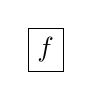
\begin{tikzpicture}
    \node at(0,0)[anchor=north, draw, rectangle]{$f$};
\end{tikzpicture}
}}
\end{equation*}
ベクトルは脚つきで表現される.
\begin{equation*}
    \text{vector}\:\bm{v}=\vcenter{\hbox{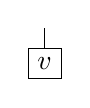
\begin{tikzpicture}
    \node at(0,0)[anchor=north, draw, rectangle](v){$\bm{v}$};
    \draw(v.north)--++(0,.25);
\end{tikzpicture}
}}
\end{equation*}
この脚は\ref{sec: Kronecker for tensor}に示すようにKroneckerの$\delta$を表す.


\subsubsection{スカラー倍}

文字式と同様, スカラーとベクトルを並べてスカラー倍を表せる.
\begin{equation*}
    fg\bm{v}
    =
    \vcenter{\hbox{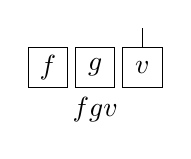
\begin{tikzpicture}
    \draw(-.6,0)rectangle(-.1,.5);
    \draw(0,0)rectangle(.5,.5);
    \draw(.6,0)rectangle(1.1,.5);
    \draw(.85,.5)--(.85,.75);
    \node[anchor=center]at(-.35,.25){$f$};
    \node[anchor=center]at(.25,.25){$g$};
    \node[anchor=center]at(.85,.25){$\bm{v}$};
    \node[anchor=north]at(.25,0){$fg\bm{v}$};
\end{tikzpicture}
}}
\end{equation*}


\subsubsection{ベクトルの内積}

ベクトルの脚を繋ぎ合わせると内積を表す.
\begin{equation*}
    \bm{u\cdot v}=u_i\delta_{ij}v_j
    =
    \vcenter{\hbox{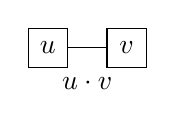
\begin{tikzpicture}
    \draw(0,0)rectangle(.5,.5);
    \draw(1.,0)rectangle(1.5,.5);
    \draw(.5,.25)--(1.,.25);
    \node[anchor=center]at(.25,.25){$\bm{u}$};
    \node[anchor=center]at(1.25,.25){$\bm{v}$};
    \node[anchor=north]at(.75,0){$\bm{u\cdot v}$};
\end{tikzpicture}
}}
\end{equation*}


\subsubsection{3成分のLevi-Civita記号}
\label{sec: vector: 3 components levicivita}

以上ではスカラーやベクトルは四角で囲って表してきたが, ベクトルの添字については四角で囲わずに表すこととする.
この約束のもと, 3成分のLevi-Civita記号は次のように表す.
\begin{equation*}
    \epsilon_{ijk}
    =
    \vcenter{\hbox{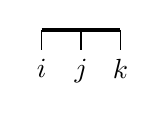
\begin{tikzpicture}
    \draw[ultra thick]
        (0,1)--(1,1)
    ;
    \draw
        (0,1)--(0,.75) node[anchor=north]{$i$}
        (.5,1)--(.5,.75) node[anchor=north]{$j$}
        (1,1)--(1,.75) node[anchor=north]{$k$}
    ;
\end{tikzpicture}
}}
\end{equation*}
太線は反対称性を表し, 脚の奇置換で符号が変わる.
\begin{equation*}
    \vcenter{\hbox{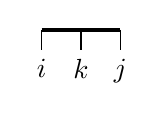
\begin{tikzpicture}
    \draw[ultra thick]
        (0,1)--(1,1)
    ;
    \draw
        (0,1)--(0,.75) node[anchor=north]{$i$}
        (.5,1)--(.5,.75) node[anchor=north]{$k$}
        (1,1)--(1,.75) node[anchor=north]{$j$}
    ;
\end{tikzpicture}
}}
    =
    -\vcenter{\hbox{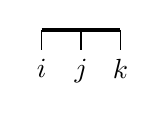
\begin{tikzpicture}
    \draw[ultra thick]
        (0,1)--(1,1)
    ;
    \draw
        (0,1)--(0,.75) node[anchor=north]{$i$}
        (.5,1)--(.5,.75) node[anchor=north]{$j$}
        (1,1)--(1,.75) node[anchor=north]{$k$}
    ;
\end{tikzpicture}
}}
\end{equation*}


\subsubsection{ベクトルの外積}

ベクトルの外積は次のように表せる.
\begin{equation*}
    \bm{u}\times\bm{v}
    =
    \vcenter{\hbox{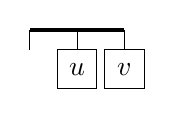
\begin{tikzpicture}
    \draw[ultra thick]
        (.25,1)--(1.45,1)
    ;
    \draw
    (.25,1)--(.25,.75)
    % node[anchor=north]{$i$}
    (.85,1)--(.85,.75)
    (1.45,1)--(1.45,.75)
    (.6,.25)rectangle(1.1,.75)
    node[anchor=center]at(.85,.5){$\bm{u}$}
    (1.2,.25)rectangle(1.7,.75)
    node[anchor=center]at(1.45,.5){$\bm{v}$}
    ;
\end{tikzpicture}
}}
\end{equation*}
一番左に脚が1本残っていることからベクトルであることが一瞥できる.



\subsection{ベクトルの内積と外積にまつわる公式}

\subsubsection{Levi-Civita記号の縮約公式}
\label{sec: levi-civita contraction for vectors}

\begin{equation*}
    \epsilon_{ijm}\epsilon_{klm}
    =
    \delta_{ik}\delta_{jl}
    -
    \delta_{il}\delta_{jk}
\end{equation*}
Levi-Civita記号の縮約公式は\ref{sec: levicivita: contraction}で詳細を取り扱うが, ここでは公式的に用いることにする.
\begin{equation*}
    \vcenter{\hbox{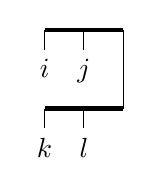
\begin{tikzpicture}
    \draw[ultra thick]
        (0,1)--(1,1)
        (0,2)--(1,2)
    ;
    \draw
        (0,1)--(0,.75) node[anchor=north]{$k$}
        (.5,1)--(.5,.75) node[anchor=north]{$l$}
        (1,1)--(1,2)
        (0,2)--(0,1.75) node[anchor=north]{$i$}
        (.5,2)--(.5,1.75) node[anchor=north]{$j$}
    ;
\end{tikzpicture}
}}
    =
    \vcenter{\hbox{\begin{tikzpicture}
    \draw
        node (i1) at (2,1.25) [anchor=south]{$i$}
        node (j1) at (2.5,1.25)[anchor=south]{$j$}
        node (k1) at (2,.75) [anchor=north]{$k$}
        node (l1) at (2.5,.75) [anchor=north]{$l$}
        (i1) -- (k1)
        (j1) -- (l1)
    ;
\end{tikzpicture}
}}
    -
    \vcenter{\hbox{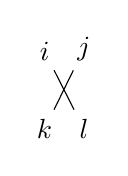
\begin{tikzpicture}
    \draw
        node (i2) at (3.5,1.25) [anchor=south]{$i$}
        node (j2) at (4,1.25)[anchor=south]{$j$}
        node (k2) at (3.5,.75) [anchor=north]{$k$}
        node (l2) at (4,.75) [anchor=north]{$l$}
        (i2)--(l2)
        (j2)--(k2)
    ;
\end{tikzpicture}
}}
\end{equation*}


\subsubsection{スカラー三重積}

\begin{equation*}
    \bm{A}\cdot(\bm{B}\times\bm{C})
    =
    \bm{B}\cdot(\bm{C}\times\bm{A})
    =
    \bm{C}\cdot(\bm{A}\times\bm{B})
    =
    -
    \bm{B}\cdot(\bm{A}\times\bm{C})
\end{equation*}
外積の脚にベクトルの脚をつなげればスカラー三重積を表せる.
\begin{equation*}
    \vcenter{\hbox{\begin{tikzpicture}
    \coordinate(origin)at(0,1);
    \draw[ultra thick]
        (origin) -- ++(1.2,0)
    ;
    \draw
        (origin) -- ++(0,-.25)
        ($(origin)+(.6,0)$) -- ++(0,-.25)
        ++(.6,0) -- ++(0,.25)
        ($(origin)+(-.25,-.75)$) rectangle ++(.5,.5)
        ++(.1,-.5) rectangle ++(.5,.5)
        ++(.1,-.5) rectangle ++(.5,.5)
        node[anchor=center]at ($(origin)+(0,-.5)$) {$\bm{A}$}
        node[anchor=center]at ($(origin)+(.6,-.5)$) {$\bm{B}$}
        node[anchor=center]at ($(origin)+(1.2,-.5)$) {$\bm{C}$}
    ;
\end{tikzpicture}
}}
    =
    \vcenter{\hbox{\begin{tikzpicture}
    \coordinate(origin)at(0,1);
    \draw[ultra thick]
        (origin) -- ++(1.2,0)
    ;
    \draw
        (origin) -- ++(0,-.25)
        ($(origin)+(.6,0)$) -- ++(0,-.25)
        ++(.6,0) -- ++(0,.25)
        ($(origin)+(-.25,-.75)$) rectangle ++(.5,.5)
        ++(.1,-.5) rectangle ++(.5,.5)
        ++(.1,-.5) rectangle ++(.5,.5)
        node[anchor=center]at ($(origin)+(0,-.5)$) {$\bm{B}$}
        node[anchor=center]at ($(origin)+(.6,-.5)$) {$\bm{C}$}
        node[anchor=center]at ($(origin)+(1.2,-.5)$) {$\bm{A}$}
    ;
\end{tikzpicture}
}}
    =
    \vcenter{\hbox{\begin{tikzpicture}
    \coordinate(origin)at(0,1);
    \draw[ultra thick]
        (origin) -- ++(1.2,0)
    ;
    \draw
        (origin) -- ++(0,-.25)
        ($(origin)+(.6,0)$) -- ++(0,-.25)
        ++(.6,0) -- ++(0,.25)
        ($(origin)+(-.25,-.75)$) rectangle ++(.5,.5)
        ++(.1,-.5) rectangle ++(.5,.5)
        ++(.1,-.5) rectangle ++(.5,.5)
        node[anchor=center]at ($(origin)+(0,-.5)$) {$\bm{C}$}
        node[anchor=center]at ($(origin)+(.6,-.5)$) {$\bm{A}$}
        node[anchor=center]at ($(origin)+(1.2,-.5)$) {$\bm{B}$}
    ;
\end{tikzpicture}
}}
    =
    -
    \vcenter{\hbox{\begin{tikzpicture}
    \coordinate(origin)at(0,1);
    \draw[ultra thick]
        (origin) -- ++(1.2,0)
    ;
    \draw
        (origin) -- ++(0,-.25)
        ($(origin)+(.6,0)$) -- ++(0,-.25)
        ++(.6,0) -- ++(0,.25)
        ($(origin)+(-.25,-.75)$) rectangle ++(.5,.5)
        ++(.1,-.5) rectangle ++(.5,.5)
        ++(.1,-.5) rectangle ++(.5,.5)
        node[anchor=center]at ($(origin)+(0,-.5)$) {$\bm{B}$}
        node[anchor=center]at ($(origin)+(.6,-.5)$) {$\bm{A}$}
        node[anchor=center]at ($(origin)+(1.2,-.5)$) {$\bm{C}$}
    ;
\end{tikzpicture}
}}
\end{equation*}
偶置換で値が変わらず奇置換で符号が変わることが一目瞭然である.


\subsubsection{ベクトル三重積}

\begin{equation*}
    \bm{A}\times(\bm{B}\times\bm{C})
    =
    \bm{B}(\bm{A\cdot C})
    -
    \bm{C}(\bm{A\cdot B})
\end{equation*}
外積の脚を外積に繋げばベクトル三重積となる.
Levi-Civita記号の縮約公式に合わせて, はじめに偶置換しておくと見やすい.
\begin{equation*}
    \vcenter{\hbox{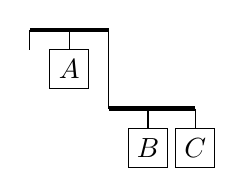
\begin{tikzpicture}
    \draw[ultra thick]
        (-4,2)--(-3,2)
        (-3,1)--(-1.9,1)
    ;
    \draw
        (-4,2)--(-4,1.75)
        (-3.5,2)--(-3.5,1.75)
        (-3.75,1.25) rectangle (-3.25,1.75)
        node[anchor=center]at(-3.5,1.5){$\bm{A}$}
        (-3,1)--(-3,2)
        (-2.5,1)--(-2.5,.75)
        (-2.25,.25)rectangle(-2.75,.75)
        node[anchor=center]at(-2.5,.5){$\bm{B}$}
        (-1.9,1)--(-1.9,.75)
        (-2.15,.25)rectangle(-1.65,.75)
        node[anchor=center]at(-1.9,.5){$\bm{C}$}
    ;
\end{tikzpicture}
}}
    =
    \vcenter{\hbox{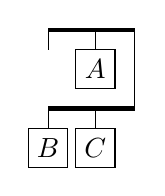
\begin{tikzpicture}
    \draw[ultra thick]
        (-.1,2)--(1,2)
        (-.1,1)--(1,1)
    ;
    \draw
        (1,1)--(1,2)
        (-.1,2)--(-.1,1.75)
        (.5,2)--(.5,1.75)
        (.25,1.25)rectangle(.75,1.75)
        node[anchor=center]at(.5,1.5){$\bm{A}$}
        (-.1,1)--(-.1,.75)
        (-.35,.25)rectangle(.15,.75)
        node[anchor=center]at(-.1,.5){$\bm{B}$}
        (.5,1)--(.5,.75)
        (.25,.25)rectangle(.75,.75)
        node[anchor=center]at(.5,.5){$\bm{C}$}
    ;
\end{tikzpicture}
}}
    =
    \vcenter{\hbox{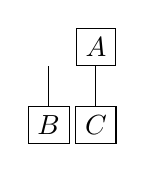
\begin{tikzpicture}
    \draw
        node[anchor=south, draw, rectangle](A1)at(3.65,1.25){$\bm{A}$}
        node[anchor=north, draw, rectangle](B1)at(3.05,.75){$\bm{B}$}
        node[anchor=north, draw, rectangle](C1)at(3.65,.75){$\bm{C}$}
        (A1.south)--(C1.north)
        (B1.north)-- ++(0,.5)
    ;
\end{tikzpicture}
}}
    -
    \vcenter{\hbox{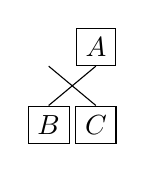
\begin{tikzpicture}
    \draw
        node[anchor=south, draw, rectangle](A2)at(5.4,1.25){$\bm{A}$}
        node[anchor=north, draw, rectangle](B2)at(4.8,.75){$\bm{B}$}
        node[anchor=north, draw, rectangle](C2)at(5.4,.75){$\bm{C}$}
        (A2.south)--(B2.north)
        (C2.north)--++(-.6,.5)
    ;
\end{tikzpicture}
}}
\end{equation*}


\subsubsection{ベクトル四重積}

\begin{equation*}
    (\bm{A}\times\bm{B})\cdot(\bm{C}\times\bm{D})
    =
    \det\mqty(
        \bm{A}\cdot\bm{C}
        &
        \bm{B}\cdot\bm{C}
        \\
        \bm{A}\cdot\bm{D}
        &
        \bm{B}\cdot\bm{D}
    )
\end{equation*}
行列式を使って表すことが多い.
行列式による表式が見やすいわけではないが, Levi-Civita記号の縮約公式が
\begin{align*}
    \epsilon_{ijm}\epsilon_{klm}
    =
    \det\mqty(
        \delta_{ik} & \delta_{il}
        \\
        \delta_{jk} & \delta_{jl}
    )
\end{align*}
と表されることを考慮すると自明であろう.
\begin{equation*}
    \vcenter{\hbox{\begin{tikzpicture}
    \coordinate(origin)at(0,2);
    \draw[ultra thick]
        (origin)--++(1.1,0)
        ($(origin)-(0,1)$)--++(1.1,0)
    ;
    \draw
        (origin)--++(0,-1)
        ++(.5,0)--++(0,-.25)
        node[anchor=north,draw,rectangle](C1){$\bm{C}$}
        ++(.6,.25)--++(0,-.25)
        node[anchor=north,draw,rectangle](D1){$\bm{D}$}
        ++(0,1.25)--++(0,-.25)
        node[anchor=north,draw,rectangle](B1){$\bm{B}$}
        ++(-.6,.25)--++(0,-.25)
        node[anchor=north,draw,rectangle](A1){$\bm{A}$}
    ;
\end{tikzpicture}
}}
    =
    \vcenter{\hbox{\begin{tikzpicture}
    \coordinate(origin)at(3,2);
    \draw
        ($(origin)+(0,-.25)$)
        node[anchor=north,draw,rectangle](A2){$\bm{A}$}
        ++(.6,0)
        node[anchor=north,draw,rectangle](B2){$\bm{B}$}
        ++(-.6,-1)
        node[anchor=north,draw,rectangle](C2){$\bm{C}$}
        ++(.6,0)
        node[anchor=north,draw,rectangle](D2){$\bm{D}$}
        (A2.south)--(C2.north)
        (B2.south)--(D2.north)
    ;
\end{tikzpicture}
}}
    -
    \vcenter{\hbox{\begin{tikzpicture}
    \coordinate(origin)at(5,2);
    \draw
        ($(origin)+(0,-.25)$)
        node[anchor=north,draw,rectangle](A2){$\bm{A}$}
        ++(.6,0)
        node[anchor=north,draw,rectangle](B2){$\bm{B}$}
        ++(-.6,-1)
        node[anchor=north,draw,rectangle](C2){$\bm{C}$}
        ++(.6,0)
        node[anchor=north,draw,rectangle](D2){$\bm{D}$}
        (A2.south)--(D2.north)
        (B2.south)--(C2.north)
    ;
\end{tikzpicture}
}}
\end{equation*}



\subsection{スカラー・ベクトルの微分作用素}

Penroseのグラフ記法で扱う微分演算子は$\nabla$(ナブラ)である.
微分対象を円で囲い, 円から脚を伸ばすことで表現する.
これもまた図形的に表すことが可能である.
\begin{equation*}
    \nabla
    =
    \vcenter{\hbox{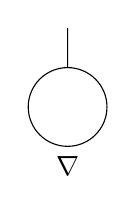
\begin{tikzpicture}
    \draw
    circle[radius=0.5]
    ++(0,.5)--++(0,.5)
    ++(0,-1.5)node[anchor=north]{$\nabla$}
    ;
\end{tikzpicture}
}}
\end{equation*}


\subsubsection{勾配 $\gradop$}

スカラーを円で囲って脚を伸ばす.
\begin{equation*}
    \gradop{f}=\nabla f
    =
    \vcenter{\hbox{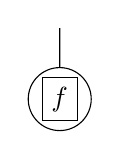
\begin{tikzpicture}
    \draw
    node[anchor=center,draw,rectangle]{$f$}
    circle[radius=0.4]
    ++(0,.4)--++(0,.5)
    ;
\end{tikzpicture}
}}
\end{equation*}


\subsubsection{発散 $\diver$}

ベクトルの脚と微分演算子の脚をつなげる.
\begin{equation*}
    \diver\bm{v}=\nabla\cdot\bm{v}
    =
    \vcenter{\hbox{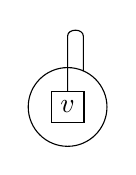
\begin{tikzpicture}
    \draw
    node[anchor=center,draw,rectangle](v){$\bm{v}$}
    (v.north)--++(0,.7)
    .. controls ++(0,.1) and ++(0,.1) .. ++(.2,0)
    --++(0,-.45)
    (v.center)circle[radius=.5]
    ;
\end{tikzpicture}
}}
\end{equation*}
脚はKroneckerの$\delta$を表すので$\partial_i\delta_{ij}v_j$を意味する.


\subsubsection{回転 $\rotop$}
\label{sec: rot}

単純な外積と表示は大きく変わらない.
ただし微分対象は演算子のすぐ右の脚に配置する.
\footnote{この追加ルールについては\ref{sec: div uv}を参照. }
\begin{equation*}
    \rotop\bm{v}=\nabla\times\bm{v}
    =
    \vcenter{\hbox{\begin{tikzpicture}
    \coordinate(origin)at(0,0);
    \draw
    (origin)--++(1,0)
    ++(0,-.05)--++(-1,0)
    (origin)--++(0,-.25)
    ++(.5,.25)--++(0,-.25)
    ($(origin)+(1,0)$)--++(0,-.25)
    node[anchor=north, draw, rectangle](v){$\bm{v}$}
    (v.center)circle[radius=.3]
    ($(origin)+(.5,-.25)$)--++(.2,-.2)
    ;
\end{tikzpicture}
}}
\end{equation*}


\subsubsection{ラプラシアン $\lapl$}
\label{sec: lapl}

2つの微分演算子の脚をつなぎ合わせる.
微分対象はスカラー・ベクトルを問わない.
\begin{equation*}
    \lapl f=\laplacian f
    =
    \vcenter{\hbox{\begin{tikzpicture}
    \coordinate(origin1)at(0,0);
    \draw
        (origin1) node[anchor=center, draw, rectangle](f){$f$}
        ($(f.north)+(0,.1)$)--++(0,.7)
        .. controls ++(0,.1) and ++(0,.1) .. ++(.2,0)
        --++(0,-.5)
        (f.center) circle[radius=.4]
        (f.center) circle[radius=.6]
    ;
\end{tikzpicture}
}},
    \qquad
    \lapl \bm{v}
    =
    \laplacian\bm{v}
    =
    \vcenter{\hbox{\begin{tikzpicture}
    \coordinate(origin2)at(2,0);
    \draw
        (origin2) node[anchor=center, draw, rectangle](v){$\bm{v}$}
        (v.north)--++(0,.5)
        ($(v.north)+(.2,.15)$)--++(0,.7)
        .. controls ++(0,.1) and ++(0,.1) .. ++(.2,0)
        --++(0,-.6)
        (v.center) circle[radius=.4]
        (v.center) circle[radius=.6]
    ;
\end{tikzpicture}
}}
\end{equation*}
$\partial_i\delta_{ij}\partial_jA$を表す.
特に微分対象がスカラーの場合, 直ちに$\diver\gradop f=\lapl f$が得られる.


\subsubsection{積の微分(Leibnitz rule)}

\begin{equation*}
    \nabla(AB)=\nabla(A)B+A\nabla(B)
\end{equation*}
微分作用素はLeibnitz ruleに従って展開可能である.
\begin{equation*}
    \vcenter{\hbox{\begin{tikzpicture}
    \coordinate(O1)at(0,0);
    \coordinate(O2)at(2.8,0);
    \coordinate(O3)at(5.6,0);
    \node[anchor=center]at(1.4,0){$=$};
    \node[anchor=center]at(4.2,0){$+$};
    \draw
    ($(O1)+(-.4,0)$) node[anchor=center,draw,rectangle]{$A$}
    ($(O1)+(.4,0)$) node[anchor=center,draw,rectangle]{$B$}
    (O1)circle[x radius=1,y radius=.4]
    ++(0,.4)--++(0,.5)
    ;
    \draw
    ($(O2)+(-.4,0)$) node[anchor=center,draw,rectangle](A){$A$}
    ($(O2)+(.4,0)$) node[anchor=center,draw,rectangle]{$B$}
    (A)circle[radius=.4]
    ++(0,.4)--++(0,.5)
    ;
    \draw
    ($(O3)+(-.4,0)$) node[anchor=center,draw,rectangle]{$A$}
    ($(O3)+(.4,0)$) node[anchor=center,draw,rectangle](B){$B$}
    (B)circle[radius=.4]
    ++(0,.4)--++(0,.5)
    ;
\end{tikzpicture}
}}
\end{equation*}


\subsubsection{微分順序交換}

$C^2$級関数(2階導関数が連続な関数)では微分順序の交換が可能である.
グラフ記法では円の内外を入れ替えることにほかならない.
\begin{equation*}
    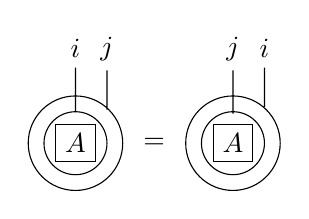
\begin{tikzpicture}
    \coordinate(origin1)at(0,0);
    \coordinate(origin2)at(2,0);
    \node at(0,1.2)[anchor=center](i1){$i$};
    \node at(.4,1.2)[anchor=center](j1){$j$};
    \node at(2.4,1.2)[anchor=center](i2){$i$};
    \node at(2.,1.2)[anchor=center](j2){$j$};
    \draw
    (origin1) node[anchor=center, draw, rectangle](A1){$A$}
    (i1.south)--++(0,-.55)
    (j1.south)--++(0,-.5)
    (A1.center) circle[radius=.4]
    (A1.center) circle[radius=.6]
    ;
    \draw
    (origin2) node[anchor=center, draw, rectangle](A2){$A$}
    (i2.south)--++(0,-.5)
    (j2.south)--++(0,-.55)
    (A2.center) circle[radius=.4]
    (A2.center) circle[radius=.6]
    ;
    \node[anchor=center]at(1,0){$=$};
\end{tikzpicture}

\end{equation*}
以降, 特に断りのない限り全ての量は$C^2$級であるとする.



\subsection{ベクトルの微分作用素にまつわる公式}

本節の公式は以下に示す5つの変形\textbf{のみ}を用いて導出が可能である.
\begin{itemize}
    \item Levi-Civita記号の反対称性(奇置換)
    \item Levi-Civita記号での偶置換
    \item Levi-Civita記号の縮約公式
    \item Leibnitz rule
    \item 微分順序交換
\end{itemize}
全ての導出はEinsteinの縮約記法を用いた方法と全く同じ手順である.


\subsubsection{$\rotop\gradop=0$}
\label{sec: rot grad}

\begin{equation*}
    \rotop\gradop f=\nabla\times\nabla f=0
\end{equation*}
微分順序の交換と反対称性を用いる.
\begin{equation*}
    \begin{tikzpicture}
    \coordinate(origin1)at(0,0);
    \coordinate(origin2)at(3,0);
    \coordinate(origin3)at(6,0);
    \node at(1,-.5)[anchor=north, draw, rectangle](v1){$f$};
    \node at(4,-.5)[anchor=north, draw, rectangle](v2){$f$};
    \node at(7,-.5)[anchor=north, draw, rectangle](v3){$f$};
    \draw[ultra thick]
        (origin1)--++(1,0)
        (origin2)--++(1,0)
        (origin3)--++(1,0)
    ;
    \draw
        (origin1)--++(0,-.25)
        ++(.5,.25)--++(0,-.25)
        ($(origin1)+(1,0)$)--++(0,-.4)
        (v1.center)circle[radius=.5]
        (v1.center)circle[radius=.4]
        ($(origin1)+(.5,-.25)$)--++(.15,-.15)
    ;
    \node at(2.25,-.5)[anchor=center]{$=$};
    \draw
        (origin2)--++(0,-.25)
        ++(.5,.25)--++(0,-.25)
        ($(origin2)+(1,0)$)--++(0,-.3)
        (v2.center)circle[radius=.5]
        (v2.center)circle[radius=.4]
        ($(origin2)+(.5,-.25)$)--++(.25,-.25)
    ;
    \node at(5.25,-.5)[anchor=center]{$=-$};
    \draw
        (origin3)--++(0,-.25)
        ++(.5,.25)--++(0,-.25)
        ($(origin3)+(1,0)$)--++(0,-.4)
        (v3.center)circle[radius=.5]
        (v3.center)circle[radius=.4]
        ($(origin3)+(.5,-.25)$)--++(.15,-.15)
    ;
\end{tikzpicture}

\end{equation*}
第1に微分順序交換, 第2に反対称.
左辺と右辺で$A=-A$の形になっているので値は$0$である.


\subsubsection{$\diver\rotop=0$}

\begin{equation*}
    \diver\rotop\bm{v}=\nabla\cdot(\nabla\times\bm{v})=0
\end{equation*}
\ref{sec: rot grad}と同様に示せる.
\begin{equation*}
    \begin{tikzpicture}
    \coordinate(origin1)at(0,0);
    \coordinate(origin2)at(3,0);
    \coordinate(origin3)at(6,0);
    \draw[ultra thick]
        (origin1)--++(1,0)
        (origin2)--++(1,0)
        (origin3)--++(1,0)
    ;
    \draw
        (origin1)--++(0,-.25)
        ++(.5,.25)--++(0,-.25)
        ($(origin1)+(1,0)$)--++(0,-.25)
        node[anchor=north, draw, rectangle](v1){$\bm{v}$}
        (v1.center)circle[radius=.3]
        (v1.center)circle[radius=.4]
        ($(origin1)+(0,-.25)$)--++(.6,-.3)
        ($(origin1)+(.5,-.25)$)--++(.2,-.2)
    ;
    \node at(2.25,-.5)[anchor=center]{$=$};
    \draw
        (origin2)--++(0,-.25)
        ++(.5,.25)--++(0,-.25)
        ($(origin2)+(1,0)$)--++(0,-.25)
        node[anchor=north, draw, rectangle](v2){$\bm{v}$}
        (v2.center)circle[radius=.3]
        (v2.center)circle[radius=.4]
        ($(origin2)+(0,-.25)$)--++(.7,-.3)
        ($(origin2)+(.5,-.25)$)--++(.1,-.1)
    ;
    \node at(5.25,-.5)[anchor=center]{$=-$};
    \draw
        (origin3)--++(0,-.25)
        ++(.5,.25)--++(0,-.25)
        ($(origin3)+(1,0)$)--++(0,-.25)
        node[anchor=north, draw, rectangle](v3){$\bm{v}$}
        (v3.center)circle[radius=.3]
        (v3.center)circle[radius=.4]
        ($(origin3)+(0,-.25)$)--++(.6,-.3)
        ($(origin3)+(.5,-.25)$)--++(.2,-.2)
    ;
\end{tikzpicture}

\end{equation*}
第1に微分順序交換, 第2に反対称.
やはり左辺と右辺で$A=-A$の形になっているので値は$0$となる.


\subsubsection{$\diver\gradop=\lapl$}

\begin{equation*}
    \diver\gradop f=\nabla\cdot\nabla f=\lapl f
\end{equation*}
\ref{sec: lapl}で紹介したが, 公式として再掲する.
\begin{equation*}
    \lapl f=\laplacian f
    =
    \vcenter{\hbox{\begin{tikzpicture}
    \coordinate(origin1)at(0,0);
    \draw
        (origin1) node[anchor=center, draw, rectangle](f){$f$}
        ($(f.north)+(0,.1)$)--++(0,.7)
        .. controls ++(0,.1) and ++(0,.1) .. ++(.2,0)
        --++(0,-.5)
        (f.center) circle[radius=.4]
        (f.center) circle[radius=.6]
    ;
\end{tikzpicture}
}}
\end{equation*}


\subsubsection{$\gradop(fg)=g\gradop f+f\gradop g$}

\begin{align*}
    &\gradop(fg)=(\gradop f)g+f(\gradop g)
    \\
    &\nabla(fg)=(\nabla f)g+f(\nabla g)
\end{align*}
Leibnitz ruleで展開する.
\begin{equation*}
    \begin{tikzpicture}
    \coordinate(origin1)at(0,0);
    \coordinate(origin2)at(2.8,0);
    \coordinate(origin3)at(5.6,0);
    \node[anchor=center]at(1.4,0){$=$};
    \node[anchor=center]at(4.2,0){$+$};
    \draw
    ($(origin1)+(-.4,0)$) node[anchor=center,draw,rectangle]{$f$}
    ($(origin1)+(.4,0)$) node[anchor=center,draw,rectangle]{$g$}
    (origin1)circle[x radius=1,y radius=.4]
    ++(0,.4)--++(0,.5)
    ;
    \draw
    ($(origin2)+(-.4,0)$) node[anchor=center,draw,rectangle](A){$f$}
    ($(origin2)+(.4,0)$) node[anchor=center,draw,rectangle]{$g$}
    (A)circle[radius=.4]
    ++(0,.4)--++(0,.5)
    ;
    \draw
    ($(origin3)+(-.4,0)$) node[anchor=center,draw,rectangle]{$f$}
    ($(origin3)+(.4,0)$) node[anchor=center,draw,rectangle](B){$g$}
    (B)circle[radius=.4]
    ++(0,.4)--++(0,.5)
    ;
\end{tikzpicture}

\end{equation*}
物理学においては, 数式でも然りだが, 誤解を生む形でなければベクトルのスカラー倍を表すのに必ずしもスカラー・ベクトルの順で配する必要はない.
グラフ記法でも同様である.


\subsubsection{$\diver(fv)=\gradop f\cdot v+f\diver v$}

\begin{align*}
    &\diver(f\bm{v})=\gradop f\cdot\bm{v}+f\diver\bm{v}
    \\
    &\nabla(f\bm{v})=\nabla f\cdot\bm{v}+f\nabla\cdot\bm{v}
\end{align*}
これもまたLeibnitz ruleで展開する.
\begin{equation*}
    \begin{tikzpicture}
    \coordinate(origin1)at(0,0);
    \coordinate(origin2)at(2.8,0);
    \coordinate(origin3)at(5.6,0);
    \node[anchor=center]at(1.4,0){$=$};
    \node[anchor=center]at(4.2,0){$+$};
    \draw
    ($(origin1)+(-.4,0)$) node[anchor=center,draw,rectangle]{$f$}
    ($(origin1)+(.4,0)$) node[anchor=center,draw,rectangle](v1){$\bm{v}$}
    (v1.north)--++(0,.7)
    (origin1)circle[x radius=1,y radius=.4]
    ++(0,.4)--++(0,.5)
    .. controls ++(0,.2) and ++(0,.2) .. ++(.4,0)
    ;
    \draw
    ($(origin2)+(-.4,0)$) node[anchor=center,draw,rectangle](f2){$f$}
    ($(origin2)+(.4,0)$) node[anchor=center,draw,rectangle](v2){$\bm{v}$}
    (f2)circle[radius=.4]
    (v2.west)--++(-.155,0)
    ;
    \draw
    ($(origin3)+(-.4,0)$) node[anchor=center,draw,rectangle]{$f$}
    ($(origin3)+(.4,0)$) node[anchor=center,draw,rectangle](v3){$\bm{v}$}
    (v3)circle[radius=.4]
    ++(.2,.35)--++(0,.5)
    (v3.north)--++(0,.65)
    .. controls ++(0,.1) and ++(0,.1) .. ++(.2,0)
    ;
\end{tikzpicture}

\end{equation*}


\subsubsection{$\diver(u\times v)=\rotop u\cdot v-u\cdot\rotop v$}
\label{sec: div uv}

\begin{align*}
    &\diver(\bm{u}\times\bm{v})=\rotop\bm{u}\cdot\bm{v}-\bm{u}\cdot\rotop\bm{v}
    \\
    &\nabla\cdot(\bm{u}\times\bm{v})=(\nabla\times\bm{u})\bm{v}-\bm{u}\cdot(\nabla\times\bm{v})
\end{align*}
Leibnitz ruleに加えて反対称性を用いる.
\begin{equation*}
    \begin{tikzpicture}
    \coordinate(origin1)at(0,0);
    \coordinate(origin2)at(3,0);
    \coordinate(origin3)at(6,0);
    \coordinate(origin4)at(3,-1.5);
    \coordinate(origin5)at(6,-1.5);
    \draw
    (origin1)--++(1,0)
    ++(0,-.05)--++(-1,0)
    (origin1)--++(0,-.25)
    ++(.5,.25)--++(0,-.25)
    node[anchor=north, draw, rectangle](u1){$\bm{u}$}
    ($(origin1)+(1,0)$)--++(0,-.25)
    node[anchor=north, draw, rectangle](v1){$\bm{v}$}
    ($(u1.center)!.5!(v1.center)$)circle[x radius=.7, y radius=.3]
    ($(origin1)+(0,-.25)$)--++(.1,-.1)
    ;
    \node at(2.125,-.5)[anchor=center]{$=$};
    \draw
    (origin2)--++(1.5,0)
    ++(0,-.05)--++(-1.5,0)
    (origin2)--++(0,-.25)
    ++(.75,.25)--++(0,-.25)
    node[anchor=north, draw, rectangle](u2){$\bm{u}$}
    ($(origin2)+(1.5,0)$)--++(0,-.25)
    node[anchor=north, draw, rectangle](v2){$\bm{v}$}
    (u2.center)circle[radius=.3]
    ($(origin2)+(0,-.25)$)--++(.45,-.3)
    ;
    \node at(5.25,-.5)[anchor=center]{$+$};
    \draw
    (origin3)--++(1.5,0)
    ++(0,-.05)--++(-1.5,0)
    (origin3)--++(0,-.25)
    ++(.75,.25)--++(0,-.25)
    node[anchor=north, draw, rectangle](u3){$\bm{u}$}
    ($(origin3)+(1.5,0)$)--++(0,-.25)
    node[anchor=north, draw, rectangle](v3){$\bm{v}$}
    (v3.center)circle[radius=.3]
    ($(origin3)+(0,-.25)$)|-++(1.4,-.5)
    ;
    \node at(2.125,-2)[anchor=center]{$=$};
    \draw
    (origin4)--++(1.5,0)
    ++(0,-.05)--++(-1.5,0)
    (origin4)--++(0,-.25)
    ++(.75,.25)--++(0,-.25)
    node[anchor=north, draw, rectangle](u4){$\bm{u}$}
    ($(origin4)+(1.5,0)$)--++(0,-.25)
    node[anchor=north, draw, rectangle](v4){$\bm{v}$}
    (u4.center)circle[radius=.3]
    ($(origin4)+(0,-.25)$)--++(.45,-.3)
    ;
    \node at(5.25,-2)[anchor=center]{$-$};
    \draw
    (origin5)--++(1.5,0)
    ++(0,-.05)--++(-1.5,0)
    (origin5)--++(0,-.25)
    node[anchor=north, draw, rectangle](u5){$\bm{u}$}
    ++(.75,.25)--++(0,-.25)
    ($(origin5)+(1.5,0)$)--++(0,-.25)
    node[anchor=north, draw, rectangle](v5){$\bm{v}$}
    (v5.center)circle[radius=.3]
    ($(origin5)+(.75,-.25)$)|-++(.45,-.2)
    ;
\end{tikzpicture}

\end{equation*}
\ref{sec: rot}で示した「rotにおいて微分対象は微分作用素のすぐ右の脚につなげる」ルールに従うようにする.


\subsubsection{$\rotop(fv)=\gradop f\times v+f\rotop v$}

\begin{align*}
    &\rotop(f\bm{v})=\gradop f\times\bm{v}+f\:\rotop\bm{v}
    \\
    &\nabla\times(f\bm{v})=\nabla f\times\bm{v}+f\nabla\times\bm{v}
\end{align*}
Leibnitz ruleによる展開.
\begin{equation*}
    \begin{tikzpicture}
    \coordinate(origin1)at(0,0);
    \coordinate(origin2)at(3,0);
    \coordinate(origin3)at(6,0);
    \draw[ultra thick]
    (origin1)--++(1.5,0)
    (origin2)--++(1.5,0)
    (origin3)--++(1.5,0)
    ;
    \draw
        (origin1)--++(0,-.25)
        ++(1.5,.25)--++(0,-.4)
        node[anchor=north, draw, rectangle](v1){$\bm{v}$}
        ++(-.5,.075) node[anchor=north, draw, rectangle](f1){$f$}
        (v1.west)circle[x radius=.7, y radius=.5]
        ($(origin1)+(.6,0)$)--++(0,-.45)
    ;
    \node at(2.5,-.5)[anchor=center]{$=$};
    \draw
        (origin2)--++(0,-.25)
        ++(1.5,.25)--++(0,-.4)
        node[anchor=north, draw, rectangle](v2){$\bm{v}$}
        ($(origin2)+(.6,0)$)--++(0,-.25)
        ++(0,-.5) node[anchor=center,draw,rectangle](f2){$f$}
        (f2.center)circle[radius=.5]
    ;
    \node at(5.25,-.5)[anchor=center]{$+$};
    \draw
        (origin3)--++(0,-.25)
        ++(1.5,.25)--++(0,-.4)
        node[anchor=north, draw, rectangle](v3){$\bm{v}$}
        ($(origin3)+(.5,0)$)--++(0,-.25)
        |-++(.5,-.2)
        ($(origin3)+(-.1,-.8)$) node[anchor=center,draw,rectangle](f3){$f$}
        (v3.center)circle[radius=.5]
    ;
\end{tikzpicture}

\end{equation*}
微分の内外を遵守する限り$f$の位置は問わない.


\subsubsection{$\rotop(u\times v)=(v\cdot\gradop)u+u\diver v-v\diver u-(u\cdot\gradop)v$}

\begin{align*}
    &\rotop(\bm{u}\times\bm{v})
    =
    (\bm{v}\cdot\gradop)\bm{u}
    +
    \bm{u}\:\diver\bm{v}
    -
    \bm{v}\:\diver\bm{u}
    -
    (\bm{u}\cdot\gradop)\bm{v}
    \\
    &\nabla\times(\bm{u}\times\bm{v})
    =
    (\bm{v}\cdot\nabla)\bm{u}
    +
    \bm{u}(\nabla\cdot\bm{v})
    -
    \bm{v}(\nabla\cdot\bm{u})
    -
    (\bm{u}\cdot\nabla)\bm{v}
\end{align*}
Levi-Civita記号の縮約公式とLeibnitz ruleによって導出.
\begin{equation*}
    \begin{tikzpicture}
    \coordinate(origin1)at(0,0);
    \node at(1.8,-1)[anchor=center]{$=$};
    \coordinate(origin2)at(2.75,-.5);
    \node at(4.1,-1)[anchor=center]{$-$};
    \coordinate(origin3)at(5,-.5);
    \node at(1.8,-2.75)[anchor=center]{$=$};
    \coordinate(origin4)at(2.75,-2);
    \node at(4.3,-2.75)[anchor=center]{$+$};
    \coordinate(origin5)at(5,-2);
    \node at(6.6,-2.75)[anchor=center]{$-$};
    \coordinate(origin6)at(7.5,-2);
    \node at(8.9,-2.75)[anchor=center]{$-$};
    \coordinate(origin7)at(9.5,-2);
    % LHS
    \draw
    (origin1)--++(1.1,0)
    ++(0,-.05)--++(-1.1,0)
    ++(0,.05)--++(0,-.25)
    ++(.6,.25)--++(0,-.25) node[anchor=north](dv1){}
    ++(.5,.25)--++(0,-1.05)
    --++(-1.1,0)
    ++(0,.05)--++(1.1,0)
    ++(-1.1,0)--++(0,-.25) node[anchor=north,draw,rectangle](u1){$\bm{u}$}
    ++(.6,.25)--++(0,-.25) node[anchor=north,draw,rectangle](v1){$\bm{v}$}
    ($(u1.center)!.5!(v1.center)$)circle[x radius=.7,y radius=.5]
    (dv1.north)--++(-.3,-.7)
    ;
    % RHS up
    \draw
    (origin2)--++(0,-.5)
    node[anchor=north,draw,rectangle](u2){$\bm{u}$}
    node at ++(.6,0)[anchor=north,draw,rectangle](v2){$\bm{v}$}
    (v2.north)--++(0,.5)
    .. controls ++(0,.2) and ++(0,.2) .. ++(-.2,0)
    -- ++(0,-.2)
    ($(u2.center)!.5!(v2.center)$) circle[x radius=.7,y radius=.5]
    ;
    \draw
    (origin3)--++(.6,-.5)
    node[anchor=north,draw,rectangle](v3){$\bm{v}$}
    node at ++(-.6,0)[anchor=north,draw,rectangle](u3){$\bm{u}$}
    (u3.north)--++(.6,.5)
    .. controls ++(.1,.1) and ++(0,.1) .. ++(.2,0)
    -- ++(0,-.35)
    ($(u3.center)!.5!(v3.center)$) circle[x radius=.7,y radius=.5]
    ;
    % RHS down
    \draw
    (origin4)--++(0,-.5)
    node[anchor=north,draw,rectangle](u4){$\bm{u}$}
    ++(.8,0) node[anchor=north,draw,rectangle](v4){$\bm{v}$}
    (u4)circle[radius=.4]
    (v4.west)--++(-.155,0)
    ;
    \draw
    (origin5)--++(0,-.5)
    node[anchor=north,draw,rectangle](u5){$\bm{u}$}
    ++(.8,0) node[anchor=north,draw,rectangle](v5){$\bm{v}$}
    (v5)circle[radius=.4]
    (v5.north)--++(0,.5)
    .. controls ++(0,.1) and ++(0,.1) .. ++(.2,0)
    --++(0,-.35)
    ;
    \draw
    (origin6)--++(0,-.5)
    node[anchor=north,draw,rectangle](u6){$\bm{u}$}
    ++(.8,0) node[anchor=north,draw,rectangle](v6){$\bm{v}$}
    (u6.center)circle[radius=.4]
    (v6.north)--++(0,.5)
    (origin6) .. controls ++(0,.1) and ++(0,.1) .. ++(.2,0)
    --++(0,-.35)
    ;
    \draw
    ($(origin7)+(0,-.5)$) node[anchor=north,draw,rectangle](u7){$\bm{u}$}
    ++(.8,0) node[anchor=north,draw,rectangle](v7){$\bm{v}$}
    (v7.north)--++(0,.5)
    (v7.center)circle[radius=.4]
    (u7.east)--++(.155,0)
    ;
\end{tikzpicture}

\end{equation*}


\subsubsection{$\rotop\rotop=\gradop\diver-\lapl$}

\begin{align*}
    &\rotop\rotop\bm{v}=\gradop\diver\bm{v}-\lapl\bm{v}
    \\
    &\nabla\times(\nabla\times\bm{v})=\nabla(\nabla\cdot\bm{v})-(\nabla\cdot\nabla)\bm{v}
\end{align*}
Levi-Civita記号の縮約公式と微分順序交換から.
\begin{equation*}
    \begin{tikzpicture}
    \coordinate(origin1)at(0,0);
    \node at(1.8,-1)[anchor=center]{$=$};
    \coordinate(origin2)at(2.75,-.5);
    \node at(3.6,-1)[anchor=center]{$-$};
    \coordinate(origin3)at(4.5,-.5);
    \node at(5.4,-1)[anchor=center]{$=$};
    \coordinate(origin4)at(6.25,-.5);
    \node at(7.1,-1)[anchor=center]{$-$};
    \coordinate(origin5)at(8,-.5);
    % LHS
    \draw[ultra thick]
        (origin1)--++(1.1,0)
        ($(origin1)-(0,1)$)--++(1.1,0)
    ;
    \draw
        (origin1)--++(0,-.25)
        ++(.6,.25)--++(0,-.25) node[anchor=north](dv1){}
        ++(.5,.25)--++(0,-1.0)
        ($(origin1)+(0.6,-1)$)--++(0,-.25) node[anchor=north,draw,rectangle](v1){$\bm{v}$}
        (v1.center)circle[radius=.3]
        (v1.center)circle[radius=.4]
        (dv1.north)--++(.2,-.85)
        ($(origin1)+(0,-1)$)|-++(.3,-.4)
    ;
    % RHS up
    \draw
        ($(origin2)+(0,-.5)$)
        node[anchor=north,draw,rectangle](v2){$\bm{v}$}
        (v2.north)--++(0,.5)
        .. controls ++(0,.1) and ++(0,.1) .. ++(-.2,0)
        -- ++(0,-.35)
        (v2.center)circle[radius=.4]
        (v2.center)circle[radius=.3]
        ($(v2.center)+(.15,.25)$)--++(0,.45)
    ;
    \draw
        ($(origin3)+(0,-.5)$)
        node[anchor=north,draw,rectangle](v3){$\bm{v}$}
        (v3.north)--++(0,.5)
        ($(v3.north)+(.1,.2)$)--++(0,.4)
        .. controls ++(0,.1) and ++(0,.1) .. ++(.2,0)
        --++(0,-.7)
        (v3.center) circle[radius=.4]
        (v3.center) circle[radius=.3]
    ;
    \draw
        ($(origin4)+(0,-.5)$)
        node[anchor=north,draw,rectangle](v4){$\bm{v}$}
        (v4.north)--++(0,.5)
        .. controls ++(0,.1) and ++(0,.1) .. ++(-.1,0)
        -- ++(0,-.425)
        (v4.center)circle[radius=.4]
        (v4.center)circle[radius=.3]
        ($(v4.center)+(.15,.375)$)--++(0,.45)
    ;
    \draw
        ($(origin5)+(0,-.5)$)
        node[anchor=north,draw,rectangle](v5){$\bm{v}$}
        (v5.north)--++(0,.5)
        ($(v5.north)+(.1,.2)$)--++(0,.4)
        .. controls ++(0,.1) and ++(0,.1) .. ++(.2,0)
        --++(0,-.7)
        (v5.center) circle[radius=.4]
        (v5.center) circle[radius=.3]
    ;
\end{tikzpicture}

\end{equation*}


\subsubsection{$\gradop(u\cdot v)=v\times\rotop u+(v\cdot\gradop)u+u\times\rotop v+(u\cdot\gradop)v$}

\begin{align*}
    &
    \gradop(\bm{u}\cdot\bm{v})
    =
    \bm{v}\times\rotop\bm{u}+(\bm{v}\cdot\gradop)\bm{u}
    +
    \bm{u}\times\rotop\bm{v}+(\bm{u}\cdot\gradop)\bm{v}
    \\
    &
    \nabla(\bm{u}\cdot\bm{v})
    =
    \bm{v}\times(\nabla\times\bm{u})+(\bm{v}\cdot\nabla)\bm{u}
    +
    \bm{u}\times(\nabla\times\bm{v})+(\bm{u}\cdot\nabla)\bm{v}
\end{align*}
初手は順当にLeibnitz ruleで展開する.
\begin{equation}
    \label{figeq: vector: grad-uv1}
    \vcenter{\hbox{\begin{tikzpicture}
    \coordinate(origin1)at(0,0);
    \coordinate(origin2)at(2.8,0);
    \coordinate(origin3)at(5.6,0);
    \node[anchor=center]at(1.4,0){$=$};
    \node[anchor=center]at(4.2,0){$+$};
    \draw
    ($(origin1)+(-.4,0)$) node[anchor=center,draw,rectangle](u1){$\bm{u}$}
    ($(origin1)+(.4,0)$) node[anchor=center,draw,rectangle](v1){$\bm{v}$}
    (origin1)circle[x radius=1,y radius=.4]
    ++(0,.4)--++(0,.5)
    (u1.east)--(v1.west)
    ;
    \draw
    ($(origin2)+(-.4,0)$) node[anchor=center,draw,rectangle](u2){$\bm{u}$}
    ($(origin2)+(.4,0)$) node[anchor=center,draw,rectangle](v2){$\bm{v}$}
    (u2)circle[radius=.4]
    ++(0,.4)--++(0,.5)
    (u2.east)--(v2.west)
    ;
    \draw
    ($(origin3)+(-.4,0)$) node[anchor=center,draw,rectangle](u3){$\bm{u}$}
    ($(origin3)+(.4,0)$) node[anchor=center,draw,rectangle](v3){$\bm{v}$}
    (v3)circle[radius=.4]
    ++(0,.4)--++(0,.5)
    (u3.east)--(v3.west)
    ;
\end{tikzpicture}
}}
\end{equation}
展開した形に相当する演算がないので, 各項Levi-Civita記号の縮約公式から得られたものとみて計算する.
右辺第1項は次のLevi-Civita記号の縮約公式から現れる.
\begin{equation*}
    \begin{tikzpicture}
    \coordinate(origin1)at(0,0);
    \node at(1.8,-1)[anchor=center]{$=$};
    \coordinate(origin2)at(3,-1);
    \node at(4.1,-1)[anchor=center]{$-$};
    \coordinate(origin3)at(5,-.25);
    % LHS
    \draw
    (origin1)--++(1.1,0)
    ++(0,-.05)--++(-1.1,0)
    ++(0,.05)--++(0,-.25)
    ++(.6,.25)--++(0,-.25) node[anchor=north,draw,rectangle](v1){$\bm{v}$}
    ++(.5,.25)--++(0,-1.05)
    --++(-1.1,0)
    ++(0,.05)--++(1.1,0)
    ++(-1.1,0)--++(0,-.25) node[anchor=north](dv1){}
    ++(.6,.25)--++(0,-.25) node[anchor=north,draw,rectangle](u1){$\bm{u}$}
    (u1.center)circle[radius=.3]
    (dv1.north)|-++(.3,-.3)
    ;
    % RHS up
    \draw
    ($(origin2)+(-.4,0)$) node[anchor=center,draw,rectangle](u2){$\bm{u}$}
    ($(origin2)+(.4,0)$) node[anchor=center,draw,rectangle](v2){$\bm{v}$}
    (u2)circle[radius=.4]
    ++(0,.4)--++(0,.5)
    (u2.east)--(v2.west)
    ;
    \draw
    (origin3)--++(0,-.5)
    node[anchor=north,draw,rectangle](u3){$\bm{u}$}
    ++(.8,0) node[anchor=north,draw,rectangle](v3){$\bm{v}$}
    (u3)circle[radius=.4]
    (v3.west)--++(-.155,0)
    ;
\end{tikzpicture}

\end{equation*}
この右辺第2項を移項したものが\eqref{figeq: vector: grad-uv1}第1項に一致する.
\eqref{figeq: vector: grad-uv1}第2項は$\bm{u},\bm{v}$を入れ替えたものに他ならない.
結局以下の図式を得る.
\begin{equation*}
    \begin{tikzpicture}
    \coordinate(origin1)at(0,0);
    \coordinate(origin2)at(2.5,1);
    \coordinate(origin3)at(5,.5);
    \coordinate(origin4)at(7.5,1);
    \coordinate(origin5)at(10,.5);
    \node[anchor=center]at(1.75,0){$=$};
    \node[anchor=center]at(4.2,0){$+$};
    \node[anchor=center]at(6.75,0){$+$};
    \node[anchor=center]at(9.2,0){$+$};

    % LHS
    \draw
        ($(origin1)+(-.4,0)$) node[anchor=center,draw,rectangle](u1){$\bm{u}$}
        ($(origin1)+(.4,0)$) node[anchor=center,draw,rectangle](v1){$\bm{v}$}
        (origin1)circle[x radius=1,y radius=.4]
        ++(0,.4)--++(0,.5)
        (u1.east)--(v1.west)
    ;
    % 1st
    \draw[ultra thick]
        (origin2)--++(1.1,0)
        ($(origin2)-(0,1)$)--++(1.1,0)
    ;
    \draw
        (origin2)--++(0,-.25)
        ++(.6,.25)--++(0,-.25) node[anchor=north,draw,rectangle](v1){$\bm{v}$}
        ++(.5,.25)--++(0,-1.0)
        ($(origin2)-(0,1)$)--++(0,-.25) node[anchor=north](dv1){}
        ++(.6,.25)--++(0,-.25) node[anchor=north,draw,rectangle](u1){$\bm{u}$}
        (u1.center)circle[radius=.3]
        (dv1.north)|-++(.3,-.3)
    ;
    % 2nd
    \draw
        (origin3)--++(0,-.5)
        node[anchor=north,draw,rectangle](u3){$\bm{u}$}
        ++(.8,0) node[anchor=north,draw,rectangle](v3){$\bm{v}$}
        (u3)circle[radius=.4]
        (v3.west)--++(-.155,0)
    ;
    % 3rd
    \draw[ultra thick]
        (origin4)--++(1.1,0)
        ($(origin4)-(0,1)$)--++(1.1,0)
    ;
    \draw
        (origin4)--++(0,-.25)
        ++(.6,.25)--++(0,-.25) node[anchor=north,draw,rectangle](v1){$\bm{u}$}
        ++(.5,.25)--++(0,-1.0)
        ($(origin4)-(0,1)$)--++(0,-.25) node[anchor=north](dv1){}
        ++(.6,.25)--++(0,-.25) node[anchor=north,draw,rectangle](u1){$\bm{v}$}
        (u1.center)circle[radius=.3]
        (dv1.north)|-++(.3,-.3)
    ;
    % 4th
    \draw
        (origin5)--++(0,-.5)
        node[anchor=north,draw,rectangle](u3){$\bm{v}$}
        ++(.8,0) node[anchor=north,draw,rectangle](v3){$\bm{u}$}
        (u3)circle[radius=.4]
        (v3.west)--++(-.155,0)
    ;
\end{tikzpicture}

\end{equation*}


\subsubsection{$\lapl(fg)=(\lapl f)g+2\:\gradop f\cdot\gradop g+f(\lapl g)$}

\begin{align*}
    &\lapl(fg)
    =
    (\lapl f)g+2\:\gradop f\cdot\gradop g+f(\lapl g)
    \\
    &\nabla\cdot\nabla(fg)
    =
    (\nabla\cdot\nabla f)g+2(\nabla f)\cdot(\nabla g)+f(\nabla\cdot\nabla g)
\end{align*}
2回にわたってLeibnitz ruleを使う.
\begin{equation*}
    \begin{tikzpicture}
    \coordinate(origin1)at(0,0);
    \coordinate(origin2)at(2.8,0);
    \coordinate(origin3)at(5.6,0);
    \coordinate(origin4)at(2.8,-2);
    \coordinate(origin5)at(5.6,-2);
    \coordinate(origin6)at(8.4,-2);
    \coordinate(origin7)at(11.2,-2);
    \node[anchor=center]at(1.4,0){$=$};
    \node[anchor=center]at(4.2,0){$+$};
    \node[anchor=center]at(1.4,-2){$=$};
    \node[anchor=center]at(4.2,-2){$+$};
    \node[anchor=center]at(7,-2){$+$};
    \node[anchor=center]at(9.8,-2){$+$};
    % LHS
    \draw
    ($(origin1)+(-.4,0)$) node[anchor=center,draw,rectangle]{$f$}
    ($(origin1)+(.4,0)$) node[anchor=center,draw,rectangle]{$g$}
    (origin1)circle[x radius=1,y radius=.4]
    (origin1)circle[x radius=1.1,y radius=.5]
    ++(0,.4)--++(0,.5)
    .. controls ++(.1,.2) .. ++(.2,0)
    --++(0,-.4)
    ;
    % RHS up
    \draw
    ($(origin2)+(-.4,0)$) node[anchor=center,draw,rectangle](A){$f$}
    ($(origin2)+(.4,0)$) node[anchor=center,draw,rectangle]{$g$}
    (A)circle[radius=.4]
    ++(0,.4)--++(0,.5)
    (origin2)circle[x radius=1.1,y radius=.5]
    ++(0,.5)--++(0,.4)
    .. controls ++(0,.1) and ++(0,.1) .. ++(-.4,0)
    ;
    \draw
    ($(origin3)+(-.4,0)$) node[anchor=center,draw,rectangle]{$f$}
    ($(origin3)+(.4,0)$) node[anchor=center,draw,rectangle](B){$g$}
    (B)circle[radius=.4]
    ++(0,.4)--++(0,.5)
    (origin3)circle[x radius=1.1,y radius=.5]
    ++(0,.5)--++(0,.4)
    .. controls ++(0,.1) and ++(0,.1) .. ++(.4,0)
    ;
    % RHS down
    \draw
    ($(origin4)+(-.4,0)$) node[anchor=center,draw,rectangle](A){$f$}
    ($(origin4)+(.4,0)$) node[anchor=center,draw,rectangle]{$g$}
    (A)circle[radius=.4]
    ++(0,.4)--++(0,.5)
    .. controls ++(0,.1) and ++(0,.1) .. ++(.2,0)
    --++(0,-.45)
    (A)circle[radius=.5]
    ;
    \draw
    ($(origin5)+(-.5,0)$) node[anchor=center,draw,rectangle](A){$f$}
    ($(origin5)+(.5,0)$) node[anchor=center,draw,rectangle](B){$g$}
    (A)circle[radius=.4]
    ++(.4,0)--++(.2,0)
    (B)circle[radius=.4]
    ;
    \draw
    ($(origin6)+(-.5,0)$) node[anchor=center,draw,rectangle](A){$f$}
    ($(origin6)+(.5,0)$) node[anchor=center,draw,rectangle](B){$g$}
    (A)circle[radius=.4]
    ++(.4,0)--++(.2,0)
    (B)circle[radius=.4]
    ;
    \draw
    ($(origin7)+(-.4,0)$) node[anchor=center,draw,rectangle]{$f$}
    ($(origin7)+(.4,0)$) node[anchor=center,draw,rectangle](B){$g$}
    (B)circle[radius=.4]
    ++(0,.4)--++(0,.5)
    .. controls ++(0,.1) and ++(0,.1) .. ++(.2,0)
    --++(0,-.45)
    (B)circle[radius=.5]
    ;
\end{tikzpicture}

\end{equation*}



\subsection{位置ベクトルの微分にまつわる公式}

位置ベクトルを$\nabla$で微分する際は次の縮約が可能である.
\begin{equation*}
    \pdv{r_i}r_j\bm{e}_j=\delta_{ij}\bm{e}_j
\end{equation*}
これをPenroseのグラフ記法で表すと, $\bm{r}$とそれを囲う円が消えて両端がつながったように表される.
\begin{equation*}
    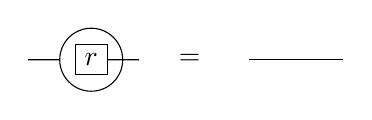
\begin{tikzpicture}
    \coordinate(origin1)at(0,0);
    \node at(1.25,0) [anchor=center]{$=$};
    \coordinate(origin2)at(2,0);
    \draw
    (origin1)node[anchor=center,draw,rectangle](r1){$\bm{r}$}
    (origin1.center)circle[radius=.4]
    ++(-.4,0)--++(-.4,0)
    (r1.east)--++(.4,0)
    ;
    \draw
    (origin2)--++(1.2,0)
    ;
\end{tikzpicture}

\end{equation*}
以下では「公式」とするにふさわしいものを拾っていくことにする.


\subsubsection{$\diver r=3$}

\begin{equation*}
    \diver\bm{r}=\nabla\cdot\bm{r}=\delta_{ii}=3
\end{equation*}
右辺の$3$は次元の数で, 4次元なら$4$, $n$次元なら$n$となる.
\begin{equation*}
    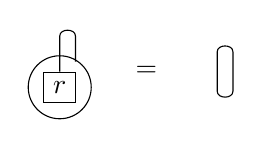
\begin{tikzpicture}
    \coordinate(origin1)at(0,0);
    \node at(1.1,0)[anchor=center]{$=$};
    \coordinate(origin2)at(2,-.25);
    \draw
    (origin1)node[anchor=north,draw,rectangle](r2){$\bm{r}$}
    (r2.center)circle[radius=.4]
    (r2.north)--++(0,.45)
    .. controls ++(0,.1) and ++(0,.1) .. ++(.2,0)
    --++(0,-.325)
    ;
    \draw
    (origin2)--++(0,.5)
    .. controls ++(0,.1) and ++(0,.1) ..++(.2,0)
    --++(0,-.5)
    .. controls ++(0,-.1) and ++(0,-.1) .. ++(-.2,0)
    ;
\end{tikzpicture}

\end{equation*}
右辺の環はKroneckerの$\delta$の両端がつながったものであり$\delta_{ii}$となる.
縮約のルールに則って3次元なら$i=1,2,3$で足し合わせる.


\subsubsection{$\rotop r=0$}

\begin{equation*}
    \rotop\bm{r}=\nabla\times\bm{r}=0
\end{equation*}
位置ベクトルの微分の縮約をとる.
\begin{equation*}
    \begin{tikzpicture}
    \coordinate(origin)at(0,0);
    \node at(2,0)[anchor=center]{$=$};
    \coordinate(origin2)at(3,0);
    \draw
    (origin)--++(1,0)
    ++(0,-.05)--++(-1,0)
    (origin)--++(0,-.25)
    ++(.5,.25)--++(0,-.25)
    ($(origin)+(1,0)$)--++(0,-.25)
    node[anchor=north, draw, rectangle](v){$\bm{r}$}
    (v.center)circle[radius=.3]
    ($(origin)+(.5,-.25)$)--++(.2,-.2)
    ;
    \draw
    (origin2)--++(1,0)
    ++(0,-.05)--++(-1,0)
    (origin)--++(0,-.25)
    ++(.5,.25)--++(0,-.25)
    ($(origin2)+(1,0)$)--++(0,-.25)
    --++(-.5,0)
    (origin2)--++(0,-.25)
    ++(.5,.25)--++(0,-.25)
    ;
\end{tikzpicture}

\end{equation*}
右辺は$\epsilon_{ijk}\delta_{jk}=\epsilon_{ijj}$を表すので$0$である.



\end{document}


\pagebreak

\documentclass[dvipdfmx]{jsarticle}
\usepackage{penrosetensor}

\begin{document}

\section{完全反対称Levi-Civita記号の公式の表現}
\label{sec: Levi-Civita}

\subsection{前提知識}

本節では,
\begin{itemize}
    \item 添字の上下
    \item 完全反対称Levi-Civita記号
    \item Einsteinの縮約記法
    \item Kroneckerの$\delta$
\end{itemize}
についての知識を前提とする.


\subsection{Penroseのグラフ記法におけるテンソルの表記}

Penroseのグラフ記法にてテンソルは階数のぶんだけ脚が出ているものとして表現される.
共変と反変の区別も可能で, 添字の上下に合わせて脚の向きが対応する.
\begin{equation*}
    T^{ij}_k
    =
    \vcenter{\hbox{\begin{tikzpicture}
    \coordinate(origin1)at(0,0);
    \coordinate(origin2)at(1,0);
    \draw
    (origin1)node[anchor=center](T1){$T$}
    ($(T1.south west)+(-.2,0)$)rectangle($(T1.north east)+(.2,0)$)
    (T1.north west)--++(0,.3)
    node[anchor=south]{$i$}
    (T1.north)--++(0,.3)
    node[anchor=south]{$j$}
    (T1.south east)--++(0,-.3)
    node[anchor=north]{$k$}
    ;
    % \node at(origin2)[anchor=west]{$T^{ij}_{\;\;\;k}$};
\end{tikzpicture}
}}
\end{equation*}
上向きの脚が反変成分, 下向きが共変を表す.


\subsubsection{Kroneckerの$\delta$}
\label{sec: Kronecker for tensor}

Kroneckerの$\delta$は両端が開いた脚で表す.
\begin{equation*}
    \delta^i_j
    =
    \vcenter{\hbox{\begin{tikzpicture}
    \draw
    node[anchor=south](i){$i$}
    (i.south)
    --++(0,-.2)
    .. controls ++(0,-.2) and ++(0,.2) .. ++(.3,-.6)
    --++(0,-.2)
    node[anchor=north]{$j$}
    ;
    % \node at(1,-.5)[anchor=west]{$\delta^i_{\;\;j}$};
\end{tikzpicture}
}}
\end{equation*}


\subsubsection{完全反対称Levi-Civitaテンソル}

横向き太線は反対称性を表し, これによって完全反対称Levi-Civitaテンソルを表現できる.
\begin{equation*}
    \epsilon_{ij\cdots k}
    =
    \vcenter{\hbox{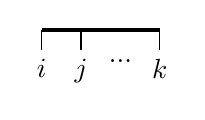
\begin{tikzpicture}
    \coordinate(origin1)at(0,.25);
    \draw[ultra thick]
        (origin1)--++(1.5,0)
    ;
    \draw
        (origin1)--++(0,-.25)
        node[anchor=north]{$i$}
        ++(.5,.25)--++(0,-.25)
        node[anchor=north]{$j$}
        ++(.5,0)node[anchor=north]{$...$}
        ++(.5,.25)--++(0,-.25)
        node[anchor=north]{$k$}
    ;
\end{tikzpicture}
}},
    \qquad
    \epsilon^{ij\cdots k}
    =
    \vcenter{\hbox{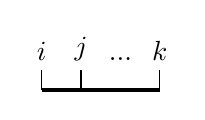
\begin{tikzpicture}
    \coordinate(origin1)at(0,.25);
    \coordinate(origin2)at(5,-.25);
    \draw[ultra thick]
        (origin2)--++(1.5,0)
    ;
    \draw
        (origin2)--++(0,.25)
        node[anchor=south]{$i$}
        ++(.5,-.25)--++(0,.25)
        node[anchor=south]{$j$}
        ++(.5,0)node[anchor=south]{$...$}
        ++(.5,-.25)--++(0,.25)
        node[anchor=south]{$k$}
    ;
\end{tikzpicture}
}}
\end{equation*}
Penroseの論文\cite{Penrose article}に合わせて階数が等しいLevi-Civitaテンソルの積は以下のように表すこともできる.
\footnote{Levi-Civitaテンソルの積というよりも「反対称化」の方が言葉は適しているだろう. $M^iB^j-B^iM^j$のような反対称テンソルを形成するときにはこの記法が有用である. }
\begin{equation*}
    \epsilon^{ij\cdots k}_{pq\cdots r}
    =
    \vcenter{\hbox{\begin{tikzpicture}
    \coordinate(origin)at(0,0);
    \draw[ultra thick]
        (origin)--++(1.5,0)
    ;
    \draw
        ($(origin)+(0,-.25)$)node[anchor=north]{$p$}
        --++(0,.5)node[anchor=south]{$i$}
        ++(.5,0)node[anchor=south]{$j$}
        --++(0,-.5)node[anchor=north]{$q$}
        ++(.5,0)node[anchor=north]{$\cdots$}
        ++(0,.5)node[anchor=south]{$\cdots$}
        ++(.5,0)node[anchor=south]{$k$}
        --++(0,-.5)
        node[anchor=north]{$r$}
        % ($(origin)+(2,0)$)node[anchor=west]{$\epsilon^{ij...k}\epsilon_{pq...r}$}
    ;
\end{tikzpicture}
}}
\end{equation*}
この正当性は
\begin{equation}
    \label{eq: Levi-Civita: product of Levi-Civita}
    \epsilon^{i_1\dots i_n}
    \epsilon_{j_1\dots j_n}
    =
    \epsilon^{i_1\dots i_n}_{1\dots n}
    \epsilon_{j_1\dots j_n}^{1\dots n}
    =
    \epsilon^{i_1\dots i_n}_{j_1\dots j_n}
\end{equation}
により保証される.


\subsubsection{計量テンソル}

計量テンソルは反変・共変に合わせてKroneckerの$\delta$を曲げたような格好になる.
\begin{equation*}
    g^{ij}
    =
    \vcenter{\hbox{\begin{tikzpicture}
    \coordinate(origin1)at(0,0);
    \coordinate(origin2)at(3,0);
    \draw
    (origin1)node[anchor=south]{$i$}
    --++(0,-.3)
    .. controls ++(0,-.3) and ++(0,-.3) .. ++(.4,0)
    --++(0,.3)
    node[anchor=south]{$j$}
    ;
\end{tikzpicture}
}},
    \qquad
    g_{ij}
    =
    \vcenter{\hbox{\begin{tikzpicture}
    \coordinate(origin1)at(0,0);
    \coordinate(origin2)at(3,0);
    \draw
    (origin2)node[anchor=north]{$i$}
    --++(0,.3)
    .. controls ++(0,.3) and ++(0,.3) .. ++(.4,0)
    --++(0,-.3)
    node[anchor=north]{$j$}
    ;
\end{tikzpicture}
}}
\end{equation*}


\subsection{Levi-Civitaテンソルの縮約公式}
\label{sec: levicivita: contraction}

\eqref{eq: Levi-Civita: product of Levi-Civita}を背景に, Euclid計量におけるLevi-Civitaテンソルの縮約はKroneckerの$\delta$の行列式を使って表されることが多い.
\begin{equation*}
    \epsilon^{ij\cdots k}\epsilon_{pq\cdots r}
    =
    \mqty|
        \delta^i_p & \delta^i_q & \cdots & \delta^i_r
        \\
        \delta^j_p & \delta^j_q & \cdots & \delta^j_r
        \\
        \vdots & \vdots & \ddots & \ddots
        \\
        \delta^k_p & \delta^k_q & \cdots & \delta^k_r
    |
\end{equation*}
一般次元, 一般計量での展開をPenroseのグラフ記法で表すと混乱を生じるので, はじめに3次元, 4次元のEuclid計量における縮約公式を取り上げる.


\subsubsection{3次元での縮約}

Kroneckerの$\delta$を使って縮約を愚直に書き出すと以下のようになる.
\begin{align*}
    \epsilon^{ijk}\epsilon_{pqr}
    &=
    \mqty|
        \delta^i_p & \delta^i_q & \delta^i_r
        \\
        \delta^j_p & \delta^j_q & \delta^j_r
        \\
        \delta^k_p & \delta^k_q & \delta^k_r
    |
    \\
    &=
    \delta^i_p\delta^j_q\delta^k_r
    -
    \delta^i_p\delta^j_r\delta^k_q
    +
    \delta^i_q\delta^j_r\delta^k_p
    -
    \delta^i_q\delta^j_p\delta^k_r
    +
    \delta^i_r\delta^j_p\delta^k_q
    -
    \delta^i_r\delta^j_q\delta^k_p
\end{align*}
\begin{equation*}
    \begin{tikzpicture}
    \coordinate(origin1)at(0,0);
    \node at(1.5,-.275)[anchor=center]{$=$};
    \coordinate(origin2)at(2,0);
    \node at(3.5,-.275)[anchor=center]{$-$};
    \coordinate(origin3)at(4,0);
    \node at(5.5,-.275)[anchor=center]{$+$};
    \coordinate(origin4)at(6,0);
    \node at(7.5,-.275)[anchor=center]{$-$};
    \coordinate(origin5)at(8,0);
    \node at(9.5,-.275)[anchor=center]{$+$};
    \coordinate(origin6)at(10,0);
    \node at(11.5,-.275)[anchor=center]{$-$};
    \coordinate(origin7)at(12,0);
    \draw[ultra thick]
        ($(origin1)+(0,-.25)$)--++(1,0)
    ;
    \draw
        (origin1)node[anchor=south]{$i$}
        --++(0,-.5)node[anchor=north]{$p$}
        ++(.5,.5)node[anchor=south]{$j$}
        --++(0,-.5)node[anchor=north]{$q$}
        ++(.5,.5)node[anchor=south]{$k$}
        --++(0,-.5)node[anchor=north]{$r$}
    ;
    \draw
        (origin2)node[anchor=south](i){$i$}
        ++(.5,0)node[anchor=south](j){$j$}
        ++(.5,0)node[anchor=south](k){$k$}
        ++(-1,-.55)node[anchor=north](p){$p$}
        ++(.5,0)node[anchor=north](q){$q$}
        ++(.5,0)node[anchor=north](r){$r$}
        (i.south)--(p.north)
        (j.south)--(q.north)
        (k.south)--(r.north)
    ;
    \draw
    (origin3)node[anchor=south](i){$i$}
    ++(.5,0)node[anchor=south](j){$j$}
    ++(.5,0)node[anchor=south](k){$k$}
    ++(-1,-.55)node[anchor=north](p){$p$}
    ++(.5,0)node[anchor=north](q){$q$}
    ++(.5,0)node[anchor=north](r){$r$}
    (i.south)--(p.north)
    (j.south)--(r.north)
    (k.south)--(q.north)
    ;
    \draw
    (origin4)node[anchor=south](i){$i$}
    ++(.5,0)node[anchor=south](j){$j$}
    ++(.5,0)node[anchor=south](k){$k$}
    ++(-1,-.55)node[anchor=north](p){$p$}
    ++(.5,0)node[anchor=north](q){$q$}
    ++(.5,0)node[anchor=north](r){$r$}
    (i.south)--(q.north)
    (j.south)--(r.north)
    (k.south)--(p.north)
    ;
    \draw
    (origin5)node[anchor=south](i){$i$}
    ++(.5,0)node[anchor=south](j){$j$}
    ++(.5,0)node[anchor=south](k){$k$}
    ++(-1,-.55)node[anchor=north](p){$p$}
    ++(.5,0)node[anchor=north](q){$q$}
    ++(.5,0)node[anchor=north](r){$r$}
    (i.south)--(q.north)
    (j.south)--(p.north)
    (k.south)--(r.north)
    ;
    \draw
    (origin6)node[anchor=south](i){$i$}
    ++(.5,0)node[anchor=south](j){$j$}
    ++(.5,0)node[anchor=south](k){$k$}
    ++(-1,-.55)node[anchor=north](p){$p$}
    ++(.5,0)node[anchor=north](q){$q$}
    ++(.5,0)node[anchor=north](r){$r$}
    (i.south)--(r.north)
    (j.south)--(p.north)
    (k.south)--(q.north)
    ;
    \draw
    (origin7)node[anchor=south](i){$i$}
    ++(.5,0)node[anchor=south](j){$j$}
    ++(.5,0)node[anchor=south](k){$k$}
    ++(-1,-.55)node[anchor=north](p){$p$}
    ++(.5,0)node[anchor=north](q){$q$}
    ++(.5,0)node[anchor=north](r){$r$}
    (i.south)--(r.north)
    (j.south)--(q.north)
    (k.south)--(p.north)
    ;
\end{tikzpicture}

\end{equation*}
上3本と下3本の端をつなぐ方法を全て列挙し, 置換に応じた符号を与えれば良い.

Levi-Civitaテンソルのグラフ記法が真価を発揮するのは一部の脚がつながっている場合だろう.

上下1組がつながっているときは\ref{sec: levi-civita contraction for vectors}で紹介した通りである.
縮約によってLevi-Civitaテンソルの次数が減ると捉えられる.
$i,j,k$及び$p,q,r$各組3つの中で互いに異なるものだけが値を持つことに注意しなければならない.
\begin{align*}
    \epsilon^{ijk}\epsilon_{pqk}
    &=
    \mqty|
        \delta^i_p & \delta^i_q & 0
        \\
        \delta^j_p & \delta^j_q & 0
        \\
        0 & 0 & 1
    |
    =
    \mqty|
        \delta^i_p & \delta^i_q
        \\
        \delta^j_p & \delta^j_q
    |
    \\
    &=\delta^i_p\delta^j_q-\delta^i_q\delta^j_p
\end{align*}
グラフ記法では縮約をとった部分を消去すれば良い.
\begin{equation*}
    \begin{tikzpicture}
    \coordinate(origin1)at(-.5,0);
    \node at(1.25,-.255)[anchor=center]{$=$};
    \coordinate(origin2)at(2,0);
    \node at(3.25,-.255)[anchor=center]{$=$};
    \coordinate(origin3)at(4,0);
    \node at(5.25,-.255)[anchor=center]{$-$};
    \coordinate(origin4)at(6,0);
    \draw[ultra thick]
        ($(origin1)-(0,.25)$)--++(1,0)
        ($(origin2)-(0,.25)$)--++(.5,0)
    ;
    \draw
        (origin1)node[anchor=south]{$i$}
        --++(0,-.5)node[anchor=north]{$p$}
        ++(.5,.5)node[anchor=south]{$j$}
        --++(0,-.5)node[anchor=north]{$q$}
        ++(.5,.5)node[anchor=south](k){}
        --++(0,-.5)node[anchor=north](r){}
        (k.south) .. controls ++(0,.1) and ++(0,.1) .. ++(.2,0)
        --++(0,-.5)
        .. controls ++(0,-.1) and ++(0,-.1) .. +(-.2,0)
    ;
    \draw
        (origin2)node[anchor=south]{$i$}
        --++(0,-.5)node[anchor=north]{$p$}
        ++(.5,.5)node[anchor=south]{$j$}
        --++(0,-.5)node[anchor=north]{$q$}
    ;
    \draw
        (origin3)node[anchor=south](i){$i$}
        ++(.5,0)node[anchor=south](j){$j$}
        ++(-.5,-.55)node[anchor=north](p){$p$}
        ++(.5,0)node[anchor=north](q){$q$}
        (i.south)--(p.north)
        (j.south)--(q.north)
    ;
    \draw
        (origin4)node[anchor=south](i){$i$}
        ++(.5,0)node[anchor=south](j){$j$}
        ++(-.5,-.55)node[anchor=north](p){$p$}
        ++(.5,0)node[anchor=north](q){$q$}
        (i.south)--(q.north)
        (j.south)--(p.north)
    ;
\end{tikzpicture}

\end{equation*}

2成分が縮約したときは, 縮約した2成分の並び方を考慮して$2!$をかけなければならない.
\begin{align*}
    \epsilon^{ijk}\epsilon_{pjk}
    =
    2!
    \mqty|
        \delta^i_p & 0 & 0
        \\
        0 & 1 & 0
        \\
        0 & 0 & 1
    |
    =2\delta^i_p
\end{align*}
\begin{equation*}
    \begin{tikzpicture}
    \coordinate(origin1)at(-.5,0);
    \node at(1.7,-.255)[anchor=center]{$=2!$};
    \coordinate(origin2)at(2.5,0);
    \draw
    (origin1)node[anchor=south]{$i$}
    --++(0,-.55)node[anchor=north]{$p$}
    ++(.5,.55)node[anchor=south](j){}
    --++(0,-.55)node[anchor=north](q){}
    ++(.5,.55)node[anchor=south](k){}
    --++(0,-.55)node[anchor=north](r){}
    ++(0,.25)--++(-1,0)
    ++(0,.05)--++(1,0)
    (k.south) .. controls ++(0,.1) and ++(0,.1) .. ++(.2,0)
    --++(0,-.55)
    .. controls ++(0,-.1) and ++(0,-.1) .. (r.north)
    (j.south) .. controls ++(0,.3) and ++(0,.3) .. ++(.9,0)
    --++(0,-.55)
    .. controls ++(0,-.3) and ++(0,-.3) .. (q.north)
    ;
    \draw
    (origin2)node[anchor=south]{$i$}
    --++(0,-.55)node[anchor=north]{$p$}
    ;
\end{tikzpicture}

\end{equation*}
$2!$をかける理由はグラフ記法において直観的に理解できるだろう.
例として$i,j,k$及び$p,q,r$の3成分のうち, 上図のように$j,q$と$k,r$が縮約しているとする.
図の縮約を表す2本の線に対して, 内側に$j,q$を, 外側に$k,r$を当てる場合と, 内側に$k,r$外側に$j,q$を当てる場合の両方を足さなければならない.
この場合の数のために$2!$を要する.

同様にして3成分全てが縮約したときは$3!$をかけなければならない.
\begin{align*}
    \epsilon^{ijk}\epsilon_{ijk}
    =
    3!
    \mqty|
        1 & 0 & 0
        \\
        0 & 1 & 0
        \\
        0 & 0 & 1
    |
    =6
\end{align*}
\begin{equation*}
    \begin{tikzpicture}
    \coordinate(origin1)at(-.5,0);
    \node at(1.7,-.255)[anchor=center]{$=3!$};
    \coordinate(origin2)at(2.5,0);
    \draw[ultra thick]
        ($(origin1)-(0,.25)$)--++(1,0)
    ;
    \draw
        (origin1)node[anchor=south](i){}
        --++(0,-.5)node[anchor=north](p){}
        ++(.5,.5)node[anchor=south](j){}
        --++(0,-.5)node[anchor=north](q){}
        ++(.5,.5)node[anchor=south](k){}
        --++(0,-.5)node[anchor=north](r){}
        (k.south) .. controls ++(0,.1) and ++(0,.1) .. ++(.2,0)
        --++(0,-.5)
        .. controls ++(0,-.1) and ++(0,-.1) .. (r.north)
        (j.south) .. controls ++(0,.3) and ++(0,.3) .. ++(.9,0)
        --++(0,-.5)
        .. controls ++(0,-.3) and ++(0,-.3) .. (q.north)
        (i.south) .. controls ++(0,.5) and ++(0,.5) .. ++(1.6,0)
        --++(0,-.5)
        .. controls ++(0,-.5) and ++(0,-.5) .. (p.north)
    ;
\end{tikzpicture}

\end{equation*}
やはり$(i,p)$, $(j,q)$, $(k,r)$の組をそれぞれどの線に当てるかで$3!$通りあることから, 係数も直観的に理解できる.


\subsubsection{4次元での縮約}

以下引き続きEuclid計量で記述する.
Minkowski計量ではEuclidの4つの共変成分全てに計量テンソル
\begin{equation*}
    g_{ij}=
    \begin{cases}
        1 & i=j=0
        \\
        -1 & i=j\neq0
        \\
        0 & i\neq j
    \end{cases}
\end{equation*}
がかかり, 以下全ての結果に負号がつく.

Kroneckerの$\delta$を使って愚直に計算すると以下のようになる.
\begin{align*}
    \epsilon^{ijkl}\epsilon_{pqrs}
    =&
    \mqty|
        \delta^i_p & \delta^i_q & \delta^i_r & \delta^i_s
        \\
        \delta^j_p & \delta^j_q & \delta^j_r & \delta^j_s
        \\
        \delta^k_p & \delta^k_q & \delta^k_r & \delta^k_s
        \\
        \delta^l_p & \delta^l_q & \delta^l_r & \delta^l_s
    |
    \\
    =&
    \delta^i_p\delta^j_q\delta^k_r\delta^l_s
    -
    \delta^i_p\delta^j_q\delta^k_s\delta^l_r
    -
    \delta^i_p\delta^j_r\delta^k_q\delta^l_s
    +
    \delta^i_p\delta^j_r\delta^k_s\delta^l_q
    +
    \delta^i_p\delta^j_s\delta^k_q\delta^l_r
    -
    \delta^i_p\delta^j_s\delta^k_r\delta^l_q
    \\
    &
    -
    \delta^i_q\delta^j_p\delta^k_r\delta^l_s
    +
    \delta^i_q\delta^j_p\delta^k_s\delta^l_r
    +
    \delta^i_q\delta^j_r\delta^k_p\delta^l_s
    -
    \delta^i_q\delta^j_r\delta^k_s\delta^l_p
    -
    \delta^i_q\delta^j_s\delta^k_p\delta^l_r
    +
    \delta^i_q\delta^j_s\delta^k_r\delta^l_p
    \\
    &
    +
    \delta^i_r\delta^j_p\delta^k_q\delta^l_s
    -
    \delta^i_r\delta^j_p\delta^k_s\delta^l_q
    -
    \delta^i_r\delta^j_q\delta^k_p\delta^l_s
    +
    \delta^i_r\delta^j_q\delta^k_s\delta^l_p
    +
    \delta^i_r\delta^j_s\delta^k_p\delta^l_q
    -
    \delta^i_r\delta^j_s\delta^k_q\delta^l_p
    \\
    &-
    \delta^i_s\delta^j_p\delta^k_q\delta^l_r
    +
    \delta^i_s\delta^j_p\delta^k_r\delta^l_q
    +
    \delta^i_s\delta^j_q\delta^k_p\delta^l_r
    -
    \delta^i_s\delta^j_q\delta^k_r\delta^l_p
    -
    \delta^i_s\delta^j_r\delta^k_p\delta^l_q
    +
    \delta^i_s\delta^j_r\delta^k_q\delta^l_p
\end{align*}
これを図示してもやはり長大になることに変わりない.
\begin{equation*}
    \begin{tikzpicture}
    \coordinate(origin0)at(0,0);
    \coordinate(origin1)at(2.5,0);
    \coordinate(origin2)at(5,0);
    \coordinate(origin3)at(7.5,0);
    \coordinate(origin4)at(2.5,-2);
    \coordinate(origin5)at(5,-2);
    \coordinate(origin6)at(7.5,-2);
    \coordinate(origin7)at(2.5,-4);
    \coordinate(origin8)at(5,-4);
    \coordinate(origin9)at(7.5,-4);
    \coordinate(origin10)at(2.5,-6);
    \coordinate(origin11)at(5,-6);
    \coordinate(origin12)at(7.5,-6);
    \coordinate(origin13)at(2.5,-8);
    \coordinate(origin14)at(5,-8);
    \coordinate(origin15)at(7.5,-8);
    \coordinate(origin16)at(2.5,-10);
    \coordinate(origin17)at(5,-10);
    \coordinate(origin18)at(7.5,-10);
    \coordinate(origin19)at(2.5,-12);
    \coordinate(origin20)at(5,-12);
    \coordinate(origin21)at(7.5,-12);
    \coordinate(origin22)at(2.5,-14);
    \coordinate(origin23)at(5,-14);
    \coordinate(origin24)at(7.5,-14);
    \node at(2,-.255)[anchor=center]{$=$};
    \node at(4.5,-.255)[anchor=center]{$-$};
    \node at(7,-.255)[anchor=center]{$-$};
    \node at(2,-2.255)[anchor=center]{$+$};
    \node at(4.5,-2.255)[anchor=center]{$+$};
    \node at(7,-2.255)[anchor=center]{$-$};
    \node at(2,-4.255)[anchor=center]{$-$};
    \node at(4.5,-4.255)[anchor=center]{$+$};
    \node at(7,-4.255)[anchor=center]{$+$};
    \node at(2,-6.255)[anchor=center]{$-$};
    \node at(4.5,-6.255)[anchor=center]{$-$};
    \node at(7,-6.255)[anchor=center]{$+$};
    \node at(2,-8.255)[anchor=center]{$+$};
    \node at(4.5,-8.255)[anchor=center]{$-$};
    \node at(7,-8.255)[anchor=center]{$-$};
    \node at(2,-10.255)[anchor=center]{$+$};
    \node at(4.5,-10.255)[anchor=center]{$+$};
    \node at(7,-10.255)[anchor=center]{$-$};
    \node at(2,-12.255)[anchor=center]{$-$};
    \node at(4.5,-12.255)[anchor=center]{$+$};
    \node at(7,-12.255)[anchor=center]{$+$};
    \node at(2,-14.255)[anchor=center]{$-$};
    \node at(4.5,-14.255)[anchor=center]{$-$};
    \node at(7,-14.255)[anchor=center]{$+$};
    % LHS
    \draw[ultra thick]
        ($(origin0)+(0,-.25)$)--++(1.5,0)
    ;
    \draw
        (origin0)node[anchor=south](i){$i$}
        ++(.5,0)node[anchor=south](j){$j$}
        ++(.5,0)node[anchor=south](k){$k$}
        ++(.5,0)node[anchor=south](l){$l$}
        ++(-1.5,-.5)node[anchor=north](p){$p$}
        ++(.5,0)node[anchor=north](q){$q$}
        ++(.5,0)node[anchor=north](r){$r$}
        ++(.5,0)node[anchor=north](s){$s$}
        (i.south)--(p.north)
        (j.south)--(q.north)
        (k.south)--(r.north)
        (l.south)--(s.north)
    ;
    % RHS 1st
    \draw
    (origin1)node[anchor=south](i){$i$}
    ++(.5,0)node[anchor=south](j){$j$}
    ++(.5,0)node[anchor=south](k){$k$}
    ++(.5,0)node[anchor=south](l){$l$}
    ++(-1.5,-.55)node[anchor=north](p){$p$}
    ++(.5,0)node[anchor=north](q){$q$}
    ++(.5,0)node[anchor=north](r){$r$}
    ++(.5,0)node[anchor=north](s){$s$}
    (i.south)--(p.north)
    (j.south)--(q.north)
    (k.south)--(r.north)
    (l.south)--(s.north)
    ;
    \draw
    (origin2)node[anchor=south](i){$i$}
    ++(.5,0)node[anchor=south](j){$j$}
    ++(.5,0)node[anchor=south](k){$k$}
    ++(.5,0)node[anchor=south](l){$l$}
    ++(-1.5,-.55)node[anchor=north](p){$p$}
    ++(.5,0)node[anchor=north](q){$q$}
    ++(.5,0)node[anchor=north](r){$r$}
    ++(.5,0)node[anchor=north](s){$s$}
    (i.south)--(p.north)
    (j.south)--(q.north)
    (k.south)--(s.north)
    (l.south)--(r.north)
    ;
    \draw
    (origin3)node[anchor=south](i){$i$}
    ++(.5,0)node[anchor=south](j){$j$}
    ++(.5,0)node[anchor=south](k){$k$}
    ++(.5,0)node[anchor=south](l){$l$}
    ++(-1.5,-.55)node[anchor=north](p){$p$}
    ++(.5,0)node[anchor=north](q){$q$}
    ++(.5,0)node[anchor=north](r){$r$}
    ++(.5,0)node[anchor=north](s){$s$}
    (i.south)--(p.north)
    (j.south)--(r.north)
    (k.south)--(q.north)
    (l.south)--(s.north)
    ;
    % RHS 2nd
    \draw
    (origin4)node[anchor=south](i){$i$}
    ++(.5,0)node[anchor=south](j){$j$}
    ++(.5,0)node[anchor=south](k){$k$}
    ++(.5,0)node[anchor=south](l){$l$}
    ++(-1.5,-.55)node[anchor=north](p){$p$}
    ++(.5,0)node[anchor=north](q){$q$}
    ++(.5,0)node[anchor=north](r){$r$}
    ++(.5,0)node[anchor=north](s){$s$}
    (i.south)--(p.north)
    (j.south)--(r.north)
    (k.south)--(s.north)
    (l.south)--(q.north)
    ;
    \draw
    (origin5)node[anchor=south](i){$i$}
    ++(.5,0)node[anchor=south](j){$j$}
    ++(.5,0)node[anchor=south](k){$k$}
    ++(.5,0)node[anchor=south](l){$l$}
    ++(-1.5,-.55)node[anchor=north](p){$p$}
    ++(.5,0)node[anchor=north](q){$q$}
    ++(.5,0)node[anchor=north](r){$r$}
    ++(.5,0)node[anchor=north](s){$s$}
    (i.south)--(p.north)
    (j.south)--(s.north)
    (k.south)--(q.north)
    (l.south)--(r.north)
    ;
    \draw
    (origin6)node[anchor=south](i){$i$}
    ++(.5,0)node[anchor=south](j){$j$}
    ++(.5,0)node[anchor=south](k){$k$}
    ++(.5,0)node[anchor=south](l){$l$}
    ++(-1.5,-.55)node[anchor=north](p){$p$}
    ++(.5,0)node[anchor=north](q){$q$}
    ++(.5,0)node[anchor=north](r){$r$}
    ++(.5,0)node[anchor=north](s){$s$}
    (i.south)--(p.north)
    (j.south)--(s.north)
    (k.south)--(r.north)
    (l.south)--(q.north)
    ;
    % RHS 3rd
    \draw
    (origin7)node[anchor=south](i){$i$}
    ++(.5,0)node[anchor=south](j){$j$}
    ++(.5,0)node[anchor=south](k){$k$}
    ++(.5,0)node[anchor=south](l){$l$}
    ++(-1.5,-.55)node[anchor=north](p){$p$}
    ++(.5,0)node[anchor=north](q){$q$}
    ++(.5,0)node[anchor=north](r){$r$}
    ++(.5,0)node[anchor=north](s){$s$}
    (i.south)--(q.north)
    (j.south)--(p.north)
    (k.south)--(r.north)
    (l.south)--(s.north)
    ;
    \draw
    (origin8)node[anchor=south](i){$i$}
    ++(.5,0)node[anchor=south](j){$j$}
    ++(.5,0)node[anchor=south](k){$k$}
    ++(.5,0)node[anchor=south](l){$l$}
    ++(-1.5,-.55)node[anchor=north](p){$p$}
    ++(.5,0)node[anchor=north](q){$q$}
    ++(.5,0)node[anchor=north](r){$r$}
    ++(.5,0)node[anchor=north](s){$s$}
    (i.south)--(q.north)
    (j.south)--(p.north)
    (k.south)--(s.north)
    (l.south)--(r.north)
    ;
    \draw
    (origin9)node[anchor=south](i){$i$}
    ++(.5,0)node[anchor=south](j){$j$}
    ++(.5,0)node[anchor=south](k){$k$}
    ++(.5,0)node[anchor=south](l){$l$}
    ++(-1.5,-.55)node[anchor=north](p){$p$}
    ++(.5,0)node[anchor=north](q){$q$}
    ++(.5,0)node[anchor=north](r){$r$}
    ++(.5,0)node[anchor=north](s){$s$}
    (i.south)--(q.north)
    (j.south)--(r.north)
    (k.south)--(p.north)
    (l.south)--(s.north)
    ;
    % RHS 4th
    \draw
    (origin10)node[anchor=south](i){$i$}
    ++(.5,0)node[anchor=south](j){$j$}
    ++(.5,0)node[anchor=south](k){$k$}
    ++(.5,0)node[anchor=south](l){$l$}
    ++(-1.5,-.55)node[anchor=north](p){$p$}
    ++(.5,0)node[anchor=north](q){$q$}
    ++(.5,0)node[anchor=north](r){$r$}
    ++(.5,0)node[anchor=north](s){$s$}
    (i.south)--(q.north)
    (j.south)--(r.north)
    (k.south)--(s.north)
    (l.south)--(p.north)
    ;
    \draw
    (origin11)node[anchor=south](i){$i$}
    ++(.5,0)node[anchor=south](j){$j$}
    ++(.5,0)node[anchor=south](k){$k$}
    ++(.5,0)node[anchor=south](l){$l$}
    ++(-1.5,-.55)node[anchor=north](p){$p$}
    ++(.5,0)node[anchor=north](q){$q$}
    ++(.5,0)node[anchor=north](r){$r$}
    ++(.5,0)node[anchor=north](s){$s$}
    (i.south)--(q.north)
    (j.south)--(s.north)
    (k.south)--(p.north)
    (l.south)--(r.north)
    ;
    \draw
    (origin12)node[anchor=south](i){$i$}
    ++(.5,0)node[anchor=south](j){$j$}
    ++(.5,0)node[anchor=south](k){$k$}
    ++(.5,0)node[anchor=south](l){$l$}
    ++(-1.5,-.55)node[anchor=north](p){$p$}
    ++(.5,0)node[anchor=north](q){$q$}
    ++(.5,0)node[anchor=north](r){$r$}
    ++(.5,0)node[anchor=north](s){$s$}
    (i.south)--(q.north)
    (j.south)--(s.north)
    (k.south)--(r.north)
    (l.south)--(p.north)
    ;
    % RHS 5th
    \draw
    (origin13)node[anchor=south](i){$i$}
    ++(.5,0)node[anchor=south](j){$j$}
    ++(.5,0)node[anchor=south](k){$k$}
    ++(.5,0)node[anchor=south](l){$l$}
    ++(-1.5,-.55)node[anchor=north](p){$p$}
    ++(.5,0)node[anchor=north](q){$q$}
    ++(.5,0)node[anchor=north](r){$r$}
    ++(.5,0)node[anchor=north](s){$s$}
    (i.south)--(r.north)
    (j.south)--(p.north)
    (k.south)--(q.north)
    (l.south)--(s.north)
    ;
    \draw
    (origin14)node[anchor=south](i){$i$}
    ++(.5,0)node[anchor=south](j){$j$}
    ++(.5,0)node[anchor=south](k){$k$}
    ++(.5,0)node[anchor=south](l){$l$}
    ++(-1.5,-.55)node[anchor=north](p){$p$}
    ++(.5,0)node[anchor=north](q){$q$}
    ++(.5,0)node[anchor=north](r){$r$}
    ++(.5,0)node[anchor=north](s){$s$}
    (i.south)--(r.north)
    (j.south)--(p.north)
    (k.south)--(s.north)
    (l.south)--(q.north)
    ;
    \draw
    (origin15)node[anchor=south](i){$i$}
    ++(.5,0)node[anchor=south](j){$j$}
    ++(.5,0)node[anchor=south](k){$k$}
    ++(.5,0)node[anchor=south](l){$l$}
    ++(-1.5,-.55)node[anchor=north](p){$p$}
    ++(.5,0)node[anchor=north](q){$q$}
    ++(.5,0)node[anchor=north](r){$r$}
    ++(.5,0)node[anchor=north](s){$s$}
    (i.south)--(r.north)
    (j.south)--(q.north)
    (k.south)--(p.north)
    (l.south)--(s.north)
    ;
    % RHS 6th
    \draw
    (origin16)node[anchor=south](i){$i$}
    ++(.5,0)node[anchor=south](j){$j$}
    ++(.5,0)node[anchor=south](k){$k$}
    ++(.5,0)node[anchor=south](l){$l$}
    ++(-1.5,-.55)node[anchor=north](p){$p$}
    ++(.5,0)node[anchor=north](q){$q$}
    ++(.5,0)node[anchor=north](r){$r$}
    ++(.5,0)node[anchor=north](s){$s$}
    (i.south)--(r.north)
    (j.south)--(q.north)
    (k.south)--(s.north)
    (l.south)--(p.north)
    ;
    \draw
    (origin17)node[anchor=south](i){$i$}
    ++(.5,0)node[anchor=south](j){$j$}
    ++(.5,0)node[anchor=south](k){$k$}
    ++(.5,0)node[anchor=south](l){$l$}
    ++(-1.5,-.55)node[anchor=north](p){$p$}
    ++(.5,0)node[anchor=north](q){$q$}
    ++(.5,0)node[anchor=north](r){$r$}
    ++(.5,0)node[anchor=north](s){$s$}
    (i.south)--(r.north)
    (j.south)--(s.north)
    (k.south)--(p.north)
    (l.south)--(q.north)
    ;
    \draw
    (origin18)node[anchor=south](i){$i$}
    ++(.5,0)node[anchor=south](j){$j$}
    ++(.5,0)node[anchor=south](k){$k$}
    ++(.5,0)node[anchor=south](l){$l$}
    ++(-1.5,-.55)node[anchor=north](p){$p$}
    ++(.5,0)node[anchor=north](q){$q$}
    ++(.5,0)node[anchor=north](r){$r$}
    ++(.5,0)node[anchor=north](s){$s$}
    (i.south)--(r.north)
    (j.south)--(s.north)
    (k.south)--(q.north)
    (l.south)--(p.north)
    ;
    % RHS 7th
    \draw
    (origin19)node[anchor=south](i){$i$}
    ++(.5,0)node[anchor=south](j){$j$}
    ++(.5,0)node[anchor=south](k){$k$}
    ++(.5,0)node[anchor=south](l){$l$}
    ++(-1.5,-.55)node[anchor=north](p){$p$}
    ++(.5,0)node[anchor=north](q){$q$}
    ++(.5,0)node[anchor=north](r){$r$}
    ++(.5,0)node[anchor=north](s){$s$}
    (i.south)--(s.north)
    (j.south)--(p.north)
    (k.south)--(q.north)
    (l.south)--(r.north)
    ;
    \draw
    (origin20)node[anchor=south](i){$i$}
    ++(.5,0)node[anchor=south](j){$j$}
    ++(.5,0)node[anchor=south](k){$k$}
    ++(.5,0)node[anchor=south](l){$l$}
    ++(-1.5,-.55)node[anchor=north](p){$p$}
    ++(.5,0)node[anchor=north](q){$q$}
    ++(.5,0)node[anchor=north](r){$r$}
    ++(.5,0)node[anchor=north](s){$s$}
    (i.south)--(s.north)
    (j.south)--(p.north)
    (k.south)--(r.north)
    (l.south)--(q.north)
    ;
    \draw
    (origin21)node[anchor=south](i){$i$}
    ++(.5,0)node[anchor=south](j){$j$}
    ++(.5,0)node[anchor=south](k){$k$}
    ++(.5,0)node[anchor=south](l){$l$}
    ++(-1.5,-.55)node[anchor=north](p){$p$}
    ++(.5,0)node[anchor=north](q){$q$}
    ++(.5,0)node[anchor=north](r){$r$}
    ++(.5,0)node[anchor=north](s){$s$}
    (i.south)--(s.north)
    (j.south)--(q.north)
    (k.south)--(p.north)
    (l.south)--(r.north)
    ;
    % RHS 8th
    \draw
    (origin22)node[anchor=south](i){$i$}
    ++(.5,0)node[anchor=south](j){$j$}
    ++(.5,0)node[anchor=south](k){$k$}
    ++(.5,0)node[anchor=south](l){$l$}
    ++(-1.5,-.55)node[anchor=north](p){$p$}
    ++(.5,0)node[anchor=north](q){$q$}
    ++(.5,0)node[anchor=north](r){$r$}
    ++(.5,0)node[anchor=north](s){$s$}
    (i.south)--(s.north)
    (j.south)--(q.north)
    (k.south)--(r.north)
    (l.south)--(p.north)
    ;
    \draw
    (origin23)node[anchor=south](i){$i$}
    ++(.5,0)node[anchor=south](j){$j$}
    ++(.5,0)node[anchor=south](k){$k$}
    ++(.5,0)node[anchor=south](l){$l$}
    ++(-1.5,-.55)node[anchor=north](p){$p$}
    ++(.5,0)node[anchor=north](q){$q$}
    ++(.5,0)node[anchor=north](r){$r$}
    ++(.5,0)node[anchor=north](s){$s$}
    (i.south)--(s.north)
    (j.south)--(r.north)
    (k.south)--(p.north)
    (l.south)--(q.north)
    ;
    \draw
    (origin24)node[anchor=south](i){$i$}
    ++(.5,0)node[anchor=south](j){$j$}
    ++(.5,0)node[anchor=south](k){$k$}
    ++(.5,0)node[anchor=south](l){$l$}
    ++(-1.5,-.55)node[anchor=north](p){$p$}
    ++(.5,0)node[anchor=north](q){$q$}
    ++(.5,0)node[anchor=north](r){$r$}
    ++(.5,0)node[anchor=north](s){$s$}
    (i.south)--(s.north)
    (j.south)--(r.north)
    (k.south)--(q.north)
    (l.south)--(p.north)
    ;
\end{tikzpicture}

\end{equation*}

縮約を受けると次元が下がるのも同じである.
3次元の場合と同様, 縮約をとった部分は消去する.
\begin{align*}
    \epsilon^{ijkl}\epsilon_{pqrl}
    &=
    \mqty|
        \delta^i_p & \delta^i_q & \delta^i_r & 0
        \\
        \delta^j_p & \delta^j_q & \delta^j_r & 0
        \\
        \delta^k_p & \delta^k_q & \delta^k_r & 0
        \\
        0 & 0 & 0 & 1
    |
    =
    \mqty|
    \delta^i_p & \delta^i_q & \delta^i_r
    \\
    \delta^j_p & \delta^j_q & \delta^j_r
    \\
    \delta^k_p & \delta^k_q & \delta^k_r
    |;
    \qquad
    \vcenter{\hbox{\begin{tikzpicture}
    \coordinate(origin0)at(0,0);
    \coordinate(origin1)at(3,0);
    \node at(2.3,-.255)[anchor=center]{$=$};
    % LHS
    \draw
    (origin0)node[anchor=south](i){$i$}
    ++(.5,0)node[anchor=south](j){$j$}
    ++(.5,0)node[anchor=south](k){$k$}
    ++(.5,0)node[anchor=south](l){}
    ++(-1.5,-.55)node[anchor=north](p){$p$}
    ++(.5,0)node[anchor=north](q){$q$}
    ++(.5,0)node[anchor=north](r){$r$}
    ++(.5,0)node[anchor=north](s){}
    (i.south)--(p.north)
    (j.south)--(q.north)
    (k.south)--(r.north)
    (l.south)--(s.north)
    ($(origin0)+(0,-.25)$)--++(1.5,0)
    ++(0,-.05)--++(-1.5,0)
    (l.south)..controls ++(0,.5) and ++(.0,.5) .. ++(.2,0)
    --++(0,-.55)
    .. controls ++(0,-.5) and ++(0,-.5) .. ++(-.2,0)
    ;
    % RHS
    \draw
    (origin1)node[anchor=south](i){$i$}
    --++(0,-.55)node[anchor=north](p){$p$}
    ++(.5,.55)node[anchor=south](j){$j$}
    --++(0,-.55)node[anchor=north](q){$q$}
    ++(.5,.55)node[anchor=south](k){$k$}
    --++(0,-.55)node[anchor=north](r){$r$}
    ++(0,.25)--++(-1,0)
    ++(0,.05)--++(1,0)
    ;
\end{tikzpicture}
}}
\end{align*}
複数の成分が縮約されれば$2!,3!,4!$をかける.
\begin{align*}
    \epsilon^{ijkl}\epsilon_{pqkl}
    &=
    2!
    \mqty|
        \delta^i_p & \delta^i_q & 0 & 0
        \\
        \delta^j_p & \delta^j_q & 0 & 0
        \\
        0 & 0 & 1 & 0
        \\
        0 & 0 & 0 & 1
    |
    % \\
    % &
    =
    2!
    \mqty|
        \delta^i_p & \delta^i_q
        \\
        \delta^j_p & \delta^j_q
    |;
    \qquad
    \vcenter{\hbox{\begin{tikzpicture}
    \coordinate(origin0)at(0,0);
    \coordinate(origin1)at(3,0);
    \node at(2.35,-.255)[anchor=center]{$=2!$};
    % LHS
    \draw[ultra thick]
        ($(origin0)+(0,-.25)$)--++(1.5,0)
    ;
    \draw
    (origin0)node[anchor=south](i){$i$}
    ++(.5,0)node[anchor=south](j){$j$}
    ++(.5,0)node[anchor=south](k){}
    ++(.5,0)node[anchor=south](l){}
    ++(-1.5,-.5)node[anchor=north](p){$p$}
    ++(.5,0)node[anchor=north](q){$q$}
    ++(.5,0)node[anchor=north](r){}
    ++(.5,0)node[anchor=north](s){}
    (i.south)--(p.north)
    (j.south)--(q.north)
    (k.south)--(r.north)
    (l.south)--(s.north)
    (l.south)..controls ++(0,.5) and ++(.0,.5) .. ++(.2,0)
    --++(0,-.5)
    .. controls ++(0,-.5) and ++(0,-.5) .. ++(-.2,0)
    (k.south) .. controls ++(0,.7) and ++(0,.7) .. ++(.9,0)
    --++(0,-.5)
    .. controls ++(0,-.7) and ++(0,-.7) .. ++(-.9,0)
    ;
    % RHS
    \draw[ultra thick]
        ($(origin1)-(0,.25)$)--++(.5,0)
    ;
    \draw
    (origin1)node[anchor=south](i){$i$}
    --++(0,-.5)node[anchor=north](p){$p$}
    ++(.5,.5)node[anchor=south](j){$j$}
    --++(0,-.5)node[anchor=north](q){$q$}
    ;
\end{tikzpicture}
}}
\end{align*}
\begin{align*}
    \epsilon^{ijkl}\epsilon_{pjkl}
    &=
    3!
    \mqty|
        \delta^i_p & 0 & 0 & 0
        \\
        0 & 1 & 0 & 0
        \\
        0 & 0 & 1 & 0
        \\
        0 & 0 & 0 & 1
    |
    % \\
    % &
    =
    3!
    \delta^i_p;
    \qquad
    \vcenter{\hbox{\begin{tikzpicture}
    \coordinate(origin0)at(0,0);
    \coordinate(origin1)at(3.5,0);
    \node at(2.7,-.255)[anchor=center]{$=3!$};
    % LHS
    \draw
    (origin0)node[anchor=south](i){$i$}
    ++(.5,0)node[anchor=south](j){}
    ++(.5,0)node[anchor=south](k){}
    ++(.5,0)node[anchor=south](l){}
    ++(-1.5,-.55)node[anchor=north](p){$p$}
    ++(.5,0)node[anchor=north](q){}
    ++(.5,0)node[anchor=north](r){}
    ++(.5,0)node[anchor=north](s){}
    (i.south)--(p.north)
    (j.south)--(q.north)
    (k.south)--(r.north)
    (l.south)--(s.north)
    ($(origin0)+(0,-.25)$)--++(1.5,0)
    ++(0,-.05)--++(-1.5,0)
    (l.south)..controls ++(0,.5) and ++(.0,.5) .. ++(.2,0)
    --++(0,-.55)
    .. controls ++(0,-.5) and ++(0,-.5) .. ++(-.2,0)
    (k.south) .. controls ++(0,.7) and ++(0,.7) .. ++(.9,0)
    --++(0,-.55)
    .. controls ++(0,-.7) and ++(0,-.7) .. ++(-.9,0)
    (j.south) .. controls ++(0,.9) and ++(0,.9) .. ++(1.6,0)
    --++(0,-.55)
    .. controls ++(0,-.9) and ++(0,-.9) .. ++(-1.6,0)
    ;
    % RHS
    \draw
    (origin1)node[anchor=south](i){$i$}
    --++(0,-.55)node[anchor=north](p){$p$}
    ;
\end{tikzpicture}
}}
\end{align*}
\begin{align*}
    \epsilon^{ijkl}\epsilon_{ijkl}
    &=
    % 4!
    % \mqty|
    %     1 & 0 & 0 & 0
    %     \\
    %     0 & 1 & 0 & 0
    %     \\
    %     0 & 0 & 1 & 0
    %     \\
    %     0 & 0 & 0 & 1
    % |
    % \\
    % &=
    4!;
    \qquad
    \vcenter{\hbox{\begin{tikzpicture}
    \coordinate(origin0)at(0,0);
    \coordinate(origin1)at(3.5,0);
    \node at(2.7,-.255)[anchor=center]{$=4!$};
    % LHS
    \draw
    (origin0)node[anchor=south](i){}
    ++(.5,0)node[anchor=south](j){}
    ++(.5,0)node[anchor=south](k){}
    ++(.5,0)node[anchor=south](l){}
    ++(-1.5,-.55)node[anchor=north](p){}
    ++(.5,0)node[anchor=north](q){}
    ++(.5,0)node[anchor=north](r){}
    ++(.5,0)node[anchor=north](s){}
    (i.south)--(p.north)
    (j.south)--(q.north)
    (k.south)--(r.north)
    (l.south)--(s.north)
    ($(origin0)+(0,-.25)$)--++(1.5,0)
    ++(0,-.05)--++(-1.5,0)
    (l.south)..controls ++(0,.5) and ++(.0,.5) .. ++(.2,0)
    --++(0,-.55)
    .. controls ++(0,-.5) and ++(0,-.5) .. ++(-.2,0)
    (k.south) .. controls ++(0,.7) and ++(0,.7) .. ++(.9,0)
    --++(0,-.55)
    .. controls ++(0,-.7) and ++(0,-.7) .. ++(-.9,0)
    (j.south) .. controls ++(0,.9) and ++(0,.9) .. ++(1.6,0)
    --++(0,-.55)
    .. controls ++(0,-.9) and ++(0,-.9) .. ++(-1.6,0)
    (i.south) .. controls ++(0,1.1) and ++(0,1.1) .. ++(2.3,0)
    --++(0,-.55)
    .. controls ++(0,-1.1) and ++(0,-1.1) .. ++(-2.3,0)
    ;
\end{tikzpicture}
}}
\end{align*}


\subsubsection{一般次元・計量での縮約}
\label{sec: levicivita: general dim and metric contraction}

ここまでの議論を踏まえて一般次元の, 計量が入った多様体における縮約公式を確認する.
Minkovski計量に代表されるように, 計量は必ずしも正定値とは限らない.

脚が$k+n$本のLevi-Civitaテンソルと$l+n$本のものとで, $n$本の脚を縮約している場合は,
\begin{equation}
    \label{eq: levicivita: contraction of levi-civita in general dim}
    \vcenter{\hbox{
        \begin{tikzpicture}
            \tikzmath{
                \yu=0;
                \yd=-2;
            }
            \draw[ultra thick]
                (0,\yu)--(2.5,\yu)
                (.7,\yd)--(2.5,\yd)
            ;
            \draw
                % open lines
                (.1,\yu)--++(0,-.25)
                node[anchor=north](mu1){$\mu_1$}
                (.8,\yu)--++(0,-.25)
                node[anchor=north](muk){$\mu_k$}
                (1.5,\yu)--++(0,-.25)
                node[anchor=north](mul){$\mu_l$}
                (.8,\yd)--++(0,+.25)
                node[anchor=south](nuk){$\nu_k$}
                (1.5,\yd)--++(0,+.25)
                node[anchor=south](nul){$\nu_l$}
                % connected lines
                (1.8,\yu)--(1.8,\yd)
                (2.4,\yu)--(2.4,\yd)
                % dots
                ($(mu1.north)!.5!(muk.north)$)node[anchor=center]{$\cdots$}
                ($(muk.north)!.5!(mul.north)$)node[anchor=center]{$\cdots$}
                ($(nuk.south)!.5!(nul.south)$)node[anchor=center]{$\cdots$}
                (2.1,{(\yu+\yd)/2})node[anchor=center]{$\cdots$}
            ;
            \draw[<->, dashed, >=Stealth](1.7,.2)--(2.5,.2);
            \node at(2.1,.2)[anchor=south]{$n$};
        \end{tikzpicture}
    }}
    =
    n!
    \vcenter{\hbox{
        \begin{tikzpicture}
            \draw[ultra thick](0,0)--(1.6,0);
            \draw
                (.1,0)--++(0,-.25)
                node[anchor=north](mu1){$\mu_1$}
                (.8,0)--++(0,-.25)
                node[anchor=north](muk){$\mu_k$}
                (.8,0)--++(0,.25)
                node[anchor=south](nuk){$\nu_k$}
                (1.5,0)--++(0,-.25)
                node[anchor=north](mul){$\mu_l$}
                (1.5,0)--++(0,.25)
                node[anchor=south](nul){$\nu_l$}
                ($(mu1.north)!.5!(muk.north)$)node[anchor=center]{$\cdots$}
                ($(mul.north)!.5!(muk.north)$)node[anchor=center]{$\cdots$}
                ($(nul.south)!.5!(nuk.south)$)node[anchor=center]{$\cdots$}
            ;
        \end{tikzpicture}
    }}
\end{equation}
となる.
合計$n$本の縮約があるとき, 縮約されている脚の順列$n!$の数だけ全く同じ値を返すことから理解される.
残った脚の数は同じでなくても構わない.
ただし, 残った脚がどの添字を取りうるかに注意しなければならない.
例えば,
\begin{equation*}
    \vcenter{\hbox{
        \begin{tikzpicture}
            \draw[ultra thick](0,0)--++(1,0);
            \draw[ultra thick](.7,1)--++(.5,0);
            \draw
                (.8,0)--++(0,1)
                (.5,0)--++(0,.25)node[anchor=south]{$j$}
                (.2,0)--++(0,-.25)node[anchor=north]{$i$}
                (1.1,1)--++(0,.25)node[anchor=south]{$k$}
            ;
        \end{tikzpicture}
    }}
    \neq
    \vcenter{\hbox{
        \begin{tikzpicture}
            \draw[ultra thick](0,0)--++(1.2,0);
            \draw
                (.5,0)--++(0,.25)node[anchor=south]{$j$}
                (.2,0)--++(0,-.25)node[anchor=north]{$i$}
                (1.1,0)--++(0,.25)node[anchor=south]{$k$}
            ;
        \end{tikzpicture}
    }}
\end{equation*}
である.
実際には$i\neq j=k$の場合と$i=k\neq j$の場合が残る.
また, 反変と共変を明確に区別するため, これまでのように安易に太線1本にまとめることはできない.

このような問題を背景に, Levi-Civitaテンソルを再定義したい.
% まずはRiemann多様体($g=\det(g_{\mu\nu})>0$)の場合を考える.
% Euclid計量$g^{(0)}$におけるLevi-Civitaテンソルを
% \begin{equation*}
%     \varepsilon_{\mu_1\cdots\mu_n}^{(0)}
%     =
%     \det\mqty(
%         \delta_{\mu_1}^1 & \cdots & \delta_{\mu_1}^n
%         \\
%         \vdots & \ddots & \vdots
%         \\
%         \delta_{\mu_n}^1 & \cdots & \delta_{\mu_n}^n
%     )
% \end{equation*}
% で与え, 一般座標変換$x^{(0)}\mapsto x$を考えると,
% \begin{equation*}
%     \varepsilon_{\mu_1\cdots\mu_n}
%     =
%     \pdv{x^{(0)\nu_1}}{x^{\mu_1}}
%     \cdots
%     \pdv{x^{(0)\nu_n}}{x^{\mu_n}}
%     \varepsilon_{\nu_1\cdots\nu_n}^{(0)}
%     =
%     \pdv{(x^{(0)1},\cdots,x^{(0)n})}{x^1,\cdots,x^n}
%     \varepsilon_{\nu_1\cdots\nu_n}^{(0)}
%     =
%     J
%     \varepsilon_{\nu_1\cdots\nu_n}^{(0)}
% \end{equation*}
% と, Jacobianが現れる.
% 計量テンソルの変換式
% \begin{equation*}
%     g_{\mu\nu}
%     =
%     \pdv{x^{(0)\rho}}{x^\mu}
%     g^{(0)}_{\rho\sigma}
%     \pdv{x^{(0)\sigma}}{x^\nu}
% \end{equation*}
% の両辺で行列式を考えると,
% \begin{equation*}
%     g
%     =
%     J^2
% \end{equation*}
% となる.
% 一方, 擬Riemann多様体($g<0$)はEuclid計量から線素$\dd{s}$を常に不変にする変換を与えることができない.
% Minkovski計量からなら問題なく変換可能である.
% 上記の議論をそのまま追うことで
% \begin{equation*}
%     g=-J^2
% \end{equation*}
% が得られる.
% 以上より
% \begin{equation*}
%     J=\sqrt{|g|}
% \end{equation*}
% なので, Levi-Civitaテンソルは
% \begin{equation*}
%     \varepsilon_{\mu_1\cdots\mu_n}
%     =
%     \sqrt{|g|}\varepsilon_{\mu_1\cdots\mu_n}^{(0)}
% \end{equation*}
% と定義するのが妥当であろう.
まず共変Levi-Civitaテンソルを
\begin{equation*}
    \varepsilon_{\mu_1\cdots\mu_k}
    =
    \det\mqty(
        \delta_{\mu_1}^1 & \cdots & \delta_{\mu_1}^k
        \\
        \vdots & \ddots & \vdots
        \\
        \delta_{\mu_k}^1 & \cdots & \delta_{\mu_k}^k
    )
\end{equation*}
で与える.
\footnote{
    この定義はいささか恣意的であることを認めなければならない.
    特にEuclid計量, Minkovski計量などLevi-Civitaテンソルの具体形がわかる計量からの一般座標変換$x\to x'$が与えられるときは, 既知のLevi-Civitaテンソル$\varepsilon^{(0)}_{\mu_1\cdots\mu_k}$の座標変換
    \begin{equation*}
        \varepsilon_{\mu_1\cdots\mu_k}
        =
        \pdv{x^{\nu_1}}{x'^{\mu_1}}
        \cdots
        \pdv{x^{\nu_k}}{x'^{\mu_k}}
        \varepsilon^{(0)}_{\nu_1\cdots\nu_k}
    \end{equation*}
    を計算するべきである.
    $k$が空間(多様体)の次元$d$に等しいときは変換の係数がJacobianになって
    \begin{equation*}
        \varepsilon_{\mu_1\cdots\mu_d}
        =
        \sqrt{|g|}
        \varepsilon^{(0)}_{\mu_1\cdots\mu_d}
    \end{equation*}
    を得る.
}
反変テンソルは計量テンソルによって
\begin{equation*}
    \varepsilon^{\mu_1\cdots\mu_k}
    =
    g^{\mu_1\nu_1}
    \cdots
    g^{\mu_k\nu_k}
    \varepsilon_{\nu_1\cdots\nu_k}
\end{equation*}
とする.
これを踏まえて
\begin{equation*}
    \vcenter{\hbox{
        \begin{tikzpicture}
            \draw[ultra thick](0,0)--++(1,0);
            \draw(0.5,0)--++(0,.25)node[anchor=south]{$i$};
        \end{tikzpicture}
    }}
    =
    \vcenter{\hbox{
        \begin{tikzpicture}
            \draw[ultra thick](0,0)--++(1,0);
            \draw(0.5,0)--++(0,-.5)arc(-180:0:.25)
            node[anchor=south]{$i$};
        \end{tikzpicture}
    }}
\end{equation*}
とできるので, 先ほどの例は
\begin{equation*}
    \vcenter{\hbox{
        \begin{tikzpicture}
            \draw[ultra thick](0,0)--++(1,0);
            \draw[ultra thick](.4,1)--++(.5,0);
            \draw
                (.8,0)--++(0,1)
                (.5,0)--++(0,.25)node[anchor=south]{$j$}
                (.2,0)--++(0,-.25)node[anchor=north]{$i$}
                (.6,1)--++(0,.25)node[anchor=south]{$k$}
            ;
        \end{tikzpicture}
    }}
    =
    \vcenter{\hbox{
        \begin{tikzpicture}
            \draw[ultra thick](0,0)--++(1,0);
            \draw[ultra thick](.4,1)--++(.5,0);
            \draw
                (.8,0)--++(0,1)
                (.5,0)--++(0,-.75)arc(-180:0:.25)node[anchor=south]{$j$}
                (.2,0)--++(0,-.25)node[anchor=north]{$i$}
                (.6,1)--++(0,.25)node[anchor=south]{$k$}
            ;
        \end{tikzpicture}
    }}
    =
    \vcenter{\hbox{
        \begin{tikzpicture}
            \draw[ultra thick](0,0)--++(.8,0);
            \draw(.2,0)--++(0,-.25)node[anchor=north]{$i$};
            \draw(.6,0)--++(0,.25)node[anchor=south]{$k$};
            \draw(.6,0)--++(0,-.5)arc(-180:0:.25)node[anchor=south]{$j$};
        \end{tikzpicture}
    }}
\end{equation*}
と変形できる.

特に, 空間(多様体)の次元が$d$のとき,
\begin{equation}
    \label{eq: levicivita: covar-contravar change of d-component Levi-Civita}
    \varepsilon^{\mu_1\cdots\mu_d}
    =
    g^{\mu_1\nu_1}
    \cdots
    g^{\mu_d\nu_d}
    \varepsilon_{\nu_1\cdots\nu_d}
    =
    g^{-1}
    \varepsilon_{\mu_1\cdots\mu_d}
\end{equation}
である.
例えば
\begin{equation*}
    \vcenter{\hbox{
        \begin{tikzpicture}
            \coordinate(origin)at(0,0);
            \draw($(origin)+(0,.25)$)rectangle++(1.5,.4);
            \draw[ultra thick]($(origin)+(0,1)$)--++(3,0);
            \draw[ultra thick]($(origin)+(0,2)$)--++(3.2,0);
            \draw
                ($(origin)+(.1,.25)$)--++(0,-.5)node[anchor=north](mu1){}
                ++(.4,.5)--++(0,-.5)node[anchor=north](mu2){}
                ++(.5,0)node[anchor=center](cdots){$\cdots$}
                ($(origin)+(1.4,.25)$)--++(0,-.5)node[anchor=north](muk){}
                (mu1.north)
                arc(-180:0:.1)node[anchor=north](mu1up){}
                (mu2.north)
                arc(-180:0:.1)node[anchor=north](mu2up){}
                (muk.north)
                arc(-180:0:.1)node[anchor=north](mu3up){}
                ($(origin)+(2,1.)$)--++(0,-1.25)node[anchor=north](muk1){}
                ++(.5,.5)node[anchor=center]{$\cdots$}
                ($(origin)+(2.9,1.)$)--++(0,-1.25)node[anchor=north](mun){}
                (muk1.north)arc(-180:0:.1)node[anchor=north](muk1up){}
                (mun.north)arc(-180:0:.1)node[anchor=north](munup){}
                ($(origin)+(.2,2.)$)--++(0,-.5)
                node[anchor=north]{$\mu_1$}
                ++(.4,.5)--++(0,-.5)
                node[anchor=north]{$\mu_2$}
                ++(.5,.2)node[anchor=center]{$\cdots$}
                ($(origin)+(1.5,2)$)--++(0,-.5)
                node[anchor=north]{$\mu_k$}
            ;
            \draw[preaction={draw,white,line width=3pt}]
                (mu1up.north)--++(0,1.2)
                (mu2up.north)--++(0,1.2)
                (mu3up.north)--++(0,1.2)
                (muk1up.north)--++(0,2.2)
                (munup.north)--++(0,2.2)
            ;
            \draw[<->, >=Stealth, dashed]($(origin)+(0,-1.)$)--++(3.2,0);
            \node at(1.6,-1.)[anchor=north]{$d$};
            \draw[<->, >=Stealth, dashed]($(origin)+(0,-.5)$)--++(1.5,0);
            \node at(.8,-.5)[anchor=north]{$k$};
        \end{tikzpicture}
    }}
    =
    g^{-1}
    \vcenter{\hbox{
        \begin{tikzpicture}
            \coordinate(origin)at(0,0);
            \draw($(origin)+(0,.25)$)rectangle++(1.5,.4);
            \draw[ultra thick]($(origin)+(0,-.25)$)--++(3,0);
            \draw[ultra thick]($(origin)+(0,-.75)$)--++(3.,0);
            \draw
                ($(origin)+(.1,.25)$)--++(0,-.5)node[anchor=north](mu1){}
                ++(.4,.5)--++(0,-.5)node[anchor=north](mu2){}
                ++(.5,0)node[anchor=center](cdots){$\cdots$}
                ($(origin)+(1.4,.25)$)--++(0,-.5)node[anchor=north](muk){}
                ($(origin)+(2,-.25)$)--++(0,-.5)node[anchor=north](muk1){}
                ++(.5,.25)node[anchor=center]{$\cdots$}
                ($(origin)+(2.9,-.25)$)--++(0,-.5)node[anchor=north](mun){}
                ($(origin)+(.1,-.75)$)--++(0,-.5)
                node[anchor=north]{$\mu_1$}
                ++(.4,.5)--++(0,-.5)
                node[anchor=north]{$\mu_2$}
                ++(.5,.2)node[anchor=center]{$\cdots$}
                ($(origin)+(1.4,-.75)$)--++(0,-.5)
                node[anchor=north]{$\mu_k$}
            ;
        \end{tikzpicture}
    }}
    =
    g^{-1}(d-k)!
    \vcenter{\hbox{
        \begin{tikzpicture}
            \coordinate(origin1)at(0,0);
            \draw[ultra thick](origin1)--++(1.5,0);
            \draw($(origin1)+(0,.25)$)rectangle++(1.5,.4);
            \draw
            ($(origin1)+(.1,.25)$)--++(0,-.5)node[anchor=north]{$\mu_1$}
            ++(.4,.5)--++(0,-.5)node[anchor=north]{$\mu_2$}
            ++(.4,0)node[anchor=center](cdots){$\cdots$}
            ($(origin1)+(1.4,.25)$)--++(0,-.5)node[anchor=north]{$\mu_k$};
        \end{tikzpicture}
    }}
\end{equation*}
とできる.

\end{document}


\pagebreak

\documentclass[dvipdfmx]{jsarticle}
\usepackage{penrosetensor}

\begin{document}

\section{行列と行列式の表現}
\label{sec: matrix}

\subsection{前提知識}

本節では,
\begin{itemize}
    \item 学部教養課程の線形代数
    \item Einsteinの縮約記法
    \item 完全反対称Levi-Civita記号とグラフ記法による表記
    \item Kroneckerの$\delta$とグラフ記法による表記
\end{itemize}
についての知識を前提とする.


\subsection{Penroseのグラフ記法を用いた行列の表記}
\label{sec: matrix: display of matrix}

本節での記法は正方行列であればある程度非正則でも使用できる.
また一部の記述について, 正方行列に限らない任意の行列に拡張可能である.

以降, 行列のうち行の添字を上付き, 列の添字を下付きで表すことにする.
例えば
\begin{align*}
    M=\mqty(a&b\\c&d)\Longrightarrow M^1_2=b
\end{align*}
である.
列ベクトルの成分を$u^i$, 行ベクトルの成分を$v_j$で表すことにする.
\begin{equation*}
    \bm{u}
    =
    \mqty(a\\b)
    \Longrightarrow
    u^1=a,
    \qquad
    \bm{v}
    =
    \mqty(a&b)
    \Longrightarrow
    v_2=b.
\end{equation*}
正方行列を扱う場合, $n$は行列の次元$n=\dim A$とする.



\subsubsection{行列・ベクトル}

グラフ記法で行列$A$は上下または左右から脚が生えたものとして表される.
\begin{equation*}
    A=
    \vcenter{\hbox{\documentclass[dvipdfmx]{jsarticle}
\usepackage{penrosetensor}

\begin{document}

\section{行列と行列式の表現}
\label{sec: matrix}

\subsection{前提知識}

本節では,
\begin{itemize}
    \item 学部教養課程の線形代数
    \item Einsteinの縮約記法
    \item 完全反対称Levi-Civita記号とグラフ記法による表記
    \item Kroneckerの$\delta$とグラフ記法による表記
\end{itemize}
についての知識を前提とする.


\subsection{Penroseのグラフ記法を用いた行列の表記}
\label{sec: matrix: display of matrix}

本節での記法は正方行列であればある程度非正則でも使用できる.
また一部の記述について, 正方行列に限らない任意の行列に拡張可能である.

以降, 行列のうち行の添字を上付き, 列の添字を下付きで表すことにする.
例えば
\begin{align*}
    M=\mqty(a&b\\c&d)\Longrightarrow M^1_2=b
\end{align*}
である.
列ベクトルの成分を$u^i$, 行ベクトルの成分を$v_j$で表すことにする.
\begin{equation*}
    \bm{u}
    =
    \mqty(a\\b)
    \Longrightarrow
    u^1=a,
    \qquad
    \bm{v}
    =
    \mqty(a&b)
    \Longrightarrow
    v_2=b.
\end{equation*}
正方行列を扱う場合, $n$は行列の次元$n=\dim A$とする.



\subsubsection{行列・ベクトル}

グラフ記法で行列$A$は上下または左右から脚が生えたものとして表される.
\begin{equation*}
    A=
    \vcenter{\hbox{\documentclass[dvipdfmx]{jsarticle}
\usepackage{penrosetensor}

\begin{document}

\section{行列と行列式の表現}
\label{sec: matrix}

\subsection{前提知識}

本節では,
\begin{itemize}
    \item 学部教養課程の線形代数
    \item Einsteinの縮約記法
    \item 完全反対称Levi-Civita記号とグラフ記法による表記
    \item Kroneckerの$\delta$とグラフ記法による表記
\end{itemize}
についての知識を前提とする.


\subsection{Penroseのグラフ記法を用いた行列の表記}
\label{sec: matrix: display of matrix}

本節での記法は正方行列であればある程度非正則でも使用できる.
また一部の記述について, 正方行列に限らない任意の行列に拡張可能である.

以降, 行列のうち行の添字を上付き, 列の添字を下付きで表すことにする.
例えば
\begin{align*}
    M=\mqty(a&b\\c&d)\Longrightarrow M^1_2=b
\end{align*}
である.
列ベクトルの成分を$u^i$, 行ベクトルの成分を$v_j$で表すことにする.
\begin{equation*}
    \bm{u}
    =
    \mqty(a\\b)
    \Longrightarrow
    u^1=a,
    \qquad
    \bm{v}
    =
    \mqty(a&b)
    \Longrightarrow
    v_2=b.
\end{equation*}
正方行列を扱う場合, $n$は行列の次元$n=\dim A$とする.



\subsubsection{行列・ベクトル}

グラフ記法で行列$A$は上下または左右から脚が生えたものとして表される.
\begin{equation*}
    A=
    \vcenter{\hbox{\input{img/matrix/matrix.tex}}}
\end{equation*}
本節では右左の脚をそれぞれ行, 列の添字に対応させる.
これに従い$A^i_j$は
\begin{equation*}
    A^i_j
    =
    \vcenter{\hbox{\input{img/matrix/mat-index.tex}}}
\end{equation*}
と書ける.

1階のテンソルであるベクトルは\ref{sec: vector}同様に脚が1本生えたものとして表すが, 列ベクトルと行ベクトルの区別が必要となる.
本節では脚が右に生えたら行ベクトル, 左に生えたら列ベクトルと約束する.
\begin{equation*}
    u_i=
    \vcenter{\hbox{\input{img/matrix/vector.tex}}}
    ,\qquad
    v^j
    =
    \vcenter{\hbox{\input{img/matrix/covector.tex}}}
    .
\end{equation*}

表記の都合上, 脚を上下から生やすことも少なくない.
その場合, 上の脚を行, 下の脚を列に対応させる.
\begin{equation*}
    A^i_j
    =
    \vcenter{\hbox{
        \begin{tikzpicture}
            \node at(0,0)[anchor=center, draw, rectangle](A){$A$};
            \draw
                (A.north)--++(0,.25)
                node[anchor=south]{$i$}
                (A.south)--++(0,-.25)
                node[anchor=north]{$j$}
            ;
        \end{tikzpicture}
    }}
\end{equation*}


\subsubsection{行列積}

行列積は脚をつなげて表される.
\begin{equation*}
    AB
    =
    \vcenter{\hbox{\input{img/matrix/mat-prod.tex}}}
\end{equation*}
実際, Kroneckerの$\delta$が\ref{sec: sec: Kronecker for tensor}で表されることを考慮すると, $(AB)^i_j=A^i_k\delta^k_lB^l_j=A^i_kB^k_j$になっている.

例えばベクトル$\bm{u},\bm{v}$と合わせて
\begin{equation*}
    \mqty(&\bm{u}&)
    \mqty(&&\\ &A&\\ &&)
    \mqty( {} \\ \bm{v} \\ {} )
    =
    u_iA^i_jv^j
    =
    \vcenter{\hbox{\input{img/matrix/mat-prod-uAv.tex}}}
\end{equation*}
とできる.
脚がないことから0階のテンソルすなわちスカラーであることが一目瞭然である.


\subsubsection{トレース}

トレースは行列から出た脚をつなげて表される.
\begin{equation*}
    \mathrm{tr}A
    =
    \vcenter{\hbox{\input{img/matrix/trA.tex}}}
\end{equation*}
成分で見ると$A^i_j\delta^j_i=A_i^i$でたしかに対角和である.
脚がないのでスカラーである.


\subsubsection{転置}

行列の転置は脚の向きを反対側に捻じ曲げて表せる.
\begin{equation*}
    A^T
    =
    \vcenter{\hbox{\input{img/matrix/transpose.tex}}}
\end{equation*}
転置を取っていることが自明な場合は転置前と同じダイアグラムにして省略することがある.


\subsubsection{和とスカラー倍}

行列の和とスカラー倍は文字式同様すれば良い.
$a, b\in\mathbb{C}$に対して
\begin{equation*}
    aA+bB
    =
    a\vcenter{\hbox{
        \begin{tikzpicture}
            \node at(0,0)[anchor=center, draw, rectangle](A){$A$};
            \draw(A.west)--++(-.25,0);
            \draw(A.east)--++(.25,0);
        \end{tikzpicture}
    }}
    +
    b
    \vcenter{\hbox{
        \begin{tikzpicture}
            \node at(0,0)[anchor=center, draw, rectangle](B){$B$};
            \draw(B.west)--++(-.25,0);
            \draw(B.east)--++(.25,0);
        \end{tikzpicture}
    }}
\end{equation*}
である.


\subsection{行列式と逆行列}
\label{sec: matrix: det and inverse}

形状が非自明なため説明が長くなる.
あらかじめ結論を示しておこう.
まず行列式は
\begin{equation}
    \label{eq: matrix: det M result}
    \det M
    =
    \frac{1}{n!}
    \vcenter{\hbox{\input{img/matrix/determinant.tex}}}
\end{equation}
で表される.
余因子行列は
\begin{equation*}
    \tilde{M}
    =
    \frac{1}{(n-1)!}
    \vcenter{\hbox{\input{img/matrix/adjugate-nofactor.tex}}}
\end{equation*}
で, これによって逆行列は
\begin{equation*}
    M^{-1}
    =
    n
    \frac{\vcenter{\hbox{\input{img/matrix/adjugate-nofactor.tex}}}}{\vcenter{\hbox{\input{img/matrix/determinant.tex}}}}
\end{equation*}
とできる.


\subsubsection{行列式}
\label{sec: levicivita: determinant}

Penroseのグラフ記法で行列式を表そう.
$n\times n$行列の行列式は
\begin{align*}
    \det M
    =
    \sum_{\sigma\in\mathfrak{S}_n}
    \sgn(\sigma)M^1_{\sigma_1}\cdots M^n_{\sigma_n}
\end{align*}
で定義された.
ここに$\mathfrak{S}_n$は$n$次対称群(置換の集合)である.
置換の符号$\sgn(\sigma)$はLevi-Civita記号の正負に一致する.
すなわち$\sgn(\sigma)=\epsilon^{\sigma_1\cdots\sigma_n}_{1\cdots n}$
である.
縮約の際に添字が取りうる値を全て走ることに注意すると,
\begin{align*}
    \det M
    =
    \epsilon^{\sigma_1\cdots\sigma_n}_{1\cdots n}
    M^1_{\sigma_1}\cdots M^n_{\sigma_n}
\end{align*}
を得る.
Einsteinの縮約記法に従えば添字は一般に重複するが, Levi-Civita記号のため$\sigma_k$に重複がある項は0となる.
この形をそのままグラフ記法に落とし込むと行の添字を操作することが難しくなるので, 一見冗長だが
\begin{align}
    \label{eq: levicivita: det with levicivita}
    \det M
    =
    \frac{1}{n!}
    \epsilon^{\sigma_1\cdots\sigma_n}_{1\cdots n}
    \epsilon_{\tau_1\cdots\tau_n}^{1\cdots n}
    M^{\tau_1}_{\sigma_1}\cdots M^{\tau_n}_{\sigma_n}
\end{align}
とする.
先頭の係数は重複を割るために入れた.

これをグラフ記法で描くと以下のようになる.
\begin{equation}
    \label{eqfig: levicivita: determinant}
    \det M
    =
    \frac{1}{n!}
    \vcenter{\hbox{\input{img/matrix/determinant.tex}}}
\end{equation}


\subsubsection{余因子展開}

行列式が明示的に表せたので余因子展開も直感的に解釈できると期待される.
\begin{align}
    \label{eq: levicivita: cofactor expans in usual way}
    \det M
    =
    \sum_j (-1)^{i+j}M^i_j\det\mqty(
        M_1^1 & \cdots & M^1_{j-1} & M^1_{j+1} & \cdots & M^1_n
        \\
        \vdots & & \vdots & \vdots & & \vdots
        \\
        M^{i-1}_1 & \cdots & M^{i-1}_{j-1} & M^{i-1}_{j+1} & \cdots & M^{i-1}_n
        \\
        M^{i+1}_1 & \cdots & M^{i+1}_{j-1} & M^{i+1}_{j+1} & \cdots & M^{i+1}_n
        \\
        \vdots & & \vdots & \vdots & & \vdots
        \\
        M^n_1 & \cdots & M^n_{j-1} & M^n_{j+1} & \cdots & M_n^n
    )
\end{align}
ここで添字$i$は固定しているが, $i$も回した方が見通しが良い.
可能な添字の組み合わせ$(i,j)$全てで和をとると$i$の候補として$n$個の重複が現れるので, \eqref{eq: levicivita: det with levicivita}を利用して,
\begin{align*}
    \det M
    &=
    \frac{1}{n}
    \sum_{i,j} (-1)^{i+j}M^i_j
    \frac{1}{(n-1)!}
    \epsilon^{\sigma_1\cdots\sigma_{i-1}\sigma_{i+1}\cdots\sigma_n}_{1\cdots i-1,i+1\cdots n}
    \epsilon^{1\cdots j-1,j+1\cdots n}_{\tau_1\cdots\tau_{j-1}\tau_{j+1}\cdots\tau_n}
    M_{\sigma_1}^{\tau_1}\cdots M^{\tau_n}_{\sigma_n}
\end{align*}
である.
なお, $\sigma_k, \tau_k$はそれぞれ$\{1, \cdots, i-1, i+1, \cdots, n\}, \{1, \cdots, j-1, j+1, \cdots, n\}$すなわち$i$以外, $j$以外を走る.
% 符号$(-1)^{i+j}$もLevi-Civita記号の中に入れることができれば$n$階のLevi-Civita記号が現れ, \ref{eq: cofactor expansion in usual notation}に比べて遥かに簡単に構成できるようになる.
Levi-Civita記号部分が
\begin{align}
    \label{eq: levicivita: levicivita technique for cofactor expansion}
    \begin{split}
        \epsilon^{1\cdots i-1,i+1\cdots n}_{\sigma_1\cdots\sigma_{i-1}\sigma_{i+1}\cdots\sigma_n}
        \epsilon_{1\cdots j-1,j+1\cdots n}^{\tau_1\cdots\tau_{j-1}\tau_{j+1}\cdots\tau_n}
        &=
        \epsilon^{1\cdots i-1,i,i+1\cdots n}_{\sigma_1\cdots\sigma_{i-1},i,\sigma_{i+1}\cdots\sigma_n}
        \epsilon_{1\cdots j-1,j,j+1\cdots n}^{\tau_1\cdots\tau_{j-1},j,\tau_{j+1}\cdots\tau_n}
        \\
        &=
        \delta_i^{\sigma_i}\delta_{\tau_j}^j
        \epsilon^{1\cdots i-1,i,i+1\cdots n}_{\sigma_1\cdots\sigma_{i-1}\sigma_i\sigma_{i+1}\cdots\sigma_n}
        \epsilon_{1\cdots j-1,j,j+1\cdots n}^{\tau_1\cdots\tau_{j-1}\tau_j\tau_{j+1}\cdots\tau_n}
        \\
        &=
        (-1)^{i+j}
        \delta_i^{\sigma_i}\delta_{\tau_j}^j
        \epsilon^{1\cdots i-1,i,i+1\cdots n}_{\sigma_i\sigma_1\cdots\sigma_{i-1}\sigma_{i+1}\cdots\sigma_n}
        \epsilon_{1\cdots j-1,j,j+1\cdots n}^{\tau_j\tau_1\cdots\tau_{j-1}\tau_{j+1}\cdots\tau_n}
    \end{split}
\end{align}
となることに注意して,
\begin{align*}
    \det M
    &=
    \frac{1}{n}
    M^{\sigma_i}_{\tau_j}
    \frac{1}{(n-1)!}
    \epsilon^{1\cdots i-1,i,i+1\cdots n}_{\sigma_i\sigma_1\cdots\sigma_{i-1}\sigma_{i+1}\cdots\sigma_n}
    \epsilon_{1\cdots j-1,j,j+1\cdots n}^{\tau_j\tau_1\cdots\tau_{j-1}\tau_{j+1}\cdots\tau_n}
    M^{\sigma_1}_{\tau_1}\cdots M_{\tau_n}^{\sigma_n}
\end{align*}
である.

行列式の図式\eqref{eqfig: levicivita: determinant}と比べると, $M^{\sigma_i}_{\tau_j}$は先頭の記号$M$に対応し, 残りの$n-1$個が余因子とみなせる.
係数$1/(n-1)!$は余因子の重複を解消し, $1/n$は先頭の$M$の添字のうち片方について重複を解消している.
\begin{equation*}
    \input{img/matrix/cofactor-expans.tex}
\end{equation*}
もし\eqref{eq: levicivita: cofactor expans in usual way}同様に片方の添字を回さないのであれば, 先頭の$M$の足が片方切れ, また重複を消す係数$1/n$が消える.
切れた足の添字は同一である.
\begin{equation*}
    \input{img/matrix/cofactor-expans-i.tex}
\end{equation*}
この状態は行列$M$と余因子行列$\tilde{M}$の行列積の$ii$成分になっているはずである.
したがって余因子行列は次の形で書けることがわかる.
\begin{equation}
    \label{eqfig: levicivita: adjugate mat}
    \tilde{M}
    =
    \frac{1}{(\dim M-1)!}
    \vcenter{\hbox{\input{img/matrix/adjugate-nofactor.tex}}}
\end{equation}

この表式を検証しよう.
一般に余因子行列の定義は数式で表すと煩雑になるのであった.
\begin{align*}
    \tilde{M}_i^j
    =
    (-1)^{i+j}
    \det\mqty(
        M_1^1 & \cdots & M_1^{i-1} & M_1^{i+1} & \cdots & M_1^n
        \\
        \vdots & \ddots & \vdots & & \ddots & \vdots
        \\
        M_{j-1}^1 & \cdots & M_{j-1}^{i-1} & M_{j-1}^{i+1} & \cdots & M_{j-1}^n
        \\
        M_{j+1}^1 & \cdots & M_{j+1}^{i-1} & M_{j+1}^{i+1} & \cdots & M_{j+1}^n
        \\
        \vdots & \ddots & \vdots & & \ddots & \vdots
        \\
        M_n^1 & \cdots & M_n^{i-1} & M_n^{i+1} & \cdots & M_n^n
    )
\end{align*}
一旦Levi-Civita記号を用いた表示にすると見通しが良い.
整理のため余因子行列の転置を考えると, \eqref{eq: levicivita: det with levicivita}にしたがって,
\begin{align*}
    \tilde{M}_j^i
    =
    \frac{(-1)^{i+j}}{(n-1)!}
    \epsilon_{1\cdots i-1,i+1\cdots n}^{\sigma_1\cdots\sigma_{i-1}\sigma_{i+1}\cdots\sigma_n}
    \epsilon^{1\cdots j-1,j+1\cdots n}_{\tau_1\cdots\tau_{j-1}\tau_{j+1}\cdots\tau_n}
    M_{\sigma_1}^{\tau_1}
    \cdots
    M_{\sigma_{i-1}}^{\tau_{i-1}}
    M_{\sigma_{i+1}}^{\tau_i}
    M_{\sigma_{i+2}}^{\tau_{i+1}}
    \cdots
    M_{\sigma_j}^{\tau_{j-1}}
    M_{\sigma_{j+1}}^{\tau_{j+1}}
    \cdots
    M_{\sigma_n}^{\tau_n}
\end{align*}
という形になる.
なお, $\sigma, \tau$はそれぞれ$\{1, \cdots, i-1, i+1, \cdots, n\}, \{1, \cdots, j-1, j+1, \cdots, n\}$を走る.
Levi-Civita記号部分が\eqref{eq: levicivita: levicivita technique for cofactor expansion}に一致することに注意して, 転置まで取れば
\begin{align*}
    \tilde{M}_i^j
    =
    \frac{1}{(n-1)!}
    \delta_{\sigma_i}^j\delta_i^{\tau_j}
    \epsilon_{1\cdots i-1,i,i+1\cdots n}^{\sigma_i\sigma_1\cdots\sigma_{i-1}\sigma_{i+1}\cdots\sigma_n}
    \epsilon^{1\cdots j-1,j,j+1\cdots n}_{\tau_j\tau_1\cdots\tau_{j-1}\tau_{j+1}\cdots\tau_n}
    M_{\sigma_1}^{\tau_1}
    \cdots
    M_{\sigma_{i-1}}^{\tau_{i-1}}
    M_{\sigma_{i+1}}^{\tau_i}
    \cdots
    M_{\sigma_j}^{\tau_{j-1}}
    M_{\sigma_{j+1}}^{\tau_{j+1}}
    \cdots
    M_{\sigma_n}^{\tau_n}
\end{align*}
である.

これほど大量の添字が並ぶと, なおのことグラフ記法の有用性がわかる.
各添字が走る領域を考慮すると, 図式は\eqref{eqfig: levicivita: adjugate mat}が対応する.
上の太線が$\tau_k$の置換に, 下の太線が$\sigma_k$の置換に当たる.
係数の$(n-1)!$は後ろの$n-1$個の成分の並べ替えに対応していることが一目でわかるだろう.


\subsubsection{逆行列}

余因子行列まで求まれば逆行列の計算も難しくない.
定義によれば正則行列$M$について, $M^{-1}=\tilde{M}/\det M$である.
したがって直ちに以下を得る.
\begin{equation}
    \label{eqfig: levicivita: inverse}
    M^{-1}
    =
    n
    \frac{\vcenter{\hbox{\input{img/matrix/adjugate-nofactor.tex}}}}{\vcenter{\hbox{\input{img/matrix/determinant.tex}}}}
\end{equation}

この空いている脚に$M$をつなぐと単位行列になることを確認しよう.
余因子行列に$M$をつないだ$M\tilde{M}$の成分は以下のようになる.
\begin{equation}
    \label{eqfig: levicivita: MMtilde}
    (M\tilde{M})^i_j
    =
    n
    \frac{\vcenter{\hbox{\input{img/matrix/cofactor-expans-ij.tex}}}}{\vcenter{\hbox{\input{img/matrix/determinant.tex}}}}
\end{equation}
これが単位行列であることを
\begin{enumerate}
    \item 対角行列である
    \item 対角成分が全て等しい
    \item 対角和が次元に等しい
\end{enumerate}
の手順で示していこう.

まずは\eqref{eqfig: levicivita: MMtilde}が対角行列であることを示す.
すなわち$i\neq j$で$(M\tilde{M})^i_j=0$となることを見れば良い.
添字を扱いやすくする目的で行成分に付け加えたLevi-Civita記号だが, ここでは外した方が見通しが良い.
Levi-Civita記号には各脚1本ずつに添字が割り当てられており, それぞれは異なって$1$から$n$まで全てをとりうる.
先頭は$j$で固定されているので, 先頭の$M$に加えて後ろ$n-1$本の中どれかにも$i$が入っている.
\begin{equation*}
    \vcenter{\hbox{\input{img/matrix/d_ii.tex}}}
    \vcenter{\hbox{\input{img/matrix/Mj-Mj.tex}}}
    +(\mathrm{replacements})
\end{equation*}
この同じ添字$j$をぶら下げた$M$どうしを奇置換しても等価な形が現れるので, Levi-Civita記号にぶら下がる図式は値が$0$となる.
したがって$M\tilde{M}$は対角行列であることが示された.

今度は対角成分が等しい, すなわち$(M\tilde{M})_{ii}=(M\tilde{M})_{jj}$を示す.
\begin{equation*}
    (M\tilde{M})_{ii}
    \propto
    \pm
    \vcenter{\hbox{\input{img/matrix/MiMn.tex}}}
    +(\mathrm{replacements})
\end{equation*}
ただし符号は下付きの添字に対応する置換に合わせる.
どの並び順にしても, 下付き添字が$1$から$n$に順に並ぶよう置換を繰り返すと全て符号が$+$で揃うので, 値は成分によらない.

最後に\eqref{eqfig: levicivita: MMtilde}で脚をつなげると分母の$\det$から出た図式と一致するので, $\tr M\tilde{M}=n=\tr 1$である.

以上より$M\tilde{M}=1$である.
全く同様にして$\tilde{M}M=1$も示される.
$M$との行列積が単位行列となるので, \eqref{eqfig: levicivita: inverse}は逆行列に他ならない.


\subsection{行列式の性質}
\label{sec: matrix: properties of determinant}

ここまでに求めた行列式などのグラフ記法によって諸々の性質を証明していこう.

\subsubsection{定数倍の行列式}

\begin{equation*}
    \det(cA)=c^n\det A
\end{equation*}
Levi-Civita記号につながる$n$個全ての$A$が$c$倍される.
\begin{equation*}
    \vcenter{\hbox{
        \begin{tikzpicture}
            \draw[ultra thick](0,0)--++(2.7,0);
            \draw[ultra thick](0,-1)--++(2.7,0);
            \node at(.1,-.5)[anchor=center]{$c$};
            \node at(2,-.5)[anchor=center]{$c$};
            \draw
                (.6,0)--++(0,-.25)
                node[anchor=north,draw,rectangle](A1){$A$}
                (A1.south)--++(0,-.25)
                (2.5,0)--++(0,-.25)
                node[anchor=north,draw,rectangle](A2){$A$}
                (A2.south)--++(0,-.25)
            ;
            \node at(1.4,-.5)[anchor=center]{$\cdots$};
        \end{tikzpicture}
    }}
    =
    c^n
    \vcenter{\hbox{
        \begin{tikzpicture}
            \coordinate(O1)at(0,0);
            \coordinate(O2)at(0,-1);
            \draw[ultra thick]
                (O1)--++(2,0)
                (O2)--++(2,0)
            ;
            \draw
                (O1)++(.2,0)--++(0,-.25)
                node[anchor=north, draw, rectangle](B1){$A$}
                (O2)++(.2,0)--(B1.south)
                (O1)++(1.8,0)--++(0,-.25)
                node[anchor=north, draw, rectangle](B2){$A$}
                (O2)++(1.8,0)--(B2.south)
                (O1)++(1,0)++(0,-.5)
                node[anchor=center]{$\cdots$}
            ;
        \end{tikzpicture}
    }}
\end{equation*}


\subsubsection{行列積の行列式}

\begin{equation*}
    \det(AB)=\det(A)\det(B)
\end{equation*}

この導出に先立って, 添え字が$1$から$n$の値を取るようなLevi-Civita記号に$n$次元正方行列$A$が$n$個繋がったときに成り立つ公式
\begin{equation}
    \label{eq: matrix: insert Levi-Civita}
    \vcenter{\hbox{
        \begin{tikzpicture}
            \draw[ultra thick](0,0)--++(2,0);
            \draw
                (.2,0)--++(0,-.25)node[anchor=north, draw, rectangle](A){$A$}
                (A.south)--++(0,-.25)
                (1.75,0)--++(0,-.25)node[anchor=north, draw, rectangle](B){$A$}
                (B.south)--++(0,-.25)
            ;
            \node at(1,-.5)[anchor=center]{$\cdots$};
        \end{tikzpicture}
    }}
    =
    \frac{1}{n!}
    \vcenter{\hbox{
        \begin{tikzpicture}
            \draw[ultra thick]
                (0,0)--++(2,0)
                (0,-1)--++(2,0)
            ;
            \draw
                (.2,0)--++(0,-.25)node[anchor=north, draw, rectangle](A){$A$}
                (A.south)--++(0,-.5)
                (1.75,0)--++(0,-.25)node[anchor=north, draw, rectangle](B){$A$}
                (B.south)--++(0,-.5)
            ;
            \node at(1,-.5)[anchor=center]{$\cdots$};
            \node at(1,-1.3)[anchor=center]{$\cdots$};
        \end{tikzpicture}
    }}
    =
    \frac{1}{n!}
    \vcenter{\hbox{
        \begin{tikzpicture}
            \draw[ultra thick]
                (0,0)--++(2,0)
                (0,-1)--++(2,0)
                (0,-1.2)--++(2,0)
            ;
            \draw
                (.2,0)--++(0,-.25)node[anchor=north, draw, rectangle](A){$A$}
                (A.south)--++(0,-.25)
                (1.75,0)--++(0,-.25)node[anchor=north, draw, rectangle](B){$A$}
                (B.south)--++(0,-.25)
                (.2,-1.2)--++(0,-.5)
                (1.75,-1.2)--++(0,-.5)
            ;
            \node at(1,-.5)[anchor=center]{$\cdots$};
            \node at(1,-1.5)[anchor=center]{$\cdots$};
        \end{tikzpicture}
    }}
\end{equation}
を示す.
第二の等号は\eqref{eq: Levi-Civita: product of Levi-Civita}による.
左辺はそれぞれの$A$の交換について完全反対称なのでLevi-Civita記号に比例する.
あとは脚が$12\dots n$の順に並んでいるとき値が合致していることを確認すれば良い.
便宜上縮約をとる各線に全単射の置換$\sigma,\tau: \{1,\dots,n\}\to\{1,\dots,n\}$によってインデックスを振ると, 右辺は
\begin{equation*}
    \begin{split}
        \frac{1}{n!}
        \vcenter{\hbox{
            \begin{tikzpicture}
                \draw[ultra thick]
                    (0,0)--++(2,0)
                    (0,-1.5)--++(2,0)
                ;
                \draw
                    (.2,0)--++(0,-.5)node[anchor=north, draw, rectangle](A){$A$}
                    (A.south)--++(0,-1)node[anchor=north]{$1$}
                    (1.75,0)--++(0,-.5)node[anchor=north, draw, rectangle](B){$A$}
                    (B.south)--++(0,-1)node[anchor=north]{$n$}
                ;
                \node at(1,-.75)[anchor=center]{$\cdots$};
                \node at(.2,-.25)[anchor=west]{$\sigma(1)$};
                \node at(1.75,-.25)[anchor=west]{$\sigma(n)$};
                \node at(.2,-1.25)[anchor=west]{$\tau(1)$};
                \node at(1.75,-1.25)[anchor=west]{$\tau(n)$};
            \end{tikzpicture}
        }}
        &=
        \frac{1}{n!}
        \vcenter{\hbox{
            \begin{tikzpicture}
                \draw[ultra thick]
                    (0,0)--++(2,0)
                    (0,-1.5)--++(2,0)
                ;
                \draw
                    (.2,0)--++(0,-.5)node[anchor=north, draw, rectangle](A){$A$}
                    (A.south)--++(0,-1)node[anchor=north]{$1$}
                    (1.75,0)--++(0,-.5)node[anchor=north, draw, rectangle](B){$A$}
                    (B.south)--++(0,-1)node[anchor=north]{$n$}
                ;
                \node at(1,-.75)[anchor=center]{$\cdots$};
                \node at(.2,-.25)[anchor=east]{$\tau^{-1}(\sigma(1))$};
                \node at(1.75,-.25)[anchor=west]{$\tau^{-1}(\sigma(n))$};
                \node at(.2,-1.25)[anchor=east]{$1$};
                \node at(1.75,-1.25)[anchor=west]{$n$};
            \end{tikzpicture}
        }}
        \\
        &=
        \frac{\epsilon^{1\dots n}_{1\dots n}}{n!}
        \vcenter{\hbox{
            \begin{tikzpicture}
                \draw[ultra thick](0,0)--++(2,0);
                \draw
                    (.2,0)--++(0,-.5)node[anchor=north, draw, rectangle](A){$A$}
                    (A.south)--++(0,-.25)node[anchor=north]{$1$}
                    (1.75,0)--++(0,-.5)node[anchor=north, draw, rectangle](B){$A$}
                    (B.south)--++(0,-.25)node[anchor=north]{$n$}
                ;
                \node at(1,-.5)[anchor=center]{$\cdots$};
                \node at(.2,-.25)[anchor=east]{$\tau^{-1}(\sigma(1))$};
                \node at(1.75,-.25)[anchor=west]{$\tau^{-1}(\sigma(n))$};
            \end{tikzpicture}
        }}
    \end{split}
\end{equation*}
である.
縮約の総和は$\tau, \sigma$が任意の置換をとることに対応する.
$\{1,\dots,n\}\to\{1,\dots,n\}$の置換は総じて$n!$個存在する.
総和すると$\sigma,\tau$それぞれが$n!$通りの置換を走って$\tau^{-1}\circ\sigma$は$(n!)^2$通りの作り方ができる.
しかし$\tau^{-1}\circ\sigma$もまた置換であるため, 異なるものは$n!$しかない.
つまり
\begin{equation*}
    \sum_{\sigma\in\mathfrak{S}_n}
    \sum_{\tau\in\mathfrak{S}_n}
    \tau^{-1}\circ\sigma
    =
    n!\sum_{\sigma\in\mathfrak{S_n}}\sigma
\end{equation*}
なので, \eqref{eq: matrix: insert Levi-Civita}が成立する.

\eqref{eq: matrix: insert Levi-Civita}を使えば積の行列式は半ば自明に導出できる.
$n$次元正方行列$A, B$の積の行列式は
\begin{equation*}
    \det(AB)
    =
    \vcenter{\hbox{
        \begin{tikzpicture}
            \draw[ultra thick](0,0)--(2,0);
            \draw[ultra thick](0,-1.75)--(2,-1.75);
            \draw
                (.2,0)--++(0,-.25)
                node[anchor=north, draw, rectangle](A1){$A$}
                (A1.south)--++(0,-.25)
                node[anchor=north, draw, rectangle](B1){$B$}
                (B1.south)--++(0,-.25)
                (1.8,0)--++(0,-.25)
                node[anchor=north, draw, rectangle](A2){$A$}
                (A2.south)--++(0,-.25)
                node[anchor=north, draw, rectangle](B2){$B$}
                (B2.south)--++(0,-.25)
            ;
            \node at(1,-.8)[anchor=center]{$\cdots$};
        \end{tikzpicture}
    }}
    =
    \frac{1}{n!}
    \vcenter{\hbox{
        \begin{tikzpicture}
            \draw[ultra thick](0,0)--++(2,0);
            \draw[ultra thick](0,-1)--++(2,0);
            \draw[ultra thick](0,-1.2)--++(2,0);
            \draw[ultra thick](0,-2.2)--++(2,0);
            \draw
                (.2,0)--++(0,-.25)
                node[anchor=north,draw,rectangle](A1){$A$}
                (A1.south)--++(0,-.25)
                (1.8,0)--++(0,-.25)
                node[anchor=north,draw,rectangle](A2){$A$}
                (A2.south)--++(0,-.25)
            ;
            \draw
                (.2,-1.2)--++(0,-.25)
                node[anchor=north,draw,rectangle](B1){$B$}
                (B1.south)--++(0,-.25)
                (1.8,-1.2)--++(0,-.25)
                node[anchor=north,draw,rectangle](B2){$B$}
                (B2.south)--++(0,-.25)
            ;
            \node at(1,-.5)[anchor=center]{$\cdots$};
            \node at(1,-1.7)[anchor=center]{$\cdots$};
        \end{tikzpicture}
    }}
    =
    \det A\det B
\end{equation*}
なので, 積の行列式は行列式の積となる.


\subsubsection{逆行列の行列式}

\begin{equation*}
    \det(A^{-1})=1/\det(A)
\end{equation*}
$\det(AA^{-1})=\det A\det A^{-1}=1$から導出される.
特にグラフ記法を使う必要はない.
余因子行列の行列式が複雑なので, 上記の方法から導くのが圧倒的に簡単.


\subsubsection{余因子行列の行列式}

\begin{equation*}
    \det\tilde{A}
    =
    (\det A)^{n-1}
\end{equation*}
逆行列の定義と行列の定数倍の行列式から
\begin{equation*}
    \det A^{-1}
    =
    \det\qty(\frac{\tilde{A}}{\det A})
    =
    \frac{\det\tilde{A}}{(\det A)^n}
\end{equation*}
となることから導出可能.
これもグラフ記法は不要.


\subsubsection{転置行列の行列式}

\begin{equation*}
    \det A^T=\det A
\end{equation*}
脚が全て潰れたグラフは特別な向きを持たないので, $\det A$と区別がつかない.
\begin{equation*}
    \vcenter{\hbox{
        \begin{tikzpicture}
            \draw[ultra thick](0,0)--++(2,0);
            \draw[ultra thick](0,-1)--++(2,0);
            \node at(.5,-.5)[anchor=center, draw, rectangle](A){$A$};
            \draw
                (A.west)--++(-.1,0)
                ..controls++(-.5,0) and ++(0,-.1)..(.5,0)
                (A.east)--++(.1,0)
                ..controls++(.5,0)and++(0,.1)..(.5,-1)
            ;
            \node at(1.5,-.5)[anchor=center]{$\cdots$};
            \draw[<->, >=Stealth, dashed](2.1,-.05)arc(60:-60:.3 and .5);
        \end{tikzpicture}
    }}
    =
    \vcenter{\hbox{
        \begin{tikzpicture}
            \draw[ultra thick](0,0)--++(2,0);
            \draw[ultra thick](0,-1)--++(2,0);
            \node at(.5,-.5)[anchor=center, draw, rectangle](A){$A$};
            \draw
                (A.west)--++(-.1,0)
                ..controls++(-.5,0) and ++(0,.1)..(.5,-1)
                (A.east)--++(.1,0)
                ..controls++(.5,0)and++(0,-.1)..(.5,0)
            ;
            \node at(1.5,-.5)[anchor=center]{$\cdots$};
        \end{tikzpicture}
    }}
\end{equation*}



\end{document}
}}
\end{equation*}
本節では右左の脚をそれぞれ行, 列の添字に対応させる.
これに従い$A^i_j$は
\begin{equation*}
    A^i_j
    =
    \vcenter{\hbox{\begin{tikzpicture}
    \node at(0,0)[anchor=center, draw, rectangle](A){$A$};
    \draw
        (A.west)--++(-.25,0)node[left]{$i$}
        (A.east)--++(.25,0)node[right]{$j$}
    ;
\end{tikzpicture}
}}
\end{equation*}
と書ける.

1階のテンソルであるベクトルは\ref{sec: vector}同様に脚が1本生えたものとして表すが, 列ベクトルと行ベクトルの区別が必要となる.
本節では脚が右に生えたら行ベクトル, 左に生えたら列ベクトルと約束する.
\begin{equation*}
    u_i=
    \vcenter{\hbox{\documentclass[dvipdfmx]{jsarticle}
\usepackage{penrosetensor}

\begin{document}

\section{ベクトル解析の公式の表現}
\label{sec: vector}

\subsection{前提知識}

本節では
\begin{itemize}
    \item スカラーとベクトルの区別
    \item ベクトルの内積と外積の定義
    \item grad, div, rot, $\lapl$
    \item Einsteinの縮約記法
    \item Kroneckerの$\delta$
    \item Levi-Civita記号とその縮約公式
    \item 外積のLevi-Civita記号による表示
\end{itemize}
の知識を前提とする.

基本的に添字を使う場合はEinsteinの縮約記法に従って表す.
また, 本節では共変・反変の区別をせず, Einsteinの縮約記法の添字は全て下付きとする.


\subsection{スカラーとベクトルおよび演算の定義}

\subsubsection{スカラーとベクトルの表示}

グラフ記法においてスカラーは文字を四角く囲って表される.
\begin{equation*}
    \text{scalar}\:f=\vcenter{\hbox{\input{img/vector/scalar-f.tex}}}
\end{equation*}
ベクトルは脚つきで表現される.
\begin{equation*}
    \text{vector}\:\bm{v}=\vcenter{\hbox{\input{img/vector/vector-v.tex}}}
\end{equation*}
この脚は\ref{sec: Kronecker for tensor}に示すようにKroneckerの$\delta$を表す.


\subsubsection{スカラー倍}

文字式と同様, スカラーとベクトルを並べてスカラー倍を表せる.
\begin{equation*}
    fg\bm{v}
    =
    \vcenter{\hbox{\input{img/vector/scalar-multiple.tex}}}
\end{equation*}


\subsubsection{ベクトルの内積}

ベクトルの脚を繋ぎ合わせると内積を表す.
\begin{equation*}
    \bm{u\cdot v}=u_i\delta_{ij}v_j
    =
    \vcenter{\hbox{\input{img/vector/dot-product.tex}}}
\end{equation*}


\subsubsection{3成分のLevi-Civita記号}
\label{sec: vector: 3 components levicivita}

以上ではスカラーやベクトルは四角で囲って表してきたが, ベクトルの添字については四角で囲わずに表すこととする.
この約束のもと, 3成分のLevi-Civita記号は次のように表す.
\begin{equation*}
    \epsilon_{ijk}
    =
    \vcenter{\hbox{\input{img/vector/levicivita-ijk.tex}}}
\end{equation*}
太線は反対称性を表し, 脚の奇置換で符号が変わる.
\begin{equation*}
    \vcenter{\hbox{\input{img/vector/levicivita-ikj.tex}}}
    =
    -\vcenter{\hbox{\input{img/vector/levicivita-ijk.tex}}}
\end{equation*}


\subsubsection{ベクトルの外積}

ベクトルの外積は次のように表せる.
\begin{equation*}
    \bm{u}\times\bm{v}
    =
    \vcenter{\hbox{\input{img/vector/cross-product.tex}}}
\end{equation*}
一番左に脚が1本残っていることからベクトルであることが一瞥できる.



\subsection{ベクトルの内積と外積にまつわる公式}

\subsubsection{Levi-Civita記号の縮約公式}
\label{sec: levi-civita contraction for vectors}

\begin{equation*}
    \epsilon_{ijm}\epsilon_{klm}
    =
    \delta_{ik}\delta_{jl}
    -
    \delta_{il}\delta_{jk}
\end{equation*}
Levi-Civita記号の縮約公式は\ref{sec: levicivita: contraction}で詳細を取り扱うが, ここでは公式的に用いることにする.
\begin{equation*}
    \vcenter{\hbox{\input{img/vector/e_ijm-e_klm.tex}}}
    =
    \vcenter{\hbox{\input{img/vector/d_ik-d_jl.tex}}}
    -
    \vcenter{\hbox{\input{img/vector/d_il-d_jk.tex}}}
\end{equation*}


\subsubsection{スカラー三重積}

\begin{equation*}
    \bm{A}\cdot(\bm{B}\times\bm{C})
    =
    \bm{B}\cdot(\bm{C}\times\bm{A})
    =
    \bm{C}\cdot(\bm{A}\times\bm{B})
    =
    -
    \bm{B}\cdot(\bm{A}\times\bm{C})
\end{equation*}
外積の脚にベクトルの脚をつなげればスカラー三重積を表せる.
\begin{equation*}
    \vcenter{\hbox{\input{img/vector/A-BxC.tex}}}
    =
    \vcenter{\hbox{\input{img/vector/B-CxA.tex}}}
    =
    \vcenter{\hbox{\input{img/vector/C-AxB.tex}}}
    =
    -
    \vcenter{\hbox{\input{img/vector/B-AxC.tex}}}
\end{equation*}
偶置換で値が変わらず奇置換で符号が変わることが一目瞭然である.


\subsubsection{ベクトル三重積}

\begin{equation*}
    \bm{A}\times(\bm{B}\times\bm{C})
    =
    \bm{B}(\bm{A\cdot C})
    -
    \bm{C}(\bm{A\cdot B})
\end{equation*}
外積の脚を外積に繋げばベクトル三重積となる.
Levi-Civita記号の縮約公式に合わせて, はじめに偶置換しておくと見やすい.
\begin{equation*}
    \vcenter{\hbox{\input{img/vector/AxBxC-original.tex}}}
    =
    \vcenter{\hbox{\input{img/vector/AxBxC.tex}}}
    =
    \vcenter{\hbox{\input{img/vector/BA-C.tex}}}
    -
    \vcenter{\hbox{\input{img/vector/CA-B.tex}}}
\end{equation*}


\subsubsection{ベクトル四重積}

\begin{equation*}
    (\bm{A}\times\bm{B})\cdot(\bm{C}\times\bm{D})
    =
    \det\mqty(
        \bm{A}\cdot\bm{C}
        &
        \bm{B}\cdot\bm{C}
        \\
        \bm{A}\cdot\bm{D}
        &
        \bm{B}\cdot\bm{D}
    )
\end{equation*}
行列式を使って表すことが多い.
行列式による表式が見やすいわけではないが, Levi-Civita記号の縮約公式が
\begin{align*}
    \epsilon_{ijm}\epsilon_{klm}
    =
    \det\mqty(
        \delta_{ik} & \delta_{il}
        \\
        \delta_{jk} & \delta_{jl}
    )
\end{align*}
と表されることを考慮すると自明であろう.
\begin{equation*}
    \vcenter{\hbox{\input{img/vector/AxB-CxD.tex}}}
    =
    \vcenter{\hbox{\input{img/vector/A-CB-D.tex}}}
    -
    \vcenter{\hbox{\input{img/vector/A-DB-C.tex}}}
\end{equation*}



\subsection{スカラー・ベクトルの微分作用素}

Penroseのグラフ記法で扱う微分演算子は$\nabla$(ナブラ)である.
微分対象を円で囲い, 円から脚を伸ばすことで表現する.
これもまた図形的に表すことが可能である.
\begin{equation*}
    \nabla
    =
    \vcenter{\hbox{\input{img/vector/nabla.tex}}}
\end{equation*}


\subsubsection{勾配 $\gradop$}

スカラーを円で囲って脚を伸ばす.
\begin{equation*}
    \gradop{f}=\nabla f
    =
    \vcenter{\hbox{\input{img/vector/grad.tex}}}
\end{equation*}


\subsubsection{発散 $\diver$}

ベクトルの脚と微分演算子の脚をつなげる.
\begin{equation*}
    \diver\bm{v}=\nabla\cdot\bm{v}
    =
    \vcenter{\hbox{\input{img/vector/div.tex}}}
\end{equation*}
脚はKroneckerの$\delta$を表すので$\partial_i\delta_{ij}v_j$を意味する.


\subsubsection{回転 $\rotop$}
\label{sec: rot}

単純な外積と表示は大きく変わらない.
ただし微分対象は演算子のすぐ右の脚に配置する.
\footnote{この追加ルールについては\ref{sec: div uv}を参照. }
\begin{equation*}
    \rotop\bm{v}=\nabla\times\bm{v}
    =
    \vcenter{\hbox{\input{img/vector/rot.tex}}}
\end{equation*}


\subsubsection{ラプラシアン $\lapl$}
\label{sec: lapl}

2つの微分演算子の脚をつなぎ合わせる.
微分対象はスカラー・ベクトルを問わない.
\begin{equation*}
    \lapl f=\laplacian f
    =
    \vcenter{\hbox{\input{img/vector/lapl-f.tex}}},
    \qquad
    \lapl \bm{v}
    =
    \laplacian\bm{v}
    =
    \vcenter{\hbox{\input{img/vector/lapl-v.tex}}}
\end{equation*}
$\partial_i\delta_{ij}\partial_jA$を表す.
特に微分対象がスカラーの場合, 直ちに$\diver\gradop f=\lapl f$が得られる.


\subsubsection{積の微分(Leibnitz rule)}

\begin{equation*}
    \nabla(AB)=\nabla(A)B+A\nabla(B)
\end{equation*}
微分作用素はLeibnitz ruleに従って展開可能である.
\begin{equation*}
    \vcenter{\hbox{\input{img/vector/leibnitz-rule.tex}}}
\end{equation*}


\subsubsection{微分順序交換}

$C^2$級関数(2階導関数が連続な関数)では微分順序の交換が可能である.
グラフ記法では円の内外を入れ替えることにほかならない.
\begin{equation*}
    \input{img/vector/diff-change.tex}
\end{equation*}
以降, 特に断りのない限り全ての量は$C^2$級であるとする.



\subsection{ベクトルの微分作用素にまつわる公式}

本節の公式は以下に示す5つの変形\textbf{のみ}を用いて導出が可能である.
\begin{itemize}
    \item Levi-Civita記号の反対称性(奇置換)
    \item Levi-Civita記号での偶置換
    \item Levi-Civita記号の縮約公式
    \item Leibnitz rule
    \item 微分順序交換
\end{itemize}
全ての導出はEinsteinの縮約記法を用いた方法と全く同じ手順である.


\subsubsection{$\rotop\gradop=0$}
\label{sec: rot grad}

\begin{equation*}
    \rotop\gradop f=\nabla\times\nabla f=0
\end{equation*}
微分順序の交換と反対称性を用いる.
\begin{equation*}
    \input{img/vector/rot-grad.tex}
\end{equation*}
第1に微分順序交換, 第2に反対称.
左辺と右辺で$A=-A$の形になっているので値は$0$である.


\subsubsection{$\diver\rotop=0$}

\begin{equation*}
    \diver\rotop\bm{v}=\nabla\cdot(\nabla\times\bm{v})=0
\end{equation*}
\ref{sec: rot grad}と同様に示せる.
\begin{equation*}
    \input{img/vector/div-rot.tex}
\end{equation*}
第1に微分順序交換, 第2に反対称.
やはり左辺と右辺で$A=-A$の形になっているので値は$0$となる.


\subsubsection{$\diver\gradop=\lapl$}

\begin{equation*}
    \diver\gradop f=\nabla\cdot\nabla f=\lapl f
\end{equation*}
\ref{sec: lapl}で紹介したが, 公式として再掲する.
\begin{equation*}
    \lapl f=\laplacian f
    =
    \vcenter{\hbox{\input{img/vector/lapl-f.tex}}}
\end{equation*}


\subsubsection{$\gradop(fg)=g\gradop f+f\gradop g$}

\begin{align*}
    &\gradop(fg)=(\gradop f)g+f(\gradop g)
    \\
    &\nabla(fg)=(\nabla f)g+f(\nabla g)
\end{align*}
Leibnitz ruleで展開する.
\begin{equation*}
    \input{img/vector/grad-fg.tex}
\end{equation*}
物理学においては, 数式でも然りだが, 誤解を生む形でなければベクトルのスカラー倍を表すのに必ずしもスカラー・ベクトルの順で配する必要はない.
グラフ記法でも同様である.


\subsubsection{$\diver(fv)=\gradop f\cdot v+f\diver v$}

\begin{align*}
    &\diver(f\bm{v})=\gradop f\cdot\bm{v}+f\diver\bm{v}
    \\
    &\nabla(f\bm{v})=\nabla f\cdot\bm{v}+f\nabla\cdot\bm{v}
\end{align*}
これもまたLeibnitz ruleで展開する.
\begin{equation*}
    \input{img/vector/div-fv.tex}
\end{equation*}


\subsubsection{$\diver(u\times v)=\rotop u\cdot v-u\cdot\rotop v$}
\label{sec: div uv}

\begin{align*}
    &\diver(\bm{u}\times\bm{v})=\rotop\bm{u}\cdot\bm{v}-\bm{u}\cdot\rotop\bm{v}
    \\
    &\nabla\cdot(\bm{u}\times\bm{v})=(\nabla\times\bm{u})\bm{v}-\bm{u}\cdot(\nabla\times\bm{v})
\end{align*}
Leibnitz ruleに加えて反対称性を用いる.
\begin{equation*}
    \input{img/vector/div-uv.tex}
\end{equation*}
\ref{sec: rot}で示した「rotにおいて微分対象は微分作用素のすぐ右の脚につなげる」ルールに従うようにする.


\subsubsection{$\rotop(fv)=\gradop f\times v+f\rotop v$}

\begin{align*}
    &\rotop(f\bm{v})=\gradop f\times\bm{v}+f\:\rotop\bm{v}
    \\
    &\nabla\times(f\bm{v})=\nabla f\times\bm{v}+f\nabla\times\bm{v}
\end{align*}
Leibnitz ruleによる展開.
\begin{equation*}
    \input{img/vector/rot-fv.tex}
\end{equation*}
微分の内外を遵守する限り$f$の位置は問わない.


\subsubsection{$\rotop(u\times v)=(v\cdot\gradop)u+u\diver v-v\diver u-(u\cdot\gradop)v$}

\begin{align*}
    &\rotop(\bm{u}\times\bm{v})
    =
    (\bm{v}\cdot\gradop)\bm{u}
    +
    \bm{u}\:\diver\bm{v}
    -
    \bm{v}\:\diver\bm{u}
    -
    (\bm{u}\cdot\gradop)\bm{v}
    \\
    &\nabla\times(\bm{u}\times\bm{v})
    =
    (\bm{v}\cdot\nabla)\bm{u}
    +
    \bm{u}(\nabla\cdot\bm{v})
    -
    \bm{v}(\nabla\cdot\bm{u})
    -
    (\bm{u}\cdot\nabla)\bm{v}
\end{align*}
Levi-Civita記号の縮約公式とLeibnitz ruleによって導出.
\begin{equation*}
    \input{img/vector/rot-uv.tex}
\end{equation*}


\subsubsection{$\rotop\rotop=\gradop\diver-\lapl$}

\begin{align*}
    &\rotop\rotop\bm{v}=\gradop\diver\bm{v}-\lapl\bm{v}
    \\
    &\nabla\times(\nabla\times\bm{v})=\nabla(\nabla\cdot\bm{v})-(\nabla\cdot\nabla)\bm{v}
\end{align*}
Levi-Civita記号の縮約公式と微分順序交換から.
\begin{equation*}
    \input{img/vector/rot-rot.tex}
\end{equation*}


\subsubsection{$\gradop(u\cdot v)=v\times\rotop u+(v\cdot\gradop)u+u\times\rotop v+(u\cdot\gradop)v$}

\begin{align*}
    &
    \gradop(\bm{u}\cdot\bm{v})
    =
    \bm{v}\times\rotop\bm{u}+(\bm{v}\cdot\gradop)\bm{u}
    +
    \bm{u}\times\rotop\bm{v}+(\bm{u}\cdot\gradop)\bm{v}
    \\
    &
    \nabla(\bm{u}\cdot\bm{v})
    =
    \bm{v}\times(\nabla\times\bm{u})+(\bm{v}\cdot\nabla)\bm{u}
    +
    \bm{u}\times(\nabla\times\bm{v})+(\bm{u}\cdot\nabla)\bm{v}
\end{align*}
初手は順当にLeibnitz ruleで展開する.
\begin{equation}
    \label{figeq: vector: grad-uv1}
    \vcenter{\hbox{\input{img/vector/grad-uv.tex}}}
\end{equation}
展開した形に相当する演算がないので, 各項Levi-Civita記号の縮約公式から得られたものとみて計算する.
右辺第1項は次のLevi-Civita記号の縮約公式から現れる.
\begin{equation*}
    \input{img/vector/grad-uv2.tex}
\end{equation*}
この右辺第2項を移項したものが\eqref{figeq: vector: grad-uv1}第1項に一致する.
\eqref{figeq: vector: grad-uv1}第2項は$\bm{u},\bm{v}$を入れ替えたものに他ならない.
結局以下の図式を得る.
\begin{equation*}
    \input{img/vector/grad-uv3.tex}
\end{equation*}


\subsubsection{$\lapl(fg)=(\lapl f)g+2\:\gradop f\cdot\gradop g+f(\lapl g)$}

\begin{align*}
    &\lapl(fg)
    =
    (\lapl f)g+2\:\gradop f\cdot\gradop g+f(\lapl g)
    \\
    &\nabla\cdot\nabla(fg)
    =
    (\nabla\cdot\nabla f)g+2(\nabla f)\cdot(\nabla g)+f(\nabla\cdot\nabla g)
\end{align*}
2回にわたってLeibnitz ruleを使う.
\begin{equation*}
    \input{img/vector/lapl-fg.tex}
\end{equation*}



\subsection{位置ベクトルの微分にまつわる公式}

位置ベクトルを$\nabla$で微分する際は次の縮約が可能である.
\begin{equation*}
    \pdv{r_i}r_j\bm{e}_j=\delta_{ij}\bm{e}_j
\end{equation*}
これをPenroseのグラフ記法で表すと, $\bm{r}$とそれを囲う円が消えて両端がつながったように表される.
\begin{equation*}
    \input{img/vector/grad-r.tex}
\end{equation*}
以下では「公式」とするにふさわしいものを拾っていくことにする.


\subsubsection{$\diver r=3$}

\begin{equation*}
    \diver\bm{r}=\nabla\cdot\bm{r}=\delta_{ii}=3
\end{equation*}
右辺の$3$は次元の数で, 4次元なら$4$, $n$次元なら$n$となる.
\begin{equation*}
    \input{img/vector/div-r.tex}
\end{equation*}
右辺の環はKroneckerの$\delta$の両端がつながったものであり$\delta_{ii}$となる.
縮約のルールに則って3次元なら$i=1,2,3$で足し合わせる.


\subsubsection{$\rotop r=0$}

\begin{equation*}
    \rotop\bm{r}=\nabla\times\bm{r}=0
\end{equation*}
位置ベクトルの微分の縮約をとる.
\begin{equation*}
    \input{img/vector/rot-r.tex}
\end{equation*}
右辺は$\epsilon_{ijk}\delta_{jk}=\epsilon_{ijj}$を表すので$0$である.



\end{document}
}}
    ,\qquad
    v^j
    =
    \vcenter{\hbox{\begin{tikzpicture}
    \node at(0,0)[anchor=center, draw, rectangle](v){$v$};
    \draw
        (v.west)--++(-.25,0)node[left]{$j$}
    ;
\end{tikzpicture}
}}
    .
\end{equation*}

表記の都合上, 脚を上下から生やすことも少なくない.
その場合, 上の脚を行, 下の脚を列に対応させる.
\begin{equation*}
    A^i_j
    =
    \vcenter{\hbox{
        \begin{tikzpicture}
            \node at(0,0)[anchor=center, draw, rectangle](A){$A$};
            \draw
                (A.north)--++(0,.25)
                node[anchor=south]{$i$}
                (A.south)--++(0,-.25)
                node[anchor=north]{$j$}
            ;
        \end{tikzpicture}
    }}
\end{equation*}


\subsubsection{行列積}

行列積は脚をつなげて表される.
\begin{equation*}
    AB
    =
    \vcenter{\hbox{\begin{tikzpicture}
    \node at(0,0)[anchor=center, draw, rectangle](A){$A$};
    \node at(1,0)[anchor=center, draw, rectangle](B){$B$};
    \draw
        (A.west)--++(-.25,0)
        (A.east)--(B.west)
        (B.east)--++(.25,0)
    ;
\end{tikzpicture}
}}
\end{equation*}
実際, Kroneckerの$\delta$が\ref{sec: sec: Kronecker for tensor}で表されることを考慮すると, $(AB)^i_j=A^i_k\delta^k_lB^l_j=A^i_kB^k_j$になっている.

例えばベクトル$\bm{u},\bm{v}$と合わせて
\begin{equation*}
    \mqty(&\bm{u}&)
    \mqty(&&\\ &A&\\ &&)
    \mqty( {} \\ \bm{v} \\ {} )
    =
    u_iA^i_jv^j
    =
    \vcenter{\hbox{\begin{tikzpicture}
    \node at(0,0)[anchor=center, draw, rectangle](A){$A$};
    \node at(-1,0)[anchor=center, draw, rectangle](u){$\bm{u}$};
    \node at(1,0)[anchor=center, draw, rectangle](v){$\bm{v}$};
    \draw
        (u.east)--(A.west)
        (A.east)--(v.west)
    ;
\end{tikzpicture}
}}
\end{equation*}
とできる.
脚がないことから0階のテンソルすなわちスカラーであることが一目瞭然である.


\subsubsection{トレース}

トレースは行列から出た脚をつなげて表される.
\begin{equation*}
    \mathrm{tr}A
    =
    \vcenter{\hbox{\begin{tikzpicture}
    \coordinate(O)at(0,0);
    \draw
        (O)node[anchor=center, draw, rectangle](A){$A$}
        (A.west)--++(-.25,0)
        --++(0,.5)
        -|($(A.east)+(.25,0)$)
        --(A.east)
    ;
\end{tikzpicture}
}}
\end{equation*}
成分で見ると$A^i_j\delta^j_i=A_i^i$でたしかに対角和である.
脚がないのでスカラーである.


\subsubsection{転置}

行列の転置は脚の向きを反対側に捻じ曲げて表せる.
\begin{equation*}
    A^T
    =
    \vcenter{\hbox{\begin{tikzpicture}
    \node at(0,0)[anchor=center, draw, rectangle](A){$A$};
    \draw
        (A.west)--++(-.25,0)
        .. controls ++(-.25,0) and ++(-.25,0) .. ++(0,.5)
        --++(1,0)
        (A.east)--++(.25,0)
        .. controls ++(.25,0) and ++(.25,0) .. ++(0,-.5)
        --++(-1,0)
    ;
\end{tikzpicture}
}}
\end{equation*}
転置を取っていることが自明な場合は転置前と同じダイアグラムにして省略することがある.


\subsubsection{和とスカラー倍}

行列の和とスカラー倍は文字式同様すれば良い.
$a, b\in\mathbb{C}$に対して
\begin{equation*}
    aA+bB
    =
    a\vcenter{\hbox{
        \begin{tikzpicture}
            \node at(0,0)[anchor=center, draw, rectangle](A){$A$};
            \draw(A.west)--++(-.25,0);
            \draw(A.east)--++(.25,0);
        \end{tikzpicture}
    }}
    +
    b
    \vcenter{\hbox{
        \begin{tikzpicture}
            \node at(0,0)[anchor=center, draw, rectangle](B){$B$};
            \draw(B.west)--++(-.25,0);
            \draw(B.east)--++(.25,0);
        \end{tikzpicture}
    }}
\end{equation*}
である.


\subsection{行列式と逆行列}
\label{sec: matrix: det and inverse}

形状が非自明なため説明が長くなる.
あらかじめ結論を示しておこう.
まず行列式は
\begin{equation}
    \label{eq: matrix: det M result}
    \det M
    =
    \frac{1}{n!}
    \vcenter{\hbox{\begin{tikzpicture}
    \coordinate(O1)at(0,0);
    \coordinate(O2)at(0,-1);    
    \draw[ultra thick]
        (O1)--++(2,0)
        (O2)--++(2,0)
    ;
    \draw
        (O1)++(.2,0)--++(0,-.25)
        node[anchor=north, draw, rectangle](B1){$M$}
        (O2)++(.2,0)--(B1.south)
        (O1)++(1.8,0)--++(0,-.25)
        node[anchor=north, draw, rectangle](B2){$M$}
        (O2)++(1.8,0)--(B2.south)
        (O1)++(1,0)++(0,-.5)
        node[anchor=center]{$\cdots$}
    ;
\end{tikzpicture}
}}
\end{equation}
で表される.
余因子行列は
\begin{equation*}
    \tilde{M}
    =
    \frac{1}{(n-1)!}
    \vcenter{\hbox{\begin{tikzpicture}
    \coordinate(O1)at(0,0);
    \coordinate(O2)at(0,-1);
    \draw[ultra thick]
        (O1)--++(4,0)
        (O2)--++(4,0)
    ;
    \draw
        (O1)++(1,0)--++(0,-.25)
        node[anchor=north, draw, rectangle](M1){$M$}
        (O2)++(1,0)--(M1.south)
        (O1)++(1.8,0)--++(0,-.25)
        node[anchor=north, draw, rectangle](M3){$M$}
        (O2)++(1.8,0)--(M3.south)
        (O1)++(3.8,0)--++(0,-.25)
        node[anchor=north, draw, rectangle](M2){$M$}
        (O2)++(3.8,0)--(M2.south)
        (O1)++(2.8,0)++(0,-.5)
        node[anchor=center]{$\cdots$}
        (O1)++(.2,0)--++(0,-.125)
        .. controls ++(0,-.25) and ++(0,.25) .. ++(-.5,-.75)
        --++(0,-.25)
        (O2)++(.2,0)--++(0,.125)
        .. controls ++(0,.25) and ++(0,-.25) .. ++(-.5,.75)
        --++(0,.25)
    ;
\end{tikzpicture}
}}
\end{equation*}
で, これによって逆行列は
\begin{equation*}
    M^{-1}
    =
    n
    \frac{\vcenter{\hbox{\begin{tikzpicture}
    \coordinate(O1)at(0,0);
    \coordinate(O2)at(0,-1);
    \draw[ultra thick]
        (O1)--++(4,0)
        (O2)--++(4,0)
    ;
    \draw
        (O1)++(1,0)--++(0,-.25)
        node[anchor=north, draw, rectangle](M1){$M$}
        (O2)++(1,0)--(M1.south)
        (O1)++(1.8,0)--++(0,-.25)
        node[anchor=north, draw, rectangle](M3){$M$}
        (O2)++(1.8,0)--(M3.south)
        (O1)++(3.8,0)--++(0,-.25)
        node[anchor=north, draw, rectangle](M2){$M$}
        (O2)++(3.8,0)--(M2.south)
        (O1)++(2.8,0)++(0,-.5)
        node[anchor=center]{$\cdots$}
        (O1)++(.2,0)--++(0,-.125)
        .. controls ++(0,-.25) and ++(0,.25) .. ++(-.5,-.75)
        --++(0,-.25)
        (O2)++(.2,0)--++(0,.125)
        .. controls ++(0,.25) and ++(0,-.25) .. ++(-.5,.75)
        --++(0,.25)
    ;
\end{tikzpicture}
}}}{\vcenter{\hbox{\begin{tikzpicture}
    \coordinate(O1)at(0,0);
    \coordinate(O2)at(0,-1);    
    \draw[ultra thick]
        (O1)--++(2,0)
        (O2)--++(2,0)
    ;
    \draw
        (O1)++(.2,0)--++(0,-.25)
        node[anchor=north, draw, rectangle](B1){$M$}
        (O2)++(.2,0)--(B1.south)
        (O1)++(1.8,0)--++(0,-.25)
        node[anchor=north, draw, rectangle](B2){$M$}
        (O2)++(1.8,0)--(B2.south)
        (O1)++(1,0)++(0,-.5)
        node[anchor=center]{$\cdots$}
    ;
\end{tikzpicture}
}}}
\end{equation*}
とできる.


\subsubsection{行列式}
\label{sec: levicivita: determinant}

Penroseのグラフ記法で行列式を表そう.
$n\times n$行列の行列式は
\begin{align*}
    \det M
    =
    \sum_{\sigma\in\mathfrak{S}_n}
    \sgn(\sigma)M^1_{\sigma_1}\cdots M^n_{\sigma_n}
\end{align*}
で定義された.
ここに$\mathfrak{S}_n$は$n$次対称群(置換の集合)である.
置換の符号$\sgn(\sigma)$はLevi-Civita記号の正負に一致する.
すなわち$\sgn(\sigma)=\epsilon^{\sigma_1\cdots\sigma_n}_{1\cdots n}$
である.
縮約の際に添字が取りうる値を全て走ることに注意すると,
\begin{align*}
    \det M
    =
    \epsilon^{\sigma_1\cdots\sigma_n}_{1\cdots n}
    M^1_{\sigma_1}\cdots M^n_{\sigma_n}
\end{align*}
を得る.
Einsteinの縮約記法に従えば添字は一般に重複するが, Levi-Civita記号のため$\sigma_k$に重複がある項は0となる.
この形をそのままグラフ記法に落とし込むと行の添字を操作することが難しくなるので, 一見冗長だが
\begin{align}
    \label{eq: levicivita: det with levicivita}
    \det M
    =
    \frac{1}{n!}
    \epsilon^{\sigma_1\cdots\sigma_n}_{1\cdots n}
    \epsilon_{\tau_1\cdots\tau_n}^{1\cdots n}
    M^{\tau_1}_{\sigma_1}\cdots M^{\tau_n}_{\sigma_n}
\end{align}
とする.
先頭の係数は重複を割るために入れた.

これをグラフ記法で描くと以下のようになる.
\begin{equation}
    \label{eqfig: levicivita: determinant}
    \det M
    =
    \frac{1}{n!}
    \vcenter{\hbox{\begin{tikzpicture}
    \coordinate(O1)at(0,0);
    \coordinate(O2)at(0,-1);    
    \draw[ultra thick]
        (O1)--++(2,0)
        (O2)--++(2,0)
    ;
    \draw
        (O1)++(.2,0)--++(0,-.25)
        node[anchor=north, draw, rectangle](B1){$M$}
        (O2)++(.2,0)--(B1.south)
        (O1)++(1.8,0)--++(0,-.25)
        node[anchor=north, draw, rectangle](B2){$M$}
        (O2)++(1.8,0)--(B2.south)
        (O1)++(1,0)++(0,-.5)
        node[anchor=center]{$\cdots$}
    ;
\end{tikzpicture}
}}
\end{equation}


\subsubsection{余因子展開}

行列式が明示的に表せたので余因子展開も直感的に解釈できると期待される.
\begin{align}
    \label{eq: levicivita: cofactor expans in usual way}
    \det M
    =
    \sum_j (-1)^{i+j}M^i_j\det\mqty(
        M_1^1 & \cdots & M^1_{j-1} & M^1_{j+1} & \cdots & M^1_n
        \\
        \vdots & & \vdots & \vdots & & \vdots
        \\
        M^{i-1}_1 & \cdots & M^{i-1}_{j-1} & M^{i-1}_{j+1} & \cdots & M^{i-1}_n
        \\
        M^{i+1}_1 & \cdots & M^{i+1}_{j-1} & M^{i+1}_{j+1} & \cdots & M^{i+1}_n
        \\
        \vdots & & \vdots & \vdots & & \vdots
        \\
        M^n_1 & \cdots & M^n_{j-1} & M^n_{j+1} & \cdots & M_n^n
    )
\end{align}
ここで添字$i$は固定しているが, $i$も回した方が見通しが良い.
可能な添字の組み合わせ$(i,j)$全てで和をとると$i$の候補として$n$個の重複が現れるので, \eqref{eq: levicivita: det with levicivita}を利用して,
\begin{align*}
    \det M
    &=
    \frac{1}{n}
    \sum_{i,j} (-1)^{i+j}M^i_j
    \frac{1}{(n-1)!}
    \epsilon^{\sigma_1\cdots\sigma_{i-1}\sigma_{i+1}\cdots\sigma_n}_{1\cdots i-1,i+1\cdots n}
    \epsilon^{1\cdots j-1,j+1\cdots n}_{\tau_1\cdots\tau_{j-1}\tau_{j+1}\cdots\tau_n}
    M_{\sigma_1}^{\tau_1}\cdots M^{\tau_n}_{\sigma_n}
\end{align*}
である.
なお, $\sigma_k, \tau_k$はそれぞれ$\{1, \cdots, i-1, i+1, \cdots, n\}, \{1, \cdots, j-1, j+1, \cdots, n\}$すなわち$i$以外, $j$以外を走る.
% 符号$(-1)^{i+j}$もLevi-Civita記号の中に入れることができれば$n$階のLevi-Civita記号が現れ, \ref{eq: cofactor expansion in usual notation}に比べて遥かに簡単に構成できるようになる.
Levi-Civita記号部分が
\begin{align}
    \label{eq: levicivita: levicivita technique for cofactor expansion}
    \begin{split}
        \epsilon^{1\cdots i-1,i+1\cdots n}_{\sigma_1\cdots\sigma_{i-1}\sigma_{i+1}\cdots\sigma_n}
        \epsilon_{1\cdots j-1,j+1\cdots n}^{\tau_1\cdots\tau_{j-1}\tau_{j+1}\cdots\tau_n}
        &=
        \epsilon^{1\cdots i-1,i,i+1\cdots n}_{\sigma_1\cdots\sigma_{i-1},i,\sigma_{i+1}\cdots\sigma_n}
        \epsilon_{1\cdots j-1,j,j+1\cdots n}^{\tau_1\cdots\tau_{j-1},j,\tau_{j+1}\cdots\tau_n}
        \\
        &=
        \delta_i^{\sigma_i}\delta_{\tau_j}^j
        \epsilon^{1\cdots i-1,i,i+1\cdots n}_{\sigma_1\cdots\sigma_{i-1}\sigma_i\sigma_{i+1}\cdots\sigma_n}
        \epsilon_{1\cdots j-1,j,j+1\cdots n}^{\tau_1\cdots\tau_{j-1}\tau_j\tau_{j+1}\cdots\tau_n}
        \\
        &=
        (-1)^{i+j}
        \delta_i^{\sigma_i}\delta_{\tau_j}^j
        \epsilon^{1\cdots i-1,i,i+1\cdots n}_{\sigma_i\sigma_1\cdots\sigma_{i-1}\sigma_{i+1}\cdots\sigma_n}
        \epsilon_{1\cdots j-1,j,j+1\cdots n}^{\tau_j\tau_1\cdots\tau_{j-1}\tau_{j+1}\cdots\tau_n}
    \end{split}
\end{align}
となることに注意して,
\begin{align*}
    \det M
    &=
    \frac{1}{n}
    M^{\sigma_i}_{\tau_j}
    \frac{1}{(n-1)!}
    \epsilon^{1\cdots i-1,i,i+1\cdots n}_{\sigma_i\sigma_1\cdots\sigma_{i-1}\sigma_{i+1}\cdots\sigma_n}
    \epsilon_{1\cdots j-1,j,j+1\cdots n}^{\tau_j\tau_1\cdots\tau_{j-1}\tau_{j+1}\cdots\tau_n}
    M^{\sigma_1}_{\tau_1}\cdots M_{\tau_n}^{\sigma_n}
\end{align*}
である.

行列式の図式\eqref{eqfig: levicivita: determinant}と比べると, $M^{\sigma_i}_{\tau_j}$は先頭の記号$M$に対応し, 残りの$n-1$個が余因子とみなせる.
係数$1/(n-1)!$は余因子の重複を解消し, $1/n$は先頭の$M$の添字のうち片方について重複を解消している.
\begin{equation*}
    \begin{tikzpicture}
    \coordinate(O1)at(0,0);
    \coordinate(O2)at(0,-1);
    \node at(-.8,-.5)[anchor=east]{$\displaystyle\det M=\frac{1}{\dim M!}$};
    \draw[ultra thick]
        (O1)--++(3,0)
        (O2)--++(3,0)
    ;
    \draw
        (O1)++(.2,0)
        .. controls ++(0,-.25) and ++(0,.25) .. ($(O1)+(-.4,-.25)$)
        node[anchor=north, draw, rectangle](B0){$M$}
        (B0.south) .. controls ++(0,-.25) and ++(0,.25) .. ($(O2)+(.2,0)$)
        (O1)++(1.,0)--++(0,-.25)
        node[anchor=north, draw, rectangle](B1){$M$}
        (O2)++(1.,0)--(B1.south)
        (O1)++(2.6,0)--++(0,-.25)
        node[anchor=north, draw, rectangle](B2){$M$}
        (O2)++(2.6,0)--(B2.south)
        (O1)++(1.8,0)++(0,-.5)
        node[anchor=center]{$\cdots$}
    ;
\end{tikzpicture}

\end{equation*}
もし\eqref{eq: levicivita: cofactor expans in usual way}同様に片方の添字を回さないのであれば, 先頭の$M$の足が片方切れ, また重複を消す係数$1/n$が消える.
切れた足の添字は同一である.
\begin{equation*}
    \begin{tikzpicture}
    \coordinate(O1)at(0,0);
    \coordinate(O2)at(0,-1);
    \node at(-.8,-.5)[anchor=east]{$\displaystyle\det M=\frac{1}{(\dim M-1)!}$};
    \draw[ultra thick]
        (O1)--++(3,0)
        (O2)--++(3,0)
    ;
    \draw
        (O1)++(.2,0)
        .. controls ++(0,-.25) and ++(0,.25) .. ($(O1)+(-.4,-.25)$)
        node[anchor=north, draw, rectangle](B0){$M$}
        (B0.south)--++(0,-.125)
        node[anchor=north]{$i$}
        (O2)++(.2,0)
        --++(0,.125)
        node[anchor=south]{$i$}
        (O1)++(1.,0)--++(0,-.25)
        node[anchor=north, draw, rectangle](B1){$M$}
        (O2)++(1.,0)--(B1.south)
        (O1)++(2.6,0)--++(0,-.25)
        node[anchor=north, draw, rectangle](B2){$M$}
        (O2)++(2.6,0)--(B2.south)
        (O1)++(1.8,0)++(0,-.5)
        node[anchor=center]{$\cdots$}
    ;
\end{tikzpicture}

\end{equation*}
この状態は行列$M$と余因子行列$\tilde{M}$の行列積の$ii$成分になっているはずである.
したがって余因子行列は次の形で書けることがわかる.
\begin{equation}
    \label{eqfig: levicivita: adjugate mat}
    \tilde{M}
    =
    \frac{1}{(\dim M-1)!}
    \vcenter{\hbox{\begin{tikzpicture}
    \coordinate(O1)at(0,0);
    \coordinate(O2)at(0,-1);
    \draw[ultra thick]
        (O1)--++(4,0)
        (O2)--++(4,0)
    ;
    \draw
        (O1)++(1,0)--++(0,-.25)
        node[anchor=north, draw, rectangle](M1){$M$}
        (O2)++(1,0)--(M1.south)
        (O1)++(1.8,0)--++(0,-.25)
        node[anchor=north, draw, rectangle](M3){$M$}
        (O2)++(1.8,0)--(M3.south)
        (O1)++(3.8,0)--++(0,-.25)
        node[anchor=north, draw, rectangle](M2){$M$}
        (O2)++(3.8,0)--(M2.south)
        (O1)++(2.8,0)++(0,-.5)
        node[anchor=center]{$\cdots$}
        (O1)++(.2,0)--++(0,-.125)
        .. controls ++(0,-.25) and ++(0,.25) .. ++(-.5,-.75)
        --++(0,-.25)
        (O2)++(.2,0)--++(0,.125)
        .. controls ++(0,.25) and ++(0,-.25) .. ++(-.5,.75)
        --++(0,.25)
    ;
\end{tikzpicture}
}}
\end{equation}

この表式を検証しよう.
一般に余因子行列の定義は数式で表すと煩雑になるのであった.
\begin{align*}
    \tilde{M}_i^j
    =
    (-1)^{i+j}
    \det\mqty(
        M_1^1 & \cdots & M_1^{i-1} & M_1^{i+1} & \cdots & M_1^n
        \\
        \vdots & \ddots & \vdots & & \ddots & \vdots
        \\
        M_{j-1}^1 & \cdots & M_{j-1}^{i-1} & M_{j-1}^{i+1} & \cdots & M_{j-1}^n
        \\
        M_{j+1}^1 & \cdots & M_{j+1}^{i-1} & M_{j+1}^{i+1} & \cdots & M_{j+1}^n
        \\
        \vdots & \ddots & \vdots & & \ddots & \vdots
        \\
        M_n^1 & \cdots & M_n^{i-1} & M_n^{i+1} & \cdots & M_n^n
    )
\end{align*}
一旦Levi-Civita記号を用いた表示にすると見通しが良い.
整理のため余因子行列の転置を考えると, \eqref{eq: levicivita: det with levicivita}にしたがって,
\begin{align*}
    \tilde{M}_j^i
    =
    \frac{(-1)^{i+j}}{(n-1)!}
    \epsilon_{1\cdots i-1,i+1\cdots n}^{\sigma_1\cdots\sigma_{i-1}\sigma_{i+1}\cdots\sigma_n}
    \epsilon^{1\cdots j-1,j+1\cdots n}_{\tau_1\cdots\tau_{j-1}\tau_{j+1}\cdots\tau_n}
    M_{\sigma_1}^{\tau_1}
    \cdots
    M_{\sigma_{i-1}}^{\tau_{i-1}}
    M_{\sigma_{i+1}}^{\tau_i}
    M_{\sigma_{i+2}}^{\tau_{i+1}}
    \cdots
    M_{\sigma_j}^{\tau_{j-1}}
    M_{\sigma_{j+1}}^{\tau_{j+1}}
    \cdots
    M_{\sigma_n}^{\tau_n}
\end{align*}
という形になる.
なお, $\sigma, \tau$はそれぞれ$\{1, \cdots, i-1, i+1, \cdots, n\}, \{1, \cdots, j-1, j+1, \cdots, n\}$を走る.
Levi-Civita記号部分が\eqref{eq: levicivita: levicivita technique for cofactor expansion}に一致することに注意して, 転置まで取れば
\begin{align*}
    \tilde{M}_i^j
    =
    \frac{1}{(n-1)!}
    \delta_{\sigma_i}^j\delta_i^{\tau_j}
    \epsilon_{1\cdots i-1,i,i+1\cdots n}^{\sigma_i\sigma_1\cdots\sigma_{i-1}\sigma_{i+1}\cdots\sigma_n}
    \epsilon^{1\cdots j-1,j,j+1\cdots n}_{\tau_j\tau_1\cdots\tau_{j-1}\tau_{j+1}\cdots\tau_n}
    M_{\sigma_1}^{\tau_1}
    \cdots
    M_{\sigma_{i-1}}^{\tau_{i-1}}
    M_{\sigma_{i+1}}^{\tau_i}
    \cdots
    M_{\sigma_j}^{\tau_{j-1}}
    M_{\sigma_{j+1}}^{\tau_{j+1}}
    \cdots
    M_{\sigma_n}^{\tau_n}
\end{align*}
である.

これほど大量の添字が並ぶと, なおのことグラフ記法の有用性がわかる.
各添字が走る領域を考慮すると, 図式は\eqref{eqfig: levicivita: adjugate mat}が対応する.
上の太線が$\tau_k$の置換に, 下の太線が$\sigma_k$の置換に当たる.
係数の$(n-1)!$は後ろの$n-1$個の成分の並べ替えに対応していることが一目でわかるだろう.


\subsubsection{逆行列}

余因子行列まで求まれば逆行列の計算も難しくない.
定義によれば正則行列$M$について, $M^{-1}=\tilde{M}/\det M$である.
したがって直ちに以下を得る.
\begin{equation}
    \label{eqfig: levicivita: inverse}
    M^{-1}
    =
    n
    \frac{\vcenter{\hbox{\begin{tikzpicture}
    \coordinate(O1)at(0,0);
    \coordinate(O2)at(0,-1);
    \draw[ultra thick]
        (O1)--++(4,0)
        (O2)--++(4,0)
    ;
    \draw
        (O1)++(1,0)--++(0,-.25)
        node[anchor=north, draw, rectangle](M1){$M$}
        (O2)++(1,0)--(M1.south)
        (O1)++(1.8,0)--++(0,-.25)
        node[anchor=north, draw, rectangle](M3){$M$}
        (O2)++(1.8,0)--(M3.south)
        (O1)++(3.8,0)--++(0,-.25)
        node[anchor=north, draw, rectangle](M2){$M$}
        (O2)++(3.8,0)--(M2.south)
        (O1)++(2.8,0)++(0,-.5)
        node[anchor=center]{$\cdots$}
        (O1)++(.2,0)--++(0,-.125)
        .. controls ++(0,-.25) and ++(0,.25) .. ++(-.5,-.75)
        --++(0,-.25)
        (O2)++(.2,0)--++(0,.125)
        .. controls ++(0,.25) and ++(0,-.25) .. ++(-.5,.75)
        --++(0,.25)
    ;
\end{tikzpicture}
}}}{\vcenter{\hbox{\begin{tikzpicture}
    \coordinate(O1)at(0,0);
    \coordinate(O2)at(0,-1);    
    \draw[ultra thick]
        (O1)--++(2,0)
        (O2)--++(2,0)
    ;
    \draw
        (O1)++(.2,0)--++(0,-.25)
        node[anchor=north, draw, rectangle](B1){$M$}
        (O2)++(.2,0)--(B1.south)
        (O1)++(1.8,0)--++(0,-.25)
        node[anchor=north, draw, rectangle](B2){$M$}
        (O2)++(1.8,0)--(B2.south)
        (O1)++(1,0)++(0,-.5)
        node[anchor=center]{$\cdots$}
    ;
\end{tikzpicture}
}}}
\end{equation}

この空いている脚に$M$をつなぐと単位行列になることを確認しよう.
余因子行列に$M$をつないだ$M\tilde{M}$の成分は以下のようになる.
\begin{equation}
    \label{eqfig: levicivita: MMtilde}
    (M\tilde{M})^i_j
    =
    n
    \frac{\vcenter{\hbox{\begin{tikzpicture}
    \coordinate(O1)at(0,0);
    \coordinate(O2)at(0,-1);
    \draw[ultra thick]
        (O1)--++(3,0)
        (O2)--++(3,0)
    ;
    \draw
        (O1)++(.2,0)
        .. controls ++(0,-.25) and ++(0,.25) .. ($(O1)+(-.4,-.25)$)
        node[anchor=north, draw, rectangle](B0){$M$}
        (B0.south)--++(0,-.125)
        node[anchor=north]{$j$}
        (O2)++(.2,0)
        --++(0,.125)
        node[anchor=south]{$i$}
        (O1)++(1.,0)--++(0,-.25)
        node[anchor=north, draw, rectangle](B1){$M$}
        (O2)++(1.,0)--(B1.south)
        (O1)++(2.6,0)--++(0,-.25)
        node[anchor=north, draw, rectangle](B2){$M$}
        (O2)++(2.6,0)--(B2.south)
        (O1)++(1.8,0)++(0,-.5)
        node[anchor=center]{$\cdots$}
    ;
\end{tikzpicture}
}}}{\vcenter{\hbox{\begin{tikzpicture}
    \coordinate(O1)at(0,0);
    \coordinate(O2)at(0,-1);    
    \draw[ultra thick]
        (O1)--++(2,0)
        (O2)--++(2,0)
    ;
    \draw
        (O1)++(.2,0)--++(0,-.25)
        node[anchor=north, draw, rectangle](B1){$M$}
        (O2)++(.2,0)--(B1.south)
        (O1)++(1.8,0)--++(0,-.25)
        node[anchor=north, draw, rectangle](B2){$M$}
        (O2)++(1.8,0)--(B2.south)
        (O1)++(1,0)++(0,-.5)
        node[anchor=center]{$\cdots$}
    ;
\end{tikzpicture}
}}}
\end{equation}
これが単位行列であることを
\begin{enumerate}
    \item 対角行列である
    \item 対角成分が全て等しい
    \item 対角和が次元に等しい
\end{enumerate}
の手順で示していこう.

まずは\eqref{eqfig: levicivita: MMtilde}が対角行列であることを示す.
すなわち$i\neq j$で$(M\tilde{M})^i_j=0$となることを見れば良い.
添字を扱いやすくする目的で行成分に付け加えたLevi-Civita記号だが, ここでは外した方が見通しが良い.
Levi-Civita記号には各脚1本ずつに添字が割り当てられており, それぞれは異なって$1$から$n$まで全てをとりうる.
先頭は$j$で固定されているので, 先頭の$M$に加えて後ろ$n-1$本の中どれかにも$i$が入っている.
\begin{equation*}
    \vcenter{\hbox{\begin{tikzpicture}
    \draw
    node[anchor=south](i){$i$}
    (i.south)
    --++(0,-.2)
    .. controls ++(0,-.2) and ++(0,.2) .. ++(.3,-.5)
    --++(0,-.2)
    node[anchor=north]{$i$}
    ;
\end{tikzpicture}
}}
    \vcenter{\hbox{\begin{tikzpicture}
    \coordinate(O1)at(0,0);
    \coordinate(O2)at(0,-1);
    \draw[ultra thick]
        (O1)--++(3,0)
    ;
    \draw
        (O1)++(.2,0)
        --++(0,-.25)
        node[anchor=north, draw, rectangle](B0){$M$}
        (B0.south)--++(0,-.25)
        node[anchor=north]{$j$}
        (O1)++(1.8,0)--++(0,-.25)
        node[anchor=north, draw, rectangle](B1){$M$}
        (B1.south)--++(0,-.25)
        node[anchor=north]{$j$}
        (O1)++(2.6,-.5)
        node[anchor=center]{$\cdots$}
        (O1)++(1.,-.5)
        node[anchor=center]{$\cdots$}
    ;
\end{tikzpicture}
}}
    +(\mathrm{replacements})
\end{equation*}
この同じ添字$j$をぶら下げた$M$どうしを奇置換しても等価な形が現れるので, Levi-Civita記号にぶら下がる図式は値が$0$となる.
したがって$M\tilde{M}$は対角行列であることが示された.

今度は対角成分が等しい, すなわち$(M\tilde{M})_{ii}=(M\tilde{M})_{jj}$を示す.
\begin{equation*}
    (M\tilde{M})_{ii}
    \propto
    \pm
    \vcenter{\hbox{\begin{tikzpicture}
    \coordinate(O1)at(0,0);
    \coordinate(O2)at(0,-1);
    \draw[ultra thick]
        (O1)--++(2,0)
    ;
    \draw
        (O1)++(.2,0)
        --++(0,-.25)
        node[anchor=north, draw, rectangle](B0){$M$}
        (B0.south)--++(0,-.25)
        node[anchor=north]{$i$}
        (O1)++(1.8,0)--++(0,-.25)
        node[anchor=north, draw, rectangle](B1){$M$}
        (B1.south)--++(0,-.25)
        node[anchor=north]{$n$}
        (O1)++(1.,-.8)
        node[anchor=center]{$\cdots$}
        (O2)++(1.,-.5)
        % node[anchor=center]{$j$}
    ;
\end{tikzpicture}
}}
    +(\mathrm{replacements})
\end{equation*}
ただし符号は下付きの添字に対応する置換に合わせる.
どの並び順にしても, 下付き添字が$1$から$n$に順に並ぶよう置換を繰り返すと全て符号が$+$で揃うので, 値は成分によらない.

最後に\eqref{eqfig: levicivita: MMtilde}で脚をつなげると分母の$\det$から出た図式と一致するので, $\tr M\tilde{M}=n=\tr 1$である.

以上より$M\tilde{M}=1$である.
全く同様にして$\tilde{M}M=1$も示される.
$M$との行列積が単位行列となるので, \eqref{eqfig: levicivita: inverse}は逆行列に他ならない.


\subsection{行列式の性質}
\label{sec: matrix: properties of determinant}

ここまでに求めた行列式などのグラフ記法によって諸々の性質を証明していこう.

\subsubsection{定数倍の行列式}

\begin{equation*}
    \det(cA)=c^n\det A
\end{equation*}
Levi-Civita記号につながる$n$個全ての$A$が$c$倍される.
\begin{equation*}
    \vcenter{\hbox{
        \begin{tikzpicture}
            \draw[ultra thick](0,0)--++(2.7,0);
            \draw[ultra thick](0,-1)--++(2.7,0);
            \node at(.1,-.5)[anchor=center]{$c$};
            \node at(2,-.5)[anchor=center]{$c$};
            \draw
                (.6,0)--++(0,-.25)
                node[anchor=north,draw,rectangle](A1){$A$}
                (A1.south)--++(0,-.25)
                (2.5,0)--++(0,-.25)
                node[anchor=north,draw,rectangle](A2){$A$}
                (A2.south)--++(0,-.25)
            ;
            \node at(1.4,-.5)[anchor=center]{$\cdots$};
        \end{tikzpicture}
    }}
    =
    c^n
    \vcenter{\hbox{
        \begin{tikzpicture}
            \coordinate(O1)at(0,0);
            \coordinate(O2)at(0,-1);
            \draw[ultra thick]
                (O1)--++(2,0)
                (O2)--++(2,0)
            ;
            \draw
                (O1)++(.2,0)--++(0,-.25)
                node[anchor=north, draw, rectangle](B1){$A$}
                (O2)++(.2,0)--(B1.south)
                (O1)++(1.8,0)--++(0,-.25)
                node[anchor=north, draw, rectangle](B2){$A$}
                (O2)++(1.8,0)--(B2.south)
                (O1)++(1,0)++(0,-.5)
                node[anchor=center]{$\cdots$}
            ;
        \end{tikzpicture}
    }}
\end{equation*}


\subsubsection{行列積の行列式}

\begin{equation*}
    \det(AB)=\det(A)\det(B)
\end{equation*}

この導出に先立って, 添え字が$1$から$n$の値を取るようなLevi-Civita記号に$n$次元正方行列$A$が$n$個繋がったときに成り立つ公式
\begin{equation}
    \label{eq: matrix: insert Levi-Civita}
    \vcenter{\hbox{
        \begin{tikzpicture}
            \draw[ultra thick](0,0)--++(2,0);
            \draw
                (.2,0)--++(0,-.25)node[anchor=north, draw, rectangle](A){$A$}
                (A.south)--++(0,-.25)
                (1.75,0)--++(0,-.25)node[anchor=north, draw, rectangle](B){$A$}
                (B.south)--++(0,-.25)
            ;
            \node at(1,-.5)[anchor=center]{$\cdots$};
        \end{tikzpicture}
    }}
    =
    \frac{1}{n!}
    \vcenter{\hbox{
        \begin{tikzpicture}
            \draw[ultra thick]
                (0,0)--++(2,0)
                (0,-1)--++(2,0)
            ;
            \draw
                (.2,0)--++(0,-.25)node[anchor=north, draw, rectangle](A){$A$}
                (A.south)--++(0,-.5)
                (1.75,0)--++(0,-.25)node[anchor=north, draw, rectangle](B){$A$}
                (B.south)--++(0,-.5)
            ;
            \node at(1,-.5)[anchor=center]{$\cdots$};
            \node at(1,-1.3)[anchor=center]{$\cdots$};
        \end{tikzpicture}
    }}
    =
    \frac{1}{n!}
    \vcenter{\hbox{
        \begin{tikzpicture}
            \draw[ultra thick]
                (0,0)--++(2,0)
                (0,-1)--++(2,0)
                (0,-1.2)--++(2,0)
            ;
            \draw
                (.2,0)--++(0,-.25)node[anchor=north, draw, rectangle](A){$A$}
                (A.south)--++(0,-.25)
                (1.75,0)--++(0,-.25)node[anchor=north, draw, rectangle](B){$A$}
                (B.south)--++(0,-.25)
                (.2,-1.2)--++(0,-.5)
                (1.75,-1.2)--++(0,-.5)
            ;
            \node at(1,-.5)[anchor=center]{$\cdots$};
            \node at(1,-1.5)[anchor=center]{$\cdots$};
        \end{tikzpicture}
    }}
\end{equation}
を示す.
第二の等号は\eqref{eq: Levi-Civita: product of Levi-Civita}による.
左辺はそれぞれの$A$の交換について完全反対称なのでLevi-Civita記号に比例する.
あとは脚が$12\dots n$の順に並んでいるとき値が合致していることを確認すれば良い.
便宜上縮約をとる各線に全単射の置換$\sigma,\tau: \{1,\dots,n\}\to\{1,\dots,n\}$によってインデックスを振ると, 右辺は
\begin{equation*}
    \begin{split}
        \frac{1}{n!}
        \vcenter{\hbox{
            \begin{tikzpicture}
                \draw[ultra thick]
                    (0,0)--++(2,0)
                    (0,-1.5)--++(2,0)
                ;
                \draw
                    (.2,0)--++(0,-.5)node[anchor=north, draw, rectangle](A){$A$}
                    (A.south)--++(0,-1)node[anchor=north]{$1$}
                    (1.75,0)--++(0,-.5)node[anchor=north, draw, rectangle](B){$A$}
                    (B.south)--++(0,-1)node[anchor=north]{$n$}
                ;
                \node at(1,-.75)[anchor=center]{$\cdots$};
                \node at(.2,-.25)[anchor=west]{$\sigma(1)$};
                \node at(1.75,-.25)[anchor=west]{$\sigma(n)$};
                \node at(.2,-1.25)[anchor=west]{$\tau(1)$};
                \node at(1.75,-1.25)[anchor=west]{$\tau(n)$};
            \end{tikzpicture}
        }}
        &=
        \frac{1}{n!}
        \vcenter{\hbox{
            \begin{tikzpicture}
                \draw[ultra thick]
                    (0,0)--++(2,0)
                    (0,-1.5)--++(2,0)
                ;
                \draw
                    (.2,0)--++(0,-.5)node[anchor=north, draw, rectangle](A){$A$}
                    (A.south)--++(0,-1)node[anchor=north]{$1$}
                    (1.75,0)--++(0,-.5)node[anchor=north, draw, rectangle](B){$A$}
                    (B.south)--++(0,-1)node[anchor=north]{$n$}
                ;
                \node at(1,-.75)[anchor=center]{$\cdots$};
                \node at(.2,-.25)[anchor=east]{$\tau^{-1}(\sigma(1))$};
                \node at(1.75,-.25)[anchor=west]{$\tau^{-1}(\sigma(n))$};
                \node at(.2,-1.25)[anchor=east]{$1$};
                \node at(1.75,-1.25)[anchor=west]{$n$};
            \end{tikzpicture}
        }}
        \\
        &=
        \frac{\epsilon^{1\dots n}_{1\dots n}}{n!}
        \vcenter{\hbox{
            \begin{tikzpicture}
                \draw[ultra thick](0,0)--++(2,0);
                \draw
                    (.2,0)--++(0,-.5)node[anchor=north, draw, rectangle](A){$A$}
                    (A.south)--++(0,-.25)node[anchor=north]{$1$}
                    (1.75,0)--++(0,-.5)node[anchor=north, draw, rectangle](B){$A$}
                    (B.south)--++(0,-.25)node[anchor=north]{$n$}
                ;
                \node at(1,-.5)[anchor=center]{$\cdots$};
                \node at(.2,-.25)[anchor=east]{$\tau^{-1}(\sigma(1))$};
                \node at(1.75,-.25)[anchor=west]{$\tau^{-1}(\sigma(n))$};
            \end{tikzpicture}
        }}
    \end{split}
\end{equation*}
である.
縮約の総和は$\tau, \sigma$が任意の置換をとることに対応する.
$\{1,\dots,n\}\to\{1,\dots,n\}$の置換は総じて$n!$個存在する.
総和すると$\sigma,\tau$それぞれが$n!$通りの置換を走って$\tau^{-1}\circ\sigma$は$(n!)^2$通りの作り方ができる.
しかし$\tau^{-1}\circ\sigma$もまた置換であるため, 異なるものは$n!$しかない.
つまり
\begin{equation*}
    \sum_{\sigma\in\mathfrak{S}_n}
    \sum_{\tau\in\mathfrak{S}_n}
    \tau^{-1}\circ\sigma
    =
    n!\sum_{\sigma\in\mathfrak{S_n}}\sigma
\end{equation*}
なので, \eqref{eq: matrix: insert Levi-Civita}が成立する.

\eqref{eq: matrix: insert Levi-Civita}を使えば積の行列式は半ば自明に導出できる.
$n$次元正方行列$A, B$の積の行列式は
\begin{equation*}
    \det(AB)
    =
    \vcenter{\hbox{
        \begin{tikzpicture}
            \draw[ultra thick](0,0)--(2,0);
            \draw[ultra thick](0,-1.75)--(2,-1.75);
            \draw
                (.2,0)--++(0,-.25)
                node[anchor=north, draw, rectangle](A1){$A$}
                (A1.south)--++(0,-.25)
                node[anchor=north, draw, rectangle](B1){$B$}
                (B1.south)--++(0,-.25)
                (1.8,0)--++(0,-.25)
                node[anchor=north, draw, rectangle](A2){$A$}
                (A2.south)--++(0,-.25)
                node[anchor=north, draw, rectangle](B2){$B$}
                (B2.south)--++(0,-.25)
            ;
            \node at(1,-.8)[anchor=center]{$\cdots$};
        \end{tikzpicture}
    }}
    =
    \frac{1}{n!}
    \vcenter{\hbox{
        \begin{tikzpicture}
            \draw[ultra thick](0,0)--++(2,0);
            \draw[ultra thick](0,-1)--++(2,0);
            \draw[ultra thick](0,-1.2)--++(2,0);
            \draw[ultra thick](0,-2.2)--++(2,0);
            \draw
                (.2,0)--++(0,-.25)
                node[anchor=north,draw,rectangle](A1){$A$}
                (A1.south)--++(0,-.25)
                (1.8,0)--++(0,-.25)
                node[anchor=north,draw,rectangle](A2){$A$}
                (A2.south)--++(0,-.25)
            ;
            \draw
                (.2,-1.2)--++(0,-.25)
                node[anchor=north,draw,rectangle](B1){$B$}
                (B1.south)--++(0,-.25)
                (1.8,-1.2)--++(0,-.25)
                node[anchor=north,draw,rectangle](B2){$B$}
                (B2.south)--++(0,-.25)
            ;
            \node at(1,-.5)[anchor=center]{$\cdots$};
            \node at(1,-1.7)[anchor=center]{$\cdots$};
        \end{tikzpicture}
    }}
    =
    \det A\det B
\end{equation*}
なので, 積の行列式は行列式の積となる.


\subsubsection{逆行列の行列式}

\begin{equation*}
    \det(A^{-1})=1/\det(A)
\end{equation*}
$\det(AA^{-1})=\det A\det A^{-1}=1$から導出される.
特にグラフ記法を使う必要はない.
余因子行列の行列式が複雑なので, 上記の方法から導くのが圧倒的に簡単.


\subsubsection{余因子行列の行列式}

\begin{equation*}
    \det\tilde{A}
    =
    (\det A)^{n-1}
\end{equation*}
逆行列の定義と行列の定数倍の行列式から
\begin{equation*}
    \det A^{-1}
    =
    \det\qty(\frac{\tilde{A}}{\det A})
    =
    \frac{\det\tilde{A}}{(\det A)^n}
\end{equation*}
となることから導出可能.
これもグラフ記法は不要.


\subsubsection{転置行列の行列式}

\begin{equation*}
    \det A^T=\det A
\end{equation*}
脚が全て潰れたグラフは特別な向きを持たないので, $\det A$と区別がつかない.
\begin{equation*}
    \vcenter{\hbox{
        \begin{tikzpicture}
            \draw[ultra thick](0,0)--++(2,0);
            \draw[ultra thick](0,-1)--++(2,0);
            \node at(.5,-.5)[anchor=center, draw, rectangle](A){$A$};
            \draw
                (A.west)--++(-.1,0)
                ..controls++(-.5,0) and ++(0,-.1)..(.5,0)
                (A.east)--++(.1,0)
                ..controls++(.5,0)and++(0,.1)..(.5,-1)
            ;
            \node at(1.5,-.5)[anchor=center]{$\cdots$};
            \draw[<->, >=Stealth, dashed](2.1,-.05)arc(60:-60:.3 and .5);
        \end{tikzpicture}
    }}
    =
    \vcenter{\hbox{
        \begin{tikzpicture}
            \draw[ultra thick](0,0)--++(2,0);
            \draw[ultra thick](0,-1)--++(2,0);
            \node at(.5,-.5)[anchor=center, draw, rectangle](A){$A$};
            \draw
                (A.west)--++(-.1,0)
                ..controls++(-.5,0) and ++(0,.1)..(.5,-1)
                (A.east)--++(.1,0)
                ..controls++(.5,0)and++(0,-.1)..(.5,0)
            ;
            \node at(1.5,-.5)[anchor=center]{$\cdots$};
        \end{tikzpicture}
    }}
\end{equation*}



\end{document}
}}
\end{equation*}
本節では右左の脚をそれぞれ行, 列の添字に対応させる.
これに従い$A^i_j$は
\begin{equation*}
    A^i_j
    =
    \vcenter{\hbox{\begin{tikzpicture}
    \node at(0,0)[anchor=center, draw, rectangle](A){$A$};
    \draw
        (A.west)--++(-.25,0)node[left]{$i$}
        (A.east)--++(.25,0)node[right]{$j$}
    ;
\end{tikzpicture}
}}
\end{equation*}
と書ける.

1階のテンソルであるベクトルは\ref{sec: vector}同様に脚が1本生えたものとして表すが, 列ベクトルと行ベクトルの区別が必要となる.
本節では脚が右に生えたら行ベクトル, 左に生えたら列ベクトルと約束する.
\begin{equation*}
    u_i=
    \vcenter{\hbox{\documentclass[dvipdfmx]{jsarticle}
\usepackage{penrosetensor}

\begin{document}

\section{ベクトル解析の公式の表現}
\label{sec: vector}

\subsection{前提知識}

本節では
\begin{itemize}
    \item スカラーとベクトルの区別
    \item ベクトルの内積と外積の定義
    \item grad, div, rot, $\lapl$
    \item Einsteinの縮約記法
    \item Kroneckerの$\delta$
    \item Levi-Civita記号とその縮約公式
    \item 外積のLevi-Civita記号による表示
\end{itemize}
の知識を前提とする.

基本的に添字を使う場合はEinsteinの縮約記法に従って表す.
また, 本節では共変・反変の区別をせず, Einsteinの縮約記法の添字は全て下付きとする.


\subsection{スカラーとベクトルおよび演算の定義}

\subsubsection{スカラーとベクトルの表示}

グラフ記法においてスカラーは文字を四角く囲って表される.
\begin{equation*}
    \text{scalar}\:f=\vcenter{\hbox{\begin{tikzpicture}
    \node at(0,0)[anchor=north, draw, rectangle]{$f$};
\end{tikzpicture}
}}
\end{equation*}
ベクトルは脚つきで表現される.
\begin{equation*}
    \text{vector}\:\bm{v}=\vcenter{\hbox{\begin{tikzpicture}
    \node at(0,0)[anchor=north, draw, rectangle](v){$\bm{v}$};
    \draw(v.north)--++(0,.25);
\end{tikzpicture}
}}
\end{equation*}
この脚は\ref{sec: Kronecker for tensor}に示すようにKroneckerの$\delta$を表す.


\subsubsection{スカラー倍}

文字式と同様, スカラーとベクトルを並べてスカラー倍を表せる.
\begin{equation*}
    fg\bm{v}
    =
    \vcenter{\hbox{\begin{tikzpicture}
    \draw(-.6,0)rectangle(-.1,.5);
    \draw(0,0)rectangle(.5,.5);
    \draw(.6,0)rectangle(1.1,.5);
    \draw(.85,.5)--(.85,.75);
    \node[anchor=center]at(-.35,.25){$f$};
    \node[anchor=center]at(.25,.25){$g$};
    \node[anchor=center]at(.85,.25){$\bm{v}$};
    \node[anchor=north]at(.25,0){$fg\bm{v}$};
\end{tikzpicture}
}}
\end{equation*}


\subsubsection{ベクトルの内積}

ベクトルの脚を繋ぎ合わせると内積を表す.
\begin{equation*}
    \bm{u\cdot v}=u_i\delta_{ij}v_j
    =
    \vcenter{\hbox{\begin{tikzpicture}
    \draw(0,0)rectangle(.5,.5);
    \draw(1.,0)rectangle(1.5,.5);
    \draw(.5,.25)--(1.,.25);
    \node[anchor=center]at(.25,.25){$\bm{u}$};
    \node[anchor=center]at(1.25,.25){$\bm{v}$};
    \node[anchor=north]at(.75,0){$\bm{u\cdot v}$};
\end{tikzpicture}
}}
\end{equation*}


\subsubsection{3成分のLevi-Civita記号}
\label{sec: vector: 3 components levicivita}

以上ではスカラーやベクトルは四角で囲って表してきたが, ベクトルの添字については四角で囲わずに表すこととする.
この約束のもと, 3成分のLevi-Civita記号は次のように表す.
\begin{equation*}
    \epsilon_{ijk}
    =
    \vcenter{\hbox{\begin{tikzpicture}
    \draw[ultra thick]
        (0,1)--(1,1)
    ;
    \draw
        (0,1)--(0,.75) node[anchor=north]{$i$}
        (.5,1)--(.5,.75) node[anchor=north]{$j$}
        (1,1)--(1,.75) node[anchor=north]{$k$}
    ;
\end{tikzpicture}
}}
\end{equation*}
太線は反対称性を表し, 脚の奇置換で符号が変わる.
\begin{equation*}
    \vcenter{\hbox{\begin{tikzpicture}
    \draw[ultra thick]
        (0,1)--(1,1)
    ;
    \draw
        (0,1)--(0,.75) node[anchor=north]{$i$}
        (.5,1)--(.5,.75) node[anchor=north]{$k$}
        (1,1)--(1,.75) node[anchor=north]{$j$}
    ;
\end{tikzpicture}
}}
    =
    -\vcenter{\hbox{\begin{tikzpicture}
    \draw[ultra thick]
        (0,1)--(1,1)
    ;
    \draw
        (0,1)--(0,.75) node[anchor=north]{$i$}
        (.5,1)--(.5,.75) node[anchor=north]{$j$}
        (1,1)--(1,.75) node[anchor=north]{$k$}
    ;
\end{tikzpicture}
}}
\end{equation*}


\subsubsection{ベクトルの外積}

ベクトルの外積は次のように表せる.
\begin{equation*}
    \bm{u}\times\bm{v}
    =
    \vcenter{\hbox{\begin{tikzpicture}
    \draw[ultra thick]
        (.25,1)--(1.45,1)
    ;
    \draw
    (.25,1)--(.25,.75)
    % node[anchor=north]{$i$}
    (.85,1)--(.85,.75)
    (1.45,1)--(1.45,.75)
    (.6,.25)rectangle(1.1,.75)
    node[anchor=center]at(.85,.5){$\bm{u}$}
    (1.2,.25)rectangle(1.7,.75)
    node[anchor=center]at(1.45,.5){$\bm{v}$}
    ;
\end{tikzpicture}
}}
\end{equation*}
一番左に脚が1本残っていることからベクトルであることが一瞥できる.



\subsection{ベクトルの内積と外積にまつわる公式}

\subsubsection{Levi-Civita記号の縮約公式}
\label{sec: levi-civita contraction for vectors}

\begin{equation*}
    \epsilon_{ijm}\epsilon_{klm}
    =
    \delta_{ik}\delta_{jl}
    -
    \delta_{il}\delta_{jk}
\end{equation*}
Levi-Civita記号の縮約公式は\ref{sec: levicivita: contraction}で詳細を取り扱うが, ここでは公式的に用いることにする.
\begin{equation*}
    \vcenter{\hbox{\begin{tikzpicture}
    \draw[ultra thick]
        (0,1)--(1,1)
        (0,2)--(1,2)
    ;
    \draw
        (0,1)--(0,.75) node[anchor=north]{$k$}
        (.5,1)--(.5,.75) node[anchor=north]{$l$}
        (1,1)--(1,2)
        (0,2)--(0,1.75) node[anchor=north]{$i$}
        (.5,2)--(.5,1.75) node[anchor=north]{$j$}
    ;
\end{tikzpicture}
}}
    =
    \vcenter{\hbox{\begin{tikzpicture}
    \draw
        node (i1) at (2,1.25) [anchor=south]{$i$}
        node (j1) at (2.5,1.25)[anchor=south]{$j$}
        node (k1) at (2,.75) [anchor=north]{$k$}
        node (l1) at (2.5,.75) [anchor=north]{$l$}
        (i1) -- (k1)
        (j1) -- (l1)
    ;
\end{tikzpicture}
}}
    -
    \vcenter{\hbox{\begin{tikzpicture}
    \draw
        node (i2) at (3.5,1.25) [anchor=south]{$i$}
        node (j2) at (4,1.25)[anchor=south]{$j$}
        node (k2) at (3.5,.75) [anchor=north]{$k$}
        node (l2) at (4,.75) [anchor=north]{$l$}
        (i2)--(l2)
        (j2)--(k2)
    ;
\end{tikzpicture}
}}
\end{equation*}


\subsubsection{スカラー三重積}

\begin{equation*}
    \bm{A}\cdot(\bm{B}\times\bm{C})
    =
    \bm{B}\cdot(\bm{C}\times\bm{A})
    =
    \bm{C}\cdot(\bm{A}\times\bm{B})
    =
    -
    \bm{B}\cdot(\bm{A}\times\bm{C})
\end{equation*}
外積の脚にベクトルの脚をつなげればスカラー三重積を表せる.
\begin{equation*}
    \vcenter{\hbox{\begin{tikzpicture}
    \coordinate(origin)at(0,1);
    \draw[ultra thick]
        (origin) -- ++(1.2,0)
    ;
    \draw
        (origin) -- ++(0,-.25)
        ($(origin)+(.6,0)$) -- ++(0,-.25)
        ++(.6,0) -- ++(0,.25)
        ($(origin)+(-.25,-.75)$) rectangle ++(.5,.5)
        ++(.1,-.5) rectangle ++(.5,.5)
        ++(.1,-.5) rectangle ++(.5,.5)
        node[anchor=center]at ($(origin)+(0,-.5)$) {$\bm{A}$}
        node[anchor=center]at ($(origin)+(.6,-.5)$) {$\bm{B}$}
        node[anchor=center]at ($(origin)+(1.2,-.5)$) {$\bm{C}$}
    ;
\end{tikzpicture}
}}
    =
    \vcenter{\hbox{\begin{tikzpicture}
    \coordinate(origin)at(0,1);
    \draw[ultra thick]
        (origin) -- ++(1.2,0)
    ;
    \draw
        (origin) -- ++(0,-.25)
        ($(origin)+(.6,0)$) -- ++(0,-.25)
        ++(.6,0) -- ++(0,.25)
        ($(origin)+(-.25,-.75)$) rectangle ++(.5,.5)
        ++(.1,-.5) rectangle ++(.5,.5)
        ++(.1,-.5) rectangle ++(.5,.5)
        node[anchor=center]at ($(origin)+(0,-.5)$) {$\bm{B}$}
        node[anchor=center]at ($(origin)+(.6,-.5)$) {$\bm{C}$}
        node[anchor=center]at ($(origin)+(1.2,-.5)$) {$\bm{A}$}
    ;
\end{tikzpicture}
}}
    =
    \vcenter{\hbox{\begin{tikzpicture}
    \coordinate(origin)at(0,1);
    \draw[ultra thick]
        (origin) -- ++(1.2,0)
    ;
    \draw
        (origin) -- ++(0,-.25)
        ($(origin)+(.6,0)$) -- ++(0,-.25)
        ++(.6,0) -- ++(0,.25)
        ($(origin)+(-.25,-.75)$) rectangle ++(.5,.5)
        ++(.1,-.5) rectangle ++(.5,.5)
        ++(.1,-.5) rectangle ++(.5,.5)
        node[anchor=center]at ($(origin)+(0,-.5)$) {$\bm{C}$}
        node[anchor=center]at ($(origin)+(.6,-.5)$) {$\bm{A}$}
        node[anchor=center]at ($(origin)+(1.2,-.5)$) {$\bm{B}$}
    ;
\end{tikzpicture}
}}
    =
    -
    \vcenter{\hbox{\begin{tikzpicture}
    \coordinate(origin)at(0,1);
    \draw[ultra thick]
        (origin) -- ++(1.2,0)
    ;
    \draw
        (origin) -- ++(0,-.25)
        ($(origin)+(.6,0)$) -- ++(0,-.25)
        ++(.6,0) -- ++(0,.25)
        ($(origin)+(-.25,-.75)$) rectangle ++(.5,.5)
        ++(.1,-.5) rectangle ++(.5,.5)
        ++(.1,-.5) rectangle ++(.5,.5)
        node[anchor=center]at ($(origin)+(0,-.5)$) {$\bm{B}$}
        node[anchor=center]at ($(origin)+(.6,-.5)$) {$\bm{A}$}
        node[anchor=center]at ($(origin)+(1.2,-.5)$) {$\bm{C}$}
    ;
\end{tikzpicture}
}}
\end{equation*}
偶置換で値が変わらず奇置換で符号が変わることが一目瞭然である.


\subsubsection{ベクトル三重積}

\begin{equation*}
    \bm{A}\times(\bm{B}\times\bm{C})
    =
    \bm{B}(\bm{A\cdot C})
    -
    \bm{C}(\bm{A\cdot B})
\end{equation*}
外積の脚を外積に繋げばベクトル三重積となる.
Levi-Civita記号の縮約公式に合わせて, はじめに偶置換しておくと見やすい.
\begin{equation*}
    \vcenter{\hbox{\begin{tikzpicture}
    \draw[ultra thick]
        (-4,2)--(-3,2)
        (-3,1)--(-1.9,1)
    ;
    \draw
        (-4,2)--(-4,1.75)
        (-3.5,2)--(-3.5,1.75)
        (-3.75,1.25) rectangle (-3.25,1.75)
        node[anchor=center]at(-3.5,1.5){$\bm{A}$}
        (-3,1)--(-3,2)
        (-2.5,1)--(-2.5,.75)
        (-2.25,.25)rectangle(-2.75,.75)
        node[anchor=center]at(-2.5,.5){$\bm{B}$}
        (-1.9,1)--(-1.9,.75)
        (-2.15,.25)rectangle(-1.65,.75)
        node[anchor=center]at(-1.9,.5){$\bm{C}$}
    ;
\end{tikzpicture}
}}
    =
    \vcenter{\hbox{\begin{tikzpicture}
    \draw[ultra thick]
        (-.1,2)--(1,2)
        (-.1,1)--(1,1)
    ;
    \draw
        (1,1)--(1,2)
        (-.1,2)--(-.1,1.75)
        (.5,2)--(.5,1.75)
        (.25,1.25)rectangle(.75,1.75)
        node[anchor=center]at(.5,1.5){$\bm{A}$}
        (-.1,1)--(-.1,.75)
        (-.35,.25)rectangle(.15,.75)
        node[anchor=center]at(-.1,.5){$\bm{B}$}
        (.5,1)--(.5,.75)
        (.25,.25)rectangle(.75,.75)
        node[anchor=center]at(.5,.5){$\bm{C}$}
    ;
\end{tikzpicture}
}}
    =
    \vcenter{\hbox{\begin{tikzpicture}
    \draw
        node[anchor=south, draw, rectangle](A1)at(3.65,1.25){$\bm{A}$}
        node[anchor=north, draw, rectangle](B1)at(3.05,.75){$\bm{B}$}
        node[anchor=north, draw, rectangle](C1)at(3.65,.75){$\bm{C}$}
        (A1.south)--(C1.north)
        (B1.north)-- ++(0,.5)
    ;
\end{tikzpicture}
}}
    -
    \vcenter{\hbox{\begin{tikzpicture}
    \draw
        node[anchor=south, draw, rectangle](A2)at(5.4,1.25){$\bm{A}$}
        node[anchor=north, draw, rectangle](B2)at(4.8,.75){$\bm{B}$}
        node[anchor=north, draw, rectangle](C2)at(5.4,.75){$\bm{C}$}
        (A2.south)--(B2.north)
        (C2.north)--++(-.6,.5)
    ;
\end{tikzpicture}
}}
\end{equation*}


\subsubsection{ベクトル四重積}

\begin{equation*}
    (\bm{A}\times\bm{B})\cdot(\bm{C}\times\bm{D})
    =
    \det\mqty(
        \bm{A}\cdot\bm{C}
        &
        \bm{B}\cdot\bm{C}
        \\
        \bm{A}\cdot\bm{D}
        &
        \bm{B}\cdot\bm{D}
    )
\end{equation*}
行列式を使って表すことが多い.
行列式による表式が見やすいわけではないが, Levi-Civita記号の縮約公式が
\begin{align*}
    \epsilon_{ijm}\epsilon_{klm}
    =
    \det\mqty(
        \delta_{ik} & \delta_{il}
        \\
        \delta_{jk} & \delta_{jl}
    )
\end{align*}
と表されることを考慮すると自明であろう.
\begin{equation*}
    \vcenter{\hbox{\begin{tikzpicture}
    \coordinate(origin)at(0,2);
    \draw[ultra thick]
        (origin)--++(1.1,0)
        ($(origin)-(0,1)$)--++(1.1,0)
    ;
    \draw
        (origin)--++(0,-1)
        ++(.5,0)--++(0,-.25)
        node[anchor=north,draw,rectangle](C1){$\bm{C}$}
        ++(.6,.25)--++(0,-.25)
        node[anchor=north,draw,rectangle](D1){$\bm{D}$}
        ++(0,1.25)--++(0,-.25)
        node[anchor=north,draw,rectangle](B1){$\bm{B}$}
        ++(-.6,.25)--++(0,-.25)
        node[anchor=north,draw,rectangle](A1){$\bm{A}$}
    ;
\end{tikzpicture}
}}
    =
    \vcenter{\hbox{\begin{tikzpicture}
    \coordinate(origin)at(3,2);
    \draw
        ($(origin)+(0,-.25)$)
        node[anchor=north,draw,rectangle](A2){$\bm{A}$}
        ++(.6,0)
        node[anchor=north,draw,rectangle](B2){$\bm{B}$}
        ++(-.6,-1)
        node[anchor=north,draw,rectangle](C2){$\bm{C}$}
        ++(.6,0)
        node[anchor=north,draw,rectangle](D2){$\bm{D}$}
        (A2.south)--(C2.north)
        (B2.south)--(D2.north)
    ;
\end{tikzpicture}
}}
    -
    \vcenter{\hbox{\begin{tikzpicture}
    \coordinate(origin)at(5,2);
    \draw
        ($(origin)+(0,-.25)$)
        node[anchor=north,draw,rectangle](A2){$\bm{A}$}
        ++(.6,0)
        node[anchor=north,draw,rectangle](B2){$\bm{B}$}
        ++(-.6,-1)
        node[anchor=north,draw,rectangle](C2){$\bm{C}$}
        ++(.6,0)
        node[anchor=north,draw,rectangle](D2){$\bm{D}$}
        (A2.south)--(D2.north)
        (B2.south)--(C2.north)
    ;
\end{tikzpicture}
}}
\end{equation*}



\subsection{スカラー・ベクトルの微分作用素}

Penroseのグラフ記法で扱う微分演算子は$\nabla$(ナブラ)である.
微分対象を円で囲い, 円から脚を伸ばすことで表現する.
これもまた図形的に表すことが可能である.
\begin{equation*}
    \nabla
    =
    \vcenter{\hbox{\begin{tikzpicture}
    \draw
    circle[radius=0.5]
    ++(0,.5)--++(0,.5)
    ++(0,-1.5)node[anchor=north]{$\nabla$}
    ;
\end{tikzpicture}
}}
\end{equation*}


\subsubsection{勾配 $\gradop$}

スカラーを円で囲って脚を伸ばす.
\begin{equation*}
    \gradop{f}=\nabla f
    =
    \vcenter{\hbox{\begin{tikzpicture}
    \draw
    node[anchor=center,draw,rectangle]{$f$}
    circle[radius=0.4]
    ++(0,.4)--++(0,.5)
    ;
\end{tikzpicture}
}}
\end{equation*}


\subsubsection{発散 $\diver$}

ベクトルの脚と微分演算子の脚をつなげる.
\begin{equation*}
    \diver\bm{v}=\nabla\cdot\bm{v}
    =
    \vcenter{\hbox{\begin{tikzpicture}
    \draw
    node[anchor=center,draw,rectangle](v){$\bm{v}$}
    (v.north)--++(0,.7)
    .. controls ++(0,.1) and ++(0,.1) .. ++(.2,0)
    --++(0,-.45)
    (v.center)circle[radius=.5]
    ;
\end{tikzpicture}
}}
\end{equation*}
脚はKroneckerの$\delta$を表すので$\partial_i\delta_{ij}v_j$を意味する.


\subsubsection{回転 $\rotop$}
\label{sec: rot}

単純な外積と表示は大きく変わらない.
ただし微分対象は演算子のすぐ右の脚に配置する.
\footnote{この追加ルールについては\ref{sec: div uv}を参照. }
\begin{equation*}
    \rotop\bm{v}=\nabla\times\bm{v}
    =
    \vcenter{\hbox{\begin{tikzpicture}
    \coordinate(origin)at(0,0);
    \draw
    (origin)--++(1,0)
    ++(0,-.05)--++(-1,0)
    (origin)--++(0,-.25)
    ++(.5,.25)--++(0,-.25)
    ($(origin)+(1,0)$)--++(0,-.25)
    node[anchor=north, draw, rectangle](v){$\bm{v}$}
    (v.center)circle[radius=.3]
    ($(origin)+(.5,-.25)$)--++(.2,-.2)
    ;
\end{tikzpicture}
}}
\end{equation*}


\subsubsection{ラプラシアン $\lapl$}
\label{sec: lapl}

2つの微分演算子の脚をつなぎ合わせる.
微分対象はスカラー・ベクトルを問わない.
\begin{equation*}
    \lapl f=\laplacian f
    =
    \vcenter{\hbox{\begin{tikzpicture}
    \coordinate(origin1)at(0,0);
    \draw
        (origin1) node[anchor=center, draw, rectangle](f){$f$}
        ($(f.north)+(0,.1)$)--++(0,.7)
        .. controls ++(0,.1) and ++(0,.1) .. ++(.2,0)
        --++(0,-.5)
        (f.center) circle[radius=.4]
        (f.center) circle[radius=.6]
    ;
\end{tikzpicture}
}},
    \qquad
    \lapl \bm{v}
    =
    \laplacian\bm{v}
    =
    \vcenter{\hbox{\begin{tikzpicture}
    \coordinate(origin2)at(2,0);
    \draw
        (origin2) node[anchor=center, draw, rectangle](v){$\bm{v}$}
        (v.north)--++(0,.5)
        ($(v.north)+(.2,.15)$)--++(0,.7)
        .. controls ++(0,.1) and ++(0,.1) .. ++(.2,0)
        --++(0,-.6)
        (v.center) circle[radius=.4]
        (v.center) circle[radius=.6]
    ;
\end{tikzpicture}
}}
\end{equation*}
$\partial_i\delta_{ij}\partial_jA$を表す.
特に微分対象がスカラーの場合, 直ちに$\diver\gradop f=\lapl f$が得られる.


\subsubsection{積の微分(Leibnitz rule)}

\begin{equation*}
    \nabla(AB)=\nabla(A)B+A\nabla(B)
\end{equation*}
微分作用素はLeibnitz ruleに従って展開可能である.
\begin{equation*}
    \vcenter{\hbox{\begin{tikzpicture}
    \coordinate(O1)at(0,0);
    \coordinate(O2)at(2.8,0);
    \coordinate(O3)at(5.6,0);
    \node[anchor=center]at(1.4,0){$=$};
    \node[anchor=center]at(4.2,0){$+$};
    \draw
    ($(O1)+(-.4,0)$) node[anchor=center,draw,rectangle]{$A$}
    ($(O1)+(.4,0)$) node[anchor=center,draw,rectangle]{$B$}
    (O1)circle[x radius=1,y radius=.4]
    ++(0,.4)--++(0,.5)
    ;
    \draw
    ($(O2)+(-.4,0)$) node[anchor=center,draw,rectangle](A){$A$}
    ($(O2)+(.4,0)$) node[anchor=center,draw,rectangle]{$B$}
    (A)circle[radius=.4]
    ++(0,.4)--++(0,.5)
    ;
    \draw
    ($(O3)+(-.4,0)$) node[anchor=center,draw,rectangle]{$A$}
    ($(O3)+(.4,0)$) node[anchor=center,draw,rectangle](B){$B$}
    (B)circle[radius=.4]
    ++(0,.4)--++(0,.5)
    ;
\end{tikzpicture}
}}
\end{equation*}


\subsubsection{微分順序交換}

$C^2$級関数(2階導関数が連続な関数)では微分順序の交換が可能である.
グラフ記法では円の内外を入れ替えることにほかならない.
\begin{equation*}
    \begin{tikzpicture}
    \coordinate(origin1)at(0,0);
    \coordinate(origin2)at(2,0);
    \node at(0,1.2)[anchor=center](i1){$i$};
    \node at(.4,1.2)[anchor=center](j1){$j$};
    \node at(2.4,1.2)[anchor=center](i2){$i$};
    \node at(2.,1.2)[anchor=center](j2){$j$};
    \draw
    (origin1) node[anchor=center, draw, rectangle](A1){$A$}
    (i1.south)--++(0,-.55)
    (j1.south)--++(0,-.5)
    (A1.center) circle[radius=.4]
    (A1.center) circle[radius=.6]
    ;
    \draw
    (origin2) node[anchor=center, draw, rectangle](A2){$A$}
    (i2.south)--++(0,-.5)
    (j2.south)--++(0,-.55)
    (A2.center) circle[radius=.4]
    (A2.center) circle[radius=.6]
    ;
    \node[anchor=center]at(1,0){$=$};
\end{tikzpicture}

\end{equation*}
以降, 特に断りのない限り全ての量は$C^2$級であるとする.



\subsection{ベクトルの微分作用素にまつわる公式}

本節の公式は以下に示す5つの変形\textbf{のみ}を用いて導出が可能である.
\begin{itemize}
    \item Levi-Civita記号の反対称性(奇置換)
    \item Levi-Civita記号での偶置換
    \item Levi-Civita記号の縮約公式
    \item Leibnitz rule
    \item 微分順序交換
\end{itemize}
全ての導出はEinsteinの縮約記法を用いた方法と全く同じ手順である.


\subsubsection{$\rotop\gradop=0$}
\label{sec: rot grad}

\begin{equation*}
    \rotop\gradop f=\nabla\times\nabla f=0
\end{equation*}
微分順序の交換と反対称性を用いる.
\begin{equation*}
    \begin{tikzpicture}
    \coordinate(origin1)at(0,0);
    \coordinate(origin2)at(3,0);
    \coordinate(origin3)at(6,0);
    \node at(1,-.5)[anchor=north, draw, rectangle](v1){$f$};
    \node at(4,-.5)[anchor=north, draw, rectangle](v2){$f$};
    \node at(7,-.5)[anchor=north, draw, rectangle](v3){$f$};
    \draw[ultra thick]
        (origin1)--++(1,0)
        (origin2)--++(1,0)
        (origin3)--++(1,0)
    ;
    \draw
        (origin1)--++(0,-.25)
        ++(.5,.25)--++(0,-.25)
        ($(origin1)+(1,0)$)--++(0,-.4)
        (v1.center)circle[radius=.5]
        (v1.center)circle[radius=.4]
        ($(origin1)+(.5,-.25)$)--++(.15,-.15)
    ;
    \node at(2.25,-.5)[anchor=center]{$=$};
    \draw
        (origin2)--++(0,-.25)
        ++(.5,.25)--++(0,-.25)
        ($(origin2)+(1,0)$)--++(0,-.3)
        (v2.center)circle[radius=.5]
        (v2.center)circle[radius=.4]
        ($(origin2)+(.5,-.25)$)--++(.25,-.25)
    ;
    \node at(5.25,-.5)[anchor=center]{$=-$};
    \draw
        (origin3)--++(0,-.25)
        ++(.5,.25)--++(0,-.25)
        ($(origin3)+(1,0)$)--++(0,-.4)
        (v3.center)circle[radius=.5]
        (v3.center)circle[radius=.4]
        ($(origin3)+(.5,-.25)$)--++(.15,-.15)
    ;
\end{tikzpicture}

\end{equation*}
第1に微分順序交換, 第2に反対称.
左辺と右辺で$A=-A$の形になっているので値は$0$である.


\subsubsection{$\diver\rotop=0$}

\begin{equation*}
    \diver\rotop\bm{v}=\nabla\cdot(\nabla\times\bm{v})=0
\end{equation*}
\ref{sec: rot grad}と同様に示せる.
\begin{equation*}
    \begin{tikzpicture}
    \coordinate(origin1)at(0,0);
    \coordinate(origin2)at(3,0);
    \coordinate(origin3)at(6,0);
    \draw[ultra thick]
        (origin1)--++(1,0)
        (origin2)--++(1,0)
        (origin3)--++(1,0)
    ;
    \draw
        (origin1)--++(0,-.25)
        ++(.5,.25)--++(0,-.25)
        ($(origin1)+(1,0)$)--++(0,-.25)
        node[anchor=north, draw, rectangle](v1){$\bm{v}$}
        (v1.center)circle[radius=.3]
        (v1.center)circle[radius=.4]
        ($(origin1)+(0,-.25)$)--++(.6,-.3)
        ($(origin1)+(.5,-.25)$)--++(.2,-.2)
    ;
    \node at(2.25,-.5)[anchor=center]{$=$};
    \draw
        (origin2)--++(0,-.25)
        ++(.5,.25)--++(0,-.25)
        ($(origin2)+(1,0)$)--++(0,-.25)
        node[anchor=north, draw, rectangle](v2){$\bm{v}$}
        (v2.center)circle[radius=.3]
        (v2.center)circle[radius=.4]
        ($(origin2)+(0,-.25)$)--++(.7,-.3)
        ($(origin2)+(.5,-.25)$)--++(.1,-.1)
    ;
    \node at(5.25,-.5)[anchor=center]{$=-$};
    \draw
        (origin3)--++(0,-.25)
        ++(.5,.25)--++(0,-.25)
        ($(origin3)+(1,0)$)--++(0,-.25)
        node[anchor=north, draw, rectangle](v3){$\bm{v}$}
        (v3.center)circle[radius=.3]
        (v3.center)circle[radius=.4]
        ($(origin3)+(0,-.25)$)--++(.6,-.3)
        ($(origin3)+(.5,-.25)$)--++(.2,-.2)
    ;
\end{tikzpicture}

\end{equation*}
第1に微分順序交換, 第2に反対称.
やはり左辺と右辺で$A=-A$の形になっているので値は$0$となる.


\subsubsection{$\diver\gradop=\lapl$}

\begin{equation*}
    \diver\gradop f=\nabla\cdot\nabla f=\lapl f
\end{equation*}
\ref{sec: lapl}で紹介したが, 公式として再掲する.
\begin{equation*}
    \lapl f=\laplacian f
    =
    \vcenter{\hbox{\begin{tikzpicture}
    \coordinate(origin1)at(0,0);
    \draw
        (origin1) node[anchor=center, draw, rectangle](f){$f$}
        ($(f.north)+(0,.1)$)--++(0,.7)
        .. controls ++(0,.1) and ++(0,.1) .. ++(.2,0)
        --++(0,-.5)
        (f.center) circle[radius=.4]
        (f.center) circle[radius=.6]
    ;
\end{tikzpicture}
}}
\end{equation*}


\subsubsection{$\gradop(fg)=g\gradop f+f\gradop g$}

\begin{align*}
    &\gradop(fg)=(\gradop f)g+f(\gradop g)
    \\
    &\nabla(fg)=(\nabla f)g+f(\nabla g)
\end{align*}
Leibnitz ruleで展開する.
\begin{equation*}
    \begin{tikzpicture}
    \coordinate(origin1)at(0,0);
    \coordinate(origin2)at(2.8,0);
    \coordinate(origin3)at(5.6,0);
    \node[anchor=center]at(1.4,0){$=$};
    \node[anchor=center]at(4.2,0){$+$};
    \draw
    ($(origin1)+(-.4,0)$) node[anchor=center,draw,rectangle]{$f$}
    ($(origin1)+(.4,0)$) node[anchor=center,draw,rectangle]{$g$}
    (origin1)circle[x radius=1,y radius=.4]
    ++(0,.4)--++(0,.5)
    ;
    \draw
    ($(origin2)+(-.4,0)$) node[anchor=center,draw,rectangle](A){$f$}
    ($(origin2)+(.4,0)$) node[anchor=center,draw,rectangle]{$g$}
    (A)circle[radius=.4]
    ++(0,.4)--++(0,.5)
    ;
    \draw
    ($(origin3)+(-.4,0)$) node[anchor=center,draw,rectangle]{$f$}
    ($(origin3)+(.4,0)$) node[anchor=center,draw,rectangle](B){$g$}
    (B)circle[radius=.4]
    ++(0,.4)--++(0,.5)
    ;
\end{tikzpicture}

\end{equation*}
物理学においては, 数式でも然りだが, 誤解を生む形でなければベクトルのスカラー倍を表すのに必ずしもスカラー・ベクトルの順で配する必要はない.
グラフ記法でも同様である.


\subsubsection{$\diver(fv)=\gradop f\cdot v+f\diver v$}

\begin{align*}
    &\diver(f\bm{v})=\gradop f\cdot\bm{v}+f\diver\bm{v}
    \\
    &\nabla(f\bm{v})=\nabla f\cdot\bm{v}+f\nabla\cdot\bm{v}
\end{align*}
これもまたLeibnitz ruleで展開する.
\begin{equation*}
    \begin{tikzpicture}
    \coordinate(origin1)at(0,0);
    \coordinate(origin2)at(2.8,0);
    \coordinate(origin3)at(5.6,0);
    \node[anchor=center]at(1.4,0){$=$};
    \node[anchor=center]at(4.2,0){$+$};
    \draw
    ($(origin1)+(-.4,0)$) node[anchor=center,draw,rectangle]{$f$}
    ($(origin1)+(.4,0)$) node[anchor=center,draw,rectangle](v1){$\bm{v}$}
    (v1.north)--++(0,.7)
    (origin1)circle[x radius=1,y radius=.4]
    ++(0,.4)--++(0,.5)
    .. controls ++(0,.2) and ++(0,.2) .. ++(.4,0)
    ;
    \draw
    ($(origin2)+(-.4,0)$) node[anchor=center,draw,rectangle](f2){$f$}
    ($(origin2)+(.4,0)$) node[anchor=center,draw,rectangle](v2){$\bm{v}$}
    (f2)circle[radius=.4]
    (v2.west)--++(-.155,0)
    ;
    \draw
    ($(origin3)+(-.4,0)$) node[anchor=center,draw,rectangle]{$f$}
    ($(origin3)+(.4,0)$) node[anchor=center,draw,rectangle](v3){$\bm{v}$}
    (v3)circle[radius=.4]
    ++(.2,.35)--++(0,.5)
    (v3.north)--++(0,.65)
    .. controls ++(0,.1) and ++(0,.1) .. ++(.2,0)
    ;
\end{tikzpicture}

\end{equation*}


\subsubsection{$\diver(u\times v)=\rotop u\cdot v-u\cdot\rotop v$}
\label{sec: div uv}

\begin{align*}
    &\diver(\bm{u}\times\bm{v})=\rotop\bm{u}\cdot\bm{v}-\bm{u}\cdot\rotop\bm{v}
    \\
    &\nabla\cdot(\bm{u}\times\bm{v})=(\nabla\times\bm{u})\bm{v}-\bm{u}\cdot(\nabla\times\bm{v})
\end{align*}
Leibnitz ruleに加えて反対称性を用いる.
\begin{equation*}
    \begin{tikzpicture}
    \coordinate(origin1)at(0,0);
    \coordinate(origin2)at(3,0);
    \coordinate(origin3)at(6,0);
    \coordinate(origin4)at(3,-1.5);
    \coordinate(origin5)at(6,-1.5);
    \draw
    (origin1)--++(1,0)
    ++(0,-.05)--++(-1,0)
    (origin1)--++(0,-.25)
    ++(.5,.25)--++(0,-.25)
    node[anchor=north, draw, rectangle](u1){$\bm{u}$}
    ($(origin1)+(1,0)$)--++(0,-.25)
    node[anchor=north, draw, rectangle](v1){$\bm{v}$}
    ($(u1.center)!.5!(v1.center)$)circle[x radius=.7, y radius=.3]
    ($(origin1)+(0,-.25)$)--++(.1,-.1)
    ;
    \node at(2.125,-.5)[anchor=center]{$=$};
    \draw
    (origin2)--++(1.5,0)
    ++(0,-.05)--++(-1.5,0)
    (origin2)--++(0,-.25)
    ++(.75,.25)--++(0,-.25)
    node[anchor=north, draw, rectangle](u2){$\bm{u}$}
    ($(origin2)+(1.5,0)$)--++(0,-.25)
    node[anchor=north, draw, rectangle](v2){$\bm{v}$}
    (u2.center)circle[radius=.3]
    ($(origin2)+(0,-.25)$)--++(.45,-.3)
    ;
    \node at(5.25,-.5)[anchor=center]{$+$};
    \draw
    (origin3)--++(1.5,0)
    ++(0,-.05)--++(-1.5,0)
    (origin3)--++(0,-.25)
    ++(.75,.25)--++(0,-.25)
    node[anchor=north, draw, rectangle](u3){$\bm{u}$}
    ($(origin3)+(1.5,0)$)--++(0,-.25)
    node[anchor=north, draw, rectangle](v3){$\bm{v}$}
    (v3.center)circle[radius=.3]
    ($(origin3)+(0,-.25)$)|-++(1.4,-.5)
    ;
    \node at(2.125,-2)[anchor=center]{$=$};
    \draw
    (origin4)--++(1.5,0)
    ++(0,-.05)--++(-1.5,0)
    (origin4)--++(0,-.25)
    ++(.75,.25)--++(0,-.25)
    node[anchor=north, draw, rectangle](u4){$\bm{u}$}
    ($(origin4)+(1.5,0)$)--++(0,-.25)
    node[anchor=north, draw, rectangle](v4){$\bm{v}$}
    (u4.center)circle[radius=.3]
    ($(origin4)+(0,-.25)$)--++(.45,-.3)
    ;
    \node at(5.25,-2)[anchor=center]{$-$};
    \draw
    (origin5)--++(1.5,0)
    ++(0,-.05)--++(-1.5,0)
    (origin5)--++(0,-.25)
    node[anchor=north, draw, rectangle](u5){$\bm{u}$}
    ++(.75,.25)--++(0,-.25)
    ($(origin5)+(1.5,0)$)--++(0,-.25)
    node[anchor=north, draw, rectangle](v5){$\bm{v}$}
    (v5.center)circle[radius=.3]
    ($(origin5)+(.75,-.25)$)|-++(.45,-.2)
    ;
\end{tikzpicture}

\end{equation*}
\ref{sec: rot}で示した「rotにおいて微分対象は微分作用素のすぐ右の脚につなげる」ルールに従うようにする.


\subsubsection{$\rotop(fv)=\gradop f\times v+f\rotop v$}

\begin{align*}
    &\rotop(f\bm{v})=\gradop f\times\bm{v}+f\:\rotop\bm{v}
    \\
    &\nabla\times(f\bm{v})=\nabla f\times\bm{v}+f\nabla\times\bm{v}
\end{align*}
Leibnitz ruleによる展開.
\begin{equation*}
    \begin{tikzpicture}
    \coordinate(origin1)at(0,0);
    \coordinate(origin2)at(3,0);
    \coordinate(origin3)at(6,0);
    \draw[ultra thick]
    (origin1)--++(1.5,0)
    (origin2)--++(1.5,0)
    (origin3)--++(1.5,0)
    ;
    \draw
        (origin1)--++(0,-.25)
        ++(1.5,.25)--++(0,-.4)
        node[anchor=north, draw, rectangle](v1){$\bm{v}$}
        ++(-.5,.075) node[anchor=north, draw, rectangle](f1){$f$}
        (v1.west)circle[x radius=.7, y radius=.5]
        ($(origin1)+(.6,0)$)--++(0,-.45)
    ;
    \node at(2.5,-.5)[anchor=center]{$=$};
    \draw
        (origin2)--++(0,-.25)
        ++(1.5,.25)--++(0,-.4)
        node[anchor=north, draw, rectangle](v2){$\bm{v}$}
        ($(origin2)+(.6,0)$)--++(0,-.25)
        ++(0,-.5) node[anchor=center,draw,rectangle](f2){$f$}
        (f2.center)circle[radius=.5]
    ;
    \node at(5.25,-.5)[anchor=center]{$+$};
    \draw
        (origin3)--++(0,-.25)
        ++(1.5,.25)--++(0,-.4)
        node[anchor=north, draw, rectangle](v3){$\bm{v}$}
        ($(origin3)+(.5,0)$)--++(0,-.25)
        |-++(.5,-.2)
        ($(origin3)+(-.1,-.8)$) node[anchor=center,draw,rectangle](f3){$f$}
        (v3.center)circle[radius=.5]
    ;
\end{tikzpicture}

\end{equation*}
微分の内外を遵守する限り$f$の位置は問わない.


\subsubsection{$\rotop(u\times v)=(v\cdot\gradop)u+u\diver v-v\diver u-(u\cdot\gradop)v$}

\begin{align*}
    &\rotop(\bm{u}\times\bm{v})
    =
    (\bm{v}\cdot\gradop)\bm{u}
    +
    \bm{u}\:\diver\bm{v}
    -
    \bm{v}\:\diver\bm{u}
    -
    (\bm{u}\cdot\gradop)\bm{v}
    \\
    &\nabla\times(\bm{u}\times\bm{v})
    =
    (\bm{v}\cdot\nabla)\bm{u}
    +
    \bm{u}(\nabla\cdot\bm{v})
    -
    \bm{v}(\nabla\cdot\bm{u})
    -
    (\bm{u}\cdot\nabla)\bm{v}
\end{align*}
Levi-Civita記号の縮約公式とLeibnitz ruleによって導出.
\begin{equation*}
    \begin{tikzpicture}
    \coordinate(origin1)at(0,0);
    \node at(1.8,-1)[anchor=center]{$=$};
    \coordinate(origin2)at(2.75,-.5);
    \node at(4.1,-1)[anchor=center]{$-$};
    \coordinate(origin3)at(5,-.5);
    \node at(1.8,-2.75)[anchor=center]{$=$};
    \coordinate(origin4)at(2.75,-2);
    \node at(4.3,-2.75)[anchor=center]{$+$};
    \coordinate(origin5)at(5,-2);
    \node at(6.6,-2.75)[anchor=center]{$-$};
    \coordinate(origin6)at(7.5,-2);
    \node at(8.9,-2.75)[anchor=center]{$-$};
    \coordinate(origin7)at(9.5,-2);
    % LHS
    \draw
    (origin1)--++(1.1,0)
    ++(0,-.05)--++(-1.1,0)
    ++(0,.05)--++(0,-.25)
    ++(.6,.25)--++(0,-.25) node[anchor=north](dv1){}
    ++(.5,.25)--++(0,-1.05)
    --++(-1.1,0)
    ++(0,.05)--++(1.1,0)
    ++(-1.1,0)--++(0,-.25) node[anchor=north,draw,rectangle](u1){$\bm{u}$}
    ++(.6,.25)--++(0,-.25) node[anchor=north,draw,rectangle](v1){$\bm{v}$}
    ($(u1.center)!.5!(v1.center)$)circle[x radius=.7,y radius=.5]
    (dv1.north)--++(-.3,-.7)
    ;
    % RHS up
    \draw
    (origin2)--++(0,-.5)
    node[anchor=north,draw,rectangle](u2){$\bm{u}$}
    node at ++(.6,0)[anchor=north,draw,rectangle](v2){$\bm{v}$}
    (v2.north)--++(0,.5)
    .. controls ++(0,.2) and ++(0,.2) .. ++(-.2,0)
    -- ++(0,-.2)
    ($(u2.center)!.5!(v2.center)$) circle[x radius=.7,y radius=.5]
    ;
    \draw
    (origin3)--++(.6,-.5)
    node[anchor=north,draw,rectangle](v3){$\bm{v}$}
    node at ++(-.6,0)[anchor=north,draw,rectangle](u3){$\bm{u}$}
    (u3.north)--++(.6,.5)
    .. controls ++(.1,.1) and ++(0,.1) .. ++(.2,0)
    -- ++(0,-.35)
    ($(u3.center)!.5!(v3.center)$) circle[x radius=.7,y radius=.5]
    ;
    % RHS down
    \draw
    (origin4)--++(0,-.5)
    node[anchor=north,draw,rectangle](u4){$\bm{u}$}
    ++(.8,0) node[anchor=north,draw,rectangle](v4){$\bm{v}$}
    (u4)circle[radius=.4]
    (v4.west)--++(-.155,0)
    ;
    \draw
    (origin5)--++(0,-.5)
    node[anchor=north,draw,rectangle](u5){$\bm{u}$}
    ++(.8,0) node[anchor=north,draw,rectangle](v5){$\bm{v}$}
    (v5)circle[radius=.4]
    (v5.north)--++(0,.5)
    .. controls ++(0,.1) and ++(0,.1) .. ++(.2,0)
    --++(0,-.35)
    ;
    \draw
    (origin6)--++(0,-.5)
    node[anchor=north,draw,rectangle](u6){$\bm{u}$}
    ++(.8,0) node[anchor=north,draw,rectangle](v6){$\bm{v}$}
    (u6.center)circle[radius=.4]
    (v6.north)--++(0,.5)
    (origin6) .. controls ++(0,.1) and ++(0,.1) .. ++(.2,0)
    --++(0,-.35)
    ;
    \draw
    ($(origin7)+(0,-.5)$) node[anchor=north,draw,rectangle](u7){$\bm{u}$}
    ++(.8,0) node[anchor=north,draw,rectangle](v7){$\bm{v}$}
    (v7.north)--++(0,.5)
    (v7.center)circle[radius=.4]
    (u7.east)--++(.155,0)
    ;
\end{tikzpicture}

\end{equation*}


\subsubsection{$\rotop\rotop=\gradop\diver-\lapl$}

\begin{align*}
    &\rotop\rotop\bm{v}=\gradop\diver\bm{v}-\lapl\bm{v}
    \\
    &\nabla\times(\nabla\times\bm{v})=\nabla(\nabla\cdot\bm{v})-(\nabla\cdot\nabla)\bm{v}
\end{align*}
Levi-Civita記号の縮約公式と微分順序交換から.
\begin{equation*}
    \begin{tikzpicture}
    \coordinate(origin1)at(0,0);
    \node at(1.8,-1)[anchor=center]{$=$};
    \coordinate(origin2)at(2.75,-.5);
    \node at(3.6,-1)[anchor=center]{$-$};
    \coordinate(origin3)at(4.5,-.5);
    \node at(5.4,-1)[anchor=center]{$=$};
    \coordinate(origin4)at(6.25,-.5);
    \node at(7.1,-1)[anchor=center]{$-$};
    \coordinate(origin5)at(8,-.5);
    % LHS
    \draw[ultra thick]
        (origin1)--++(1.1,0)
        ($(origin1)-(0,1)$)--++(1.1,0)
    ;
    \draw
        (origin1)--++(0,-.25)
        ++(.6,.25)--++(0,-.25) node[anchor=north](dv1){}
        ++(.5,.25)--++(0,-1.0)
        ($(origin1)+(0.6,-1)$)--++(0,-.25) node[anchor=north,draw,rectangle](v1){$\bm{v}$}
        (v1.center)circle[radius=.3]
        (v1.center)circle[radius=.4]
        (dv1.north)--++(.2,-.85)
        ($(origin1)+(0,-1)$)|-++(.3,-.4)
    ;
    % RHS up
    \draw
        ($(origin2)+(0,-.5)$)
        node[anchor=north,draw,rectangle](v2){$\bm{v}$}
        (v2.north)--++(0,.5)
        .. controls ++(0,.1) and ++(0,.1) .. ++(-.2,0)
        -- ++(0,-.35)
        (v2.center)circle[radius=.4]
        (v2.center)circle[radius=.3]
        ($(v2.center)+(.15,.25)$)--++(0,.45)
    ;
    \draw
        ($(origin3)+(0,-.5)$)
        node[anchor=north,draw,rectangle](v3){$\bm{v}$}
        (v3.north)--++(0,.5)
        ($(v3.north)+(.1,.2)$)--++(0,.4)
        .. controls ++(0,.1) and ++(0,.1) .. ++(.2,0)
        --++(0,-.7)
        (v3.center) circle[radius=.4]
        (v3.center) circle[radius=.3]
    ;
    \draw
        ($(origin4)+(0,-.5)$)
        node[anchor=north,draw,rectangle](v4){$\bm{v}$}
        (v4.north)--++(0,.5)
        .. controls ++(0,.1) and ++(0,.1) .. ++(-.1,0)
        -- ++(0,-.425)
        (v4.center)circle[radius=.4]
        (v4.center)circle[radius=.3]
        ($(v4.center)+(.15,.375)$)--++(0,.45)
    ;
    \draw
        ($(origin5)+(0,-.5)$)
        node[anchor=north,draw,rectangle](v5){$\bm{v}$}
        (v5.north)--++(0,.5)
        ($(v5.north)+(.1,.2)$)--++(0,.4)
        .. controls ++(0,.1) and ++(0,.1) .. ++(.2,0)
        --++(0,-.7)
        (v5.center) circle[radius=.4]
        (v5.center) circle[radius=.3]
    ;
\end{tikzpicture}

\end{equation*}


\subsubsection{$\gradop(u\cdot v)=v\times\rotop u+(v\cdot\gradop)u+u\times\rotop v+(u\cdot\gradop)v$}

\begin{align*}
    &
    \gradop(\bm{u}\cdot\bm{v})
    =
    \bm{v}\times\rotop\bm{u}+(\bm{v}\cdot\gradop)\bm{u}
    +
    \bm{u}\times\rotop\bm{v}+(\bm{u}\cdot\gradop)\bm{v}
    \\
    &
    \nabla(\bm{u}\cdot\bm{v})
    =
    \bm{v}\times(\nabla\times\bm{u})+(\bm{v}\cdot\nabla)\bm{u}
    +
    \bm{u}\times(\nabla\times\bm{v})+(\bm{u}\cdot\nabla)\bm{v}
\end{align*}
初手は順当にLeibnitz ruleで展開する.
\begin{equation}
    \label{figeq: vector: grad-uv1}
    \vcenter{\hbox{\begin{tikzpicture}
    \coordinate(origin1)at(0,0);
    \coordinate(origin2)at(2.8,0);
    \coordinate(origin3)at(5.6,0);
    \node[anchor=center]at(1.4,0){$=$};
    \node[anchor=center]at(4.2,0){$+$};
    \draw
    ($(origin1)+(-.4,0)$) node[anchor=center,draw,rectangle](u1){$\bm{u}$}
    ($(origin1)+(.4,0)$) node[anchor=center,draw,rectangle](v1){$\bm{v}$}
    (origin1)circle[x radius=1,y radius=.4]
    ++(0,.4)--++(0,.5)
    (u1.east)--(v1.west)
    ;
    \draw
    ($(origin2)+(-.4,0)$) node[anchor=center,draw,rectangle](u2){$\bm{u}$}
    ($(origin2)+(.4,0)$) node[anchor=center,draw,rectangle](v2){$\bm{v}$}
    (u2)circle[radius=.4]
    ++(0,.4)--++(0,.5)
    (u2.east)--(v2.west)
    ;
    \draw
    ($(origin3)+(-.4,0)$) node[anchor=center,draw,rectangle](u3){$\bm{u}$}
    ($(origin3)+(.4,0)$) node[anchor=center,draw,rectangle](v3){$\bm{v}$}
    (v3)circle[radius=.4]
    ++(0,.4)--++(0,.5)
    (u3.east)--(v3.west)
    ;
\end{tikzpicture}
}}
\end{equation}
展開した形に相当する演算がないので, 各項Levi-Civita記号の縮約公式から得られたものとみて計算する.
右辺第1項は次のLevi-Civita記号の縮約公式から現れる.
\begin{equation*}
    \begin{tikzpicture}
    \coordinate(origin1)at(0,0);
    \node at(1.8,-1)[anchor=center]{$=$};
    \coordinate(origin2)at(3,-1);
    \node at(4.1,-1)[anchor=center]{$-$};
    \coordinate(origin3)at(5,-.25);
    % LHS
    \draw
    (origin1)--++(1.1,0)
    ++(0,-.05)--++(-1.1,0)
    ++(0,.05)--++(0,-.25)
    ++(.6,.25)--++(0,-.25) node[anchor=north,draw,rectangle](v1){$\bm{v}$}
    ++(.5,.25)--++(0,-1.05)
    --++(-1.1,0)
    ++(0,.05)--++(1.1,0)
    ++(-1.1,0)--++(0,-.25) node[anchor=north](dv1){}
    ++(.6,.25)--++(0,-.25) node[anchor=north,draw,rectangle](u1){$\bm{u}$}
    (u1.center)circle[radius=.3]
    (dv1.north)|-++(.3,-.3)
    ;
    % RHS up
    \draw
    ($(origin2)+(-.4,0)$) node[anchor=center,draw,rectangle](u2){$\bm{u}$}
    ($(origin2)+(.4,0)$) node[anchor=center,draw,rectangle](v2){$\bm{v}$}
    (u2)circle[radius=.4]
    ++(0,.4)--++(0,.5)
    (u2.east)--(v2.west)
    ;
    \draw
    (origin3)--++(0,-.5)
    node[anchor=north,draw,rectangle](u3){$\bm{u}$}
    ++(.8,0) node[anchor=north,draw,rectangle](v3){$\bm{v}$}
    (u3)circle[radius=.4]
    (v3.west)--++(-.155,0)
    ;
\end{tikzpicture}

\end{equation*}
この右辺第2項を移項したものが\eqref{figeq: vector: grad-uv1}第1項に一致する.
\eqref{figeq: vector: grad-uv1}第2項は$\bm{u},\bm{v}$を入れ替えたものに他ならない.
結局以下の図式を得る.
\begin{equation*}
    \begin{tikzpicture}
    \coordinate(origin1)at(0,0);
    \coordinate(origin2)at(2.5,1);
    \coordinate(origin3)at(5,.5);
    \coordinate(origin4)at(7.5,1);
    \coordinate(origin5)at(10,.5);
    \node[anchor=center]at(1.75,0){$=$};
    \node[anchor=center]at(4.2,0){$+$};
    \node[anchor=center]at(6.75,0){$+$};
    \node[anchor=center]at(9.2,0){$+$};

    % LHS
    \draw
        ($(origin1)+(-.4,0)$) node[anchor=center,draw,rectangle](u1){$\bm{u}$}
        ($(origin1)+(.4,0)$) node[anchor=center,draw,rectangle](v1){$\bm{v}$}
        (origin1)circle[x radius=1,y radius=.4]
        ++(0,.4)--++(0,.5)
        (u1.east)--(v1.west)
    ;
    % 1st
    \draw[ultra thick]
        (origin2)--++(1.1,0)
        ($(origin2)-(0,1)$)--++(1.1,0)
    ;
    \draw
        (origin2)--++(0,-.25)
        ++(.6,.25)--++(0,-.25) node[anchor=north,draw,rectangle](v1){$\bm{v}$}
        ++(.5,.25)--++(0,-1.0)
        ($(origin2)-(0,1)$)--++(0,-.25) node[anchor=north](dv1){}
        ++(.6,.25)--++(0,-.25) node[anchor=north,draw,rectangle](u1){$\bm{u}$}
        (u1.center)circle[radius=.3]
        (dv1.north)|-++(.3,-.3)
    ;
    % 2nd
    \draw
        (origin3)--++(0,-.5)
        node[anchor=north,draw,rectangle](u3){$\bm{u}$}
        ++(.8,0) node[anchor=north,draw,rectangle](v3){$\bm{v}$}
        (u3)circle[radius=.4]
        (v3.west)--++(-.155,0)
    ;
    % 3rd
    \draw[ultra thick]
        (origin4)--++(1.1,0)
        ($(origin4)-(0,1)$)--++(1.1,0)
    ;
    \draw
        (origin4)--++(0,-.25)
        ++(.6,.25)--++(0,-.25) node[anchor=north,draw,rectangle](v1){$\bm{u}$}
        ++(.5,.25)--++(0,-1.0)
        ($(origin4)-(0,1)$)--++(0,-.25) node[anchor=north](dv1){}
        ++(.6,.25)--++(0,-.25) node[anchor=north,draw,rectangle](u1){$\bm{v}$}
        (u1.center)circle[radius=.3]
        (dv1.north)|-++(.3,-.3)
    ;
    % 4th
    \draw
        (origin5)--++(0,-.5)
        node[anchor=north,draw,rectangle](u3){$\bm{v}$}
        ++(.8,0) node[anchor=north,draw,rectangle](v3){$\bm{u}$}
        (u3)circle[radius=.4]
        (v3.west)--++(-.155,0)
    ;
\end{tikzpicture}

\end{equation*}


\subsubsection{$\lapl(fg)=(\lapl f)g+2\:\gradop f\cdot\gradop g+f(\lapl g)$}

\begin{align*}
    &\lapl(fg)
    =
    (\lapl f)g+2\:\gradop f\cdot\gradop g+f(\lapl g)
    \\
    &\nabla\cdot\nabla(fg)
    =
    (\nabla\cdot\nabla f)g+2(\nabla f)\cdot(\nabla g)+f(\nabla\cdot\nabla g)
\end{align*}
2回にわたってLeibnitz ruleを使う.
\begin{equation*}
    \begin{tikzpicture}
    \coordinate(origin1)at(0,0);
    \coordinate(origin2)at(2.8,0);
    \coordinate(origin3)at(5.6,0);
    \coordinate(origin4)at(2.8,-2);
    \coordinate(origin5)at(5.6,-2);
    \coordinate(origin6)at(8.4,-2);
    \coordinate(origin7)at(11.2,-2);
    \node[anchor=center]at(1.4,0){$=$};
    \node[anchor=center]at(4.2,0){$+$};
    \node[anchor=center]at(1.4,-2){$=$};
    \node[anchor=center]at(4.2,-2){$+$};
    \node[anchor=center]at(7,-2){$+$};
    \node[anchor=center]at(9.8,-2){$+$};
    % LHS
    \draw
    ($(origin1)+(-.4,0)$) node[anchor=center,draw,rectangle]{$f$}
    ($(origin1)+(.4,0)$) node[anchor=center,draw,rectangle]{$g$}
    (origin1)circle[x radius=1,y radius=.4]
    (origin1)circle[x radius=1.1,y radius=.5]
    ++(0,.4)--++(0,.5)
    .. controls ++(.1,.2) .. ++(.2,0)
    --++(0,-.4)
    ;
    % RHS up
    \draw
    ($(origin2)+(-.4,0)$) node[anchor=center,draw,rectangle](A){$f$}
    ($(origin2)+(.4,0)$) node[anchor=center,draw,rectangle]{$g$}
    (A)circle[radius=.4]
    ++(0,.4)--++(0,.5)
    (origin2)circle[x radius=1.1,y radius=.5]
    ++(0,.5)--++(0,.4)
    .. controls ++(0,.1) and ++(0,.1) .. ++(-.4,0)
    ;
    \draw
    ($(origin3)+(-.4,0)$) node[anchor=center,draw,rectangle]{$f$}
    ($(origin3)+(.4,0)$) node[anchor=center,draw,rectangle](B){$g$}
    (B)circle[radius=.4]
    ++(0,.4)--++(0,.5)
    (origin3)circle[x radius=1.1,y radius=.5]
    ++(0,.5)--++(0,.4)
    .. controls ++(0,.1) and ++(0,.1) .. ++(.4,0)
    ;
    % RHS down
    \draw
    ($(origin4)+(-.4,0)$) node[anchor=center,draw,rectangle](A){$f$}
    ($(origin4)+(.4,0)$) node[anchor=center,draw,rectangle]{$g$}
    (A)circle[radius=.4]
    ++(0,.4)--++(0,.5)
    .. controls ++(0,.1) and ++(0,.1) .. ++(.2,0)
    --++(0,-.45)
    (A)circle[radius=.5]
    ;
    \draw
    ($(origin5)+(-.5,0)$) node[anchor=center,draw,rectangle](A){$f$}
    ($(origin5)+(.5,0)$) node[anchor=center,draw,rectangle](B){$g$}
    (A)circle[radius=.4]
    ++(.4,0)--++(.2,0)
    (B)circle[radius=.4]
    ;
    \draw
    ($(origin6)+(-.5,0)$) node[anchor=center,draw,rectangle](A){$f$}
    ($(origin6)+(.5,0)$) node[anchor=center,draw,rectangle](B){$g$}
    (A)circle[radius=.4]
    ++(.4,0)--++(.2,0)
    (B)circle[radius=.4]
    ;
    \draw
    ($(origin7)+(-.4,0)$) node[anchor=center,draw,rectangle]{$f$}
    ($(origin7)+(.4,0)$) node[anchor=center,draw,rectangle](B){$g$}
    (B)circle[radius=.4]
    ++(0,.4)--++(0,.5)
    .. controls ++(0,.1) and ++(0,.1) .. ++(.2,0)
    --++(0,-.45)
    (B)circle[radius=.5]
    ;
\end{tikzpicture}

\end{equation*}



\subsection{位置ベクトルの微分にまつわる公式}

位置ベクトルを$\nabla$で微分する際は次の縮約が可能である.
\begin{equation*}
    \pdv{r_i}r_j\bm{e}_j=\delta_{ij}\bm{e}_j
\end{equation*}
これをPenroseのグラフ記法で表すと, $\bm{r}$とそれを囲う円が消えて両端がつながったように表される.
\begin{equation*}
    \begin{tikzpicture}
    \coordinate(origin1)at(0,0);
    \node at(1.25,0) [anchor=center]{$=$};
    \coordinate(origin2)at(2,0);
    \draw
    (origin1)node[anchor=center,draw,rectangle](r1){$\bm{r}$}
    (origin1.center)circle[radius=.4]
    ++(-.4,0)--++(-.4,0)
    (r1.east)--++(.4,0)
    ;
    \draw
    (origin2)--++(1.2,0)
    ;
\end{tikzpicture}

\end{equation*}
以下では「公式」とするにふさわしいものを拾っていくことにする.


\subsubsection{$\diver r=3$}

\begin{equation*}
    \diver\bm{r}=\nabla\cdot\bm{r}=\delta_{ii}=3
\end{equation*}
右辺の$3$は次元の数で, 4次元なら$4$, $n$次元なら$n$となる.
\begin{equation*}
    \begin{tikzpicture}
    \coordinate(origin1)at(0,0);
    \node at(1.1,0)[anchor=center]{$=$};
    \coordinate(origin2)at(2,-.25);
    \draw
    (origin1)node[anchor=north,draw,rectangle](r2){$\bm{r}$}
    (r2.center)circle[radius=.4]
    (r2.north)--++(0,.45)
    .. controls ++(0,.1) and ++(0,.1) .. ++(.2,0)
    --++(0,-.325)
    ;
    \draw
    (origin2)--++(0,.5)
    .. controls ++(0,.1) and ++(0,.1) ..++(.2,0)
    --++(0,-.5)
    .. controls ++(0,-.1) and ++(0,-.1) .. ++(-.2,0)
    ;
\end{tikzpicture}

\end{equation*}
右辺の環はKroneckerの$\delta$の両端がつながったものであり$\delta_{ii}$となる.
縮約のルールに則って3次元なら$i=1,2,3$で足し合わせる.


\subsubsection{$\rotop r=0$}

\begin{equation*}
    \rotop\bm{r}=\nabla\times\bm{r}=0
\end{equation*}
位置ベクトルの微分の縮約をとる.
\begin{equation*}
    \begin{tikzpicture}
    \coordinate(origin)at(0,0);
    \node at(2,0)[anchor=center]{$=$};
    \coordinate(origin2)at(3,0);
    \draw
    (origin)--++(1,0)
    ++(0,-.05)--++(-1,0)
    (origin)--++(0,-.25)
    ++(.5,.25)--++(0,-.25)
    ($(origin)+(1,0)$)--++(0,-.25)
    node[anchor=north, draw, rectangle](v){$\bm{r}$}
    (v.center)circle[radius=.3]
    ($(origin)+(.5,-.25)$)--++(.2,-.2)
    ;
    \draw
    (origin2)--++(1,0)
    ++(0,-.05)--++(-1,0)
    (origin)--++(0,-.25)
    ++(.5,.25)--++(0,-.25)
    ($(origin2)+(1,0)$)--++(0,-.25)
    --++(-.5,0)
    (origin2)--++(0,-.25)
    ++(.5,.25)--++(0,-.25)
    ;
\end{tikzpicture}

\end{equation*}
右辺は$\epsilon_{ijk}\delta_{jk}=\epsilon_{ijj}$を表すので$0$である.



\end{document}
}}
    ,\qquad
    v^j
    =
    \vcenter{\hbox{\begin{tikzpicture}
    \node at(0,0)[anchor=center, draw, rectangle](v){$v$};
    \draw
        (v.west)--++(-.25,0)node[left]{$j$}
    ;
\end{tikzpicture}
}}
    .
\end{equation*}

表記の都合上, 脚を上下から生やすことも少なくない.
その場合, 上の脚を行, 下の脚を列に対応させる.
\begin{equation*}
    A^i_j
    =
    \vcenter{\hbox{
        \begin{tikzpicture}
            \node at(0,0)[anchor=center, draw, rectangle](A){$A$};
            \draw
                (A.north)--++(0,.25)
                node[anchor=south]{$i$}
                (A.south)--++(0,-.25)
                node[anchor=north]{$j$}
            ;
        \end{tikzpicture}
    }}
\end{equation*}


\subsubsection{行列積}

行列積は脚をつなげて表される.
\begin{equation*}
    AB
    =
    \vcenter{\hbox{\begin{tikzpicture}
    \node at(0,0)[anchor=center, draw, rectangle](A){$A$};
    \node at(1,0)[anchor=center, draw, rectangle](B){$B$};
    \draw
        (A.west)--++(-.25,0)
        (A.east)--(B.west)
        (B.east)--++(.25,0)
    ;
\end{tikzpicture}
}}
\end{equation*}
実際, Kroneckerの$\delta$が\ref{sec: sec: Kronecker for tensor}で表されることを考慮すると, $(AB)^i_j=A^i_k\delta^k_lB^l_j=A^i_kB^k_j$になっている.

例えばベクトル$\bm{u},\bm{v}$と合わせて
\begin{equation*}
    \mqty(&\bm{u}&)
    \mqty(&&\\ &A&\\ &&)
    \mqty( {} \\ \bm{v} \\ {} )
    =
    u_iA^i_jv^j
    =
    \vcenter{\hbox{\begin{tikzpicture}
    \node at(0,0)[anchor=center, draw, rectangle](A){$A$};
    \node at(-1,0)[anchor=center, draw, rectangle](u){$\bm{u}$};
    \node at(1,0)[anchor=center, draw, rectangle](v){$\bm{v}$};
    \draw
        (u.east)--(A.west)
        (A.east)--(v.west)
    ;
\end{tikzpicture}
}}
\end{equation*}
とできる.
脚がないことから0階のテンソルすなわちスカラーであることが一目瞭然である.


\subsubsection{トレース}

トレースは行列から出た脚をつなげて表される.
\begin{equation*}
    \mathrm{tr}A
    =
    \vcenter{\hbox{\begin{tikzpicture}
    \coordinate(O)at(0,0);
    \draw
        (O)node[anchor=center, draw, rectangle](A){$A$}
        (A.west)--++(-.25,0)
        --++(0,.5)
        -|($(A.east)+(.25,0)$)
        --(A.east)
    ;
\end{tikzpicture}
}}
\end{equation*}
成分で見ると$A^i_j\delta^j_i=A_i^i$でたしかに対角和である.
脚がないのでスカラーである.


\subsubsection{転置}

行列の転置は脚の向きを反対側に捻じ曲げて表せる.
\begin{equation*}
    A^T
    =
    \vcenter{\hbox{\begin{tikzpicture}
    \node at(0,0)[anchor=center, draw, rectangle](A){$A$};
    \draw
        (A.west)--++(-.25,0)
        .. controls ++(-.25,0) and ++(-.25,0) .. ++(0,.5)
        --++(1,0)
        (A.east)--++(.25,0)
        .. controls ++(.25,0) and ++(.25,0) .. ++(0,-.5)
        --++(-1,0)
    ;
\end{tikzpicture}
}}
\end{equation*}
転置を取っていることが自明な場合は転置前と同じダイアグラムにして省略することがある.


\subsubsection{和とスカラー倍}

行列の和とスカラー倍は文字式同様すれば良い.
$a, b\in\mathbb{C}$に対して
\begin{equation*}
    aA+bB
    =
    a\vcenter{\hbox{
        \begin{tikzpicture}
            \node at(0,0)[anchor=center, draw, rectangle](A){$A$};
            \draw(A.west)--++(-.25,0);
            \draw(A.east)--++(.25,0);
        \end{tikzpicture}
    }}
    +
    b
    \vcenter{\hbox{
        \begin{tikzpicture}
            \node at(0,0)[anchor=center, draw, rectangle](B){$B$};
            \draw(B.west)--++(-.25,0);
            \draw(B.east)--++(.25,0);
        \end{tikzpicture}
    }}
\end{equation*}
である.


\subsection{行列式と逆行列}
\label{sec: matrix: det and inverse}

形状が非自明なため説明が長くなる.
あらかじめ結論を示しておこう.
まず行列式は
\begin{equation}
    \label{eq: matrix: det M result}
    \det M
    =
    \frac{1}{n!}
    \vcenter{\hbox{\begin{tikzpicture}
    \coordinate(O1)at(0,0);
    \coordinate(O2)at(0,-1);    
    \draw[ultra thick]
        (O1)--++(2,0)
        (O2)--++(2,0)
    ;
    \draw
        (O1)++(.2,0)--++(0,-.25)
        node[anchor=north, draw, rectangle](B1){$M$}
        (O2)++(.2,0)--(B1.south)
        (O1)++(1.8,0)--++(0,-.25)
        node[anchor=north, draw, rectangle](B2){$M$}
        (O2)++(1.8,0)--(B2.south)
        (O1)++(1,0)++(0,-.5)
        node[anchor=center]{$\cdots$}
    ;
\end{tikzpicture}
}}
\end{equation}
で表される.
余因子行列は
\begin{equation*}
    \tilde{M}
    =
    \frac{1}{(n-1)!}
    \vcenter{\hbox{\begin{tikzpicture}
    \coordinate(O1)at(0,0);
    \coordinate(O2)at(0,-1);
    \draw[ultra thick]
        (O1)--++(4,0)
        (O2)--++(4,0)
    ;
    \draw
        (O1)++(1,0)--++(0,-.25)
        node[anchor=north, draw, rectangle](M1){$M$}
        (O2)++(1,0)--(M1.south)
        (O1)++(1.8,0)--++(0,-.25)
        node[anchor=north, draw, rectangle](M3){$M$}
        (O2)++(1.8,0)--(M3.south)
        (O1)++(3.8,0)--++(0,-.25)
        node[anchor=north, draw, rectangle](M2){$M$}
        (O2)++(3.8,0)--(M2.south)
        (O1)++(2.8,0)++(0,-.5)
        node[anchor=center]{$\cdots$}
        (O1)++(.2,0)--++(0,-.125)
        .. controls ++(0,-.25) and ++(0,.25) .. ++(-.5,-.75)
        --++(0,-.25)
        (O2)++(.2,0)--++(0,.125)
        .. controls ++(0,.25) and ++(0,-.25) .. ++(-.5,.75)
        --++(0,.25)
    ;
\end{tikzpicture}
}}
\end{equation*}
で, これによって逆行列は
\begin{equation*}
    M^{-1}
    =
    n
    \frac{\vcenter{\hbox{\begin{tikzpicture}
    \coordinate(O1)at(0,0);
    \coordinate(O2)at(0,-1);
    \draw[ultra thick]
        (O1)--++(4,0)
        (O2)--++(4,0)
    ;
    \draw
        (O1)++(1,0)--++(0,-.25)
        node[anchor=north, draw, rectangle](M1){$M$}
        (O2)++(1,0)--(M1.south)
        (O1)++(1.8,0)--++(0,-.25)
        node[anchor=north, draw, rectangle](M3){$M$}
        (O2)++(1.8,0)--(M3.south)
        (O1)++(3.8,0)--++(0,-.25)
        node[anchor=north, draw, rectangle](M2){$M$}
        (O2)++(3.8,0)--(M2.south)
        (O1)++(2.8,0)++(0,-.5)
        node[anchor=center]{$\cdots$}
        (O1)++(.2,0)--++(0,-.125)
        .. controls ++(0,-.25) and ++(0,.25) .. ++(-.5,-.75)
        --++(0,-.25)
        (O2)++(.2,0)--++(0,.125)
        .. controls ++(0,.25) and ++(0,-.25) .. ++(-.5,.75)
        --++(0,.25)
    ;
\end{tikzpicture}
}}}{\vcenter{\hbox{\begin{tikzpicture}
    \coordinate(O1)at(0,0);
    \coordinate(O2)at(0,-1);    
    \draw[ultra thick]
        (O1)--++(2,0)
        (O2)--++(2,0)
    ;
    \draw
        (O1)++(.2,0)--++(0,-.25)
        node[anchor=north, draw, rectangle](B1){$M$}
        (O2)++(.2,0)--(B1.south)
        (O1)++(1.8,0)--++(0,-.25)
        node[anchor=north, draw, rectangle](B2){$M$}
        (O2)++(1.8,0)--(B2.south)
        (O1)++(1,0)++(0,-.5)
        node[anchor=center]{$\cdots$}
    ;
\end{tikzpicture}
}}}
\end{equation*}
とできる.


\subsubsection{行列式}
\label{sec: levicivita: determinant}

Penroseのグラフ記法で行列式を表そう.
$n\times n$行列の行列式は
\begin{align*}
    \det M
    =
    \sum_{\sigma\in\mathfrak{S}_n}
    \sgn(\sigma)M^1_{\sigma_1}\cdots M^n_{\sigma_n}
\end{align*}
で定義された.
ここに$\mathfrak{S}_n$は$n$次対称群(置換の集合)である.
置換の符号$\sgn(\sigma)$はLevi-Civita記号の正負に一致する.
すなわち$\sgn(\sigma)=\epsilon^{\sigma_1\cdots\sigma_n}_{1\cdots n}$
である.
縮約の際に添字が取りうる値を全て走ることに注意すると,
\begin{align*}
    \det M
    =
    \epsilon^{\sigma_1\cdots\sigma_n}_{1\cdots n}
    M^1_{\sigma_1}\cdots M^n_{\sigma_n}
\end{align*}
を得る.
Einsteinの縮約記法に従えば添字は一般に重複するが, Levi-Civita記号のため$\sigma_k$に重複がある項は0となる.
この形をそのままグラフ記法に落とし込むと行の添字を操作することが難しくなるので, 一見冗長だが
\begin{align}
    \label{eq: levicivita: det with levicivita}
    \det M
    =
    \frac{1}{n!}
    \epsilon^{\sigma_1\cdots\sigma_n}_{1\cdots n}
    \epsilon_{\tau_1\cdots\tau_n}^{1\cdots n}
    M^{\tau_1}_{\sigma_1}\cdots M^{\tau_n}_{\sigma_n}
\end{align}
とする.
先頭の係数は重複を割るために入れた.

これをグラフ記法で描くと以下のようになる.
\begin{equation}
    \label{eqfig: levicivita: determinant}
    \det M
    =
    \frac{1}{n!}
    \vcenter{\hbox{\begin{tikzpicture}
    \coordinate(O1)at(0,0);
    \coordinate(O2)at(0,-1);    
    \draw[ultra thick]
        (O1)--++(2,0)
        (O2)--++(2,0)
    ;
    \draw
        (O1)++(.2,0)--++(0,-.25)
        node[anchor=north, draw, rectangle](B1){$M$}
        (O2)++(.2,0)--(B1.south)
        (O1)++(1.8,0)--++(0,-.25)
        node[anchor=north, draw, rectangle](B2){$M$}
        (O2)++(1.8,0)--(B2.south)
        (O1)++(1,0)++(0,-.5)
        node[anchor=center]{$\cdots$}
    ;
\end{tikzpicture}
}}
\end{equation}


\subsubsection{余因子展開}

行列式が明示的に表せたので余因子展開も直感的に解釈できると期待される.
\begin{align}
    \label{eq: levicivita: cofactor expans in usual way}
    \det M
    =
    \sum_j (-1)^{i+j}M^i_j\det\mqty(
        M_1^1 & \cdots & M^1_{j-1} & M^1_{j+1} & \cdots & M^1_n
        \\
        \vdots & & \vdots & \vdots & & \vdots
        \\
        M^{i-1}_1 & \cdots & M^{i-1}_{j-1} & M^{i-1}_{j+1} & \cdots & M^{i-1}_n
        \\
        M^{i+1}_1 & \cdots & M^{i+1}_{j-1} & M^{i+1}_{j+1} & \cdots & M^{i+1}_n
        \\
        \vdots & & \vdots & \vdots & & \vdots
        \\
        M^n_1 & \cdots & M^n_{j-1} & M^n_{j+1} & \cdots & M_n^n
    )
\end{align}
ここで添字$i$は固定しているが, $i$も回した方が見通しが良い.
可能な添字の組み合わせ$(i,j)$全てで和をとると$i$の候補として$n$個の重複が現れるので, \eqref{eq: levicivita: det with levicivita}を利用して,
\begin{align*}
    \det M
    &=
    \frac{1}{n}
    \sum_{i,j} (-1)^{i+j}M^i_j
    \frac{1}{(n-1)!}
    \epsilon^{\sigma_1\cdots\sigma_{i-1}\sigma_{i+1}\cdots\sigma_n}_{1\cdots i-1,i+1\cdots n}
    \epsilon^{1\cdots j-1,j+1\cdots n}_{\tau_1\cdots\tau_{j-1}\tau_{j+1}\cdots\tau_n}
    M_{\sigma_1}^{\tau_1}\cdots M^{\tau_n}_{\sigma_n}
\end{align*}
である.
なお, $\sigma_k, \tau_k$はそれぞれ$\{1, \cdots, i-1, i+1, \cdots, n\}, \{1, \cdots, j-1, j+1, \cdots, n\}$すなわち$i$以外, $j$以外を走る.
% 符号$(-1)^{i+j}$もLevi-Civita記号の中に入れることができれば$n$階のLevi-Civita記号が現れ, \ref{eq: cofactor expansion in usual notation}に比べて遥かに簡単に構成できるようになる.
Levi-Civita記号部分が
\begin{align}
    \label{eq: levicivita: levicivita technique for cofactor expansion}
    \begin{split}
        \epsilon^{1\cdots i-1,i+1\cdots n}_{\sigma_1\cdots\sigma_{i-1}\sigma_{i+1}\cdots\sigma_n}
        \epsilon_{1\cdots j-1,j+1\cdots n}^{\tau_1\cdots\tau_{j-1}\tau_{j+1}\cdots\tau_n}
        &=
        \epsilon^{1\cdots i-1,i,i+1\cdots n}_{\sigma_1\cdots\sigma_{i-1},i,\sigma_{i+1}\cdots\sigma_n}
        \epsilon_{1\cdots j-1,j,j+1\cdots n}^{\tau_1\cdots\tau_{j-1},j,\tau_{j+1}\cdots\tau_n}
        \\
        &=
        \delta_i^{\sigma_i}\delta_{\tau_j}^j
        \epsilon^{1\cdots i-1,i,i+1\cdots n}_{\sigma_1\cdots\sigma_{i-1}\sigma_i\sigma_{i+1}\cdots\sigma_n}
        \epsilon_{1\cdots j-1,j,j+1\cdots n}^{\tau_1\cdots\tau_{j-1}\tau_j\tau_{j+1}\cdots\tau_n}
        \\
        &=
        (-1)^{i+j}
        \delta_i^{\sigma_i}\delta_{\tau_j}^j
        \epsilon^{1\cdots i-1,i,i+1\cdots n}_{\sigma_i\sigma_1\cdots\sigma_{i-1}\sigma_{i+1}\cdots\sigma_n}
        \epsilon_{1\cdots j-1,j,j+1\cdots n}^{\tau_j\tau_1\cdots\tau_{j-1}\tau_{j+1}\cdots\tau_n}
    \end{split}
\end{align}
となることに注意して,
\begin{align*}
    \det M
    &=
    \frac{1}{n}
    M^{\sigma_i}_{\tau_j}
    \frac{1}{(n-1)!}
    \epsilon^{1\cdots i-1,i,i+1\cdots n}_{\sigma_i\sigma_1\cdots\sigma_{i-1}\sigma_{i+1}\cdots\sigma_n}
    \epsilon_{1\cdots j-1,j,j+1\cdots n}^{\tau_j\tau_1\cdots\tau_{j-1}\tau_{j+1}\cdots\tau_n}
    M^{\sigma_1}_{\tau_1}\cdots M_{\tau_n}^{\sigma_n}
\end{align*}
である.

行列式の図式\eqref{eqfig: levicivita: determinant}と比べると, $M^{\sigma_i}_{\tau_j}$は先頭の記号$M$に対応し, 残りの$n-1$個が余因子とみなせる.
係数$1/(n-1)!$は余因子の重複を解消し, $1/n$は先頭の$M$の添字のうち片方について重複を解消している.
\begin{equation*}
    \begin{tikzpicture}
    \coordinate(O1)at(0,0);
    \coordinate(O2)at(0,-1);
    \node at(-.8,-.5)[anchor=east]{$\displaystyle\det M=\frac{1}{\dim M!}$};
    \draw[ultra thick]
        (O1)--++(3,0)
        (O2)--++(3,0)
    ;
    \draw
        (O1)++(.2,0)
        .. controls ++(0,-.25) and ++(0,.25) .. ($(O1)+(-.4,-.25)$)
        node[anchor=north, draw, rectangle](B0){$M$}
        (B0.south) .. controls ++(0,-.25) and ++(0,.25) .. ($(O2)+(.2,0)$)
        (O1)++(1.,0)--++(0,-.25)
        node[anchor=north, draw, rectangle](B1){$M$}
        (O2)++(1.,0)--(B1.south)
        (O1)++(2.6,0)--++(0,-.25)
        node[anchor=north, draw, rectangle](B2){$M$}
        (O2)++(2.6,0)--(B2.south)
        (O1)++(1.8,0)++(0,-.5)
        node[anchor=center]{$\cdots$}
    ;
\end{tikzpicture}

\end{equation*}
もし\eqref{eq: levicivita: cofactor expans in usual way}同様に片方の添字を回さないのであれば, 先頭の$M$の足が片方切れ, また重複を消す係数$1/n$が消える.
切れた足の添字は同一である.
\begin{equation*}
    \begin{tikzpicture}
    \coordinate(O1)at(0,0);
    \coordinate(O2)at(0,-1);
    \node at(-.8,-.5)[anchor=east]{$\displaystyle\det M=\frac{1}{(\dim M-1)!}$};
    \draw[ultra thick]
        (O1)--++(3,0)
        (O2)--++(3,0)
    ;
    \draw
        (O1)++(.2,0)
        .. controls ++(0,-.25) and ++(0,.25) .. ($(O1)+(-.4,-.25)$)
        node[anchor=north, draw, rectangle](B0){$M$}
        (B0.south)--++(0,-.125)
        node[anchor=north]{$i$}
        (O2)++(.2,0)
        --++(0,.125)
        node[anchor=south]{$i$}
        (O1)++(1.,0)--++(0,-.25)
        node[anchor=north, draw, rectangle](B1){$M$}
        (O2)++(1.,0)--(B1.south)
        (O1)++(2.6,0)--++(0,-.25)
        node[anchor=north, draw, rectangle](B2){$M$}
        (O2)++(2.6,0)--(B2.south)
        (O1)++(1.8,0)++(0,-.5)
        node[anchor=center]{$\cdots$}
    ;
\end{tikzpicture}

\end{equation*}
この状態は行列$M$と余因子行列$\tilde{M}$の行列積の$ii$成分になっているはずである.
したがって余因子行列は次の形で書けることがわかる.
\begin{equation}
    \label{eqfig: levicivita: adjugate mat}
    \tilde{M}
    =
    \frac{1}{(\dim M-1)!}
    \vcenter{\hbox{\begin{tikzpicture}
    \coordinate(O1)at(0,0);
    \coordinate(O2)at(0,-1);
    \draw[ultra thick]
        (O1)--++(4,0)
        (O2)--++(4,0)
    ;
    \draw
        (O1)++(1,0)--++(0,-.25)
        node[anchor=north, draw, rectangle](M1){$M$}
        (O2)++(1,0)--(M1.south)
        (O1)++(1.8,0)--++(0,-.25)
        node[anchor=north, draw, rectangle](M3){$M$}
        (O2)++(1.8,0)--(M3.south)
        (O1)++(3.8,0)--++(0,-.25)
        node[anchor=north, draw, rectangle](M2){$M$}
        (O2)++(3.8,0)--(M2.south)
        (O1)++(2.8,0)++(0,-.5)
        node[anchor=center]{$\cdots$}
        (O1)++(.2,0)--++(0,-.125)
        .. controls ++(0,-.25) and ++(0,.25) .. ++(-.5,-.75)
        --++(0,-.25)
        (O2)++(.2,0)--++(0,.125)
        .. controls ++(0,.25) and ++(0,-.25) .. ++(-.5,.75)
        --++(0,.25)
    ;
\end{tikzpicture}
}}
\end{equation}

この表式を検証しよう.
一般に余因子行列の定義は数式で表すと煩雑になるのであった.
\begin{align*}
    \tilde{M}_i^j
    =
    (-1)^{i+j}
    \det\mqty(
        M_1^1 & \cdots & M_1^{i-1} & M_1^{i+1} & \cdots & M_1^n
        \\
        \vdots & \ddots & \vdots & & \ddots & \vdots
        \\
        M_{j-1}^1 & \cdots & M_{j-1}^{i-1} & M_{j-1}^{i+1} & \cdots & M_{j-1}^n
        \\
        M_{j+1}^1 & \cdots & M_{j+1}^{i-1} & M_{j+1}^{i+1} & \cdots & M_{j+1}^n
        \\
        \vdots & \ddots & \vdots & & \ddots & \vdots
        \\
        M_n^1 & \cdots & M_n^{i-1} & M_n^{i+1} & \cdots & M_n^n
    )
\end{align*}
一旦Levi-Civita記号を用いた表示にすると見通しが良い.
整理のため余因子行列の転置を考えると, \eqref{eq: levicivita: det with levicivita}にしたがって,
\begin{align*}
    \tilde{M}_j^i
    =
    \frac{(-1)^{i+j}}{(n-1)!}
    \epsilon_{1\cdots i-1,i+1\cdots n}^{\sigma_1\cdots\sigma_{i-1}\sigma_{i+1}\cdots\sigma_n}
    \epsilon^{1\cdots j-1,j+1\cdots n}_{\tau_1\cdots\tau_{j-1}\tau_{j+1}\cdots\tau_n}
    M_{\sigma_1}^{\tau_1}
    \cdots
    M_{\sigma_{i-1}}^{\tau_{i-1}}
    M_{\sigma_{i+1}}^{\tau_i}
    M_{\sigma_{i+2}}^{\tau_{i+1}}
    \cdots
    M_{\sigma_j}^{\tau_{j-1}}
    M_{\sigma_{j+1}}^{\tau_{j+1}}
    \cdots
    M_{\sigma_n}^{\tau_n}
\end{align*}
という形になる.
なお, $\sigma, \tau$はそれぞれ$\{1, \cdots, i-1, i+1, \cdots, n\}, \{1, \cdots, j-1, j+1, \cdots, n\}$を走る.
Levi-Civita記号部分が\eqref{eq: levicivita: levicivita technique for cofactor expansion}に一致することに注意して, 転置まで取れば
\begin{align*}
    \tilde{M}_i^j
    =
    \frac{1}{(n-1)!}
    \delta_{\sigma_i}^j\delta_i^{\tau_j}
    \epsilon_{1\cdots i-1,i,i+1\cdots n}^{\sigma_i\sigma_1\cdots\sigma_{i-1}\sigma_{i+1}\cdots\sigma_n}
    \epsilon^{1\cdots j-1,j,j+1\cdots n}_{\tau_j\tau_1\cdots\tau_{j-1}\tau_{j+1}\cdots\tau_n}
    M_{\sigma_1}^{\tau_1}
    \cdots
    M_{\sigma_{i-1}}^{\tau_{i-1}}
    M_{\sigma_{i+1}}^{\tau_i}
    \cdots
    M_{\sigma_j}^{\tau_{j-1}}
    M_{\sigma_{j+1}}^{\tau_{j+1}}
    \cdots
    M_{\sigma_n}^{\tau_n}
\end{align*}
である.

これほど大量の添字が並ぶと, なおのことグラフ記法の有用性がわかる.
各添字が走る領域を考慮すると, 図式は\eqref{eqfig: levicivita: adjugate mat}が対応する.
上の太線が$\tau_k$の置換に, 下の太線が$\sigma_k$の置換に当たる.
係数の$(n-1)!$は後ろの$n-1$個の成分の並べ替えに対応していることが一目でわかるだろう.


\subsubsection{逆行列}

余因子行列まで求まれば逆行列の計算も難しくない.
定義によれば正則行列$M$について, $M^{-1}=\tilde{M}/\det M$である.
したがって直ちに以下を得る.
\begin{equation}
    \label{eqfig: levicivita: inverse}
    M^{-1}
    =
    n
    \frac{\vcenter{\hbox{\begin{tikzpicture}
    \coordinate(O1)at(0,0);
    \coordinate(O2)at(0,-1);
    \draw[ultra thick]
        (O1)--++(4,0)
        (O2)--++(4,0)
    ;
    \draw
        (O1)++(1,0)--++(0,-.25)
        node[anchor=north, draw, rectangle](M1){$M$}
        (O2)++(1,0)--(M1.south)
        (O1)++(1.8,0)--++(0,-.25)
        node[anchor=north, draw, rectangle](M3){$M$}
        (O2)++(1.8,0)--(M3.south)
        (O1)++(3.8,0)--++(0,-.25)
        node[anchor=north, draw, rectangle](M2){$M$}
        (O2)++(3.8,0)--(M2.south)
        (O1)++(2.8,0)++(0,-.5)
        node[anchor=center]{$\cdots$}
        (O1)++(.2,0)--++(0,-.125)
        .. controls ++(0,-.25) and ++(0,.25) .. ++(-.5,-.75)
        --++(0,-.25)
        (O2)++(.2,0)--++(0,.125)
        .. controls ++(0,.25) and ++(0,-.25) .. ++(-.5,.75)
        --++(0,.25)
    ;
\end{tikzpicture}
}}}{\vcenter{\hbox{\begin{tikzpicture}
    \coordinate(O1)at(0,0);
    \coordinate(O2)at(0,-1);    
    \draw[ultra thick]
        (O1)--++(2,0)
        (O2)--++(2,0)
    ;
    \draw
        (O1)++(.2,0)--++(0,-.25)
        node[anchor=north, draw, rectangle](B1){$M$}
        (O2)++(.2,0)--(B1.south)
        (O1)++(1.8,0)--++(0,-.25)
        node[anchor=north, draw, rectangle](B2){$M$}
        (O2)++(1.8,0)--(B2.south)
        (O1)++(1,0)++(0,-.5)
        node[anchor=center]{$\cdots$}
    ;
\end{tikzpicture}
}}}
\end{equation}

この空いている脚に$M$をつなぐと単位行列になることを確認しよう.
余因子行列に$M$をつないだ$M\tilde{M}$の成分は以下のようになる.
\begin{equation}
    \label{eqfig: levicivita: MMtilde}
    (M\tilde{M})^i_j
    =
    n
    \frac{\vcenter{\hbox{\begin{tikzpicture}
    \coordinate(O1)at(0,0);
    \coordinate(O2)at(0,-1);
    \draw[ultra thick]
        (O1)--++(3,0)
        (O2)--++(3,0)
    ;
    \draw
        (O1)++(.2,0)
        .. controls ++(0,-.25) and ++(0,.25) .. ($(O1)+(-.4,-.25)$)
        node[anchor=north, draw, rectangle](B0){$M$}
        (B0.south)--++(0,-.125)
        node[anchor=north]{$j$}
        (O2)++(.2,0)
        --++(0,.125)
        node[anchor=south]{$i$}
        (O1)++(1.,0)--++(0,-.25)
        node[anchor=north, draw, rectangle](B1){$M$}
        (O2)++(1.,0)--(B1.south)
        (O1)++(2.6,0)--++(0,-.25)
        node[anchor=north, draw, rectangle](B2){$M$}
        (O2)++(2.6,0)--(B2.south)
        (O1)++(1.8,0)++(0,-.5)
        node[anchor=center]{$\cdots$}
    ;
\end{tikzpicture}
}}}{\vcenter{\hbox{\begin{tikzpicture}
    \coordinate(O1)at(0,0);
    \coordinate(O2)at(0,-1);    
    \draw[ultra thick]
        (O1)--++(2,0)
        (O2)--++(2,0)
    ;
    \draw
        (O1)++(.2,0)--++(0,-.25)
        node[anchor=north, draw, rectangle](B1){$M$}
        (O2)++(.2,0)--(B1.south)
        (O1)++(1.8,0)--++(0,-.25)
        node[anchor=north, draw, rectangle](B2){$M$}
        (O2)++(1.8,0)--(B2.south)
        (O1)++(1,0)++(0,-.5)
        node[anchor=center]{$\cdots$}
    ;
\end{tikzpicture}
}}}
\end{equation}
これが単位行列であることを
\begin{enumerate}
    \item 対角行列である
    \item 対角成分が全て等しい
    \item 対角和が次元に等しい
\end{enumerate}
の手順で示していこう.

まずは\eqref{eqfig: levicivita: MMtilde}が対角行列であることを示す.
すなわち$i\neq j$で$(M\tilde{M})^i_j=0$となることを見れば良い.
添字を扱いやすくする目的で行成分に付け加えたLevi-Civita記号だが, ここでは外した方が見通しが良い.
Levi-Civita記号には各脚1本ずつに添字が割り当てられており, それぞれは異なって$1$から$n$まで全てをとりうる.
先頭は$j$で固定されているので, 先頭の$M$に加えて後ろ$n-1$本の中どれかにも$i$が入っている.
\begin{equation*}
    \vcenter{\hbox{\begin{tikzpicture}
    \draw
    node[anchor=south](i){$i$}
    (i.south)
    --++(0,-.2)
    .. controls ++(0,-.2) and ++(0,.2) .. ++(.3,-.5)
    --++(0,-.2)
    node[anchor=north]{$i$}
    ;
\end{tikzpicture}
}}
    \vcenter{\hbox{\begin{tikzpicture}
    \coordinate(O1)at(0,0);
    \coordinate(O2)at(0,-1);
    \draw[ultra thick]
        (O1)--++(3,0)
    ;
    \draw
        (O1)++(.2,0)
        --++(0,-.25)
        node[anchor=north, draw, rectangle](B0){$M$}
        (B0.south)--++(0,-.25)
        node[anchor=north]{$j$}
        (O1)++(1.8,0)--++(0,-.25)
        node[anchor=north, draw, rectangle](B1){$M$}
        (B1.south)--++(0,-.25)
        node[anchor=north]{$j$}
        (O1)++(2.6,-.5)
        node[anchor=center]{$\cdots$}
        (O1)++(1.,-.5)
        node[anchor=center]{$\cdots$}
    ;
\end{tikzpicture}
}}
    +(\mathrm{replacements})
\end{equation*}
この同じ添字$j$をぶら下げた$M$どうしを奇置換しても等価な形が現れるので, Levi-Civita記号にぶら下がる図式は値が$0$となる.
したがって$M\tilde{M}$は対角行列であることが示された.

今度は対角成分が等しい, すなわち$(M\tilde{M})_{ii}=(M\tilde{M})_{jj}$を示す.
\begin{equation*}
    (M\tilde{M})_{ii}
    \propto
    \pm
    \vcenter{\hbox{\begin{tikzpicture}
    \coordinate(O1)at(0,0);
    \coordinate(O2)at(0,-1);
    \draw[ultra thick]
        (O1)--++(2,0)
    ;
    \draw
        (O1)++(.2,0)
        --++(0,-.25)
        node[anchor=north, draw, rectangle](B0){$M$}
        (B0.south)--++(0,-.25)
        node[anchor=north]{$i$}
        (O1)++(1.8,0)--++(0,-.25)
        node[anchor=north, draw, rectangle](B1){$M$}
        (B1.south)--++(0,-.25)
        node[anchor=north]{$n$}
        (O1)++(1.,-.8)
        node[anchor=center]{$\cdots$}
        (O2)++(1.,-.5)
        % node[anchor=center]{$j$}
    ;
\end{tikzpicture}
}}
    +(\mathrm{replacements})
\end{equation*}
ただし符号は下付きの添字に対応する置換に合わせる.
どの並び順にしても, 下付き添字が$1$から$n$に順に並ぶよう置換を繰り返すと全て符号が$+$で揃うので, 値は成分によらない.

最後に\eqref{eqfig: levicivita: MMtilde}で脚をつなげると分母の$\det$から出た図式と一致するので, $\tr M\tilde{M}=n=\tr 1$である.

以上より$M\tilde{M}=1$である.
全く同様にして$\tilde{M}M=1$も示される.
$M$との行列積が単位行列となるので, \eqref{eqfig: levicivita: inverse}は逆行列に他ならない.


\subsection{行列式の性質}
\label{sec: matrix: properties of determinant}

ここまでに求めた行列式などのグラフ記法によって諸々の性質を証明していこう.

\subsubsection{定数倍の行列式}

\begin{equation*}
    \det(cA)=c^n\det A
\end{equation*}
Levi-Civita記号につながる$n$個全ての$A$が$c$倍される.
\begin{equation*}
    \vcenter{\hbox{
        \begin{tikzpicture}
            \draw[ultra thick](0,0)--++(2.7,0);
            \draw[ultra thick](0,-1)--++(2.7,0);
            \node at(.1,-.5)[anchor=center]{$c$};
            \node at(2,-.5)[anchor=center]{$c$};
            \draw
                (.6,0)--++(0,-.25)
                node[anchor=north,draw,rectangle](A1){$A$}
                (A1.south)--++(0,-.25)
                (2.5,0)--++(0,-.25)
                node[anchor=north,draw,rectangle](A2){$A$}
                (A2.south)--++(0,-.25)
            ;
            \node at(1.4,-.5)[anchor=center]{$\cdots$};
        \end{tikzpicture}
    }}
    =
    c^n
    \vcenter{\hbox{
        \begin{tikzpicture}
            \coordinate(O1)at(0,0);
            \coordinate(O2)at(0,-1);
            \draw[ultra thick]
                (O1)--++(2,0)
                (O2)--++(2,0)
            ;
            \draw
                (O1)++(.2,0)--++(0,-.25)
                node[anchor=north, draw, rectangle](B1){$A$}
                (O2)++(.2,0)--(B1.south)
                (O1)++(1.8,0)--++(0,-.25)
                node[anchor=north, draw, rectangle](B2){$A$}
                (O2)++(1.8,0)--(B2.south)
                (O1)++(1,0)++(0,-.5)
                node[anchor=center]{$\cdots$}
            ;
        \end{tikzpicture}
    }}
\end{equation*}


\subsubsection{行列積の行列式}

\begin{equation*}
    \det(AB)=\det(A)\det(B)
\end{equation*}

この導出に先立って, 添え字が$1$から$n$の値を取るようなLevi-Civita記号に$n$次元正方行列$A$が$n$個繋がったときに成り立つ公式
\begin{equation}
    \label{eq: matrix: insert Levi-Civita}
    \vcenter{\hbox{
        \begin{tikzpicture}
            \draw[ultra thick](0,0)--++(2,0);
            \draw
                (.2,0)--++(0,-.25)node[anchor=north, draw, rectangle](A){$A$}
                (A.south)--++(0,-.25)
                (1.75,0)--++(0,-.25)node[anchor=north, draw, rectangle](B){$A$}
                (B.south)--++(0,-.25)
            ;
            \node at(1,-.5)[anchor=center]{$\cdots$};
        \end{tikzpicture}
    }}
    =
    \frac{1}{n!}
    \vcenter{\hbox{
        \begin{tikzpicture}
            \draw[ultra thick]
                (0,0)--++(2,0)
                (0,-1)--++(2,0)
            ;
            \draw
                (.2,0)--++(0,-.25)node[anchor=north, draw, rectangle](A){$A$}
                (A.south)--++(0,-.5)
                (1.75,0)--++(0,-.25)node[anchor=north, draw, rectangle](B){$A$}
                (B.south)--++(0,-.5)
            ;
            \node at(1,-.5)[anchor=center]{$\cdots$};
            \node at(1,-1.3)[anchor=center]{$\cdots$};
        \end{tikzpicture}
    }}
    =
    \frac{1}{n!}
    \vcenter{\hbox{
        \begin{tikzpicture}
            \draw[ultra thick]
                (0,0)--++(2,0)
                (0,-1)--++(2,0)
                (0,-1.2)--++(2,0)
            ;
            \draw
                (.2,0)--++(0,-.25)node[anchor=north, draw, rectangle](A){$A$}
                (A.south)--++(0,-.25)
                (1.75,0)--++(0,-.25)node[anchor=north, draw, rectangle](B){$A$}
                (B.south)--++(0,-.25)
                (.2,-1.2)--++(0,-.5)
                (1.75,-1.2)--++(0,-.5)
            ;
            \node at(1,-.5)[anchor=center]{$\cdots$};
            \node at(1,-1.5)[anchor=center]{$\cdots$};
        \end{tikzpicture}
    }}
\end{equation}
を示す.
第二の等号は\eqref{eq: Levi-Civita: product of Levi-Civita}による.
左辺はそれぞれの$A$の交換について完全反対称なのでLevi-Civita記号に比例する.
あとは脚が$12\dots n$の順に並んでいるとき値が合致していることを確認すれば良い.
便宜上縮約をとる各線に全単射の置換$\sigma,\tau: \{1,\dots,n\}\to\{1,\dots,n\}$によってインデックスを振ると, 右辺は
\begin{equation*}
    \begin{split}
        \frac{1}{n!}
        \vcenter{\hbox{
            \begin{tikzpicture}
                \draw[ultra thick]
                    (0,0)--++(2,0)
                    (0,-1.5)--++(2,0)
                ;
                \draw
                    (.2,0)--++(0,-.5)node[anchor=north, draw, rectangle](A){$A$}
                    (A.south)--++(0,-1)node[anchor=north]{$1$}
                    (1.75,0)--++(0,-.5)node[anchor=north, draw, rectangle](B){$A$}
                    (B.south)--++(0,-1)node[anchor=north]{$n$}
                ;
                \node at(1,-.75)[anchor=center]{$\cdots$};
                \node at(.2,-.25)[anchor=west]{$\sigma(1)$};
                \node at(1.75,-.25)[anchor=west]{$\sigma(n)$};
                \node at(.2,-1.25)[anchor=west]{$\tau(1)$};
                \node at(1.75,-1.25)[anchor=west]{$\tau(n)$};
            \end{tikzpicture}
        }}
        &=
        \frac{1}{n!}
        \vcenter{\hbox{
            \begin{tikzpicture}
                \draw[ultra thick]
                    (0,0)--++(2,0)
                    (0,-1.5)--++(2,0)
                ;
                \draw
                    (.2,0)--++(0,-.5)node[anchor=north, draw, rectangle](A){$A$}
                    (A.south)--++(0,-1)node[anchor=north]{$1$}
                    (1.75,0)--++(0,-.5)node[anchor=north, draw, rectangle](B){$A$}
                    (B.south)--++(0,-1)node[anchor=north]{$n$}
                ;
                \node at(1,-.75)[anchor=center]{$\cdots$};
                \node at(.2,-.25)[anchor=east]{$\tau^{-1}(\sigma(1))$};
                \node at(1.75,-.25)[anchor=west]{$\tau^{-1}(\sigma(n))$};
                \node at(.2,-1.25)[anchor=east]{$1$};
                \node at(1.75,-1.25)[anchor=west]{$n$};
            \end{tikzpicture}
        }}
        \\
        &=
        \frac{\epsilon^{1\dots n}_{1\dots n}}{n!}
        \vcenter{\hbox{
            \begin{tikzpicture}
                \draw[ultra thick](0,0)--++(2,0);
                \draw
                    (.2,0)--++(0,-.5)node[anchor=north, draw, rectangle](A){$A$}
                    (A.south)--++(0,-.25)node[anchor=north]{$1$}
                    (1.75,0)--++(0,-.5)node[anchor=north, draw, rectangle](B){$A$}
                    (B.south)--++(0,-.25)node[anchor=north]{$n$}
                ;
                \node at(1,-.5)[anchor=center]{$\cdots$};
                \node at(.2,-.25)[anchor=east]{$\tau^{-1}(\sigma(1))$};
                \node at(1.75,-.25)[anchor=west]{$\tau^{-1}(\sigma(n))$};
            \end{tikzpicture}
        }}
    \end{split}
\end{equation*}
である.
縮約の総和は$\tau, \sigma$が任意の置換をとることに対応する.
$\{1,\dots,n\}\to\{1,\dots,n\}$の置換は総じて$n!$個存在する.
総和すると$\sigma,\tau$それぞれが$n!$通りの置換を走って$\tau^{-1}\circ\sigma$は$(n!)^2$通りの作り方ができる.
しかし$\tau^{-1}\circ\sigma$もまた置換であるため, 異なるものは$n!$しかない.
つまり
\begin{equation*}
    \sum_{\sigma\in\mathfrak{S}_n}
    \sum_{\tau\in\mathfrak{S}_n}
    \tau^{-1}\circ\sigma
    =
    n!\sum_{\sigma\in\mathfrak{S_n}}\sigma
\end{equation*}
なので, \eqref{eq: matrix: insert Levi-Civita}が成立する.

\eqref{eq: matrix: insert Levi-Civita}を使えば積の行列式は半ば自明に導出できる.
$n$次元正方行列$A, B$の積の行列式は
\begin{equation*}
    \det(AB)
    =
    \vcenter{\hbox{
        \begin{tikzpicture}
            \draw[ultra thick](0,0)--(2,0);
            \draw[ultra thick](0,-1.75)--(2,-1.75);
            \draw
                (.2,0)--++(0,-.25)
                node[anchor=north, draw, rectangle](A1){$A$}
                (A1.south)--++(0,-.25)
                node[anchor=north, draw, rectangle](B1){$B$}
                (B1.south)--++(0,-.25)
                (1.8,0)--++(0,-.25)
                node[anchor=north, draw, rectangle](A2){$A$}
                (A2.south)--++(0,-.25)
                node[anchor=north, draw, rectangle](B2){$B$}
                (B2.south)--++(0,-.25)
            ;
            \node at(1,-.8)[anchor=center]{$\cdots$};
        \end{tikzpicture}
    }}
    =
    \frac{1}{n!}
    \vcenter{\hbox{
        \begin{tikzpicture}
            \draw[ultra thick](0,0)--++(2,0);
            \draw[ultra thick](0,-1)--++(2,0);
            \draw[ultra thick](0,-1.2)--++(2,0);
            \draw[ultra thick](0,-2.2)--++(2,0);
            \draw
                (.2,0)--++(0,-.25)
                node[anchor=north,draw,rectangle](A1){$A$}
                (A1.south)--++(0,-.25)
                (1.8,0)--++(0,-.25)
                node[anchor=north,draw,rectangle](A2){$A$}
                (A2.south)--++(0,-.25)
            ;
            \draw
                (.2,-1.2)--++(0,-.25)
                node[anchor=north,draw,rectangle](B1){$B$}
                (B1.south)--++(0,-.25)
                (1.8,-1.2)--++(0,-.25)
                node[anchor=north,draw,rectangle](B2){$B$}
                (B2.south)--++(0,-.25)
            ;
            \node at(1,-.5)[anchor=center]{$\cdots$};
            \node at(1,-1.7)[anchor=center]{$\cdots$};
        \end{tikzpicture}
    }}
    =
    \det A\det B
\end{equation*}
なので, 積の行列式は行列式の積となる.


\subsubsection{逆行列の行列式}

\begin{equation*}
    \det(A^{-1})=1/\det(A)
\end{equation*}
$\det(AA^{-1})=\det A\det A^{-1}=1$から導出される.
特にグラフ記法を使う必要はない.
余因子行列の行列式が複雑なので, 上記の方法から導くのが圧倒的に簡単.


\subsubsection{余因子行列の行列式}

\begin{equation*}
    \det\tilde{A}
    =
    (\det A)^{n-1}
\end{equation*}
逆行列の定義と行列の定数倍の行列式から
\begin{equation*}
    \det A^{-1}
    =
    \det\qty(\frac{\tilde{A}}{\det A})
    =
    \frac{\det\tilde{A}}{(\det A)^n}
\end{equation*}
となることから導出可能.
これもグラフ記法は不要.


\subsubsection{転置行列の行列式}

\begin{equation*}
    \det A^T=\det A
\end{equation*}
脚が全て潰れたグラフは特別な向きを持たないので, $\det A$と区別がつかない.
\begin{equation*}
    \vcenter{\hbox{
        \begin{tikzpicture}
            \draw[ultra thick](0,0)--++(2,0);
            \draw[ultra thick](0,-1)--++(2,0);
            \node at(.5,-.5)[anchor=center, draw, rectangle](A){$A$};
            \draw
                (A.west)--++(-.1,0)
                ..controls++(-.5,0) and ++(0,-.1)..(.5,0)
                (A.east)--++(.1,0)
                ..controls++(.5,0)and++(0,.1)..(.5,-1)
            ;
            \node at(1.5,-.5)[anchor=center]{$\cdots$};
            \draw[<->, >=Stealth, dashed](2.1,-.05)arc(60:-60:.3 and .5);
        \end{tikzpicture}
    }}
    =
    \vcenter{\hbox{
        \begin{tikzpicture}
            \draw[ultra thick](0,0)--++(2,0);
            \draw[ultra thick](0,-1)--++(2,0);
            \node at(.5,-.5)[anchor=center, draw, rectangle](A){$A$};
            \draw
                (A.west)--++(-.1,0)
                ..controls++(-.5,0) and ++(0,.1)..(.5,-1)
                (A.east)--++(.1,0)
                ..controls++(.5,0)and++(0,-.1)..(.5,0)
            ;
            \node at(1.5,-.5)[anchor=center]{$\cdots$};
        \end{tikzpicture}
    }}
\end{equation*}



\end{document}


\pagebreak

\documentclass[dvipdfmx]{jsarticle}
\usepackage{penrosetensor}

\begin{document}

\section{微分形式の公式の表現}
\label{sec: k-form}

\subsection{前提知識・表記上の注意}

本節では
\begin{itemize}
    \item 微分形式の定義
    \item 完全反対称Levi-Civitaテンソル
    \item wedge積
    \item 外微分
    \item 内部積
    \item Hodge作用素
\end{itemize}
の知識を前提とする.

基本的に添字を使う場合はEinsteinの縮約記法に従って表す.
また, 微分記号$\partial_i$は括弧を使わない限り\textbf{常に直後の量のみを微分する}.
すなわち, $\partial_iA^jB^k=\partial_i(A^j)B^k$.

$n$次対称群を$\mathfrak{S}_n$で表し, $P\in\mathfrak{S}_n$の符号を$\sgn(P)$とする.
$k$階の完全反対称Levi-Civitaテンソルは以下で定義する.
\begin{align*}
    &
    \epsilon_{\mu_1\cdots\mu_k}
    \equiv
    \det\mqty(
        \delta_{\mu_1}^1 & \cdots & \delta_{\mu_k}^1
        \\
        \vdots & \ddots & \vdots
        \\
        \delta_{\mu_1}^k & \cdots & \delta_{\mu_k}^k
    )
    =
    \sum_{P\in\mathfrak{S}_n}\sgn(P)
    \delta_{\mu_1}^{P(1)}
    \cdots
    \delta_{\mu_k}^{P(k)},
    \\
    &
    \epsilon^{\mu_1\cdots\mu_k}
    \equiv
    \delta^{\mu_1\nu_1}\cdots\delta^{\mu_k\nu_k}
    \epsilon_{\nu_1\cdots\nu_k},
    \\
    &
    \epsilon_{\mu_1\cdots\mu_k}^{\nu_1\cdots\nu_k}
    \equiv
    \epsilon_{\mu_1\cdots\mu_k}
    \epsilon^{\nu_1\cdots\nu_k}
\end{align*}
ただし\ref{sec: k-form: differential form on riemann manifold}で扱うRiemann多様体の場合は
\begin{equation}
    \label{eq: k-form: contravariant Levi-Civita}
    \epsilon^{\mu_1\cdots\mu_k}
    \equiv
    g^{\mu_1\nu_1}\cdots g^{\mu_k\nu_k}
\end{equation}
とする.



\subsection{微分形式及び各種演算}

\subsubsection{k-form}

k-formの基底は座標基底の双対基底で
\begin{align*}
    \dd{x}^{\mu_1}\wedge\cdots\wedge\dd{x}^{\mu_k}
    =
    \sum_{P\in\mathfrak{S}_k}\sgn(P)\dd{x}^{\mu_{P(1)}}\otimes\cdots\otimes\dd{x}^{\mu_{P(k)}}
    =
    \epsilon^{\mu_1\cdots\mu_k}_{\mu_1'\cdots\mu_k'}\dd{x}^{\mu_1'}\otimes\cdots\otimes\dd{x}^{\mu_k'}
\end{align*}
と表せ, 成分と合わせると
\begin{align*}
    \omega
    \equiv
    \frac{1}{k!}
    \omega_{\mu_1\cdots\mu_k}\dd{x}^{\mu_1}\wedge\cdots\wedge\dd{x}^{\mu_k}
    =
    \frac{1}{k!}
    \omega_{\mu_1\cdots\mu_k}\epsilon^{\mu_1\cdots\mu_k}_{\mu_1'\cdots\mu_k'}
    \dd{x}^{\mu_1'}\otimes\cdots\otimes\dd{x}^{\mu_k'}
\end{align*}
である.

Levi-Civitaテンソルの表現をもとにk-formは以下のように表される.
\begin{equation*}
    \frac{1}{k!}
    \omega_{\mu_1\cdots\mu_k}
    =
    \frac{1}{k!}
    \vcenter{\hbox{\begin{tikzpicture}
    \coordinate(origin1)at(0,0);
    \draw[ultra thick](origin1)--++(1.5,0);
    \draw($(origin1)+(0,.25)$)rectangle++(1.5,.4);
    \node at($(origin1)+(.75,.45)$)[anchor=center]{$\omega$};
    \draw
    ($(origin1)+(.1,.25)$)--++(0,-.5)node[anchor=north](mu1){$\mu_1$}
    ++(.4,.5)--++(0,-.5)node[anchor=north](mu2){$\mu_2$}
    ++(.4,0)node[anchor=center](cdots){$\cdots$}
    ($(origin1)+(1.4,.25)$)--++(0,-.5)node[anchor=north](muk){$\mu_k$};
\end{tikzpicture}
}}
\end{equation*}
太線はLevi-Civitaテンソルを表し, $\omega$とラベリングされている長方形は係数を表す.

グラフ記法では基底を表すのが難しいので, 原則として$\dd{x}$などの記号は書かない.
上に開いている脚は座標基底$\partial_\mu$に, 下に開いている脚は双対基底$\dd{x}^\mu$に繋がっていると解釈する.


\subsubsection{Lie微分}

テンソルに対するLie微分は一般に
\begin{equation}
    \label{eq: Lie derivative}
    \begin{split}
        &
        \mathcal{L}_V\qty(
            t_{\nu_1\cdots\nu_k}^{\mu_1\cdots\mu_l}
            \partial_{\mu_1}\otimes\cdots\partial_{\mu_l}
            \otimes\dd{x}^{\nu_1}\otimes\cdots\otimes\dd{x}^{\nu_k}
        )
        \\
        &=
        V^\lambda\partial_\lambda t_{\nu_1\cdots\nu_k}^{\mu_1\cdots\mu_l}
        \partial_{\mu_1}\otimes\cdots\otimes\partial_{\mu_l}
        \otimes\dd{x}^{\nu_1}\otimes\cdots\otimes\dd{x}^{\nu_k}
        \\
        &\quad
        -
        t_{\nu_1\cdots\nu_k}^{\mu_1\cdots\mu_l}
        \partial_{\mu_1}V^\lambda\partial_\lambda\otimes\cdots\otimes\partial_{\mu_l}
        \otimes\dd{x}^{\nu_1}\otimes\cdots\otimes\dd{x}^{\nu_k}
        \\
        &\quad
        -\cdots
        \\
        &\quad
        -
        t_{\nu_1\cdots\nu_k}^{\mu_1\cdots\mu_l}
        \partial_{\mu_1}\otimes\cdots\otimes\partial_{\mu_l}V^\lambda\partial_\lambda
        \otimes\dd{x}^{\nu_1}\otimes\cdots\otimes\dd{x}^{\nu_k}
        \\
        &\quad
        +
        t_{\nu_1\cdots\nu_k}^{\mu_1\cdots\mu_l}
        \partial_{\mu_1}\otimes\cdots\otimes\partial_{\mu_l}
        \otimes \partial_\lambda V^{\nu_1}\dd{x}^{\lambda}\otimes\cdots\otimes\dd{x}^{\nu_k}
        \\
        &\quad
        +\cdots
        \\
        &\quad
        +
        t_{\nu_1\cdots\nu_k}^{\mu_1\cdots\mu_l}
        \partial_{\mu_1}\otimes\cdots\otimes\partial_{\mu_l}
        \otimes\dd{x}^{\nu_1}\otimes\cdots\otimes\partial_\lambda V^{\nu_k}\dd{x}^{\lambda}
    \end{split}
\end{equation}
で表される.

これをPenroseのグラフ記法で表すと以下の通り.
\begin{equation*}
    \vcenter{\hbox{\begin{tikzpicture}
    \coordinate(origin1)at(0,-.2);
    \coordinate(origin2)at(2.8,-.2);
    \coordinate(origin3)at(3,-2.);
    \coordinate(origin4)at(3,-3.7);
    \node at(-.5,0)[anchor=center]{$\mathcal{L}_V$};
    \node at(2.,0)[anchor=center]{$=$};
    \node at(2.5,-2)[anchor=center]{$-$};
    \node at(5.2,-2)[anchor=center]{$-\cdots$};
    \node at(2.5,-3.7)[anchor=center]{$+$};
    \node at(5.2,-3.7)[anchor=center]{$+\cdots$};

    % LHS
    \draw
    (origin1)rectangle++(1.5,.4);
    \node at($(origin1)+(.75,.2)$)[anchor=center]{$t$};
    \draw
    ($(origin1)+(.1,.4)$)--++(0,.25)
    ++(.4,-.25)--++(0,.25)
    ++(.4,0)node[anchor=center]{$\cdots$}
    ($(origin1)+(1.5,.4)-(.1,0)$)--++(0,.25)
    ($(origin1)+(.1,0)$)--++(0,-.25)
    ++(.4,.25)--++(0,-.25)
    ++(.4,0)node[anchor=center]{$\cdots$}
    ($(origin1)+(1.5,0)-(.1,0)$)--++(0,-.25)
    ;

    % RHS diff normally
    \draw
    (origin2)rectangle++(1.5,.4);
    \node at($(origin2)+(.75,.2)$)[anchor=center]{$t$};
    \draw
    ($(origin2)+(.1,.4)$)--++(0,.25)
    ++(.4,-.25)--++(0,.25)
    ++(.4,0)node[anchor=center]{$\cdots$}
    ($(origin2)+(1.5,.4)-(.1,0)$)--++(0,.25)
    ($(origin2)+(.1,0)$)--++(0,-.25)
    ++(.4,.25)--++(0,-.25)
    ++(.4,0)node[anchor=center]{$\cdots$}
    ($(origin2)+(1.5,0)-(.1,0)$)--++(0,-.25)
    ($(origin2)+(.75,.2)$)circle[x radius=1,y radius=.35]
    ++(-.95,-.1)--++(0,-.25)node[anchor=north, draw, rectangle]{$V$}
    ;

    % RHS on vector
    \draw(origin3)rectangle++(1.5,-.4);
    \node at($(origin3)+(.75,-.2)$)[anchor=center]{$t$};
    \node at($(origin3)+(.1,.5)$)[anchor=center, draw, rectangle](VonVector){$V$};
    \draw
    (VonVector.north)--++(0,.25)
    (VonVector.center)circle[radius=.35]
    ++(0,-.35)--($(origin3)+(.1,0)$)
    ($(origin3)+(.5,0)$)--++(0,.25)
    ++(.4,0)node[anchor=center]{$\cdots$}
    ($(origin3)+(.1,-.4)$)--++(0,-.25)
    ++(.5,.25)--++(0,-.25)
    ++(.4,0)node[anchor=center]{$\cdots$}
    ;

    % RHS on covector
    \draw(origin4)rectangle++(1.5,.4);
    \node at($(origin4)+(.75,.2)$)[anchor=center]{$t$};
    \node at($(origin4)+(.1,-.5)$)[anchor=center, draw, rectangle](VonCovector){$V$};
    \draw
    (VonCovector.north)--($(origin4)+(.1,0)$)
    (VonCovector.center)circle[radius=.35]
    ++(0,-.35)--++(0,-.25)
    ($(origin4)+(.5,0)$)--++(0,-.25)
    ++(.4,0)node[anchor=center]{$\cdots$}
    ($(origin4)+(.1,.4)$)--++(0,.25)
    ++(.5,-.25)--++(0,.25)
    ++(.4,0)node[anchor=center]{$\cdots$}
    ;
\end{tikzpicture}
}}
\end{equation*}
\eqref{eq: Lie derivative}の表示でも使える直観的な作用素の付き方の判別法を紹介しよう.
微分作用素$V=V^\mu\partial_\mu$はLeibnitz ruleに従って各々の要素を微分していく.
成分$t_{\nu_1\cdots\nu_k}^{\mu_1\cdots\mu_l}$を微分する際は特に何も考えず丸で囲って脚を$V$に繋げれば良い.
座標基底$\partial_\mu$に作用する際は, 成分の四角と基底から伸びる脚の間に$V^\mu$と$\partial_\nu$が差し込まれる.
\begin{equation*}
    \vcenter{\hbox{\begin{tikzpicture}
    \coordinate(origin1)at(0,0);
    \node at(0,-.2)[anchor=center]{$t$};
    \node at(0,.5)[anchor=center, draw, rectangle](V){$V$};
    \draw
    ($(origin1)+(-.6,-.4)$)rectangle++(1.2,.4)
    (V.center)circle[radius=.35]
    ++(0,-.35)--(origin1)
    (V.north)--++(0,.25)
    ;
\end{tikzpicture}
}}
    \qquad
    \vcenter{\hbox{\begin{tikzpicture}
    \coordinate(origin1)at(0,0);
    \node at(0,.2)[anchor=center]{$t$};
    \node at(0,-.5)[anchor=center, draw, rectangle](V){$V$};
    \draw
    ($(origin1)+(-.6,0)$)rectangle++(1.2,.4)
    (V.center)circle[radius=.35]
    ++(0,-.35)--++(0,-.25)
    (V.north)--(origin1)
    ;
\end{tikzpicture}
}}
\end{equation*}
$V^\mu$を反変で, $\partial_\nu$を共変で差し込める形状は左図の形のみである.
同様にして双対基底$\dd{x}^\mu$に作用する場合を考えると, 右の場合だけが許される.


\subsubsection{wedge積}

外積(wedge積)は
$\xi\in\Omega^k(M), \eta\in\Omega^l(M)$に対して
\begin{align*}
    (\xi\wedge\eta)(V_1,\cdots,V_{k+l})
    =
    \frac{1}{k!l!}
    \sum_{P\in\mathfrak{S}_{k+l}}\sgn(P)\xi(V_{P(1)},\cdots V_{P(k)})\eta(V_{P(k+1)},\cdots V_{P(k+l)})
\end{align*}
で定義されるが,
成分表示してベクトルを除くと
\begin{equation*}
    \begin{split}
        &
        \qty(
            \frac{1}{k!}
            \xi_{\mu_1\cdots\mu_k}
            \dd{x}^{\mu_1}
            \wedge\cdots\wedge
            \dd{x}^{\mu_k}
        )
        \wedge
        \qty(
            \frac{1}{l!}
            \eta_{\mu_{k+1}\cdots\mu_{k+l}}
            \dd{x}^{\mu_{k+1}}
            \wedge\cdots\wedge
            \dd{x}^{\mu_{k+l}}
        )
        \\
        &=
        \frac{1}{k!l!}
        \xi_{\mu_1\cdots\mu_k}
        \eta_{\mu_{k+1}\cdots\mu_{k+l}}
        \dd{x}^{\mu_1}
        \wedge\cdots\wedge
        \dd{x}^{\mu_{k+l}}
        \\
        &=
        \frac{1}{k!l!}
        \xi_{\mu_1\cdots\mu_k}
        \eta_{\mu_{k+1}\cdots\mu_{k+l}}
        \epsilon^{\mu_1\cdots\mu_k\mu_{k+1}\cdots\mu_{k+l}}_{\mu_1'\cdots\mu_k'\mu_{k+1}'\cdots\mu_{k+l}}
        \dd{x}^{\mu_1'}
        \otimes\cdots\otimes
        \dd{x}^{\mu_{k+l}'}
    \end{split}
\end{equation*}
となる.

グラフ記法では, 2つの微分形式それぞれを貫くLevi-Civita記号の太線をつなげることでwedge積を表す.
\begin{equation*}
    % xi
    \frac{1}{k!}
    \vcenter{\hbox{
        \begin{tikzpicture}
            \coordinate(origin)at(0,0);
            \draw[ultra thick](origin)--++(1.5,0);
            \draw($(origin)+(0,.25)$)rectangle++(1.5,.4);
            \node at($(origin)+(.75,.45)$)[anchor=center]{$\xi$};
            \draw
                ($(origin)+(.1,.25)$)--++(0,-.5)node[anchor=north]{$\mu_1$}
                ++(.4,.5)--++(0,-.5)node[anchor=north]{$\mu_2$}
                ++(.4,0)node[anchor=center](cdots){$\cdots$}
                ($(origin)+(1.4,.25)$)--++(0,-.5)node[anchor=north]{$\mu_k$}
            ;
        \end{tikzpicture}
    }}
    \wedge
    % eta
    \frac{1}{l!}
    \vcenter{\hbox{
        \begin{tikzpicture}
            \coordinate(origin)at(0,0);
            \draw[ultra thick](origin)--++(1.5,0);
            \draw($(origin)+(0,.25)$)rectangle++(1.5,.4);
            \node at($(origin)+(.75,.45)$)[anchor=center]{$\eta$};
            \draw
                ($(origin)+(.1,.25)$)--++(0,-.5)node[anchor=north]{$\mu_{k+1}$}
                ++(.4,0)node[anchor=center](cdots){$\cdots$}
                ($(origin)+(1.4,.25)$)--++(0,-.5)node[anchor=north]{$\mu_{k+l}$}
            ;
        \end{tikzpicture}
    }}
    =
    % xi wedge eta
    \frac{1}{k!l!}
    \vcenter{\hbox{
        \begin{tikzpicture}
            \coordinate(origin)at(0,0);
            \draw[ultra thick](origin)--++(3.6,0);
            \draw
                ($(origin)+(0,.25)$)rectangle++(1.5,.4)
                ($(origin)+(.1,.25)$)--++(0,-.5)node[anchor=north]{$\mu_{1}$}
                ++(.4,0)node[anchor=center]{$\cdots$}
                ($(origin)+(1.4,.25)$)--++(0,-.5)node[anchor=north]{$\mu_{k}$};
                \node at($(origin)+(.75,.45)$)[anchor=center]{$\xi$}
            ;
            \draw
                ($(origin)+(2.1,.25)$)rectangle++(1.5,.4)
                ($(origin)+(2.2,.25)$)--++(0,-.5)node[anchor=north]{$\mu_{k+1}$}
                ++(.5,0)node[anchor=center]{$\cdots$}
                ($(origin)+(3.5,.25)$)--++(0,-.5)node[anchor=north]{$\mu_{k+l}$};
                \node at($(origin)+(2.8,.45)$)[anchor=center]{$\eta$}
            ;
        \end{tikzpicture}
    }}
\end{equation*}


\subsubsection{外微分}

外微分は
\begin{equation*}
    \label{eq: d omega}
    \begin{split}
        \dd{\qty(
            \frac{1}{k!}
            \omega_{\mu_1\cdots\mu_k}
            \dd{x}^{\mu_1}
            \wedge\cdots\wedge
            \dd{x}^{\mu_k}
        )}
        &=
        \frac{1}{k!}
        \partial_{\mu_0}\omega_{\mu_1\cdots\mu_k}
        \dd{x}^{\mu_0}\wedge\dd{x}^{\mu_1}\wedge\cdots\wedge\dd{x}^{\mu_k}
        \\
        &=
        \frac{1}{k!}
        \partial_{\mu_0}\omega_{\mu_1\cdots\mu_k}
        \epsilon^{\mu_0\mu_1\cdots\mu_k}_{\mu_0'\mu_1'\cdots\mu_k'}
        \dd{x}^{\mu_0'}\otimes\cdots\otimes\dd{x}^{\mu_k'}
    \end{split}
\end{equation*}
で表される.

グラフ記法では係数を表す四角を微分記号の丸で囲い, 出した脚を太線の先頭に差し込む.
\begin{equation*}
    \dd{\qty(
        \frac{1}{k!}
        \vcenter{\hbox{
            \begin{tikzpicture}
                \coordinate(origin)at(0,0);
                \draw[ultra thick](origin1)--++(1.5,0);
                \draw($(origin)+(0,.25)$)rectangle++(1.5,.4);
                \node at($(origin)+(.75,.45)$)[anchor=center]{$\omega$};
                \draw
                    ($(origin)+(.1,.25)$)--++(0,-.5)node[anchor=north](mu1){$\mu_1$}
                    ++(.4,.5)--++(0,-.5)node[anchor=north](mu2){$\mu_2$}
                    ++(.4,0)node[anchor=center](cdots){$\cdots$}
                    ($(origin)+(1.4,.25)$)--++(0,-.5)node[anchor=north](muk){$\mu_k$}
                ;
            \end{tikzpicture}
        }}
    )}
    =
    % RHS
    \frac{1}{k!}
    \vcenter{\hbox{
        \begin{tikzpicture}
            \coordinate(origin)at(0,0);
            \draw[ultra thick](origin)--++(1.8,0);
            \draw($(origin)+(.3,.25)$)rectangle++(1.5,.4);
            \node at($(origin)+(1.05,.45)$)[anchor=center]{$\omega$};
            \draw
                ($(origin)+(.4,.25)$)--++(0,-.5)node[anchor=north](mu1){$\mu_1$}
                ++(.4,.5)--++(0,-.5)node[anchor=north](mu2){$\mu_2$}
                ++(.4,0)node[anchor=center](cdots){$\cdots$}
                ($(origin)+(1.7,.25)$)--++(0,-.5)node[anchor=north](muk){$\mu_k$};
                \draw
                ($(origin)+(1.05,.45)$)circle[x radius=1.,y radius=.35]
                ($(origin)+(.05,.4)$)--++(0,-.65)node[anchor=north]{$\mu_0$}
            ;
        \end{tikzpicture}
    }}
\end{equation*}


\subsubsection{内部積}
\label{sec: interior}

内部積は
\begin{align*}
    \iota_V\omega(V_1\cdots V_{k-1})
    =
    \omega(V,V_1\cdots V_{k-1})
\end{align*}
で定義されるが, これも成分表示によって
\begin{align*}
    \label{eq: interior product}
    \iota_V\qty(
        \frac{1}{k!}
        \omega_{\mu_1\cdots\mu_k}
        \dd{x}^{\mu_1}
        \wedge\cdots\wedge
        \dd{x}^{\mu_k}
    )
    =
    \frac{1}{k!}
    \omega_{\mu_1\cdots\mu_k}
    \epsilon_{\mu_1'\cdots\mu_k'}^{\mu_1\cdots\mu_k}
    V^{\mu_1'}\dd{x}^{\mu_2'}
    \otimes\cdots\otimes
    \dd{x}^{\mu_k'}
\end{align*}
となる.

グラフ記法で表すと, 先頭の脚を$V$で潰す形になる.
\begin{equation*}
    % LHS
    \iota_V
    \qty(
        \frac{1}{k!}
        \vcenter{\hbox{
            \begin{tikzpicture}
                \coordinate(origin)at(0,0);
                \draw[ultra thick](origin)--++(1.5,0);
                \draw($(origin)+(0,.25)$)rectangle++(1.5,.4);
                \node at($(origin)+(.75,.45)$)[anchor=center]{$\omega$};
                \draw
                    ($(origin)+(.1,.25)$)--++(0,-.5)node[anchor=north](mu1){$\mu_1$}
                    ++(.4,.5)--++(0,-.5)node[anchor=north](mu2){$\mu_2$}
                    ++(.4,0)node[anchor=center](cdots){$\cdots$}
                    ($(origin)+(1.4,.25)$)--++(0,-.5)node[anchor=north](muk){$\mu_k$}
                ;
            \end{tikzpicture}
        }}
    )
    =
    \frac{1}{k!}
    \vcenter{\hbox{
        \begin{tikzpicture}
            \coordinate(origin)at(0,0);
            \draw[ultra thick](origin)--++(1.5,0);
            \draw($(origin)+(0,.25)$)rectangle++(1.5,.4);
            \node at($(origin)+(.75,.45)$)[anchor=center]{$\omega$};
            \draw
                ($(origin)+(.1,.25)$)--++(0,-.5)node[anchor=north,draw,rectangle]{$V$}
                ++(.5,.5)--++(0,-.5)node[anchor=north](mu2){$\mu_2$}
                ++(.4,0)node[anchor=center](cdots){$\cdots$}
                ($(origin)+(1.4,.25)$)--++(0,-.5)node[anchor=north](muk){$\mu_k$}
            ;
        \end{tikzpicture}
    }}
\end{equation*}



\subsection{微分形式の公式}
\label{sec: k-form: formulae of k-form}

上記の表記を応用して微分形式の公式を直観的に導出する.
なお以下の導出はEinsteinの縮約記法を使っても, グラフ記法の流れをそのまま追うことで証明できる.

\subsubsection{Poincaréの補題 $\dd{}^2=0$}

微分順序の交換と反対称性を用いる.
\begin{equation*}
    \frac{1}{k!}
    \vcenter{\hbox{
        \begin{tikzpicture}
            \draw[ultra thick]($(origin1)+(-.4,0)$)--++(2.5,0);
            \draw($(origin1)+(.3,.25)$)rectangle++(1.5,.4);
            \node at($(origin1)+(1.05,.45)$)[anchor=center]{$\omega$};
            \draw
            ($(origin1)+(.4,.25)$)--++(0,-.5)
            ($(origin1)+(1.7,.25)$)--++(0,-.5);
            \draw
            ($(origin1)+(1.05,.45)$)circle[x radius=1.,y radius=.35]
            ($(origin1)+(1.05,.45)$)circle[x radius=1.1,y radius=.4]
            ++(-1.1,0)-|++(-.3,-.7)
            ($(origin1)+(.05,.4)$)--++(0,-.65)
            ;
        \end{tikzpicture}
    }}
    =
    \frac{1}{k!}
    \vcenter{\hbox{
        \begin{tikzpicture}
            \draw[ultra thick]($(origin2)+(-.4,0)$)--++(2.5,0);
            \draw($(origin2)+(.3,.25)$)rectangle++(1.5,.4);
            \node at($(origin2)+(1.05,.45)$)[anchor=center]{$\omega$};
            \draw
            ($(origin2)+(.4,.25)$)--++(0,-.5)
            ($(origin2)+(1.7,.25)$)--++(0,-.5);
            \draw
            ($(origin2)+(1.05,.45)$)circle[x radius=1.,y radius=.35]
            ++(-1,0)-|++(-.35,-.7)
            ($(origin2)+(1.05,.45)$)circle[x radius=1.1,y radius=.4]
            ($(origin2)+(.05,.3)$)--++(0,-.525)
            ;
        \end{tikzpicture}
    }}
    =
    -\frac{1}{k!}
    \vcenter{\hbox{
        \begin{tikzpicture}
            \draw[ultra thick]($(origin3)+(-.4,0)$)--++(2.5,0);
            \draw($(origin3)+(.3,.25)$)rectangle++(1.5,.4);
            \node at($(origin3)+(1.05,.45)$)[anchor=center]{$\omega$};
            \draw
            ($(origin3)+(.4,.25)$)--++(0,-.5)
            ($(origin3)+(1.7,.25)$)--++(0,-.5);
            \draw
            ($(origin3)+(1.05,.45)$)circle[x radius=1.,y radius=.35]
            ($(origin3)+(1.05,.45)$)circle[x radius=1.1,y radius=.4]
            ++(-1.1,0)-|++(-.3,-.7)
            ($(origin3)+(.05,.4)$)--++(0,-.65)
            ;
        \end{tikzpicture}
    }}
\end{equation*}
左辺と右辺は符号だけが違うので, $0$のみが許される.


\subsubsection{内部積の別表現}
\label{sec: interior 2}

内部積$\iota_V\omega$を表す方法として, ベクトル$V$で潰した$\omega$の先頭の脚をLevi-Civitaテンソルから外す表し方がある.
\begin{align*}
    \iota_V\omega
    &=
    k\frac{1}{k!}
    \omega_{\mu_1\cdots\mu_k}\epsilon^{\mu_2\cdots\mu_k}_{\mu_2'\cdots\mu_k'}
    V^{\mu_1'}\dd{x}^{\mu_2'}\otimes\cdots\otimes\dd{x}^{\mu_k'}
\end{align*}
Levi-Civitaテンソルの添字が$\mu_2, \mu_2'$から始まることに注意.

これを証明するにはまず$V$がつながった脚を反対称テンソルから外す.
\begin{equation*}
    \begin{split}
        \frac{1}{k!}
        \vcenter{\hbox{
            \begin{tikzpicture}
                \coordinate(origin1)at(0,0);
                \draw[ultra thick](origin1)--++(1.5,0);
                \draw($(origin1)+(0,.25)$)rectangle++(1.5,.4);
                \node at($(origin1)+(.75,.45)$)[anchor=center]{$\omega$};
                \draw
                ($(origin1)+(.1,.25)$)--++(0,-.5)node[anchor=north,draw,rectangle]{$V$}
                ++(.5,.5)--++(0,-.5)node[anchor=north](mu2){$\mu_2$}
                ++(.4,0)node[anchor=center](cdots){$\cdots$}
                ($(origin1)+(1.4,.25)$)--++(0,-.5)node[anchor=north](muk){$\mu_k$};
            \end{tikzpicture}
        }}
        &=
        \frac{1}{k!}
        \vcenter{\hbox{
            \begin{tikzpicture}
                \coordinate(origin2)at(2.5,0);
                \draw[ultra thick]($(origin2)+(.5,0)$)--++(1.,0);
                \draw($(origin2)+(0,.25)$)rectangle++(1.5,.4);
                \node at($(origin2)+(.75,.45)$)[anchor=center]{$\omega$};
                \draw
                ($(origin2)+(.1,.25)$)--++(0,-.5)node[anchor=north,draw,rectangle]{$V$}
                ++(.5,.5)--++(0,-.5)node[anchor=north](mu2){$\mu_2$}
                ++(.4,0)node[anchor=center](cdots){$\cdots$}
                ($(origin2)+(1.4,.25)$)--++(0,-.5)node[anchor=north](muk){$\mu_k$};
            \end{tikzpicture}
        }}
        -
        \frac{1}{k!}
        \vcenter{\hbox{
            \begin{tikzpicture}
                \coordinate(origin3)at(5.,0);
                \draw[ultra thick]($(origin3)+(.5,0)$)--++(1.,0);
                \draw($(origin3)+(0,.25)$)rectangle++(1.5,.4);
                \node at($(origin3)+(.75,.45)$)[anchor=center]{$\omega$};
                \draw
                ($(origin3)+(.1,.25)$)--++(.5,-.25)--++(0,-.25)node[anchor=north](mu2){$\mu_2$}
                ++(0,.5)--++(-.5,-.25)--++(0,-.25)node[anchor=north,draw,rectangle]{$V$}
                ++(1.,0)node[anchor=center](cdots){$\cdots$}
                ($(origin3)+(1.4,.25)$)--++(0,-.5)node[anchor=north](muk){$\mu_k$};
            \end{tikzpicture}
        }}
        +
        \frac{1}{k!}
        \vcenter{\hbox{
            \begin{tikzpicture}
                \coordinate(origin4)at(7.5,0);
                \draw[ultra thick]($(origin4)+(.5,0)$)--++(1.,0);
                \draw($(origin4)+(0,.25)$)rectangle++(1.5,.4);
                \node at($(origin4)+(.75,.45)$)[anchor=center]{$\omega$};
                \draw
                ($(origin4)+(.1,.25)$)--++(.5,-.25)--++(0,-.25)node[anchor=north](mu2){$\mu_2$}
                ++(0,.5)--++(.5,-.25)--++(0,-.25)node[anchor=north]{$\mu_3$}
                ++(0,.5)--++(-1,-.25)--++(0,-.25)node[anchor=north,draw,rectangle]{$V$}
                ++(1.5,0)node[anchor=center](cdots){$\cdots$}
                ;
            \end{tikzpicture}
        }}
        -
        \cdots
        \\
        &=
        \frac{k}{k!}
        \vcenter{\hbox{
            \begin{tikzpicture}
                \coordinate(origin5)at(3,-1.5);
                \draw[ultra thick]($(origin5)+(.5,0)$)--++(1.,0);
                \draw($(origin5)+(0,.25)$)rectangle++(1.5,.4);
                \node at($(origin5)+(.75,.45)$)[anchor=center]{$\omega$};
                \draw
                ($(origin5)+(.1,.25)$)--++(0,-.5)node[anchor=north,draw,rectangle]{$V$}
                ++(.5,.5)--++(0,-.5)node[anchor=north](mu2){$\mu_2$}
                ++(.4,0)node[anchor=center](cdots){$\cdots$}
                ($(origin5)+(1.4,.25)$)--++(0,-.5)node[anchor=north](muk){$\mu_k$};
            \end{tikzpicture}
        }}
    \end{split}
\end{equation*}
$\omega_{\mu_1\cdots\mu_k}$が添字に対して反対称であることに注意すると, 上図1段目右辺にて正号がつくものは偶置換で, 負号がつくものは奇置換で第1項に戻るので, 各項全て同じ値となる.
全部で$k$項あるので2段目を得る.


\subsubsection{Cartanの公式 $(\dd{\iota_V}+\iota_V\dd{})\omega=\mathcal{L}_V\omega$}

まずは左辺を書き出してみよう.
% 第1項について, \ref{sec: interior}で取り上げた内部積の表式にそのまま外微分を作用させようとすると, 基底の反対称テンソルにつながっている$V$が干渉してうまく微分ができない.
% そこで反対称テンソルから成分を分離する必要に迫られる.
% 以上の理由から,
第1項の内部積は\ref{sec: interior 2}を使うのが良い.
\begin{equation}
    \label{eqfig: kform: cartan1}
    \begin{split}
        (\dd{\iota_V}+\iota_V\dd{})
        \frac{1}{k!}
        \vcenter{\hbox{\begin{tikzpicture}
    \coordinate(origin1)at(0,0);
    \draw[ultra thick](origin1)--++(1.5,0);
    \draw($(origin1)+(0,.25)$)rectangle++(1.5,.4);
    \node at($(origin1)+(.75,.45)$)[anchor=center]{$\omega$};
    \draw
    ($(origin1)+(.1,.25)$)--++(0,-.5)node[anchor=north](mu1){$\mu_1$}
    ++(.4,.5)--++(0,-.5)node[anchor=north](mu2){$\mu_2$}
    ++(.4,0)node[anchor=center](cdots){$\cdots$}
    ($(origin1)+(1.4,.25)$)--++(0,-.5)node[anchor=north](muk){$\mu_k$};
\end{tikzpicture}
}}
        &=
        \dd{\frac{k}{k!}}
        \vcenter{\hbox{
            \begin{tikzpicture}
                \coordinate(origin2)at(0,0);
                \draw[ultra thick]($(origin2)+(.5,0)$)--++(1.,0);
                \draw($(origin2)+(0,.25)$)rectangle++(1.5,.4);
                \node at($(origin2)+(.75,.45)$)[anchor=center]{$\omega$};
                \draw
                ($(origin2)+(.1,.25)$)--++(0,-.5)node[anchor=north,draw,rectangle]{$V$}
                ++(.5,.5)--++(0,-.5)node[anchor=north](mu2){$\mu_2$}
                ++(.4,0)node[anchor=center](cdots){$\cdots$}
                ($(origin2)+(1.4,.25)$)--++(0,-.5)node[anchor=north](muk){$\mu_k$};
            \end{tikzpicture}
        }}
        +
        \iota_V
        \frac{1}{k!}
        \vcenter{\hbox{
            \begin{tikzpicture}
                \coordinate(origin3)at(6.,0);
                \draw[ultra thick](origin3)--++(1.8,0);
                \draw($(origin3)+(.3,.25)$)rectangle++(1.5,.4);
                \node at($(origin3)+(1.05,.45)$)[anchor=center]{$\omega$};
                \draw
                ($(origin3)+(.4,.25)$)--++(0,-.5)node[anchor=north](mu1){$\mu_1$}
                ++(.4,.5)--++(0,-.5)node[anchor=north](mu2){$\mu_2$}
                ++(.4,0)node[anchor=center](cdots){$\cdots$}
                ($(origin3)+(1.7,.25)$)--++(0,-.5)node[anchor=north](muk){$\mu_k$};
                \draw
                ($(origin3)+(1.05,.45)$)circle[x radius=1.,y radius=.35]
                ($(origin3)+(.05,.4)$)--++(0,-.65)node[anchor=north]{$\mu_0$}
                ;
            \end{tikzpicture}
        }}
        \\
        &=
        \frac{k}{k!}
        \vcenter{\hbox{
            \begin{tikzpicture}
                \coordinate(origin5)at(5.5,-2.5);
                \draw[ultra thick]($(origin4)+(.0,0)$)--++(1.5,0);
                \draw($(origin4)+(0,.75)$)rectangle++(1.5,.4);
                \node at($(origin4)+(.75,.95)$)[anchor=center]{$\omega$};
                \draw
                ($(origin4)+(.1,.75)$)--++(0,-.1)node[anchor=north,draw,rectangle]{$V$}
                ++(.5,.1)--++(0,-1)node[anchor=north](mu2){$\mu_2$}
                ++(.4,0)node[anchor=center](cdots){$\cdots$}
                ($(origin4)+(1.4,.75)$)--++(0,-1)node[anchor=north](muk){$\mu_k$}
                ($(origin4)+(.75,.7)$)circle[x radius=1.3,y radius=.6]
                ++(-.45,-.55)--($(origin4)+(.1,0)$)--($(origin4)+(.1,-.25)$)node[anchor=north]{$\mu_1$}
                ;
            \end{tikzpicture}
        }}
        +
        \frac{1}{k!}
        \vcenter{\hbox{
            \begin{tikzpicture}
                \coordinate(origin5)at(5.5,-2.5);
                \draw[ultra thick](origin5)--++(1.8,0);
                \draw($(origin5)+(.3,.25)$)rectangle++(1.5,.4);
                \node at($(origin5)+(1.05,.45)$)[anchor=center]{$\omega$};
                \draw
                ($(origin5)+(.5,.25)$)--++(0,-.5)node[anchor=north](mu1){$\mu_1$}
                ++(.4,.5)--++(0,-.5)node[anchor=north](mu2){$\mu_2$}
                ++(.4,0)node[anchor=center](cdots){$\cdots$}
                ($(origin5)+(1.7,.25)$)--++(0,-.5)node[anchor=north](muk){$\mu_k$};
                \draw
                ($(origin5)+(1.05,.45)$)circle[x radius=1.,y radius=.35]
                ($(origin5)+(.05,.4)$)--++(0,-.65)node[anchor=north, draw, rectangle]{$V$}
                ;
            \end{tikzpicture}
        }}
    \end{split}
\end{equation}
第1項は微分をLeibnitz ruleによって分解する.
\begin{equation*}
    \frac{k}{k!}
    \vcenter{\hbox{
        \begin{tikzpicture}
            \coordinate(origin1)at(-.5,0);
            \draw[ultra thick]($(origin1)+(.0,0)$)--++(1.5,0);
            \draw($(origin1)+(0,.75)$)rectangle++(1.5,.4);
            \node at($(origin1)+(.75,.95)$)[anchor=center]{$\omega$};
            \draw
            ($(origin1)+(.1,.75)$)--++(0,-.1)node[anchor=north,draw,rectangle]{$V$}
            ++(.5,.1)--++(0,-1)
            ++(.4,0)node[anchor=center](cdots){$\cdots$}
            ($(origin1)+(1.4,.75)$)--++(0,-1)
            ($(origin1)+(.75,.7)$)circle[x radius=1.3,y radius=.6]
            ++(-.45,-.55)--($(origin1)+(.1,0)$)--($(origin1)+(.1,-.25)$)
            ;
        \end{tikzpicture}
    }}
    =
    \frac{k}{k!}
    \vcenter{\hbox{
        \begin{tikzpicture}
            \coordinate(origin2)at(3,0);
            \draw[ultra thick]($(origin2)+(.0,0)$)--++(1.5,0);
            \draw($(origin2)+(0,.75)$)rectangle++(1.5,.4);
            \node at($(origin2)+(.75,.95)$)[anchor=center]{$\omega$};
            \draw
            ($(origin2)+(.1,.75)$)--++(0,-.1)node[anchor=north,draw,rectangle](V){$V$}
            ++(.5,.1)--++(0,-1)
            ++(.4,0)node[anchor=center](cdots){$\cdots$}
            ($(origin2)+(1.4,.75)$)--++(0,-1)
            (V)circle[radius=.3]
            ++(0,-.3)--($(origin2)+(.1,0)$)--++(0,-.25)
            ;
        \end{tikzpicture}
    }}
    +
    \frac{k}{k!}
    \vcenter{\hbox{
        \begin{tikzpicture}
            \coordinate(origin3)at(6.,0);
            \draw[ultra thick]($(origin3)+(.0,0)$)--++(1.5,0);
            \draw($(origin3)+(0,.75)$)rectangle++(1.5,.4);
            \node at($(origin3)+(.75,.95)$)[anchor=center](omega){$\omega$};
            \draw
            ($(origin3)+(.1,.75)$)--++(0,-.1)node[anchor=north,draw,rectangle]{$V$}
            ++(.5,.1)--++(0,-1)
            ++(.4,0)node[anchor=center](cdots){$\cdots$}
            ($(origin3)+(1.4,.75)$)--++(0,-1)
            (omega)circle[x radius=.8, y radius=.3]
            ++(0,-.3)--($(origin3)+(.1,0)$)--++(0,-.25)
            ;
        \end{tikzpicture}
    }}
\end{equation*}
\eqref{eqfig: kform: cartan1}第2項は$V$を反対称テンソルから外す.
\begin{equation*}
    \begin{split}
        \frac{1}{k!}
        \vcenter{\hbox{
            \begin{tikzpicture}
                \coordinate(origin1)at(-.5,0);
                \draw[ultra thick](origin1)--++(1.8,0);
                \draw($(origin1)+(.3,.25)$)rectangle++(1.5,.4);
                \node at($(origin1)+(1.05,.45)$)[anchor=center]{$\omega$};
                \draw
                ($(origin1)+(.5,.25)$)--++(0,-.5)
                ++(.4,.5)--++(0,-.5)
                ++(.4,0)node[anchor=center](cdots){$\cdots$}
                ($(origin1)+(1.7,.25)$)--++(0,-.5);
                \draw
                ($(origin1)+(1.05,.45)$)circle[x radius=1.,y radius=.35]
                ($(origin1)+(.05,.4)$)--++(0,-.65)node[anchor=north, draw, rectangle]{$V$}
                ;
            \end{tikzpicture}
        }}
        &=
        \frac{1}{k!}
        \vcenter{\hbox{
            \begin{tikzpicture}
                \coordinate(origin2)at(2.5,0);
                \draw[ultra thick]($(origin2)+(.4,0)$)--++(1.4,0);
                \draw($(origin2)+(.3,.25)$)rectangle++(1.5,.4);
                \node at($(origin2)+(1.05,.45)$)[anchor=center]{$\omega$};
                \draw
                ($(origin2)+(.5,.25)$)--++(0,-.5)
                ++(.4,.5)--++(0,-.5)
                ++(.4,0)node[anchor=center](cdots){$\cdots$}
                ($(origin2)+(1.7,.25)$)--++(0,-.5);
                \draw
                ($(origin2)+(1.05,.45)$)circle[x radius=1.,y radius=.35]
                ($(origin2)+(.05,.4)$)--++(0,-.65)node[anchor=north, draw, rectangle]{$V$}
                ;
            \end{tikzpicture}
        }}
        -
        \frac{1}{k!}
        \vcenter{\hbox{
            \begin{tikzpicture}
                \coordinate(origin3)at(5.5,0);
                \draw[ultra thick]($(origin3)+(.0,0)$)--++(1.5,0);
                \draw($(origin3)+(0,.75)$)rectangle++(1.5,.4);
                \node at($(origin3)+(.75,.95)$)[anchor=center](omega){$\omega$};
                \draw
                ($(origin3)+(.1,.75)$)--++(0,-.1)node[anchor=north,draw,rectangle]{$V$}
                ++(.5,.1)--++(0,-1)
                ++(.5,1)--++(0,-1)
                ++(.4,0)node[anchor=center](cdots){$\cdots$}
                (omega)circle[x radius=.8, y radius=.3]
                ++(0,-.3)--($(origin3)+(.1,0)$)--++(0,-.25)
                ;
            \end{tikzpicture}
        }}
        +
        \frac{1}{k!}
        \vcenter{\hbox{
            \begin{tikzpicture}
                \coordinate(origin4)at(8.,0);
                \draw[ultra thick]($(origin4)+(.0,0)$)--++(1.5,0);
                \draw($(origin4)+(0,.75)$)rectangle++(1.5,.4);
                \node at($(origin4)+(.75,.95)$)[anchor=center](omega){$\omega$};
                \draw
                ($(origin4)+(.1,.75)$)--++(.5,-.75)--++(0,-.25)
                ++(0,1)--++(0,-.1)node[anchor=north,draw,rectangle]{$V$}
                ++(.5,.1)--++(0,-1)
                ++(.4,-.)node[anchor=center](cdots){$\cdots$}
                (omega)circle[x radius=.8, y radius=.3]
                ++(-.8,0)--++(-.1,0)--($(origin4)+(.1,0)$)--++(0,-.25)
                ;
            \end{tikzpicture}
        }}
        -
        \cdots
        \\
        &=
        \frac{1}{k!}
        \vcenter{\hbox{
            \begin{tikzpicture}
                \coordinate(origin5)at(2.5,-2.);
                \draw[ultra thick]($(origin5)+(.4,0)$)--++(1.4,0);
                \draw($(origin5)+(.3,.25)$)rectangle++(1.5,.4);
                \node at($(origin5)+(1.05,.45)$)[anchor=center]{$\omega$};
                \draw
                ($(origin5)+(.5,.25)$)--++(0,-.5)
                ++(.4,.5)--++(0,-.5)
                ++(.4,0)node[anchor=center](cdots){$\cdots$}
                ($(origin5)+(1.7,.25)$)--++(0,-.5);
                \draw
                ($(origin5)+(1.05,.45)$)circle[x radius=1.,y radius=.35]
                ($(origin5)+(.05,.4)$)--++(0,-.65)node[anchor=north, draw, rectangle]{$V$}
                ;
            \end{tikzpicture}
        }}
        -
        \frac{k}{k!}
        \vcenter{\hbox{
            \begin{tikzpicture}
                \coordinate(origin6)at(5.5,-2.);
                \draw[ultra thick]($(origin6)+(.0,0)$)--++(1.5,0);
                \draw($(origin6)+(0,.75)$)rectangle++(1.5,.4);
                \node at($(origin6)+(.75,.95)$)[anchor=center](omega){$\omega$};
                \draw
                ($(origin6)+(.1,.75)$)--++(0,-.1)node[anchor=north,draw,rectangle]{$V$}
                ++(.5,.1)--++(0,-1)
                ++(.5,1)--++(0,-1)
                ++(.4,0)node[anchor=center](cdots){$\cdots$}
                (omega)circle[x radius=.8, y radius=.3]
                ++(0,-.3)--($(origin6)+(.1,0)$)--++(0,-.25)
                ;
            \end{tikzpicture}
        }}
    \end{split}
\end{equation*}
1段目右辺第2項以降で, 符号が正の項は偶置換で, 負の項は奇置換で全て第2項になるので, $V$が微分に繋がっている初項を除き右辺は全て同じ項である.
第2項以降は$V$が$\omega$に繋がる位置を考慮すると全部で$k$項あるので, 2段目を得る.

従って\eqref{eqfig: kform: cartan1}は以下の形に等しい.
\begin{equation}
    \label{eqfig: kform: cartan4}
    (\dd{\iota_V}+\iota_V\dd{})
    \frac{1}{k!}
    \vcenter{\hbox{
        \begin{tikzpicture}
            \coordinate(origin1)at(-.3,0);
            \draw[ultra thick](origin1)--++(1.5,0);
            \draw($(origin1)+(0,.25)$)rectangle++(1.5,.4);
            \node at($(origin1)+(.75,.45)$)[anchor=center]{$\omega$};
            \draw
            ($(origin1)+(.1,.25)$)--++(0,-.5)node[anchor=north](mu1){$\mu_1$}
            ++(.4,.5)--++(0,-.5)node[anchor=north](mu2){$\mu_2$}
            ++(.4,0)node[anchor=center](cdots){$\cdots$}
            ($(origin1)+(1.4,.25)$)--++(0,-.5)node[anchor=north](muk){$\mu_k$};
        \end{tikzpicture}
    }}
    =
    \frac{k}{k!}
    \vcenter{\hbox{
        \begin{tikzpicture}
            \coordinate(origin2)at(3,0);
            \draw[ultra thick]($(origin2)+(.0,0)$)--++(1.5,0);
            \draw($(origin2)+(0,.75)$)rectangle++(1.5,.4);
            \node at($(origin2)+(.75,.95)$)[anchor=center]{$\omega$};
            \draw
            ($(origin2)+(.1,.75)$)--++(0,-.1)node[anchor=north,draw,rectangle](V){$V$}
            ++(.5,.1)--++(0,-1)
            ++(.4,0)node[anchor=center](cdots){$\cdots$}
            ($(origin2)+(1.4,.75)$)--++(0,-1)
            (V)circle[radius=.3]
            ++(0,-.3)--($(origin2)+(.1,0)$)--++(0,-.25)
            ;
        \end{tikzpicture}
    }}
    +
    \frac{1}{k!}
    \vcenter{\hbox{
        \begin{tikzpicture}
            \coordinate(origin3)at(5.5,0);
            \draw[ultra thick]($(origin3)+(.4,0)$)--++(1.4,0);
            \draw($(origin3)+(.3,.25)$)rectangle++(1.5,.4);
            \node at($(origin3)+(1.05,.45)$)[anchor=center]{$\omega$};
            \draw
            ($(origin3)+(.5,.25)$)--++(0,-.5)
            ++(.4,.5)--++(0,-.5)
            ++(.4,0)node[anchor=center](cdots){$\cdots$}
            ($(origin3)+(1.7,.25)$)--++(0,-.5);
            \draw
            ($(origin3)+(1.05,.45)$)circle[x radius=1.,y radius=.35]
            ($(origin3)+(.05,.4)$)--++(0,-.65)node[anchor=north, draw, rectangle]{$V$}
            ;
        \end{tikzpicture}
    }}
\end{equation}
さらにこの右辺第1項は$\omega_{\mu_1\cdots\mu_k}$の添字に対する反対称性から以下のように展開できる.
\begin{equation*}
    \begin{split}
        \frac{k}{k!}
        \vcenter{\hbox{
            \begin{tikzpicture}
                \coordinate(origin2)at(3,0);
                \draw[ultra thick]($(origin2)+(.0,0)$)--++(1.5,0);
                \draw($(origin2)+(0,.75)$)rectangle++(1.5,.4);
                \node at($(origin2)+(.75,.95)$)[anchor=center]{$\omega$};
                \draw
                ($(origin2)+(.1,.75)$)--++(0,-.1)node[anchor=north,draw,rectangle](V){$V$}
                ++(.5,.1)--++(0,-1)
                ++(.4,0)node[anchor=center](cdots){$\cdots$}
                ($(origin2)+(1.4,.75)$)--++(0,-1)
                (V)circle[radius=.3]
                ++(0,-.3)--($(origin2)+(.1,0)$)--++(0,-.25)
                ;
            \end{tikzpicture}
        }}
        &=
        \frac{1}{k!}
        \vcenter{\hbox{
            \begin{tikzpicture}
                \coordinate(origin2)at(3,0);
                \draw[ultra thick]($(origin2)+(.0,0)$)--++(1.5,0);
                \draw($(origin2)+(0,.75)$)rectangle++(1.5,.4);
                \node at($(origin2)+(.75,.95)$)[anchor=center]{$\omega$};
                \draw
                ($(origin2)+(.1,.75)$)--++(0,-.1)node[anchor=north,draw,rectangle](V){$V$}
                ++(.5,.1)--++(0,-1)
                ++(.4,0)node[anchor=center](cdots){$\cdots$}
                ($(origin2)+(1.4,.75)$)--++(0,-1)
                (V)circle[radius=.3]
                ++(0,-.3)--($(origin2)+(.1,0)$)--++(0,-.25)
                ;
            \end{tikzpicture}
        }}
        -
        \frac{1}{k!}
        \vcenter{\hbox{
            \begin{tikzpicture}
                \coordinate(origin3)at(5.,0);
                \draw[ultra thick]($(origin3)+(.0,0)$)--++(1.5,0);
                \draw($(origin3)+(0,.75)$)rectangle++(1.5,.4);
                \node at($(origin3)+(.75,.95)$)[anchor=center]{$\omega$};
                \draw
                ($(origin3)+(.1,.75)$)--++(0,-.6)--($(origin3)+(.6,0)$)--++(0,-.25)
                ++(.,1)--++(0,-.1)node[anchor=north,draw,rectangle](V){$V$}
                ++(.5,-.9)node[anchor=center](cdots){$\cdots$}
                ($(origin3)+(1.4,.75)$)--++(0,-1)
                (V)circle[radius=.3]
                ++(0,-.3)--($(origin3)+(.1,0)$)--++(0,-.25)
                ;
            \end{tikzpicture}
        }}
        +
        \cdots
        \\
        &=
        \frac{1}{k!}
        \vcenter{\hbox{
            \begin{tikzpicture}
                \coordinate(origin2)at(3,0);
                \draw[ultra thick]($(origin2)+(.0,0)$)--++(1.5,0);
                \draw($(origin2)+(0,.75)$)rectangle++(1.5,.4);
                \node at($(origin2)+(.75,.95)$)[anchor=center]{$\omega$};
                \draw
                ($(origin2)+(.1,.75)$)--++(0,-.1)node[anchor=north,draw,rectangle](V){$V$}
                ++(.5,.1)--++(0,-1)
                ++(.4,0)node[anchor=center](cdots){$\cdots$}
                ($(origin2)+(1.4,.75)$)--++(0,-1)
                (V)circle[radius=.3]
                ++(0,-.3)--($(origin2)+(.1,0)$)--++(0,-.25)
                ;
            \end{tikzpicture}
        }}
        +
        \vcenter{\hbox{
            \begin{tikzpicture}
                \coordinate(origin5)at(5.,-1.5);
                \draw[ultra thick]($(origin5)+(.0,0)$)--++(1.5,0);
                \draw($(origin5)+(0,.75)$)rectangle++(1.5,.4);
                \node at($(origin5)+(.75,.95)$)[anchor=center]{$\omega$};
                \draw
                ($(origin5)+(.1,.75)$)--++(0,-1)
                ++(.5,1)--++(0,-.1)node[anchor=north,draw,rectangle](V){$V$}
                ++(.4,-.75)node[anchor=center](cdots){$\cdots$}
                ($(origin5)+(1.4,.75)$)--++(0,-1)
                (V)circle[radius=.3]
                ++(0,-.3)--($(origin5)+(.6,0)$)--++(0,-.25)
                ;
            \end{tikzpicture}
        }}
        +
        \cdots
    \end{split}
\end{equation*}
\eqref{eqfig: kform: cartan4}に戻すと, これはk-formのLie微分に等しい.
よってCartanの公式を得る.
\begin{equation}
    \label{eq: k-form: Cartan formula result}
    (\dd{\iota_V}+\iota_V\dd{})\omega=\mathcal{L}_V\omega
\end{equation}



\subsection{Riemann多様体上の微分形式}
\label{sec: k-form: differential form on riemann manifold}

以下では計量$g=g_{\mu\nu}\dd{x}^\mu\otimes\dd{x}^\nu$が入った$n$次元Riemann多様体または擬Riemann多様体を扱う.
$g$を計量テンソルの絶対値を$g=\det(g_{\mu\nu})$とする.
擬Riemann多様体まで含めると, 必ずしも正とは限らない.
反変Levi-Civitaテンソルは
\eqref{eq: k-form: contravariant Levi-Civita}
によって定義する.


\subsubsection{Hodge star}
\label{sec: k-form: Hodge star}

微分形式を$k$-formから$(n-k)$-formへ移すHodge star $*$の作用は
\begin{equation}
    \label{eq: k-form: Hodge star def in Einstein contraction}
    \begin{split}
        &
        \ast\qty(
            \frac{1}{k!}
            \omega_{\mu_1\cdots\mu_k}
            \dd{x}^{\mu_1}
            \wedge\cdots\wedge
            \dd{x}^{\mu_k}
        )
        \\
        &\qquad
        =
        \frac{\sqrt{|g|}}{k!(n-k)!}
        g^{\mu_1\nu_1}\cdots g^{\mu_k\nu_k}
        \omega_{\nu_1\cdots\nu_k}
        \epsilon_{\mu_1\cdots\mu_k\mu_{k+1}\cdots\mu_n}
        \dd{x}^{\mu_{k+1}}
        \wedge\cdots\wedge
        \dd{x}^{\mu_n}
        \\
        &\qquad
        =
        \frac{\sqrt{|g|}}{k!(n-k)!}
        g^{\mu_1\nu_1}\cdots g^{\mu_k\nu_k}
        \omega_{\nu_1\cdots\nu_k}
        \epsilon_{\mu_1\cdots\mu_k\mu_{k+1}\cdots\mu_n}
        \epsilon^{\mu_{k+1}\cdots\mu_{n}}_{\rho_{k+1}\cdots\rho_{n}}
        \dd{x}^{\rho_{k+1}}
        \otimes\cdots\otimes
        \dd{x}^{\rho_n}
    \end{split}
\end{equation}
と表される.
成分は以下のように描ける.
\begin{equation*}
    \ast\qty(
        \frac{1}{k!}
        \vcenter{\hbox{\begin{tikzpicture}
    \coordinate(origin1)at(0,0);
    \draw[ultra thick](origin1)--++(1.5,0);
    \draw($(origin1)+(0,.25)$)rectangle++(1.5,.4);
    \node at($(origin1)+(.75,.45)$)[anchor=center]{$\omega$};
    \draw
    ($(origin1)+(.1,.25)$)--++(0,-.5)node[anchor=north](mu1){$\mu_1$}
    ++(.4,.5)--++(0,-.5)node[anchor=north](mu2){$\mu_2$}
    ++(.4,0)node[anchor=center](cdots){$\cdots$}
    ($(origin1)+(1.4,.25)$)--++(0,-.5)node[anchor=north](muk){$\mu_k$};
\end{tikzpicture}
}}
    )
    =
    \frac{\sqrt{|g|}}{k!(n-k)!}
    \vcenter{\hbox{
        \begin{tikzpicture}
            \coordinate(origin)at(0,0);
            \draw[ultra thick]($(origin)+(1.8,0)$)--++(1.2,0);
            \draw($(origin)+(0,.25)$)rectangle++(1.5,.4);
            \draw
                ($(origin)+(.1,.25)$)--++(0,-.5)node[anchor=north](mu1){}
                ++(.4,.5)--++(0,-.5)node[anchor=north](mu2){}
                ++(.5,0)node[anchor=center](cdots){$\cdots$}
                ($(origin)+(1.4,.25)$)--++(0,-.5)node[anchor=north](muk){}
                (mu1.north)
                arc(-180:0:.1)node[anchor=north](mu1up){}
                (mu2.north)
                arc(-180:0:.1)node[anchor=north](mu2up){}
                (muk.north)
                arc(-180:0:.1)node[anchor=north](mu3up){}
                ($(origin)+(2,1.)$)--++(0,-1.25)node[anchor=north]{$\mu_{k+1}$}
                ++(.5,.5)node[anchor=center]{$\cdots$}
                ($(origin)+(2.9,1.)$)--++(0,-1.25)node[anchor=north]{$\mu_n$}
            ;
            \draw[preaction={draw,white,line width=3pt}]
                (mu1up.north)--++(0,1.25)
                (mu2up.north)--++(0,1.25)
                (mu3up.north)--++(0,1.25)
            ;
            \draw[ultra thick]($(origin)+(0,1)$)--++(3,0);
        \end{tikzpicture}
    }}
    =
    \frac{\sqrt{|g|}}{k!}
    \vcenter{\hbox{
        \begin{tikzpicture}
            \coordinate(origin)at(0,0);
            \draw($(origin)+(0,.25)$)rectangle++(1.5,.4);
            \draw
                ($(origin)+(.1,.25)$)--++(0,-.5)node[anchor=north](mu1){}
                ++(.4,.5)--++(0,-.5)node[anchor=north](mu2){}
                ++(.5,0)node[anchor=center](cdots){$\cdots$}
                ($(origin)+(1.4,.25)$)--++(0,-.5)node[anchor=north](muk){}
                (mu1.north)
                arc(-180:0:.1)node[anchor=north](mu1up){}
                (mu2.north)
                arc(-180:0:.1)node[anchor=north](mu2up){}
                (muk.north)
                arc(-180:0:.1)node[anchor=north](mu3up){}
                ($(origin)+(2,1.)$)--++(0,-1.25)node[anchor=north]{$\mu_{k+1}$}
                ++(.5,.5)node[anchor=center]{$\cdots$}
                ($(origin)+(2.9,1.)$)--++(0,-1.25)node[anchor=north]{$\mu_n$}
            ;
            \draw[preaction={draw,white,line width=3pt}]
                (mu1up.north)--++(0,1.25)
                (mu2up.north)--++(0,1.25)
                (mu3up.north)--++(0,1.25)
            ;
            \draw[ultra thick]($(origin)+(0,1)$)--++(3,0);
        \end{tikzpicture}
    }}
\end{equation*}


\subsubsection{余微分}

\begin{equation*}
    \delta
    =
    (-1)^{nk+n+1}\frac{g}{|g|}\ast\dd\ast
\end{equation*}
の$k$-form $\omega$に対する作用は, これまでの図式から以下のように計算できる.
\begin{equation}
    \label{eq: codifferential in Penrose graphical notation}
    \begin{split}
        \delta\qty(
            \frac{1}{k!}
            \vcenter{\hbox{\begin{tikzpicture}
    \coordinate(origin1)at(0,0);
    \draw[ultra thick](origin1)--++(1.5,0);
    \draw($(origin1)+(0,.25)$)rectangle++(1.5,.4);
    \node at($(origin1)+(.75,.45)$)[anchor=center]{$\omega$};
    \draw
    ($(origin1)+(.1,.25)$)--++(0,-.5)node[anchor=north](mu1){$\mu_1$}
    ++(.4,.5)--++(0,-.5)node[anchor=north](mu2){$\mu_2$}
    ++(.4,0)node[anchor=center](cdots){$\cdots$}
    ($(origin1)+(1.4,.25)$)--++(0,-.5)node[anchor=north](muk){$\mu_k$};
\end{tikzpicture}
}}
        )
        &=
        (-1)^{nk+n+1}
        \frac{g}{|g|}
        \frac{1}{k!}
        \ast\dd
        \qty(
            \frac{\sqrt{|g|}}{k!(n-k)!}
            \vcenter{\hbox{
                \begin{tikzpicture}
                    \coordinate(origin)at(0,0);
                    \draw[ultra thick]($(origin)+(1.8,0)$)--++(1.2,0);
                    \draw($(origin)+(0,.25)$)rectangle++(1.5,.4);
                    \draw
                        ($(origin)+(.1,.25)$)--++(0,-.5)node[anchor=north](mu1){}
                        ++(.4,.5)--++(0,-.5)node[anchor=north](mu2){}
                        ++(.5,0)node[anchor=center](cdots){$\cdots$}
                        ($(origin)+(1.4,.25)$)--++(0,-.5)node[anchor=north](muk){}
                        (mu1.north)
                        arc(-180:0:.1)node[anchor=north](mu1up){}
                        (mu2.north)
                        arc(-180:0:.1)node[anchor=north](mu2up){}
                        (muk.north)
                        arc(-180:0:.1)node[anchor=north](mu3up){}
                        ($(origin)+(2,1.)$)--++(0,-1.25)node[anchor=north]{}
                        ++(.5,.5)node[anchor=center]{$\cdots$}
                        ($(origin)+(2.9,1.)$)--++(0,-1.25)node[anchor=north]{}
                    ;
                    \draw[preaction={draw,white,line width=3pt}]
                        (mu1up.north)--++(0,1.25)
                        (mu2up.north)--++(0,1.25)
                        (mu3up.north)--++(0,1.25)
                    ;
                    \draw[ultra thick]($(origin)+(0,1)$)--++(3,0);
                \end{tikzpicture}
            }}
        )
        \\
        &=
        \frac{(-1)^{nk+n+1}}{(k!)^2(n-k)!}
        \frac{g}{|g|}
        \ast\qty(
            \vcenter{\hbox{
                \begin{tikzpicture}
                    \coordinate(origin)at(0,0);
                    \draw[ultra thick]($(origin)+(1.4,-.6)$)--++(1.6,0);
                    \draw($(origin)+(0,.25)$)rectangle++(1.5,.4);
                    \draw
                        ($(origin)+(.1,.25)$)--++(0,-.3)node[anchor=north](mu1){}
                        ++(.4,.3)--++(0,-.3)node[anchor=north](mu2){}
                        ++(.5,0)node[anchor=center](cdots){$\cdots$}
                        ($(origin)+(1.4,.25)$)--++(0,-.3)node[anchor=north](muk){}
                        (mu1.north)
                        arc(-180:0:.1)node[anchor=north](mu1up){}
                        (mu2.north)
                        arc(-180:0:.1)node[anchor=north](mu2up){}
                        (muk.north)
                        arc(-180:0:.1)node[anchor=north](mu3up){}
                        ($(origin)+(2,1.)$)--++(0,-1.8)node[anchor=north]{}
                        ++(.5,.5)node[anchor=center]{$\cdots$}
                        ($(origin)+(2.9,1.)$)--++(0,-1.8)node[anchor=north]{}
                    ;
                    \node at($(mu1up.north)+(-.7,0)$)[anchor=south]{$\sqrt{|g|}$};
                    \draw
                        (.6,.2)circle(1.3 and .6)
                        ++(-45:1.3 and .6)--++(0,-.6)
                        node[anchor=north](muk){}
                    ;
                    \draw[preaction={draw,white,line width=3pt}]
                        (mu1up.north)--++(0,1.05)
                        (mu2up.north)--++(0,1.05)
                        (mu3up.north)--++(0,1.05)
                    ;
                    \draw[ultra thick]($(origin)+(0,1)$)--++(3,0);
                \end{tikzpicture}
            }}
        )
        \\
        &=
        \frac{(-1)^{nk+n+1}}{(k!)^2(n-k)!}
        \frac{g}{|g|}
        \frac{\sqrt{|g|}}{(k-1)!}
        \vcenter{\hbox{
            \begin{tikzpicture}
                \coordinate(origin)at(0,0);
                % \draw[ultra thick]($(origin)+(1.4,-.6)$)--++(1.6,0); % error was found on Aug 10 2024 on note.
                \draw($(origin)+(0,.25)$)rectangle++(1.5,.4);
                \draw
                    ($(origin)+(.1,.25)$)--++(0,-.3)node[anchor=north](mu1){}
                    ++(.4,.3)--++(0,-.3)node[anchor=north](mu2){}
                    ++(.5,0)node[anchor=center](cdots){$\cdots$}
                    ($(origin)+(1.4,.25)$)--++(0,-.3)node[anchor=north](muk){}
                    (mu1.north)
                    arc(-180:0:.1)node[anchor=north](mu1up){}
                    (mu2.north)
                    arc(-180:0:.1)node[anchor=north](mu2up){}
                    (muk.north)
                    arc(-180:0:.1)node[anchor=north](mu3up){}
                    ($(origin)+(2,1.)$)--++(0,-1.8)node[anchor=north](muk+1){}
                    ++(.5,.5)node[anchor=center]{$\cdots$}
                    ($(origin)+(2.9,1.)$)--++(0,-1.8)node[anchor=north](mun){}
                ;
                \node at($(mu1up.north)+(-.7,0)$)[anchor=south]{$\sqrt{|g|}$};
                \draw[preaction={draw,white,line width=3pt}]
                    (mu1up.north)--++(0,1.05)
                    (mu2up.north)--++(0,1.05)
                    (mu3up.north)--++(0,1.05)
                ;
                \draw
                    (.6,.2)circle(1.3 and .6)
                    ++(-45:1.3 and .6)--++(0,-.6)
                    node[anchor=north](muk){}
                ;
                \draw[ultra thick]($(origin)+(0,1)$)--++(3,0);
                \draw[preaction={draw,white,line width=3pt}]
                    (muk.north)arc(-180:0:.1)
                    --++(0,2.25)
                    (muk+1.north)arc(-180:0:.1)
                    --++(0,2.25)
                    (mun.north)arc(-180:0:.1)
                    --++(0,2.25)
                    node[anchor=center](nun){}
                ;
                \draw[ultra thick]($(muk.north)+(-.1,2.25)$)--++(3,0);
                \draw
                    ($(nun)+(.3,0)$)--++(0,-3)
                    ($(nun)+(1.2,0)$)--++(0,-3)
                    ++(-.45,1)node[anchor=center]{$\cdots$}
                ;
                \draw[ultra thick]($(mun.south)+(.3,-.2)$)--++(1.3,0);
            \end{tikzpicture}
        }}
    \end{split}
\end{equation}
微分が$\omega$から直接つながる$g^{ij}$や係数$\sqrt{|g|}$にも作用していることに注意.


\subsection{Riemann多様体上の微分形式の公式}
\label{sec: kform: formulae of k-form on Riemann manifold}

\subsubsection{Hodge starの2回作用}

$M$上の$k$-form $\omega$について,
\begin{equation*}
    \ast\ast\omega
    =
    (-1)^{k(n-k)}\frac{g}{|g|}\omega
\end{equation*}
であることは
\begin{equation*}
    \begin{split}
        \ast\ast\qty(
            \frac{1}{k!}
            \vcenter{\hbox{\begin{tikzpicture}
    \coordinate(origin1)at(0,0);
    \draw[ultra thick](origin1)--++(1.5,0);
    \draw($(origin1)+(0,.25)$)rectangle++(1.5,.4);
    \node at($(origin1)+(.75,.45)$)[anchor=center]{$\omega$};
    \draw
    ($(origin1)+(.1,.25)$)--++(0,-.5)node[anchor=north](mu1){$\mu_1$}
    ++(.4,.5)--++(0,-.5)node[anchor=north](mu2){$\mu_2$}
    ++(.4,0)node[anchor=center](cdots){$\cdots$}
    ($(origin1)+(1.4,.25)$)--++(0,-.5)node[anchor=north](muk){$\mu_k$};
\end{tikzpicture}
}}
        )
        &=
        \frac{(\sqrt{|g|})^2}{k!(n-k)!}
        \vcenter{\hbox{
            \begin{tikzpicture}
                \coordinate(origin)at(0,0);
                \draw($(origin)+(0,.25)$)rectangle++(1.5,.4);
                \draw[ultra thick]($(origin)+(0,1)$)--++(3,0);
                \draw[ultra thick]($(origin)+(2,2)$)--++(3.2,0);
                \draw
                    ($(origin)+(.1,.25)$)--++(0,-.5)node[anchor=north](mu1){}
                    ++(.4,.5)--++(0,-.5)node[anchor=north](mu2){}
                    ++(.5,0)node[anchor=center](cdots){$\cdots$}
                    ($(origin)+(1.4,.25)$)--++(0,-.5)node[anchor=north](muk){}
                    (mu1.north)
                    arc(-180:0:.1)node[anchor=north](mu1up){}
                    (mu2.north)
                    arc(-180:0:.1)node[anchor=north](mu2up){}
                    (muk.north)
                    arc(-180:0:.1)node[anchor=north](mu3up){}
                    ($(origin)+(2,1.)$)--++(0,-1.25)node[anchor=north](muk1){}
                    ++(.5,.5)node[anchor=center]{$\cdots$}
                    ($(origin)+(2.9,1.)$)--++(0,-1.25)node[anchor=north](mun){}
                    (muk1.north)arc(-180:0:.1)node[anchor=north](muk1up){}
                    (mun.north)arc(-180:0:.1)node[anchor=north](munup){}
                    ($(origin)+(3.7,2.)$)--++(0,-.5)
                    node[anchor=north]{$\mu_1$}
                    ++(.4,.5)--++(0,-.5)
                    node[anchor=north]{$\mu_2$}
                    ++(.5,.2)node[anchor=center]{$\cdots$}
                    ($(origin)+(5,2)$)--++(0,-.5)
                    node[anchor=north]{$\mu_k$}
                ;
                \draw[preaction={draw,white,line width=3pt}]
                    (mu1up.north)--++(0,1.2)
                    (mu2up.north)--++(0,1.2)
                    (mu3up.north)--++(0,1.2)
                    (muk1up.north)--++(0,2.2)
                    (munup.north)--++(0,2.2)
                ;
            \end{tikzpicture}
        }}
        \\
        &=
        (-1)^{k(n-k)}
        \frac{|g|}{k!(n-k)!}
        \vcenter{\hbox{
            \begin{tikzpicture}
                \coordinate(origin)at(0,0);
                \draw($(origin)+(0,.25)$)rectangle++(1.5,.4);
                \draw[ultra thick]($(origin)+(0,1)$)--++(3,0);
                \draw[ultra thick]($(origin)+(0,2)$)--++(3.2,0);
                \draw
                    ($(origin)+(.1,.25)$)--++(0,-.5)node[anchor=north](mu1){}
                    ++(.4,.5)--++(0,-.5)node[anchor=north](mu2){}
                    ++(.5,0)node[anchor=center](cdots){$\cdots$}
                    ($(origin)+(1.4,.25)$)--++(0,-.5)node[anchor=north](muk){}
                    (mu1.north)
                    arc(-180:0:.1)node[anchor=north](mu1up){}
                    (mu2.north)
                    arc(-180:0:.1)node[anchor=north](mu2up){}
                    (muk.north)
                    arc(-180:0:.1)node[anchor=north](mu3up){}
                    ($(origin)+(2,1.)$)--++(0,-1.25)node[anchor=north](muk1){}
                    ++(.5,.5)node[anchor=center]{$\cdots$}
                    ($(origin)+(2.9,1.)$)--++(0,-1.25)node[anchor=north](mun){}
                    (muk1.north)arc(-180:0:.1)node[anchor=north](muk1up){}
                    (mun.north)arc(-180:0:.1)node[anchor=north](munup){}
                    ($(origin)+(.2,2.)$)--++(0,-.5)
                    node[anchor=north]{$\mu_1$}
                    ++(.4,.5)--++(0,-.5)
                    node[anchor=north]{$\mu_2$}
                    ++(.5,.2)node[anchor=center]{$\cdots$}
                    ($(origin)+(1.5,2)$)--++(0,-.5)
                    node[anchor=north]{$\mu_k$}
                ;
                \draw[preaction={draw,white,line width=3pt}]
                    (mu1up.north)--++(0,1.2)
                    (mu2up.north)--++(0,1.2)
                    (mu3up.north)--++(0,1.2)
                    (muk1up.north)--++(0,2.2)
                    (munup.north)--++(0,2.2)
                ;
            \end{tikzpicture}
        }}
        \\
        &=
        (-1)^{k(n-k)}
        \frac{|g|}{k!(n-k)!}g^{-1}
        \vcenter{\hbox{
            \begin{tikzpicture}
                \coordinate(origin)at(0,0);
                \draw($(origin)+(0,.25)$)rectangle++(1.5,.4);
                \node at($(origin)+(.75,.425)$)[anchor=center]{$\omega$};
                \draw[ultra thick]($(origin)+(0,-.25)$)--++(3,0);
                \draw[ultra thick]($(origin)+(0,-.75)$)--++(3.,0);
                \draw
                    ($(origin)+(.1,.25)$)--++(0,-.5)node[anchor=north](mu1){}
                    ++(.4,.5)--++(0,-.5)node[anchor=north](mu2){}
                    ++(.5,0)node[anchor=center](cdots){$\cdots$}
                    ($(origin)+(1.4,.25)$)--++(0,-.5)node[anchor=north](muk){}
                    ($(origin)+(2,-.25)$)--++(0,-.5)node[anchor=north](muk1){}
                    ++(.5,.25)node[anchor=center]{$\cdots$}
                    ($(origin)+(2.9,-.25)$)--++(0,-.5)node[anchor=north](mun){}
                    ($(origin)+(.1,-.75)$)--++(0,-.5)
                    node[anchor=north]{$\mu_1$}
                    ++(.4,.5)--++(0,-.5)
                    node[anchor=north]{$\mu_2$}
                    ++(.5,.2)node[anchor=center]{$\cdots$}
                    ($(origin)+(1.4,-.75)$)--++(0,-.5)
                    node[anchor=north]{$\mu_k$}
                ;
            \end{tikzpicture}
        }}
        \qquad\because\eqref{eq: levicivita: covar-contravar change of d-component Levi-Civita}
        \\
        &=
        (-1)^{k(n-k)}\frac{1}{k!(n-k)!}
        \frac{|g|}{g}(n-k)!
        \vcenter{\hbox{\begin{tikzpicture}
    \coordinate(origin1)at(0,0);
    \draw[ultra thick](origin1)--++(1.5,0);
    \draw($(origin1)+(0,.25)$)rectangle++(1.5,.4);
    \node at($(origin1)+(.75,.45)$)[anchor=center]{$\omega$};
    \draw
    ($(origin1)+(.1,.25)$)--++(0,-.5)node[anchor=north](mu1){$\mu_1$}
    ++(.4,.5)--++(0,-.5)node[anchor=north](mu2){$\mu_2$}
    ++(.4,0)node[anchor=center](cdots){$\cdots$}
    ($(origin1)+(1.4,.25)$)--++(0,-.5)node[anchor=north](muk){$\mu_k$};
\end{tikzpicture}
}}
        \qquad\because\eqref{eq: levicivita: contraction of levi-civita in general dim}
    \end{split}
\end{equation*}
からわかる.


\subsubsection{微分形式の外積}

$k$-form
\begin{equation*}
    \xi
    =
    \frac{1}{k!}\xi_{\mu_1\cdots\mu_k}
    \dd{x}^{\mu_1}
    \wedge\cdots\wedge
    \dd{x}^{\mu_k}
    ,\qquad
    \eta
    =
    \frac{1}{k!}\eta_{\mu_1\cdots\mu_k}
    \dd{x}^{\mu_1}
    \wedge\cdots\wedge
    \dd{x}^{\mu_k}
\end{equation*}
の外積が
\begin{equation*}
    \ev{\xi,\eta}
    =
    \xi\wedge\ast\eta
    =
    \frac{1}{k!}
    \xi_{\mu_1\cdots\mu_k}\eta^{\mu_1\cdots\mu_k}
    \sqrt{|g|}\dd{x}^1
    \wedge\cdots\wedge\dd{x}^n
    =
    \ev{\eta,\xi}
\end{equation*}
であることは,
\begin{equation*}
    \begin{split}
        \frac{1}{k!}
        \frac{\sqrt{|g|}}{k!(n-k)!}
        \vcenter{\hbox{
            \begin{tikzpicture}
                \coordinate(origin)at(0,0);
                \coordinate(origin2)at(0,-.6);
                \draw($(origin)+(0,.25)$)rectangle++(1.5,.4);
                \draw(origin2)rectangle++(1.5,-.4);
                \node at($(origin)+(0,.25)+(.9,.2)$)[anchor=center]{$\eta$};
                \node at($(origin2)+(.75,-.2)$)[anchor=center]{$\xi$};
                \draw[ultra thick]($(origin2)+(0,-.75)$)--++(3,0);
                \draw
                    ($(origin)+(.1,.25)$)--++(0,-.5)node[anchor=north](mu1){}
                    ++(.4,.5)--++(0,-.5)node[anchor=north](mu2){}
                    ++(.5,0)node[anchor=center](cdots){$\cdots$}
                    ($(origin)+(1.4,.25)$)--++(0,-.5)node[anchor=north](muk){}
                    (mu1.north)
                    arc(-180:0:.1)node[anchor=north](mu1up){}
                    (mu2.north)
                    arc(-180:0:.1)node[anchor=north](mu2up){}
                    (muk.north)
                    arc(-180:0:.1)node[anchor=north](mu3up){}
                    ($(origin)+(2,1.)$)--++(0,-2.75)
                    ++(.5,1)node[anchor=center]{$\cdots$}
                    ($(origin)+(2.9,1.)$)--++(0,-2.75)
                ;
                \draw[preaction={draw,white,line width=3pt}]
                    (mu1up.north)--++(0,1.25)
                    (mu2up.north)--++(0,1.25)
                    (mu3up.north)--++(0,1.25)
                ;
                \draw[ultra thick]($(origin)+(0,1)$)--++(3,0);
                \draw
                    ($(origin2)+(.1,-.4)$)--++(0,-.75)
                    ($(origin2)+(.5,-.4)$)--++(0,-.75)
                    ($(origin2)+(1.4,-.4)$)--++(0,-.75)
                ;
            \end{tikzpicture}
        }}
        &=
        \frac{\sqrt{|g|}}{(k!)^2(n-k)!}
        \vcenter{\hbox{
            \begin{tikzpicture}
                \coordinate(origin)at(0,0);
                \coordinate(origin2)at(0,-.6);
                \draw($(origin)+(0,.25)$)rectangle++(1.5,.4);
                \draw(origin2)rectangle++(1.5,-.4);
                \node at($(origin)+(0,.25)+(.9,.2)$)[anchor=center]{$\eta$};
                \node at($(origin2)+(.75,-.2)$)[anchor=center]{$\xi$};
                \draw[ultra thick]($(origin2)+(0,-.75)$)--++(3,0);
                \draw
                    ($(origin)+(.1,.25)$)--++(0,-.5)node[anchor=north](mu1){}
                    ++(.4,.5)--++(0,-.5)node[anchor=north](mu2){}
                    ++(.5,0)node[anchor=center](cdots){$\cdots$}
                    ($(origin)+(1.4,.25)$)--++(0,-.5)node[anchor=north](muk){}
                    (mu1.north)
                    arc(-180:0:.1)node[anchor=north](mu1up){}
                    (mu2.north)
                    arc(-180:0:.1)node[anchor=north](mu2up){}
                    (muk.north)
                    arc(-180:0:.1)node[anchor=north](mu3up){}
                    ($(origin)+(2,1.)$)--++(0,-2.35)
                    ++(.5,1)node[anchor=center]{$\cdots$}
                    ($(origin)+(2.9,1.)$)--++(0,-2.35)
                ;
                \draw[preaction={draw,white,line width=3pt}]
                    (mu1up.north)--++(0,1.25)
                    (mu2up.north)--++(0,1.25)
                    (mu3up.north)--++(0,1.25)
                ;
                \draw[ultra thick]($(origin)+(0,1)$)--++(3,0);
                \draw
                    ($(origin2)+(.1,-.4)$)--++(0,-.35)
                    ($(origin2)+(.5,-.4)$)--++(0,-.35)
                    ($(origin2)+(1.4,-.4)$)--++(0,-.35)
                ;
                \draw[ultra thick]($(origin2)+(0,-.9)$)--++(3,0);
                \draw
                    ($(origin2)+(.1,-.9)$)--++(0,-.5)
                    ($(origin2)+(.5,-.9)$)--++(0,-.5)
                    ($(origin2)+(1.4,-.9)$)--++(0,-.5)
                    ($(origin2)+(2,-.9)$)--++(0,-.5)
                    ($(origin2)+(2.9,-.9)$)--++(0,-.5)
                ;
            \end{tikzpicture}
        }}
        \\
        &=
        \frac{1}{(k!)^2(n-k)!}
        (n-k)!
        \vcenter{\hbox{
            \begin{tikzpicture}
                \node at(.75,.45)[anchor=center]{$\xi$};
                \draw(-.2,-.25)rectangle++(1.5,-.4);
                \node at(.5,-.45)[anchor=center]{$\eta$};
                \draw
                    (-.1,-.65)--++(0,-.25)
                    arc(-180:0:.1)
                    node[anchor=south](mu1){}
                    (1.2,-.65)--++(0,-.25)
                    arc(-180:0:.1)
                    node[anchor=south](mu2){}
                ;
                \node at($(mu1)!.5!(mu2)$)[anchor=north]{$\dots$};
                \draw[preaction={draw,white,line width=3pt}]
                    (mu1.south)--++(0,1.15)
                    (mu2.south)--++(0,1.15)
                ;
                \draw[ultra thick](0,0)--++(1.5,0);
                \draw(0,.25)rectangle++(1.5,.4);
            \end{tikzpicture}
        }}
        \sqrt{|g|}
        \vcenter{\hbox{
            \begin{tikzpicture}
                \draw[ultra thick](0,0)--++(3,0);
                \draw(.1,0)--++(0,-.5);
                \draw(.5,0)--++(0,-.5);
                \draw(1.4,0)--++(0,-.5);
                \draw(2,0)--++(0,-.5);
                \draw(2.9,0)--++(0,-.5);
            \end{tikzpicture}
        }}
        \\
        &=
        \frac{1}{k!}
        \vcenter{\hbox{
            \begin{tikzpicture}
                \node at(.75,.45)[anchor=center]{$\xi$};
                \draw(-.2,-.25)rectangle++(1.5,-.4);
                \node at(.5,-.45)[anchor=center]{$\eta$};
                \draw
                    (-.1,-.65)--++(0,-.25)
                    arc(-180:0:.1)
                    node[anchor=south](mu1){}
                    (1.2,-.65)--++(0,-.25)
                    arc(-180:0:.1)
                    node[anchor=south](mu2){}
                ;
                \node at($(mu1)!.5!(mu2)$)[anchor=north]{$\dots$};
                \draw[preaction={draw,white,line width=3pt}]
                    (mu1.south)--++(0,1.15)
                    (mu2.south)--++(0,1.15)
                ;
                \draw(0,.25)rectangle++(1.5,.4);
            \end{tikzpicture}
        }}
        \sqrt{|g|}
        \vcenter{\hbox{
            \begin{tikzpicture}
                \draw[ultra thick](0,0)--++(3,0);
                \draw(.1,0)--++(0,-.5);
                \draw(.5,0)--++(0,-.5);
                \draw(1.4,0)--++(0,-.5);
                \draw(2,0)--++(0,-.5);
                \draw(2.9,0)--++(0,-.5);
            \end{tikzpicture}
        }}
    \end{split}
\end{equation*}
から得られる.


% \subsubsection{余微分の随伴性}

% $(k-1)$-form $\xi$と$k$-form $\eta$に対し,
% \begin{equation*}
%     \ev{\dd{\xi},\eta}
%     =
%     \ev{\xi, \delta\eta}
% \end{equation*}
% が成立する.
% 一般的にはStokesの定理から示すが, ここでは演習として直接計算によって導く.
% 左辺は簡単に書き下せて,
% \begin{equation*}
%     \ev{\dd{\xi},\eta}
%     =
%     \dd{\xi}\wedge\ast\eta
%     =
%     \frac{1}{(k-1)!}
%     \frac{\sqrt{|g|}}{k!(n-k)!}
%     \vcenter{\hbox{
%         \begin{tikzpicture}
%             \coordinate(origin)at(0,0);
%             \draw($(origin)+(0,.25)$)rectangle++(1.5,.4);
%             \node at(.85,.45)[anchor=center]{$\eta$};
%             \draw
%                 ($(origin)+(.1,.25)$)--++(0,-.5)node[anchor=north](mu1){}
%                 ++(.4,.5)--++(0,-.5)node[anchor=north](mu2){}
%                 ++(.5,0)node[anchor=center](cdots){$\cdots$}
%                 ($(origin)+(1.4,.25)$)--++(0,-.5)node[anchor=north](muk){}
%                 (mu1.north)
%                 arc(-180:0:.1)node[anchor=north](mu1up){}
%                 (mu2.north)
%                 arc(-180:0:.1)node[anchor=north](mu2up){}
%                 (muk.north)
%                 arc(-180:0:.1)node[anchor=north](mu3up){}
%                 ($(origin)+(2,1.)$)--++(0,-2.5)node[anchor=north]{}
%                 ++(.5,.5)node[anchor=center]{$\cdots$}
%                 ($(origin)+(2.9,1.)$)--++(0,-2.5)node[anchor=north]{}
%             ;
%             \draw[preaction={draw,white,line width=3pt}]
%                 (mu1up.north)--++(0,1.25)
%                 (mu2up.north)--++(0,1.25)
%                 (mu3up.north)--++(0,1.25)
%             ;
%             \draw[ultra thick]($(origin)+(0,1)$)--++(3,0);
%             \draw(.4,-.6)rectangle++(1.2,-.4);
%             \draw
%                 (1,-.8)circle(.7 and .3)
%                 node[anchor=center]{$\xi$}
%                 ++(-180:.7 and .3)-|++(-.2,-.7)
%             ;
%             \draw[ultra thick](0,-1.25)--++(3,0);
%             \draw
%                 (.5,-1)--++(0,-.5)
%                 (1.5,-1)--++(0,-.5)
%             ;
%         \end{tikzpicture}
%     }}
% \end{equation*}
% である.
% 右辺は
% \begin{equation*}
%     \frac{1}{(k-1)!}
%     \frac{g}{|g|}(-1)^{nk+n+1}
%     \frac{\sqrt{|g|}}{k!(n-k)!(k-1)!}
% \end{equation*}

\end{document}


\pagebreak

\appendix

\documentclass[dvipdfmx]{jsarticle}
\usepackage{penrosetensor}

\begin{document}

\section{記法一覧}

以下に掲げるのは本稿に登場した記法である.
本稿で登場した全ての記法は, 以下の記法の組み合わせである.
ここに掲載したもの以外にも\cite{boosting}などの等価な記法がある.
\begin{table}[h]
    \centering
    \begin{tabular}{ll}
        \toprule
        スカラー
        &
        \begin{tikzpicture}
            \node at(0,0)[anchor=center, draw, rectangle]{$f$};
        \end{tikzpicture}
        \\
        反変ベクトル
        &
        \begin{tikzpicture}
            \node at(0,0)[anchor=north, draw, rectangle](v){$\bm{v}$};
            \draw(v.north)--++(0,.25);
        \end{tikzpicture}
        \\
        共変ベクトル
        &
        \begin{tikzpicture}
            \node at(0,0)[anchor=north, draw, rectangle](v){$\bm{v}$};
            \draw(v.south)--++(0,-.25);
        \end{tikzpicture}
        \\
        反変2階共変3階テンソル
        &
        \begin{tikzpicture}
            \draw
                (0,0)rectangle(.9,.5)
                node at(.45,.25)[anchor=center](T){$T$}
                (.3,.5)--++(0,.25)
                (.6,.5)--++(0,.25)
                (.225,0)--++(0,-.25)
                (.45,0)--++(0,-.25)
                (.675,0)--++(0,-.25)
            ;
        \end{tikzpicture}
        \\
        Kroneckerのデルタ$\delta_\mu^\nu$
        &
        \begin{tikzpicture}
            \draw
                (0,0)--++(0,.25)
                .. controls ++(0,.25) and ++(0,-.25) .. ++(.25,.5)
                --++(0,.25)
            ;
        \end{tikzpicture}
        \\
        計量テンソル$g^{\mu\nu}, g_{\mu\nu}$
        &
        \begin{tikzpicture}
            \draw
                (0,0)--++(0,-.25)
                .. controls ++(0,-.25) and ++(0,-.25) .. ++(.25,0)
                --++(0,.25)
            ;
            \draw
                (1,-.5)--++(0,.25)
                .. controls ++(0,.25) and ++(0,.25) .. ++(.25,0)
                --++(0,-.25)
            ;
        \end{tikzpicture}
        \\
        完全反対称Levi-Civitaテンソル$\epsilon_{\lambda\mu\cdots\nu}, \epsilon^{\lambda\mu\cdots\nu}$
        &
        \begin{tikzpicture}
            \draw
                (0,0)--++(0,.25)
                (.25,0)--++(0,.25)
                (.75,0)--++(0,.25)
            ;
            \draw[very thick](0,.25)--(.75,.25);
            \draw
                (1,0)--++(0,.25)
                (1.25,0)--++(0,.25)
                (1.75,0)--++(0,.25)
            ;
            \draw[very thick](1,0)--(1.75,0);
        \end{tikzpicture}
        \\
        反対称化操作$\epsilon^{\lambda\mu\cdots\nu}_{\rho\sigma\cdots\tau}$
        &
        \begin{tikzpicture}
            \draw
                (0,-.25)--++(0,.5)node[above]{$\lambda$}
                (.25,-.25)--++(0,.5)node[above]{$\mu$}
                (.75,-.25)--++(0,.5)node[above]{$\nu$}
            ;
            \node at(0,-.25)[anchor=north]{$\rho$};
            \node at(.25,-.25)[anchor=north]{$\sigma$};
            \node at(.75,-.25)[anchor=north]{$\tau$};
            \draw[ultra thick](0,0)--(.75,0);
        \end{tikzpicture}
        \\
        対称化操作
        &
        \begin{tikzpicture}
            \draw
                (0,-.25)--++(0,.5)
                (.25,-.25)--++(0,.5)
                (.75,-.25)--++(0,.5)
            ;
            \draw[ultra thick]
                (-.125,-.05)--(.125,.05)
                --(.375,-.05)
                --(.625,.05)
                --(.875,-.05)
            ;
        \end{tikzpicture}
        \\
        共変微分$\nabla$
        &
        \begin{tikzpicture}
            \draw(0,0)circle[radius=.35];
            \draw(0,-.35)--++(0,-.25);
        \end{tikzpicture}
        \\
        \bottomrule
    \end{tabular}
\end{table}

\end{document}


\begin{thebibliography}{2}
    \bibitem{Penrose article} Roger Penrose, \textit{Applications of Negative Dimensional Tensors}. Academic Press, 1971.
    \bibitem{Landau} E. ランダウ, E. M. リフシッツ, 恒藤敏彦訳「場の古典論 (原書第6版)」東京図書, 1978.
    \bibitem{KikaTopo} 中原幹夫「理論物理学のための幾何学とトポロジー 第2版」日本評論社, 2021.
    \bibitem{boosting} Joon-Hwi Kim, Maverick S. H. Oh, Keun-Young Kim, \textit{Boosting vector calculus with the graphical notation}. Am. J. Phys. \textbf{89}, 200-209 (2021), arXiv:1911.00892 [physics.ed-ph]
    \bibitem{Penrose and Rindler} Penrose R, Rindler W. \textit{Spinors and Space-Time}. Cambridge University Press; 1984.
\end{thebibliography}



\end{document}
